\documentclass[openright,fontsize=11pt,a4paper,footinclude=true,
               numbers=noenddot,headinclude=true]{scrreprt}

%~~~~ Encoding for this file
\usepackage[utf8]{inputenc}

%~~~~ classicthesis package
\usepackage[linedheaders,parts,dottedtoc,pdfspacing,
            eulerchapternumbers]{classicthesis}

%~~~~ Page numbering
% \deftripstyle{pgnumbottomcenter}{}{}{}{}{\pagemark{}}{}
% \pagestyle{pgnumbottomcenter}
% \renewcommand{\chapterpagestyle}{pgnumbottomcenter}

%~~~~ Normal math font
\usepackage{lmodern}

%~~~~ Math stuff
\usepackage{xcolor}
\usepackage{amsmath}
% \usepackage{mathabx}
\numberwithin{equation}{chapter}
\numberwithin{figure}{chapter}
\usepackage{amssymb,amsthm,dsfont}

%~~~~ citations
\usepackage[noadjust,super]{cite}

%~~~~ HyperLinks
\usepackage{hyperref}
\hypersetup{colorlinks=true,linkcolor=blue,citecolor=blue,
            pdftitle={Electric control of in-gap states in bilayer graphene},
            pdfsubject={PhD Thesis},
            pdfkeywords={graphene, bilayer, slater-koster, bias, in-gap},
            pdfauthor={Noel Garcia}}
%            pdfproducer={Latex with hyperref, or other system},
%            pdfcreator={pdflatex, or other tool}]{hyperref}

%~~~~ Figures and Captions
\usepackage{subfig}
\usepackage{graphicx}  %[pdftex]
\setkeys{Gin}{width=\textwidth}
\usepackage{caption}
\captionsetup{font=small,width=0.8\textwidth,
              justification=justified,format=plain}

%~~~~ Manage FloatBarriers and stuff
\usepackage{placeins}

%~~~~ Index depth
\setcounter{tocdepth}{3}  % For debugging. Later ---> \setcounter{tocdepth}{2}

%~~~~~~~~ Acronyms ~~~~~~~~
\usepackage[printonlyused]{acronym}
\usepackage{etoolbox}
%~~~~ Repeat at the beginning of each chapter
\preto\chapter\acresetall

%~~~~ Remove color of hyperlink for acronym
\makeatletter
\AtBeginDocument{\renewcommand*{\AC@hyperlink}[2]{%
    \begingroup
      \hypersetup{hidelinks}%
      \hyperlink{#1}{#2}%
    \endgroup
  }}
\makeatother

%~~~~ Units
\usepackage{siunitx}
\sisetup{
  per-mode=fraction,
  fraction-function=\dfrac,
  inter-unit-product={}\cdot{},
  exponent-product={}\mspace{-2mu}\cdot\mspace{-2mu}{}
}

%~~~~~~~~~~~~~~~ COMANDOS PROPIOS ~~~~~~~~~~~~~~%
\newcommand{\mean}[1]{\langle#1\rangle}
\newcommand{\ket}[1]{|#1\rangle}
\newcommand{\bra}[1]{\langle#1|}
\newcommand{\braket}[2]{\langle#1|#2\rangle}
\newcommand{\crea}[2]{#1^{\dagger}_{#2}}
\newcommand{\des}[2]{#1_{#2}}
\newcommand{\grad}[1]{\vec{\nabla}#1}
\newcommand{\diver}[1]{\vec{\nabla}\vec{#1}}
\newcommand{\rotac}[1]{\vec{\nabla}\times#1}
\newcommand{\red}[1]{\textcolor{red}{#1}}
%\definecolor{blue}{rgb}{0.06, 0.3, 0.57}
%\definecolor{blue}{rgb}{0.09019608, 0.38039216, 0.70196078}
\definecolor{blue}{rgb}{0.12156863, 0.46666667, 0.70588235}
\newcommand{\blue}[1]{\textcolor{blue}{#1}}
\newcommand{\Tr}[1]{Tr\left(#1\right)}
\newcommand{\udaw}{\uparrow\mathrel{\mspace{-3mu}}\downarrow}
\newcommand{\duaw}{\downarrow\mathrel{\mspace{-3mu}}\uparrow}
\newcommand{\UDaw}{\Uparrow\mathrel{\mspace{-3mu}}\Downarrow}
\newcommand{\DUaw}{\Downarrow\mathrel{\mspace{-3mu}}\Uparrow}
\newcommand{\e}[1]{\mspace{-2mu}\cdot\mspace{-2mu}10^{#1}}
\newcommand{\ex}[1]{\mspace{-2mu}\times\mspace{-2mu}10^{#1}}
\newcommand{\fref}[2][{}]{\hyperref[#2]{Fig.~\ref{#2}~#1}} 
%~~~~~~~ Shortcuts ~~~~~~~
\def\uaw{\uparrow}
\def\daw{\downarrow}
\def\Uaw{\Uparrow}
\def\Daw{\Downarrow}
%~~~~~~~ Shortcuts Notation ~~~~~~~
\def\up{\texttt{0}}
\def\down{\texttt{1}}
%~~~~~~~ Renew Commands ~~~~~~~
\renewcommand{\figurename}{\footnotesize{\textsc{Figure}}}
\renewcommand{\Im}[1]{\operatorname{\mathbb{I}m}\left[#1\right]}
\renewcommand{\Re}[1]{\operatorname{\mathbb{R}e}\left[#1\right]}
\AtBeginDocument{\renewcommand{\hbar}{\hslash}}
%~~~~~~~~~~~~~~~~~~~~~~~~~~~~~~~~~~~~~~~~~~~~~~~%



%~~~~~~~~~~~~~~~~~~~~~~~~~~~~~~~~~~~~~~~~~~~~~~~~~~~~~~~~~~~~~~~~~~~~~~~~~~~~~~%
\begin{document}
%~~~~~~~~ Cover ~~~~~~~~
% Missing

%~~~~~~~~ Dedication ~~~~~~~~
% \clearpage
\thispagestyle{plain}
%\par\vspace*{.35\textheight}{\raggedleft Life happens wherever you are, whether you make it or not.\par}
\par\vspace*{.35\textheight}{\raggedleft This is how you do it: You sit down at the keyboard and\par
you put one word after another until its done.\par
It's that easy, and that hard\par}


% %~~~~~~~~ Agradecimientos ~~~~~~~~
% \chapter*{Agradecimientos}
En primer lugar es obligado agradecer al proyecto de Spinograph y posteriormente a la FCT de graphene qubits, que me han brindado unas oportunidades inigualables para la mayoría de estudiantes y por supuesto a Joaquín que ha tenido siempre infinita paciencia conmigo.


El segundo lugar tiene que ser para Jose entre otras muchas cosas por sus eternas palabras de sabiduría: ``Piénsalo en la base diagonal'' y ``haz primero el caso simple, y luego lo complicas''. Siempre una inspiración\\

Gracias a toda la gente de Spinograph, Christian, Denis, Luis, Jose (el malo), Pep, Jose (el bueno), French guy, Mario, Mehrdad, Sowmya, y especialmente a Francesca, flat-mate por una breve temporada y hermana en esta cruzada llamada doctorado, a Wenjing, que hizo de mi mes en San Sebastian una estancia de lo más confortable, y por ultimo a Regina, que con sus conversaciones en San Sebastián y en Madrid me ha ayudado más de lo que posiblemente se imagine. Me alegro mucho de que Spinograph nos haya dado la oportunidad de conocernos.

Por supuesto también tengo que hacer hueco para agradecer a la magnífica gente de Graphenea, que me acogieron con los brazos abiertos y me hicieron pasar un gran mes, especialmente Oihana e Iker, pero sin olvidar a Illargi, Mireia, Marta, Alba y Amaia.\\


Mirando hacia atrás en este camino de la física no puedo evitar recordar aquella primera clase de Rafa Casero con su integral triple el primer día y las caras aterradas de muchos estudiantes\dots ese terror sirvió de cemento para crear un gran grupo de muones a quien hay que agradecer discusiones, apoyo y moral durante toda la carrera.
Las largas jornadas en la biblioteca (y los largos descansos) fueron la gasolina que me permitió terminar la carrera medio-cuerdo. Blanca, Carlos F. Carlos CR, Bu, Jezú, Jorge, Marina, Raquel, Rubén, Rubo, Víctor, Zuli (así como los muones honoríficos, Mar, Marina M\dots), una gran parte de esta tesis se debe a vosotros. Muchas gracias.\\

Me gustaría hacer una mención especial a Carlos CR ya que ciertas épocas turbulentas nos han acercado más y más, y he encontrando siempre un apoyo en él. Además de ser un físico brillante y un gran programador (cuando abandone definitivamente Mathematica), es un gran amigo y le estoy muy agradecido por su apoyo y su cariño.\\

También se merece una mención especial Víctor, con quien he recorrido varios kilometros verticales e incontables kilometros horizontales, porque sólo con él son posibles esos magníficos planes\dots\\
¿Mainz - Braga - Madrid - Contreras(Valencia) - Madrid - Braga en un finde? (+350m escalados) Parece factible\dots\\
Prepárate, que en cuanto vuelva a estar en forma Yosemite se nos va a quedar pequeño.\\


Por supuesto tengo que agradecer la cálida acogida de la gente de Alicante durante el tiempo que estuvimos allí. Desde el primer día Jesús, Taner, Marta, Maria José\dots nos hicieron sentir uno más del departamento, pero hay dos personas que se merecen una mención especial. A Miguel querría agradecer las conversaciones sobre la vida y los metros de roca compartidos. A Bernat, a parte de las noches New Orleandinas, querría agradecerle su apoyo constante y su comprensión cuando la deslocalización me superaba. A pesar de todo cada vez que volvía a Alicante Bernat me ha hecho sentir que volvía a casa y, en mi caso, eso no es decir poco.\\

No puede faltar en esta lista los compañeros de faena de Braga, Tareq, Noelia, Diogo y Jose (otra vez) que con las discusiones de barcos y aceites han hecho esta etapa mucho más llevadera y divertida. To Tareq, the last man standing in this fight, I just wanted to say thanks and apologize since I know I could be there for him as much as I would have wanted to.\\


Y es obligatorio en esta tesis dar las gracias de una manera especial a Ester que ha estado siempre a un Telegram-azo de distancia, disponible 24/7 para la duda más tonta, mi inseguridad más estúpida o el vacío existencial más profundo, sin importar las circunstancias. En esta tesis me ha ayudado con figuras y con atascos mentales, con días de aburrimiento y días de stress infinito, con apoyo y con hostias con la palma abierta, según requiriera la ocasión.
Ha estado dispuesta a ayudarme desde que tengo memoria y en cualquier situación, soportando todas mis imbecilidades (que no han sido pocas) y mis grandes metidas de pata (que también ha habido unas cuantas).
Literalmente no tengo palabras para expresar todo lo que te debo, pero estoy completamente seguro de que sin tu apoyo y tu cariño no habría sobrevivido ni el colegio, ni la universidad, ni el doctorado\dots ni la vida.\\


Even though we only got to work together for less than two months I would also like to mention Diana, whose attitude, big \textbf{E}smile and bigger heart have helped me a lot in this last period.
And I suppose, if it's my last chance to say it, Diana\dots it was a real pleasure to work hand in hand with you (you can be very proud of what you've managed in such short time!) Now run, run you clever girl and remember\dots\\



Por último, querría darle las gracias a Bu por muchas cosas, por toda la ayuda que me prestó durante la carrera, por enseñarme una gran parte de lo q sé, tanto sobre física y como sobre mí mismo. Por su sonrisa perenne y su mirada siempre positiva. Por su falta de rencor y su simplicidad.\\





%~~~~~~~~ Index ~~~~~~~~
\thispagestyle{empty}
\pagenumbering{gobble}
\tableofcontents
\clearpage

%~~~~~~~~ Acronyms ~~~~~~~~
\thispagestyle{empty}
\chapter*{Acronyms}
\pagenumbering{gobble}
\begin{acronym}[TDMA]
  \acro{sk}[SK]{\emph{Slater-Koster}}
  \acro{2ls}[2LS]{\emph{Two Level System}}
  \acro{bab}[BaB]{\emph{bonding-antibonding}}
  \acro{dos}[DOS]{\emph{Density of States}}
  \acro{dft}[DFT]{\emph{Density Functional Theory}}
  \acro{tb}[TB]{\emph{Tight-Binding}}
  \acro{mf}[MF]{\emph{Mean-Field}}
  \acro{ascii}[ASCII]{\emph{American Standard Code for Information Interchange}}
  \acro{xOr}[$\oplus$]{\emph{XOR gate}}
  \acro{xor}[XOR]{\emph{XOR gate}}
  \acro{qg}[QG]{\emph{quantum gate}}
  \acro{qsh}[QSH]{\emph{Quantum Spin Hall}}
  \acro{cl}[CL]{\emph{Curie Law}}
  \acro{el}[$e^{-}$]{\emph{electron}}
  \acro{ipr}[IPR]{\emph{inverse participation ratio}}
\end{acronym}

\clearpage

%~~~~~~~~ Start page counting
\pagenumbering{arabic}


%~~~~~~~~ Chapter ~~~~~~~~
%~~~~~~~~ Chapter ~~~~~~~~
% ~~~~ Introduction ~~~~~~~~~~~~~~~~~~~~~~~~~~~~~~~~~~~~~~~~~~~~~~~~~~~~~~~~~~~~
\chapter{Introduction}
\label{ch:introduction}

% kane Qspin
% hyperfine & exchange
% Qsimulator

The initial goal of this thesis was the design of graphene based nuclear spin qubits, very much inspired in the proposal for nuclear spin qubits in Silicon by B. E. Kane\cite{Kane1988}, in 1988. Nevertheless, in the process of studying the spin interactions among hydrogen adatoms in graphene we thought of another application for this platform, namely, analog quantum simulation of fermionic lattice models resulting in a broad study of a number of systems with interesting properties, and the promise for not-so-long-term applications.
\medskip

% The quantum information would be stored in the nuclear spin of $\ce{H}$ adatoms chemisorbed on top of bilayer graphene and in order to interact with it we propose the use of electric gating which it is known to control the band gap of the system and, with it, the hyperfine interaction as well as the exchange interaction among adatoms.
% \smallskip

But let us start from the beginning. Every proposal for building qubits has to deal with two opposing requirements: the need for the qubits to be completely isolated from the environment and the need for them to interact quickly and strongly on demand so they can be read or written to.
%~~~~~~~~~~~~~~~~~~~~~~~~~~ FIGURE ~~~~~~~~~~~~~~~~~~~~~~~~~%
\begin{wrapfigure}{R}{0.5\textwidth}
\centering
\vspace{-10pt}
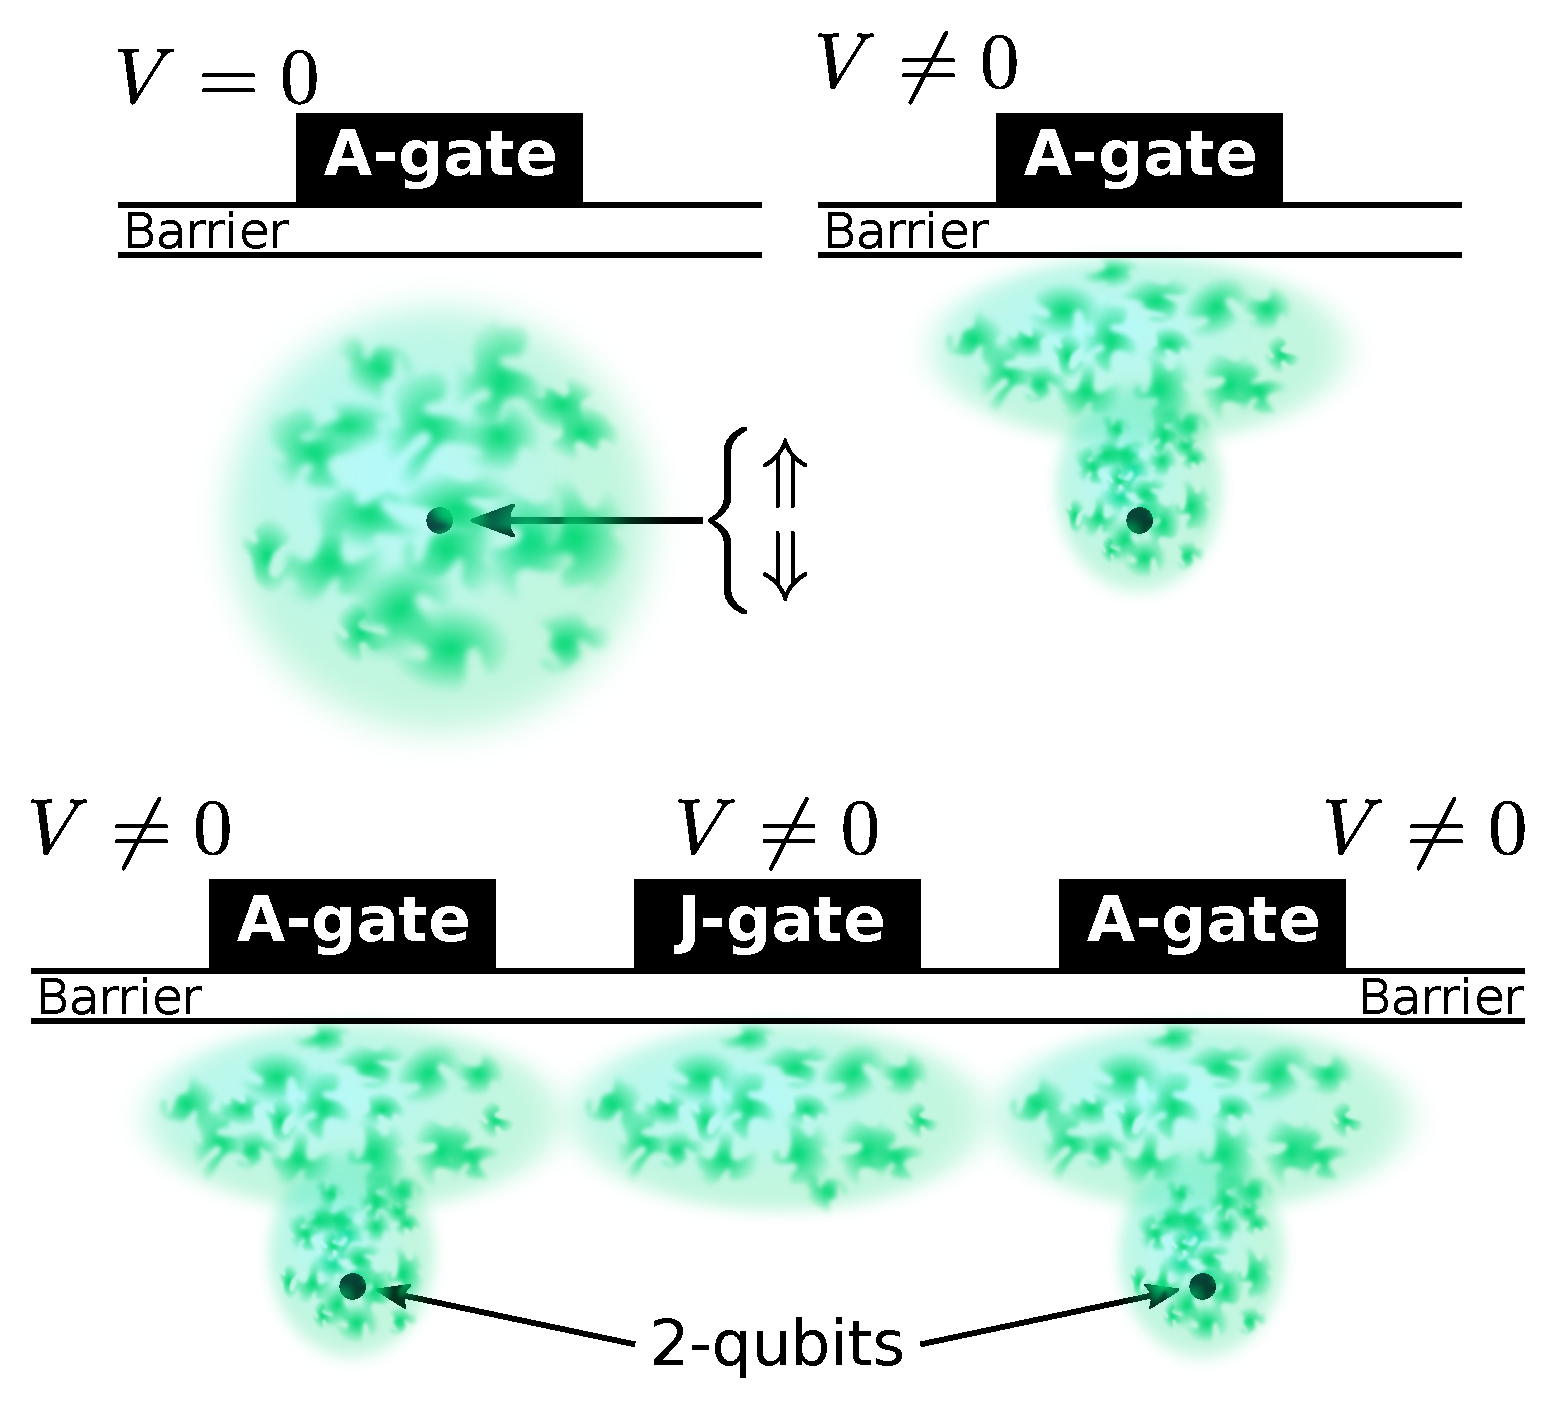
\includegraphics[width=0.45\textwidth]{introduction/figures/kane.pdf}
\vspace{-7pt}
\caption{Sketch of the Kane's proposal for a silicon-based nuclear spin quantum computer. An electric gating $A$ controls the hyperfine interaction by increasing/decreasing the electronic density around the nucleus, allowing the isolation of the nuclear spin on demand. Similarly, an inter-qubit gate allows the interconnection of different qubits.}
\label{kane_proposal}
\end{wrapfigure}
\FloatBarrier
%~~~~~~~~~~~~~~~~~~~~~~~~~~~~~~~~~~~~~~~~~~~~~~~~~~~~~~~~~~~%
Kane's proposal: ``Silicon-based nuclear spin quantum computer'' deals with the first requirement in the following way. The quantum information is to be stored in the nuclear spin of Phosphorus atoms inserted in a matrix of Silicon ($\ce{Si}:\leftidx{^{31}}{\ce{P}}$). The $\ce{Si}$ was selected for its abundance of isotopes with nuclear spin $I=0$ in addition to the huge industry behind it, ensuring the know-how to manipulate this material as needed. Once the host material was chosen, the options for donors were quite limited, in fact it turns out that the only shallow donor in $\ce{Si}$ with nuclear spin $I=1/2$ is Phosphorus and, in particular, the isotope $\leftidx{^{31}}{\ce{P}}$. In addition, a number of studies\cite{Feher1959, Wilson1961, Waugh1988} show that its nuclear spin relaxation time can exceed 10 hours, and it is likely to be as high as $10^{18}$ seconds for lower temperatures. % phonon

When $\ce{P}$ dopants are introduced in $\ce{Si}$, an electron is confined in the vicinity of the dopant. The extension of such state can be as large as hundreds of ångströms so, if there are several dopants in the same area, the electronic states can act as an effective coupling among their nuclear spins\cite{Slichter1990}.

% Three external parameters are necessary for this proposal: \begin{enumerate*}\item an electric gate above each donor to control the strength of the hyperfine interaction and, hence, the resonance frequency of the nuclear spins beneath them \item electric gates between the donors to turn on and off electron-mediated coupling between the nuclear spins \item a globally applied A.C. magnetic field to flip nuclear spins at resonance.\end{enumerate*}

In order to control the interactions in this system an electric gate on top of each of the dopants is required. The electronic states could be deformed in the vicinity of the $\ce{P}$ nucleus, as shown in \fref{kane_proposal}, increasing/decreasing the hyperfine interaction resulting in a shift of the resonance frequency for the spin flip.
The interaction between different qubits could be switched on and off using electric gating as well although its implementation requires, among other things, the dopants to be at a very specific distance (with atomic precision), which is definitely a challenge in this platform. Similarly the idea is to increase/decrease the electronic density in the inter-qubit space in order to allow/prevent the propagation of the spin information.
% XXX finish
% Morello? Experimental status?


This approach takes advantage of the naturally weak interactions with the nuclear spin and the high tunability of the surrounding electronic states.
The coupling of the nuclear and the electronic spin is mediated by the hyperfine interaction so the spin state can be transferred between the nucleus and the electrons.

Another big challenge is the detection of the spin time at any given time of any of the components. Although there is not an ultimate answer for this problem, there are many ideas to work around it. The simplest option could be the use of a number of qubits all in parallel so the macroscopic magnetization could be measured. If the nuclear spins are incorporated into an electronic devices it is possible to infer the nuclear spin based on the electronic properties.\cite{Kane1992,Wald1994,Stich1996,Dixon1997,Dobers1988,Stegner2006}.

\section{Our proposal}
Our proposal replaces the $\ce{P}$ dopants in $\ce{Si}$ by $\ce{H}$ adatoms on bilayer graphene.
This system provides the same ingredients: a host with virtually no nuclear spin impurities,\footnote{The abundance of Carbon isotopes with nuclear spin $I=0$ is $\sim98.9\%$ while this number for Silicon is $\sim92.2\%$}, a dopant with nuclear spin $I=1/2$ and a surrounding electronic spin $S=1/2$ spatially bounded to them.

The purer composition of $\ce{C}$ will translate in less decoherence for the $\ce{H}$ nuclear spin, resulting in longer relaxation times. The nuclear-electron interaction is mediated by the hyperfine coupling which only exists for $s$-orbitals, and the $1s$ level is the one binding the electron closest to the nucleus, making $\ce{H}$ a good candidate.
%
At the same time, the chemisorption of the $\ce{H}$ adatom binds strongly its electron to the $\pi$ electrons of graphene, removing most of it from the $s$-orbital, luckily the occupation of this orbital is highly tunable via electric gating. This tunability is a key element for this proposal since it is the mechanism that will allow us to switch on and off the interactions with the qubits.

The electronic states in graphene (and graphene bilayer) are known to be highly tunable, in particular an external electric field would allow the control of the relevant properties in this system such as the localization length of the electronic states.

% XXX picture of the system

The initial reason to consider this system was the possibility of opening a band gap upon the application of an external electric field\cite{McCann2006, Castro2007, Oostinga2007, Zhang2009, Taychatanapat2010, Castro2010a, Ponomarenko2011, Allen2012, Sui2015}.
This conductor to insulator transition provides a handy knob to control the localization length of the electronic states which results in the control of its effective electron-electron interactions as well as the interactions with the nuclear spins.

Another advantage of using $\ce{H}$ adatoms on top of bilayer graphene over $\ce{Si}:\leftidx{^{31}}{\ce{P}}$ is that nowadays there are methods to place the $\ce{H}$ adatoms with atomic precision and in a reversible way\cite{elias2009,Brihuega2016,Brihuega2017}. In particular around 20 $\ce{H}$ atoms have already been placed in a single sample and, in principle, there should be no physical limit since the process could be automatized for larger arrays.
\medskip

The study of the tunable interactions in this system led us to the realization that $\ce{H}$ adatoms on bilayer graphene provide a framework where localized states can be placed at will and where the interactions among them are highly tunable upon the application of an external electric field.
Such a system is the ideal playground to implement physical realizations of a wide variety of hamiltonians, the ultimate goal for analog quantum simulations.
%The ability to engineer physical system to realize model hamiltonians is a long wished goal in the analogue quantum simulations community.
In particular, our analysis show that by carefully choosing the placement of the adatoms (the distance and relative position among them) one can engineer the electron-electron interactions to explore both weakly and strongly interacting systems.
\bigskip

This situation in which we can create localized electronic states at will and engineer the electron-electron interactions is specially appealing after the recent discovery of an unconventional superconducting phase in twisted bilayer graphene\cite{Cao2018,Cao2018a}.
Even though it will not be discussed in the thesis, it is worth pointing out the similarities between our proposal and the newly found twisted bilayer graphene physics.
In order to get superconductivity in twisted bilayer graphene two requirements are to be met. First, the twisting angle needs to take a very low (and particular) value. This requirement ensures the emergence of a Moire pattern which is responsible for the localization of electronic states in the boundaries between domains. This localized states result in the emergence of (almost) flat bands all over the Brillouin zone and very close to the Fermi energy. Second, the fine tuning of the filling factor is key to place the Fermi level in the middle of the flat bands and conveniently tune the electron-electron interaction.

The resulting phase diagram is quite similar to that of the cuprates family what may suggest a similar microscopic mechanism for superconductivity to appear. The big difference is that while cuprates are a somewhat complex material, the chemistry of graphene has been very well known for a long time, and the behavior of the $p$ orbitals (rather than $d$ orbitals) is much simpler.
The low energy effective model of graphene is probably the most studied in the history of Condensed Matter Physics so one may expect that studying the complex problem of unconventional superconductivity would be easier in this case.

Nevertheless, it looks like superconductivity will not give up its secrets so easily since, even though the low energy Hamiltonian of graphene is very well known, its extension to the twisted bilayer is not so easy.
It is probably too soon to tell but the introduction of superconductivity in the graphene/2d-materials community my be a game changer for this hundred year old problem of superconductivity.


\section{Scope of this thesis}
This thesis approaches these systems mainly from a computational point of view.
%
%Condensed Matter Physics is an immensely broad topic. It encompasses many different systems at different scales and with many different approaches.
%This thesis sits on the theoretical side and is essentially computational, nonetheless it might have the flavor of Applied Physics or even Material Science. Naturally many other paths could have been followed, experiments pursued, theoretical models deepened and many topics could be further studied, but the line has to be drawn at some point.
%
Through out the whole thesis the driving force has been sometimes the possibility of interesting results, regardless their ``immediate'' utility, and some times the possibility of real world application in the near/mid future.
This position, midway between fundamental research and real world applications, might be a bit uncomfortable since experimentalists or industry-oriented people might find it a bit vague or hypothetical whereas fundamental researchers might think of it as too narrow, or even missing the big picture.

In contrast I think this ``equidistance'' provides a privileged position to explore a number of interesting topics without loosing touch with experimental reality.
\bigskip

This thesis revolves around graphene and graphene-based systems, with a special focus on the applications of a particular case: bilayer graphene.
%One can find a number of reasons for choosing graphene: it is (was) a relatively new material, it has many physically interesting properties and the potential for plenty of applications, it draws a lot of attention form the research community...
One could say that the scientific community may have gone through an ``interest bubble'' involving graphene and, as a consequence, it has been advertised as a miraculous material with the potential to change the world as we know it. I will not address the controversy of the almighty properties of graphene but I would like to briefly address the graphene hype within the scientific community.
In order to have a somewhat quantitative description of the graphene hype I have analyzed the book of abstracts of the APS March Meeting since 2005 until 2019.\footnote{notice that 2018 is missing since I could not find the pdf for the full book of abstracts}
The analysis counts the number of abstracts containing a given term (or groups of terms) and normalizes the count to the total number of abstracts that year.
This quantity is a very rough estimate, of course, but the resulting count is arguably related to the interest of the condensed matter community on a certain topic.

%~~~~~~~~~~~~~~~~~~~~~~~~~~ FIGURE ~~~~~~~~~~~~~~~~~~~~~~~~~%
\begin{figure}[!ht]
\centering
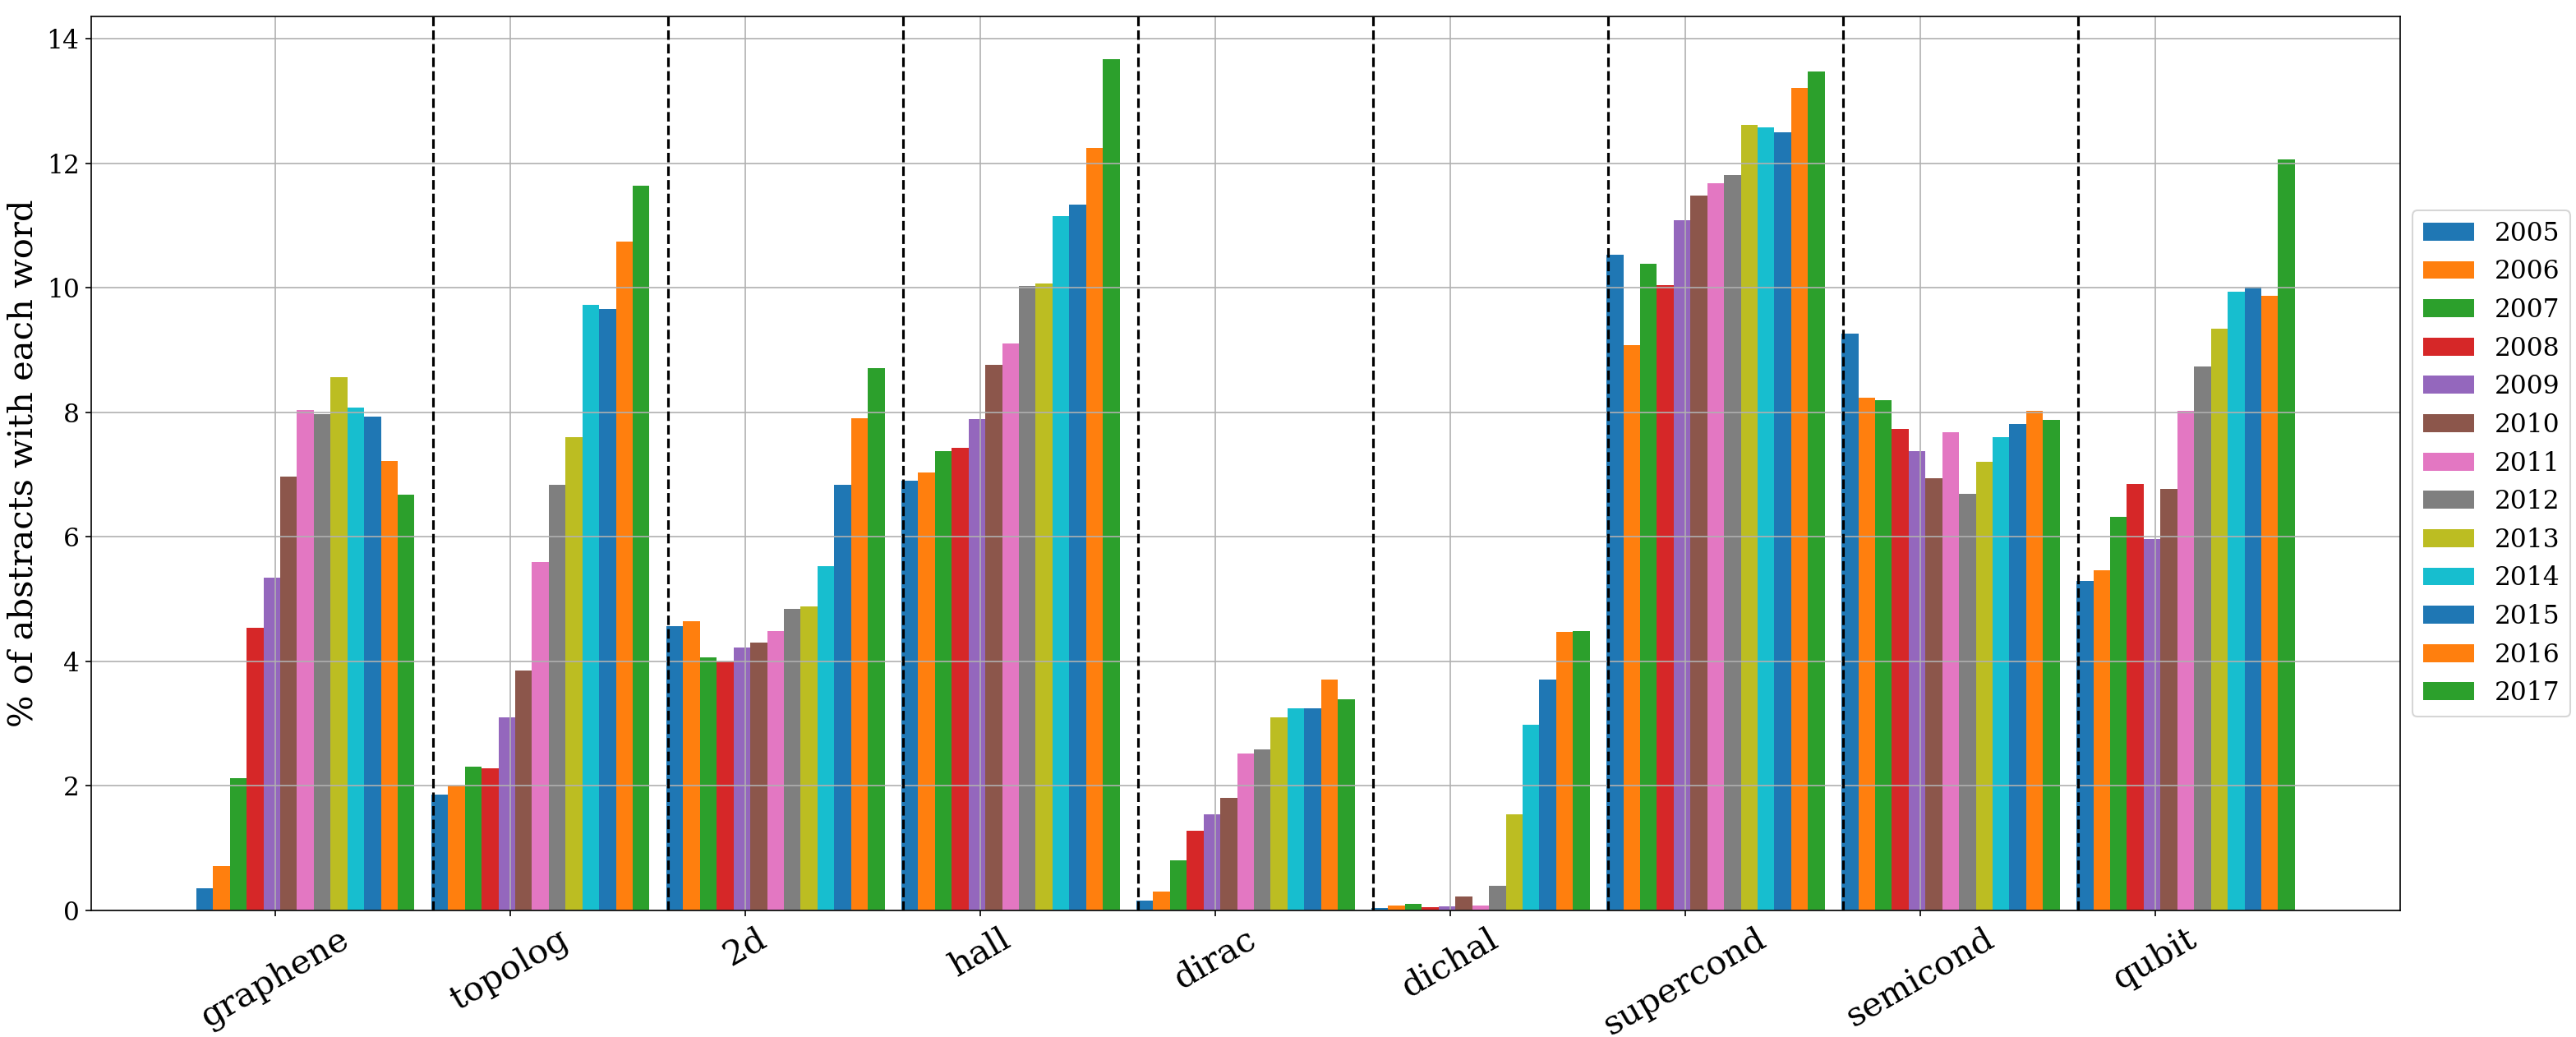
\includegraphics{introduction/figures/topics.png}
\vspace{-20pt}
\caption{Evolution through out the years of different topics at the APS March Meeting. The plot was done by counting the number of abstracts containing a given word and normalizing it by the total number of abstracts in the conference. Note that the bars are placed in chronological order for each item.}
\label{topics}
\end{figure}
%\FloatBarrier
%~~~~~~~~~~~~~~~~~~~~~~~~~~~~~~~~~~~~~~~~~~~~~~~~~~~~~~~~~~~%

The case of graphene, first block of bars in \fref{topics}, is very interesting, since one can see its raise since (almost) its discovery and the beginning of its decay. This trend is a strong indicator of a possible interest bubble, but I would like to point out the trend over the years of the terms next to it in \fref{topics}: topolog\textcolor{gray}{[y,ical]}, 2d, dirac, \textcolor{gray}{quantum-,spin-,anomalous-}hall, dichal\textcolor{gray}{cogenides, $\ce{MoS2}$, $\ce{WS2}$, $\ce{WSe2}$}\footnote{the terms in grey are grouped during the counting process}.
All of these terms are undoubtedly related to graphene an clearly they show a steadily growing trend.
\medskip

Graphene itself is very interesting and it probably deserves all the fame and attention that it gets, but I would argue that the importance of graphene lies in the fact that it has become the gateway for many other materials and even research branches.

The understanding of graphene has been the spark to start the race of two dimensional materials research. \ac{2dm} are a very interesting family of materials both form an applied point of view and from the perspective of fundamental research.
On one hand, any industry-related property (conductance tunability, magnetism...) becomes instantly interesting just because its 2D nature ensures smaller sizes and possibly cheaper products.
On the other hand their 2D nature place them right in the frontier between the classical and quantum regime: they are macroscopic (sometimes reaching millimeters) but being one atom thick there are non negligible quantum effects all over the place, what makes the fascinating from the fundamental physics point of view.
Since the discovery of graphene many other bidimensional materials have been synthesized: $\ce{MoS2}$, $\ce{WSe2}$, $\ce{MoT2}$, $\ce{BN}$, $\ce{CrI3}$, $\ce{NbSe2}$, $\ce{TaS2}$, $\ce{MnBi2Te4}$... each with their unique set of properties and its list of possible applications in the rapidly growing field of Quantum Technologies. % Footnote to the flagship?
%But everything started with graphene.
Some of these materials will be mentioned during the thesis, but graphene will be the common thread through out the thesis.
%\bigskip


%One of the most interesting properties of graphene is that, being two dimensional, it is all surface, and electrons living in surfaces respond strongly to external perturbations.
%If a superconductor is placed nearby, electrons in graphene will behave in a superconductor way\cite{},
%if placed on top of an insulator it will develop a gap\cite{}, if subjected to an external field its electronic states will be heavily modified.
%A material in which so many different states may appear is interesting in itself, so it is no wonder why having such a panoply of different phases at their disposal, scientists quickly thought of the possibility of mixing different 2D materials in order to engineer properties at will\cite{Geim2013}.

%In the spirit of these combined structures, commonly known as Van der Waals heterostructures, this thesis extensively explores the properties and applications of a bilayer of graphene.
%TODO meh....change
%\bigskip



% The reason to focus on bilayer graphene was that it presents a property that is really hard to find in other materials. Bilayer graphene undergoes a transition from conductor to insulator in the presence of an electric field.
% Opening and closing a gap is a very powerful resource when dealing with electronic states since it affects the spatial localization of the electrons and many properties depend on this. In particular it is very interesting to consider a number of quasi-localized electronic states placed at the correct distance for the change in localization via gap-opening to influence their interactions.
% Even, going one step further, it is not far-fetched to think of an scenario in which we can combine the this tunable gap with some spin interactions being able to tune the electronic states for each spin channel independently.
% \bigskip


%Considering this playground of tunable gaps and electrically controlled  localization lengths we considered the role of defects in bilayer graphene and their behavior under the influence of external fields. In particular Hydrogen, $\ce{H}$, chemisorbed adatoms will play a major role in this thesis.
%
%This kind of defects produce quasi-localized electronic states around them, and the localization length of these states is strongly determined by the band gap in the system. Without going into much detail for now, we focused in the spin interactions in such a system. On one hand the chemisorbed $\ce{H}$ atoms trap a single electron ($S=1/2$) in their vicinity, on the other hand, their nucleus consists of a single proton ($I=1/2$), and the interaction between them is controlled, again, by the spreading of the electronic state.

\bigskip
A complete list of my publications:
\begin{itemize}
   \item Coupling of the $\ce{As}$ $A_{1g}$ phonon to magnetism in iron pnictides\cite{Garcia-Martinez2013}

   \item Interaction-driven phases in the half-filled spinless honeycomb lattice from exact diagonalization\cite{Garcia-Martinez2013a}

   \item Quantum spin Hall phase in multilayer graphene\cite{Garcia-Martinez2015}
   \item Edge states in graphene-like systems\cite{Lado2015}

   \item Anomalous magnetism in hydrogenated graphene\cite{Garcia-Martinez2017}

   \item Real-space mapping of topological invariants using artificial neural networks\cite{Carvalho2018}

   \item Electrical spin manipulation in graphene nanostructures\cite{Ortiz2018}

   \item Van der Waals spin valves\cite{Cardoso2018}

   \item Exchange rules for diradical $\pi$-Conjugated Hydrocarbons\cite{Ortiz2019}

   \item Designer fermion models in functionalized graphene bilayers\cite{Garcia-Martinez2019}
\end{itemize}



\bigskip
The rest of this thesis is structured as follows. \chref{ch:graphene} and \chref{ch:bilayer} review the basic properties of graphene and bilayer graphene respectively, as well as most of the methods of calculation used along the thesis.

\chref{ch:vacancy} is based on the publication [\cite{Garcia-Martinez2017}] and it explores a number of properties of $sp^3$ defects on graphene.

\chref{ch:vacancy_bilayer} expands onto the effects of $sp^3$ defects on bilayer graphene.

\chref{ch:hyperfine} explores the tunability of the hyperfine coupling

\chref{ch:designer} studies the possibilities of $\ce{H}$ adatoms on bilayer graphene as a platform to perform analogue quantum simulations.






%Following these lines, this thesis has somewhat been driven by a proposal dating all the way back to 1988\cite{Kane1988} on how to build a \emph{quantum computer}. In this proposal Bruce E. Kane suggested Phosphorus impurities in Silicon ($\ce{Si}:\leftidx{^{31}}{\ce{P}}$) as the building block for a silicon based nuclear spin quantum computer.

%Any proposal for building quantum computers (or qubits, for that matter) has to deal with the conflict between two opposing requirements. On one hand we need the qubits to be well isolated from the environment so interactions with the outside world does not affect the quantum state of the computer. On the other hand, we need to be able to interact strongly and quickly with the qubits in order to change or read its state.

%The idea to tackle this contradiction was to use the nuclear spin (1/2) of the $\leftidx{^{31}}{\ce{P}}$ to store information, due to the relatively low concentration of nuclear spins in the system, and the electric cloud around them as mediators among $\ce{P}$ impurities.
%The way to control the interactions would be based on the application of electric gates which would distort the electronic states increasing or decreasing the hyperfine interaction (coupling between the nuclear and the electronic spin) as well as tuning the electronic configuration in between defects.
%\medbreak

%Ignoring the specific nature of the materials involved, the relevant ingredients in this proposal are a nuclear spin 1/2, which is expected to be isolated from the rest of the universe upon the application of an electric field, An electronic spin 1/2 located somewhat around the nuclear spin and with a big response to an electric field so the interaction between the two spins can be highly tuned.
%\bigskip







%%%%%%%%%%%%%%%%%%%%%%%%%%%%%%%%%%%%%%%%%%%%%%%%%%%%%%%%%%%
%\newpage
%We are today on the verge of a technological revolution, a quantum leap\footnote{pun intended} that holds the promise for a revolution in chemistry, pharmacology, telecommunications, virtually any application in which optimization is a problem and even Condensed Matter Physics itself.
%But let us start from the beginning.
%\medbreak

%The laws of \ac{qm} started developing at the beginning of the XX century. At that moment, it was commonly thought that only a few details in the laws of Physics remained unexplained, but as Physicists delved deeper in these unexplained phenomena (namely the photo-electric effect and the black body radiation), it became clear that there was some missing piece.

%Step by step it was found that as the energy scales of the experiments grew smaller, the well-founded laws of \emph{classical} physics started failing.
%% infrared catastrophe
%% atomic model (electron radiation)
%The development and understanding of the laws of \ac{qm} was fast and in merely 30 years there were entire research fields centered already in different aspects or applications of it.

%Of particular interest to this thesis is the line of material science and condensed matter physics research. Prior to the understanding of \ac{qm}, there was no theory to explain the properties of any material.
%Whether a piece of rock was able to conduct heat or electricity was essentially a matter of trial and error. Of course some experimental observations led Chemists to build a collection of somewhat empirical laws and group elements based on similar properties, but there was no microscopic understanding of the mechanisms leading to these properties.

%The capabilities of \ac{qm} to predict electronic properties of different materials led to a revolution in science, technology and ultimately society. The extensive research on semiconductor materials during the 1960s was key to the invention of the transistor: a device that can block or allow the flow of electrical current at will.

%The transistor is the basic building block for any electronic device. Nowadays there are millions if not billions of transistors in our computers or smartphones, but only a few thousand were enough to send 3 humans to the moon (and back!). For the last 50 years, transistors have operated based on the fine-tune of the band population of two neighboring materials creating an effective potential barrier between them preventing electrons to move freely.
%As the electronic industry developed the need for smaller transistors became apparent, the smaller the transistors are, the more can be fit in a particular device.
%This race towards miniaturization pushed the development of new materials and techniques to size down transistors all the way to the current\footnote{In mass production, there are plenty of claims for smaller transistors.} $\sim\SI{14}{\nm}$. As expected, when we shrink the components of the transistors, we approach a limit in which quantum effects irrelevant until now may take a major role. The simplest obstacle that the shrinking of transistors have to deal with is the quantum tunnel effect, by which the electrons would be able to flow through the potential barrier, rendering the transistor unable to effectively stop electric current.

%Quantum effects will play an important role as technology shrinks, but this may not be necessarily a problem.
%\medbreak

%Quantum limit is a feature. Feynman "control of atomic properties"

%Quantum computers

%Quantum simulations


%%%%%%%%%%%%%%%%%%%%%%%%%%%%%%%%%%%%%%%%%%%%%%%%%%%%%%%%%%%%%%%%%%%%%%%%%%%%%%%%%
%\newpage
%The development of Quantum Technologies has barely started and it already promises a revolution in many different fields, from medicine and pharmacology, computation, encryption, any application in which optimization is a problem and even the understanding of quantum mechanics itself.
%There is probably nothing riskier than trying to make technological predictions, but even governments around the world are taking action to be in the forefront of this revolution\cite{QTF} and big companies such as Google, IBM or Microsoft are investing huge amounts of money in these topics. But let us start from the beginning.
%\medbreak

%% Quantum technologies
%Nowadays we are barely getting a glimpse of the potential of quantum technologies to impact technology and science in general, but Quantum computation is not something that we just thought about.
%Ever since we started the race to shrink every computer component, we headed towards the limit of quantum computation. A transistor is a device able to switch on and off an electrical current on command. They are the basic building block for any kind of computerized device. The first transistors were macroscopic, some centimeters and wired by hand. As the potential of computers grew, the need to create more, cheaper and smaller transistors launched the race for miniaturization. %Moore's Law is the empir
%Nowadays a single transistor is the size of a few nanometers. At this scale  quantum effects start playing a significant role.
%If there is a potential barrier stopping the electric current and it becomes smaller and smaller at some point the tunnel effect will be probable enough to render the transistor unable to stop any electric current at all.
%This is one of the simplest limitations that computers face as we miniaturize components.
%
%While it may seem that dealing with the inevitable quantum effects is a big inconvenience, scientists began to consider the possibility of using these effects to our benefit.
%The first ideas about the possibilities for quantum computing started in the 80s and 90s\cite{Benioff1980, Feynman1982, Manin1980, Shor1994} showed that a quantum computer could tackle problems that a classical computer simply could not.
%
%Since then there has been huge developments both theoretical and experimental towards the realization of a platform in which to perform \emph{quantum computations}.
%\medbreak

%% Graphene
%In general, states near surfaces are very susceptible to external biases. In particular, \ac{2d} materials present highly manipulable electronic states since they only have the surface to live in.
%Even before its discovery, graphene has drawn a lot of attention. Many of its properties were expected well twenty years before its experimental discovery. While it is arguably true that there has been an over-hype bubble around its supposed miraculous applications, it is definitely true that graphene has been the gateway towards a whole new realm of phenomena in condensed matter physics.
%
%Initially most of its interest relied in the expectancy of a new Hall phase emerging without the need of an external magnetic field\cite{Kane2005a,Ostrovsky2008} and the experimental observation of the \ac{qhe}, a macroscopic effect of a purely quantum phenomenon\cite{Zhang2005}.
%Also fact that some high-energy physics models were naturally realized in graphene was a huge motivation for this material to hoard the attention of a big part of the condensed matter community.

%Certainly graphene has many interesting properties, but when two layers of graphene are placed one on top of each other there is a property that will be central for the development of this thesis.

%Graphene bilayer is the only known material which can open a gap upon application of an electric field. It has been shown that an electric


%\newpage
%In order to start wrapping our minds around this Quantum Revolution, we need to look back to the beginning of the XIX century. Back then Physics was consider to be completely understood, except for a couple of seemingly simple experiments, namely the photoelectric effect and the black body radiation. These phenomena were the gateway to discover the realm of Quantum Mechanics.

%Many experiments followed and the theory was not left behind. Soon we had a framework with the mathematical tools to describe all these new phenomena. Nevertheless having the basic laws that rule this

%\medbreak
%The world has seen all sorts of revolutions all throughout history. While not necessarily every revolution has turned the world into a better place, when we account just for the scientific or technological revolutions, this is usually the case.

%%At the end of the XVIII century, the invention of the steam engine and its later introduction in the industrial processes allowed a huge step forward for many societies and, for better or worse\cite{}%climate
%%, reshaped the world.
%%The Industrial Revolution changed the way we travel and work, it changed the scale at which humans interacted with the planet and, arguably, the universe.
%%The whole world has seen how virtually any index measuring quality of life has been raising ever since\cite{}.\footnote{Sadly this trend has not been homogeneous at all around the globe and these changes have been much more clear in some countries than others.}

%%Similarly, another huge revolution came along with
%The worldwide introduction of computers in most households and the construction of a worldwide web interconnecting ``everyone'' in the world has been one of the biggest revolutions over the last 30 years. The information technologies have changed the job-market landscape, the way humans learn, shop, the way we socialize even the way we fight wars. Even in their first stages computers were able to put two men on the moon and bring them back with less computational power than the cheapest smartphone available today.
%Our daily habits, our leisure time, even crucial historical events\cite{Alhindi2012} have been determined by the use of computers and the internet.
%
%For this revolution to happen, many agents had to be in place. The need for secure communication channels during World War II pushed the development of information theory and the later Cold War pushed scientists and engineers to build computers. But the bare necessity is not enough to develop the necessary technology. The first computers used \emph{macroscopic transistors} and \emph{macroscopic bits} when they were introduced. At first these essential pieces were handmade and manufactured one by one. It was not until the research in semiconductor physics developed microscopic versions of these pieces that the computers became cheap and easy to produce.
%\medbreak
%
%\newpage
%For nowadays computers to exist, it was necessary the development of Quantum Mechanics. Starting with the beginning of the XX century, physicist realised that Physics was not completely understood but rather there were many mysteries when
%
%
%
%Naturally these revolutions did not just happen, it took many years of hard work and research to stablish the basis for these technologies to emerge. In particular, for computers to be created and be popularized it was necessary a deep understanding of the laws of quantum physics which led to the mastery of the semiconductor technologies.
%
%
%
%\newpage
%
%%%%%%%%%%%%%%%%%%%%%%%%%%%%%%%%%%%%%%%%%%%%%%%%%%%%%%%%%%%%%%%%%%%%%%%%%%%%%%%%%
%The relation between research in fundamental Physics and technological innovations is not always easy to see. In the best of cases, it usually takes some years, at least a few decades, for fundamental research to find its way into the industry.
%While this is a completely fair question, it is quite short-sighted. Let us think of the latest revolution that changed our society.
%The introduction of computers in our everyday life and the access to a global network of communications was a revolution, maybe even comparable to the industrial revolution.
%
%We have had computers in most households for the last 30 years, broad access to the internet for over 20, yet, trying to pin-point the fundamental research that took us there is quite hard, if not impossible.
%We can think of the first transistor\footnote{actually there is a previous patent, from 1930,\cite{diode} but no hard proof that it was ever built or used.},
%the building block of every electronic device, which would take us to the 40's\cite{Ross}, but it would be unimaginable to reach that point without at least some understanding of the physics of semiconductors which had been studied for the previous 50 years. It would be insane trying to understand semiconductors without, at least, a few notions of quantum mechanics, electromagnetism...
%We could line up all the most brilliant minds of humanity that set the path towards today's technology: Landau, Bardeen, Bloch Dirac, Heisenberg, Bragg, Brillouin, Faraday, Gauss... countless others... Ask them about the application of their research, and not one of them would be able to describe a personal computer or the internet.
%
%That is why asking the researchers about the usefulness of their research is like asking newborn babies what will be their job position in 42 years time.
%
%Of course we have our own vision of what the research may bring upon the world, but let us keep in mind that this vision is nothing but a childish dream, since time and time again the applications have exceeded the wildest expectations of the researchers.\\
%
%
%At the end of the XIX century it was believed that Physics was solved. Today we know it is not. In particular, Condensed Matter Physics is an area in which even when we know the physical laws governing every interaction there is still much that we do not understand. Quantum Mechanics gives us the tools to describe any problem that we want to describe. From superconductors to topological phases or spin liquids, the Hamiltonian is known and yet we cannot solve it. The last fifty or sixty years of condensed matter physicist have been devoted to approximations and simplifications that would allow us to strip the problems to its basic components in an attempt to understand the microscopical mechanism behind so many interesting phenomena.
%The thorough investigation of a variety of problems while not completely successful in every area, has had a great side effect. The cumulative experience of decades of condensed matter physics research has granted us the ability to control matter with atomic precision in a wide range of situations. The fulfillment of such a dream\cite{Feynman1982}
%
%Quantum technologies\cite{QTF}
%
%The research on semiconductor physics can be hard to pin-point,
%
%
%In this work we study a variety of properties regarding defected graphene bilayer. Starting from the basic concepts of graphene, we build our way to the role of sp$^3$-defects in graphene bilayer such as chemisorbed Hydrogen adatoms.
%First we study the properties of these defects one by one in isolated scenarios. Then we wonder the effects of neighboring defects


%~~~~~~~~ Chapter ~~~~~~~~
%~~~~~~~~ Chapter ~~~~~~~~
\chapter{Graphene}
\label{ch:graphene}

%
% TODO
% - Comparison bands 4 orbital 1 orbital
% - Dirac description?
%
%2) Background chapter (90%)
%   - TB 1 orbital
%  - TB 4 orbitales
%   - SOC (origin in 4 orbital model)   Connection between the 2D graphene with SOC and 4 orbitals,  the  gap= sublattice* spin*valley,  the Kane & Mele model  for G. Monolayer.
%   -  Graphene monolayer + Bilayer
%   - Topological phases (Z2, edge states, Kane Mele model)

This chapter aims to provide a self-contained introduction to the methods we use to model graphene as well as some of its most interesting/relevant properties. Specifically, I present the tight binding models that are used throughout the thesis. A more extended description of these methods and properties can be found in several reviews since graphene is one of the most studied materials in history\cite{KatsnelsonBook, Geim2007, Murakami2009, CastroNeto2009a, Mas-Balleste2011, Konschuh2011a, Cooper2012, Han2014, Sadurni2014, Rozhkov2016,Novoselov2004, Novoselov2005}.
Even before its experimental discovery, extensive research was devoted to it\cite{Wallace1947, VanBommel1975, Semenoff1984, Haldane1988, Forbeaux1998, Oshima2000}.
All the basic properties have been discussed profusely, yet, for the sake of completeness, I will make a brief recap of all the properties relevant for the rest of this thesis.
\medskip

%XXX
% Graphene properties summary
% 0 gap semiconductor
% ambipolar field effect
% dirac electrons
% Hall
% large mobility
% mechanical properties

% 2 modelos, 1 orb, 4 orb, SK
Graphene consists of a two-dimensional array of carbon atoms arranged in a honeycomb structure\cite{Huang2011} % TODO more references
like the one shown in \fref{graphene_summary}(a,b).

%~~~~~~~~~~~~~~~~~~~~~~~~~~ FIGURE ~~~~~~~~~~~~~~~~~~~~~~~~~%
\begin{wrapfigure}{R}{0.5\textwidth}
\centering
\vspace{-10pt}
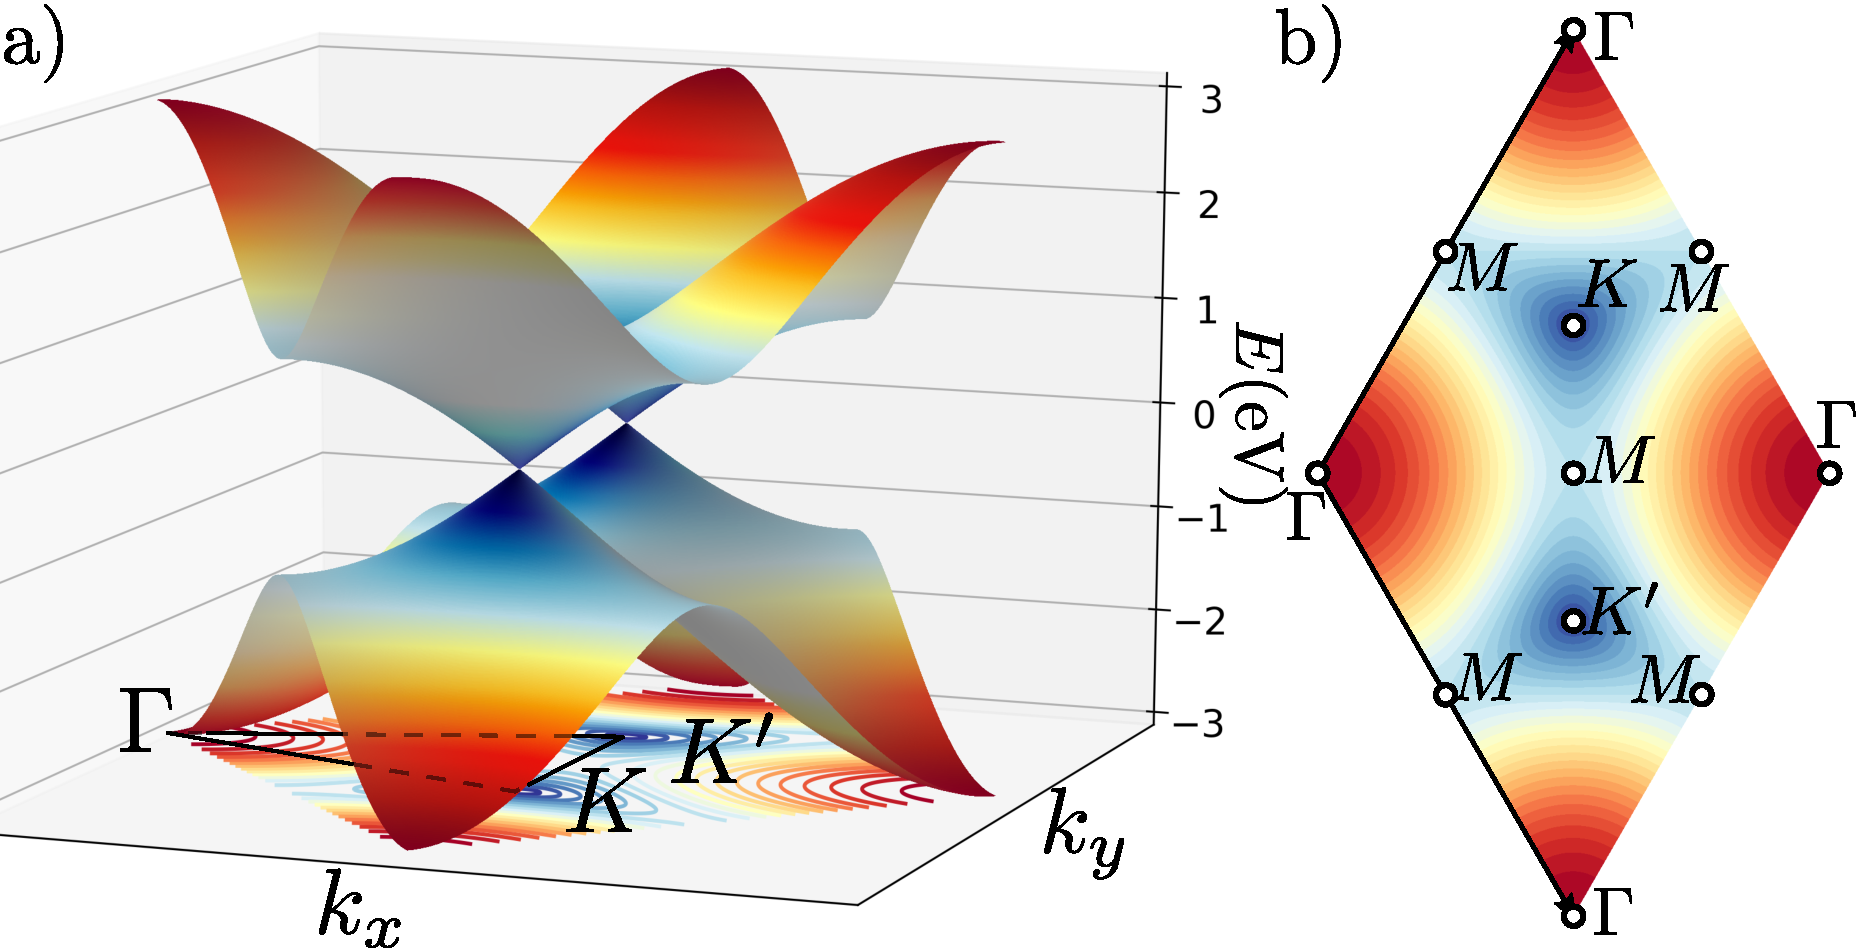
\includegraphics[width=0.48\textwidth]{graphene/figures/bands_min.pdf}
\vspace{-7pt}
\caption{a) Band structure of graphene over the whole Brillouin Zone. Notice the cones in the $K$ and $K'$ points. b) Contour plot over the Brillouin Zone marking the high symmetry points.}
\label{G_bands_min}
\end{wrapfigure}
\FloatBarrier
%~~~~~~~~~~~~~~~~~~~~~~~~~~~~~~~~~~~~~~~~~~~~~~~~~~~~~~~~~~~%

It has a peculiar band structure featuring two pairs of opposing cones touching exactly at the Fermi level. There are two main characteristics to highlight from this configuration, first, that the pairs of cones meet in a single point at the Fermi energy, and second, that the dispersion of the band structure is exactly linear for low energies.

This band structure is very unusual since its is different from both conductors and instulators. On the one hand it has available states for conduction infinitesimally close to the Fermi level (like a metal) but, on the other hand, it has no Fermi surface (like a semiconductor or an insulator). For this reason it is usually defined as a zero-gap semiconductor.

The linear dispersion of the band structure is responsible for the strong modulation of the electric conductivity upon the application of an electric field. This phenomenon, usually known as field effect, is due to the strong doping induced via electric gating, which moves the Fermi level across the cones resulting in an important increase of the carriers density available for conduction which can be either electrons or holes since the band structure is symmetric around the Fermi Energy (electron-hole symmetry).
\medskip

The linear dispersion is of special interest not only for the condensed matter community but also for the high energy. The electrons  subjected to this linear dispersion are mathematically equivalent to having massless spin $1/2$ particles obeying the Dirac's equation. This equivalency is quite straightforward from the analytical calculation of the tight-binding and is explored in detail later on.
\medskip


Another consequence of the band structure is that the observed \ac{qhe}\cite{Zheng2002,Zhang2005,Gusynin2005,Peres2006a,Brey2006,Fertig2007,Ostrovsky2008,Fujita2016} is different from the one in conventional semiconductors on 3  counts: first, it shows symmetric \ac{ll} for electrons and holes; second , it has a "zero" \ac{ll}, third, the quantization pattern has an extra 1/2 that arises from the non-trivial Berry phase of Dirac electrons
% Graphene presents a half integer \ac{qhe} due to the topological nature of its band structure, which arises from a non-trivial Berry phase.

Graphene is expected to be a \ac{ti}\cite{Blick2019}, meaning that when all the interactions are taken into account, particularly the \ac{soc}, a very small band gap is predicted to open at the Dirac point, in the order of a few $\si{\micro\eV}$ although not measured experimentally, possibly due to temperature smearing and device precision.\cite{Kane2005,Min2006}
This gap nonetheless is not a standard insulating band gap. In finite samples the band structure would appear gaped everywhere, but two conducting channels would appear on the edges of the sample.
This conducting states, spatially bounded to the edge of the system, are the so-called topological edge states and are known to be robust against any perturbation (that does not close the gap by breaking time-reversal symmetry).  %XXX check

% XXX to chapter 1
Appendices \ref{ch:QSH} and \ref{ch:ANN} are two of my published papers which expand on these topics. The first explores the topological character of few-layer-graphene exploring the proximity effect of different materials. The second explores the bulk-edge correspondence\cite{Hasan2010} using neural networks to estimate the topological phase of some systems based only on a subset of the density matrix corresponding to the bulk region.



\section{Basic definitions}
Unless otherwise stated, we will consider that the unstrained atomic distance between carbon atoms is $d_{\ce{C}-\ce{C}}=a=\SI{1.4}{\angstrom}$ in accordance with literature\cite{KatsnelsonBook, Cooper2012, Ishigami2007}. % TODO more biblio

%~~~~~~~~~~~~~~~~~~~~~~~~~~ FIGURE ~~~~~~~~~~~~~~~~~~~~~~~~~%
\begin{figure}[!ht]
\centering
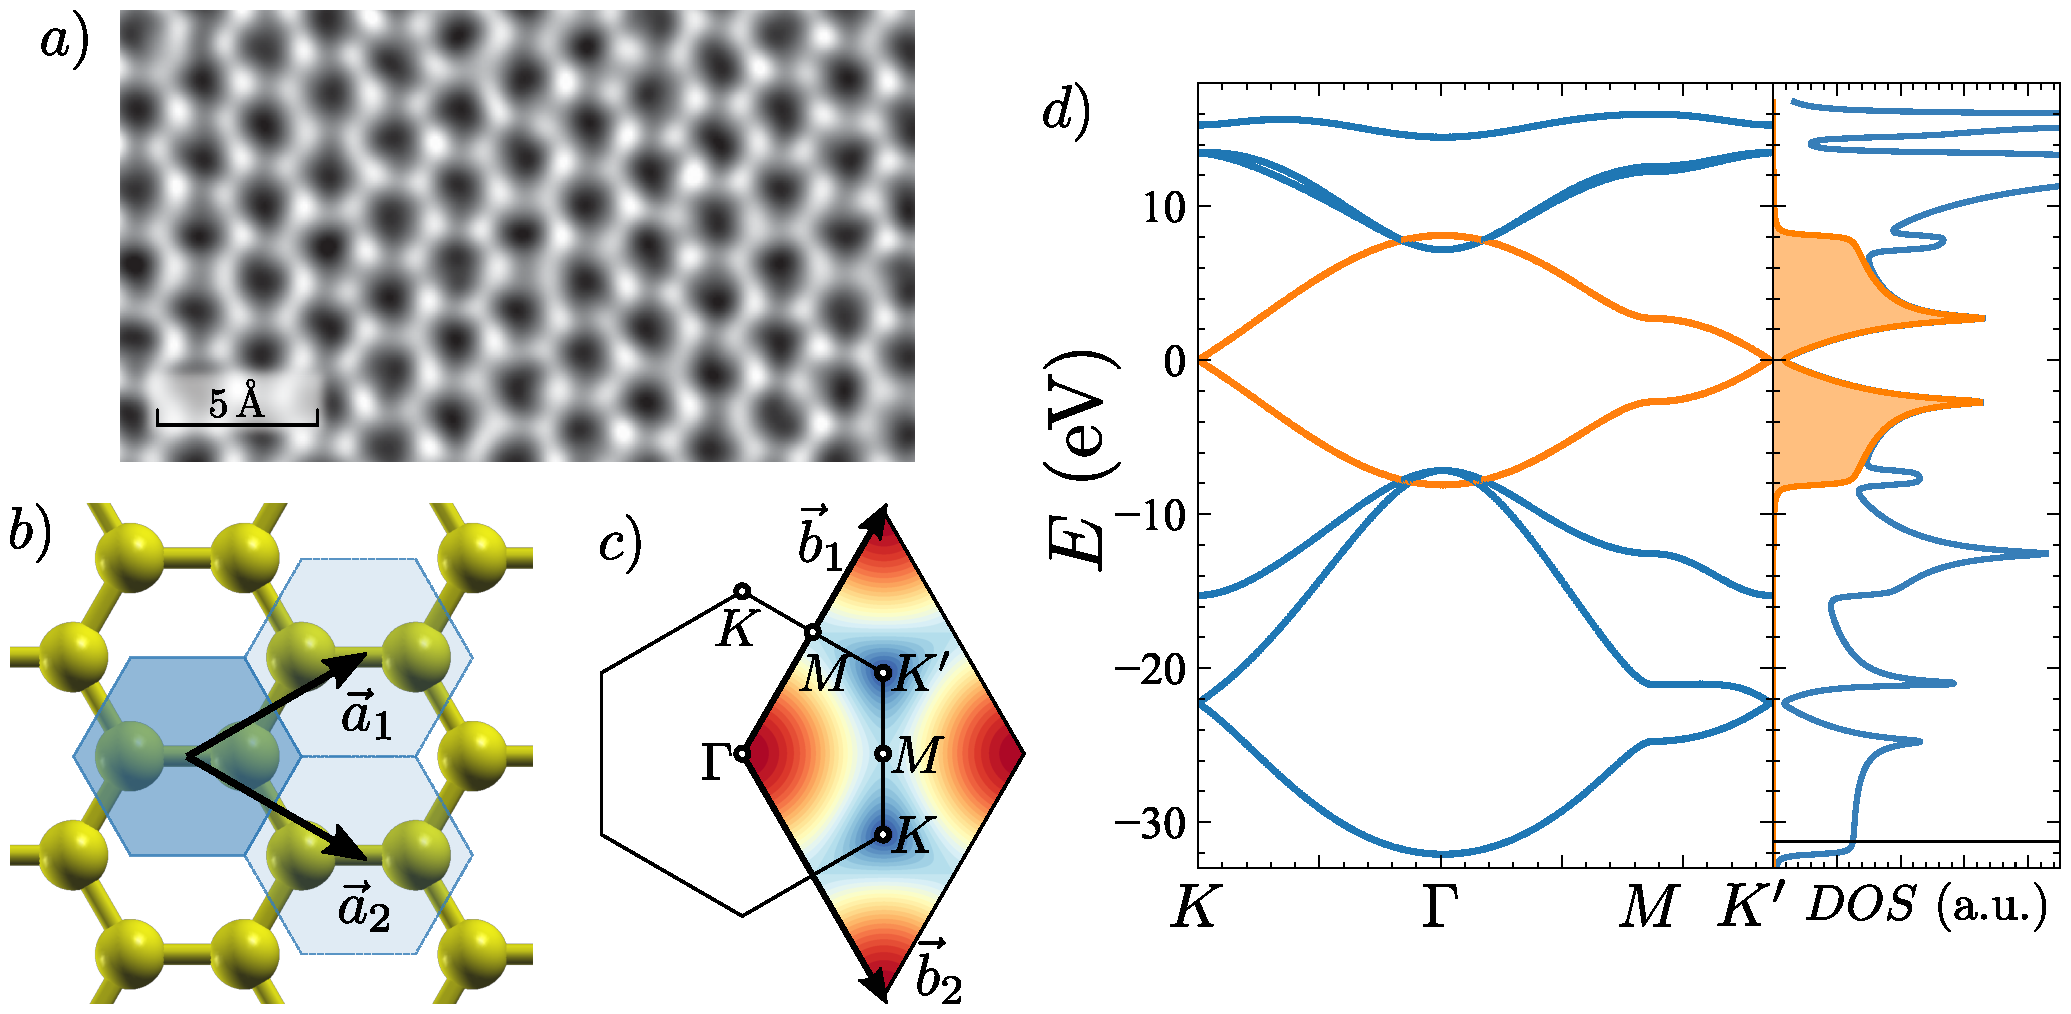
\includegraphics{graphene/figures/graphene_summary.pdf}
\vspace{-5pt}
\caption{$a)$ STM image of graphene taken from ref~\cite{Huang2011}. $b)$ Cartoon depiction of the atomic structure of graphene using the lattice vectors defined in \eqref{latt_vec} and the Wigner-Seitz cell. $c)$ Reciprocal vectors $\vec{b}_i$ and two representations of the FBZ. $d)$ Band structure and DOS of graphene calculated in the tight-binding approximation (details later in the text).}
\label{graphene_summary}
\end{figure}
% \FloatBarrier
%~~~~~~~~~~~~~~~~~~~~~~~~~~~~~~~~~~~~~~~~~~~~~~~~~~~~~~~~~~~%

The honeycomb structure is not a Bravais lattice so, in order to describe the system in terms of Bloch functions, we have to choose a unit cell and the appropriate lattice vectors to tessellate the space.
Naturally there are infinite possibilities to do so, but the simplest one is that depicted in \fref{graphene_summary}b).
%The simplest unit cell and  Bravais lattice with which we can describe graphene is the one depicted in \fref{graphene_summary}a).
It consists of two atoms per unit cell and a triangular lattice. We will consider the following atomic positions:
\begin{equation}
\vec{r}_a = \tfrac{a}{2}(-1,0,0) \quad;\quad
\vec{r}_b = \tfrac{a}{2}(1,0,0),
\label{at_pos}
\end{equation}
The lattice vectors that define the triangular Bravais lattice are, then:
\begin{equation}
\vec{a}_1 = \tfrac{a}{2}\left(3,\sqrt{3},0\right) \quad;\quad
\vec{a}_2 = \tfrac{a}{2}\left(3,-\sqrt{3},0\right)
\label{latt_vec}
\end{equation}
This geometry defines a hexagonal Wigner-Seitz cell (blue region on \fref{graphene_summary}b)) with area $\sim\SI{5.1}{\angstrom\squared}$. The reciprocal lattice vectors are depicted in \fref{graphene_summary}c) and can be easily calculated using the relation\cite{Ashcroft1976}: $\vec{a}_i\vec{b}_j=2\pi\delta_{ij}$. Notice that the canonical \ac{fbz} shown in \fref{graphene_summary}c) is an hexagon (just like the Wigner–Seitz cell) but nothing changes if we use the colored rhomboidal region instead, which is much more convenient for computational calculations.
\medbreak


Once the atomic and lattice structure is clear, we turn to the electronic properties. Carbon atoms have 6 electrons allocated in five orbitals distributed in the layers with quantum number $n\in\{1,2\}$.
The first two electrons are in the $1s$ level, two more in the $2s$ level and finally another two \acp{el} in the three $2p$ levels (\fref{orbitals}).
%~~~~~~~~~~~~~~~~~~~~~~~~~~ FIGURE ~~~~~~~~~~~~~~~~~~~~~~~~~%
\begin{figure}[!ht]
\centering
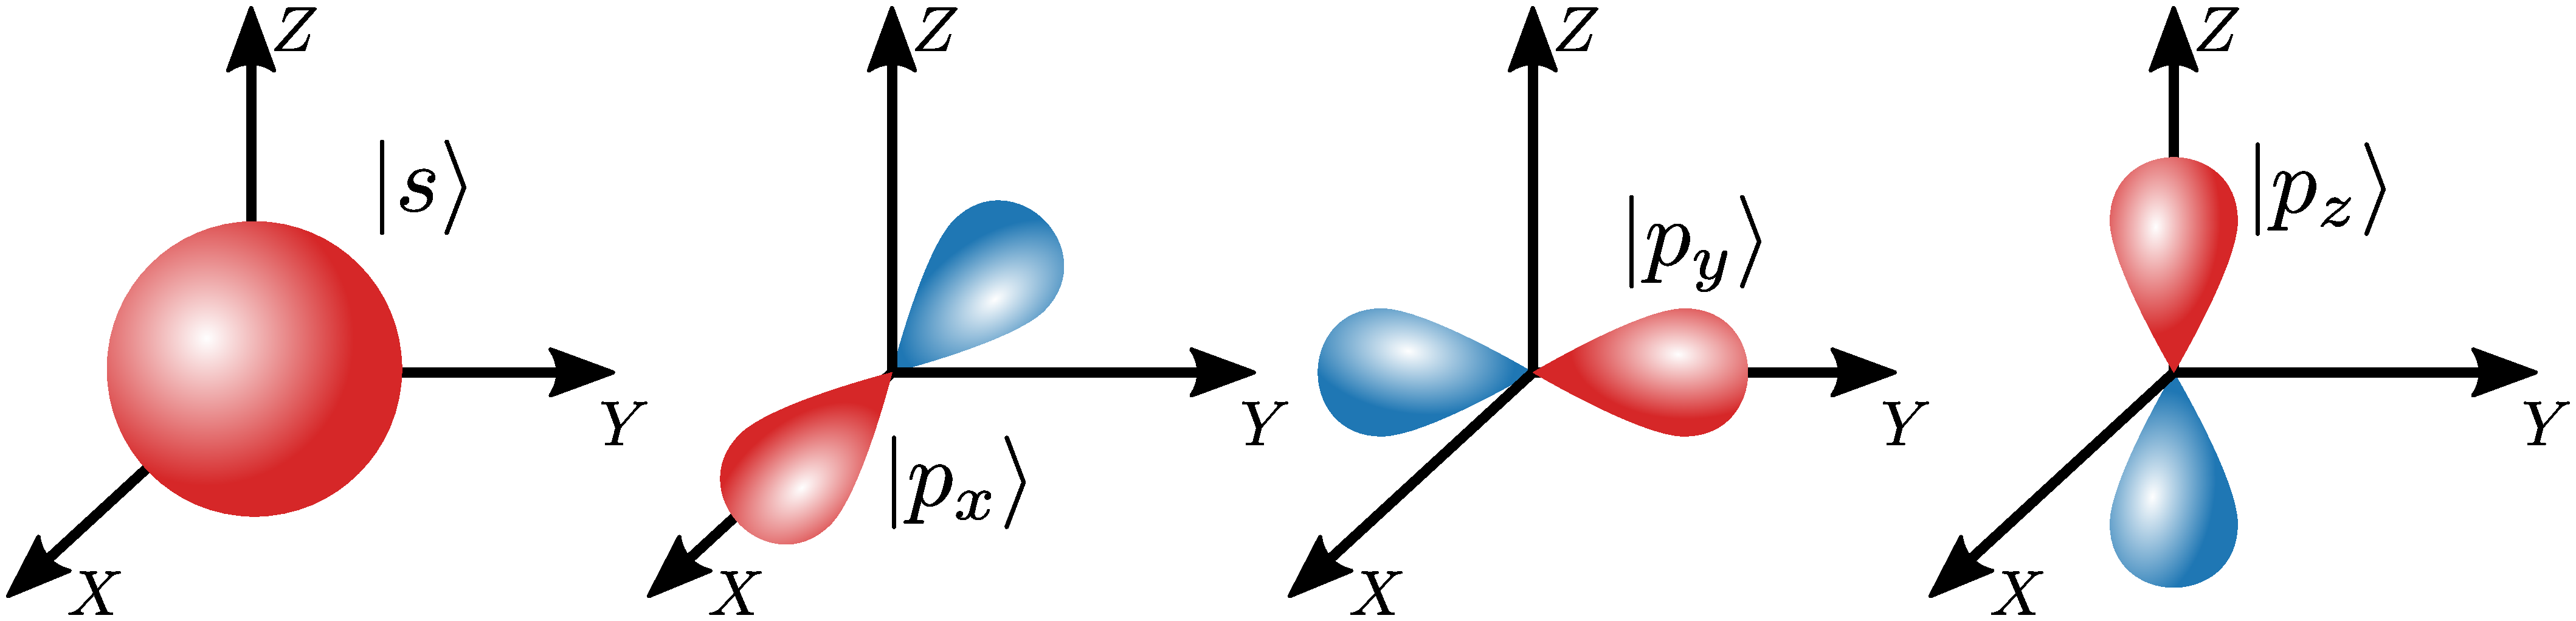
\includegraphics{graphene/figures/orbitals.pdf}
\vspace{-5pt}
\caption{Cartoon depiction of the hydrogenoid orbitals involved in the graphene chemical and physical properties. The color of the orbitals shows the parity of the orbital what will be relevant when building tight-binding models.}
\label{orbitals}
\end{figure}
% \FloatBarrier
%~~~~~~~~~~~~~~~~~~~~~~~~~~~~~~~~~~~~~~~~~~~~~~~~~~~~~~~~~~~%
Since the orbitals $n=1$ are doubly occupied and far down in energy, there is no need to consider them. The $2s$ level is also full, but they show a strong hopping with neighbouring $p$ orbitals which are around the Fermi energy so we will consider their contribution. The $2p$ orbitals are the closest to the Fermi level, hence they will play a major role in the chemistry of graphene.
\medbreak

With this description of the system we can build a basis which will have four orbitals per Carbon atom:
\begin{equation}
  \mathcal{B}_4 = \left\{
  \ket{\phi^1_{s}},\ket{\phi^1_{p_x}},\ket{\phi^1_{p_y}},\ket{\phi^1_{p_z}},
  \dots,
  \ket{\phi^n_{s}},\ket{\phi^n_{p_x}},\ket{\phi^n_{p_y}},\ket{\phi^n_{p_z}}
  \right\}
\label{basis4}
\end{equation}
where the superscript points out the atom and the subscript shows the corresponding orbital. The bands calculated in the \ac{tb} approximation resulting from this description are shown in \fref{graphene_summary}d). We will delve in the physical properties later on, but for now it should suffice to point out the linear dispersion in the $K$ and $K'$ points around the Fermi energy (taken always as $E_F=\SI{0}{\eV}$) as well as the decoupling of the two bands involved in the low energy regime. These two bands (colored in orange) are composed exclusively by $p_z$ orbitals as it can be seen in the \ac{dos} (side panel of \fref{graphene_summary}d)).
\smallskip

In many cases it is enough to describe the two bands closest to the Fermi energy since the phenomenon at hand is restricted to the low energy region. In those cases we will reduce our basis and consider only the $p_z$ orbitals, resulting in the basis:
\begin{equation}
  \mathcal{B}_1 = \left\{\ket{\phi^1_{p_z}}, \ket{\phi^2_{p_z}},\dots, \ket{\phi^n_{p_z}}\right\}
\label{basis1}
\end{equation}
\medskip

There are a number of ways to build a \acf{tb} Hamiltonian. When using the single orbital basis \eqref{basis1} the hopping parameters are a single scalar and it is enough to fit the band width to estimate it, but for a more complex description using the four orbital basis \eqref{basis4} the estimation of the parameters is not so easy. In the next section we show the details for the Hamiltonian models used all along this thesis.


\section{Slater-Koster tight-binding model}
\label{ssec:SK}
In general, the hopping parameters are an input in any \acf{tb} model. They are usually calculated by fitting eigenvalues (and possibly eigenfunctions) obtained from \ac{dft} calculations. Another way to calculate the hopping parameters is to project the \ac{dft} eigenfunctions into a basis of localized atomic orbitals so the interpretation in terms of hydrogenoid orbitals is easier.

As a system grows complex, more and more parameters are needed to describe it. In fact, the number of hoppings grows with the size of the basis, $n_\mathcal{B}$, as $\sum^{n_\mathcal{B}}_i i$. Nevertheless since the number of different orbitals is finite and a larger basis means only a more complex arrangement of orbitals, one could expect that not every parameter is completely independent from the others.
%~~~~~~~~~~~~~~~~~~~~~~~~~~ FIGURE ~~~~~~~~~~~~~~~~~~~~~~~~~%
\begin{figure}[!ht]
\centering
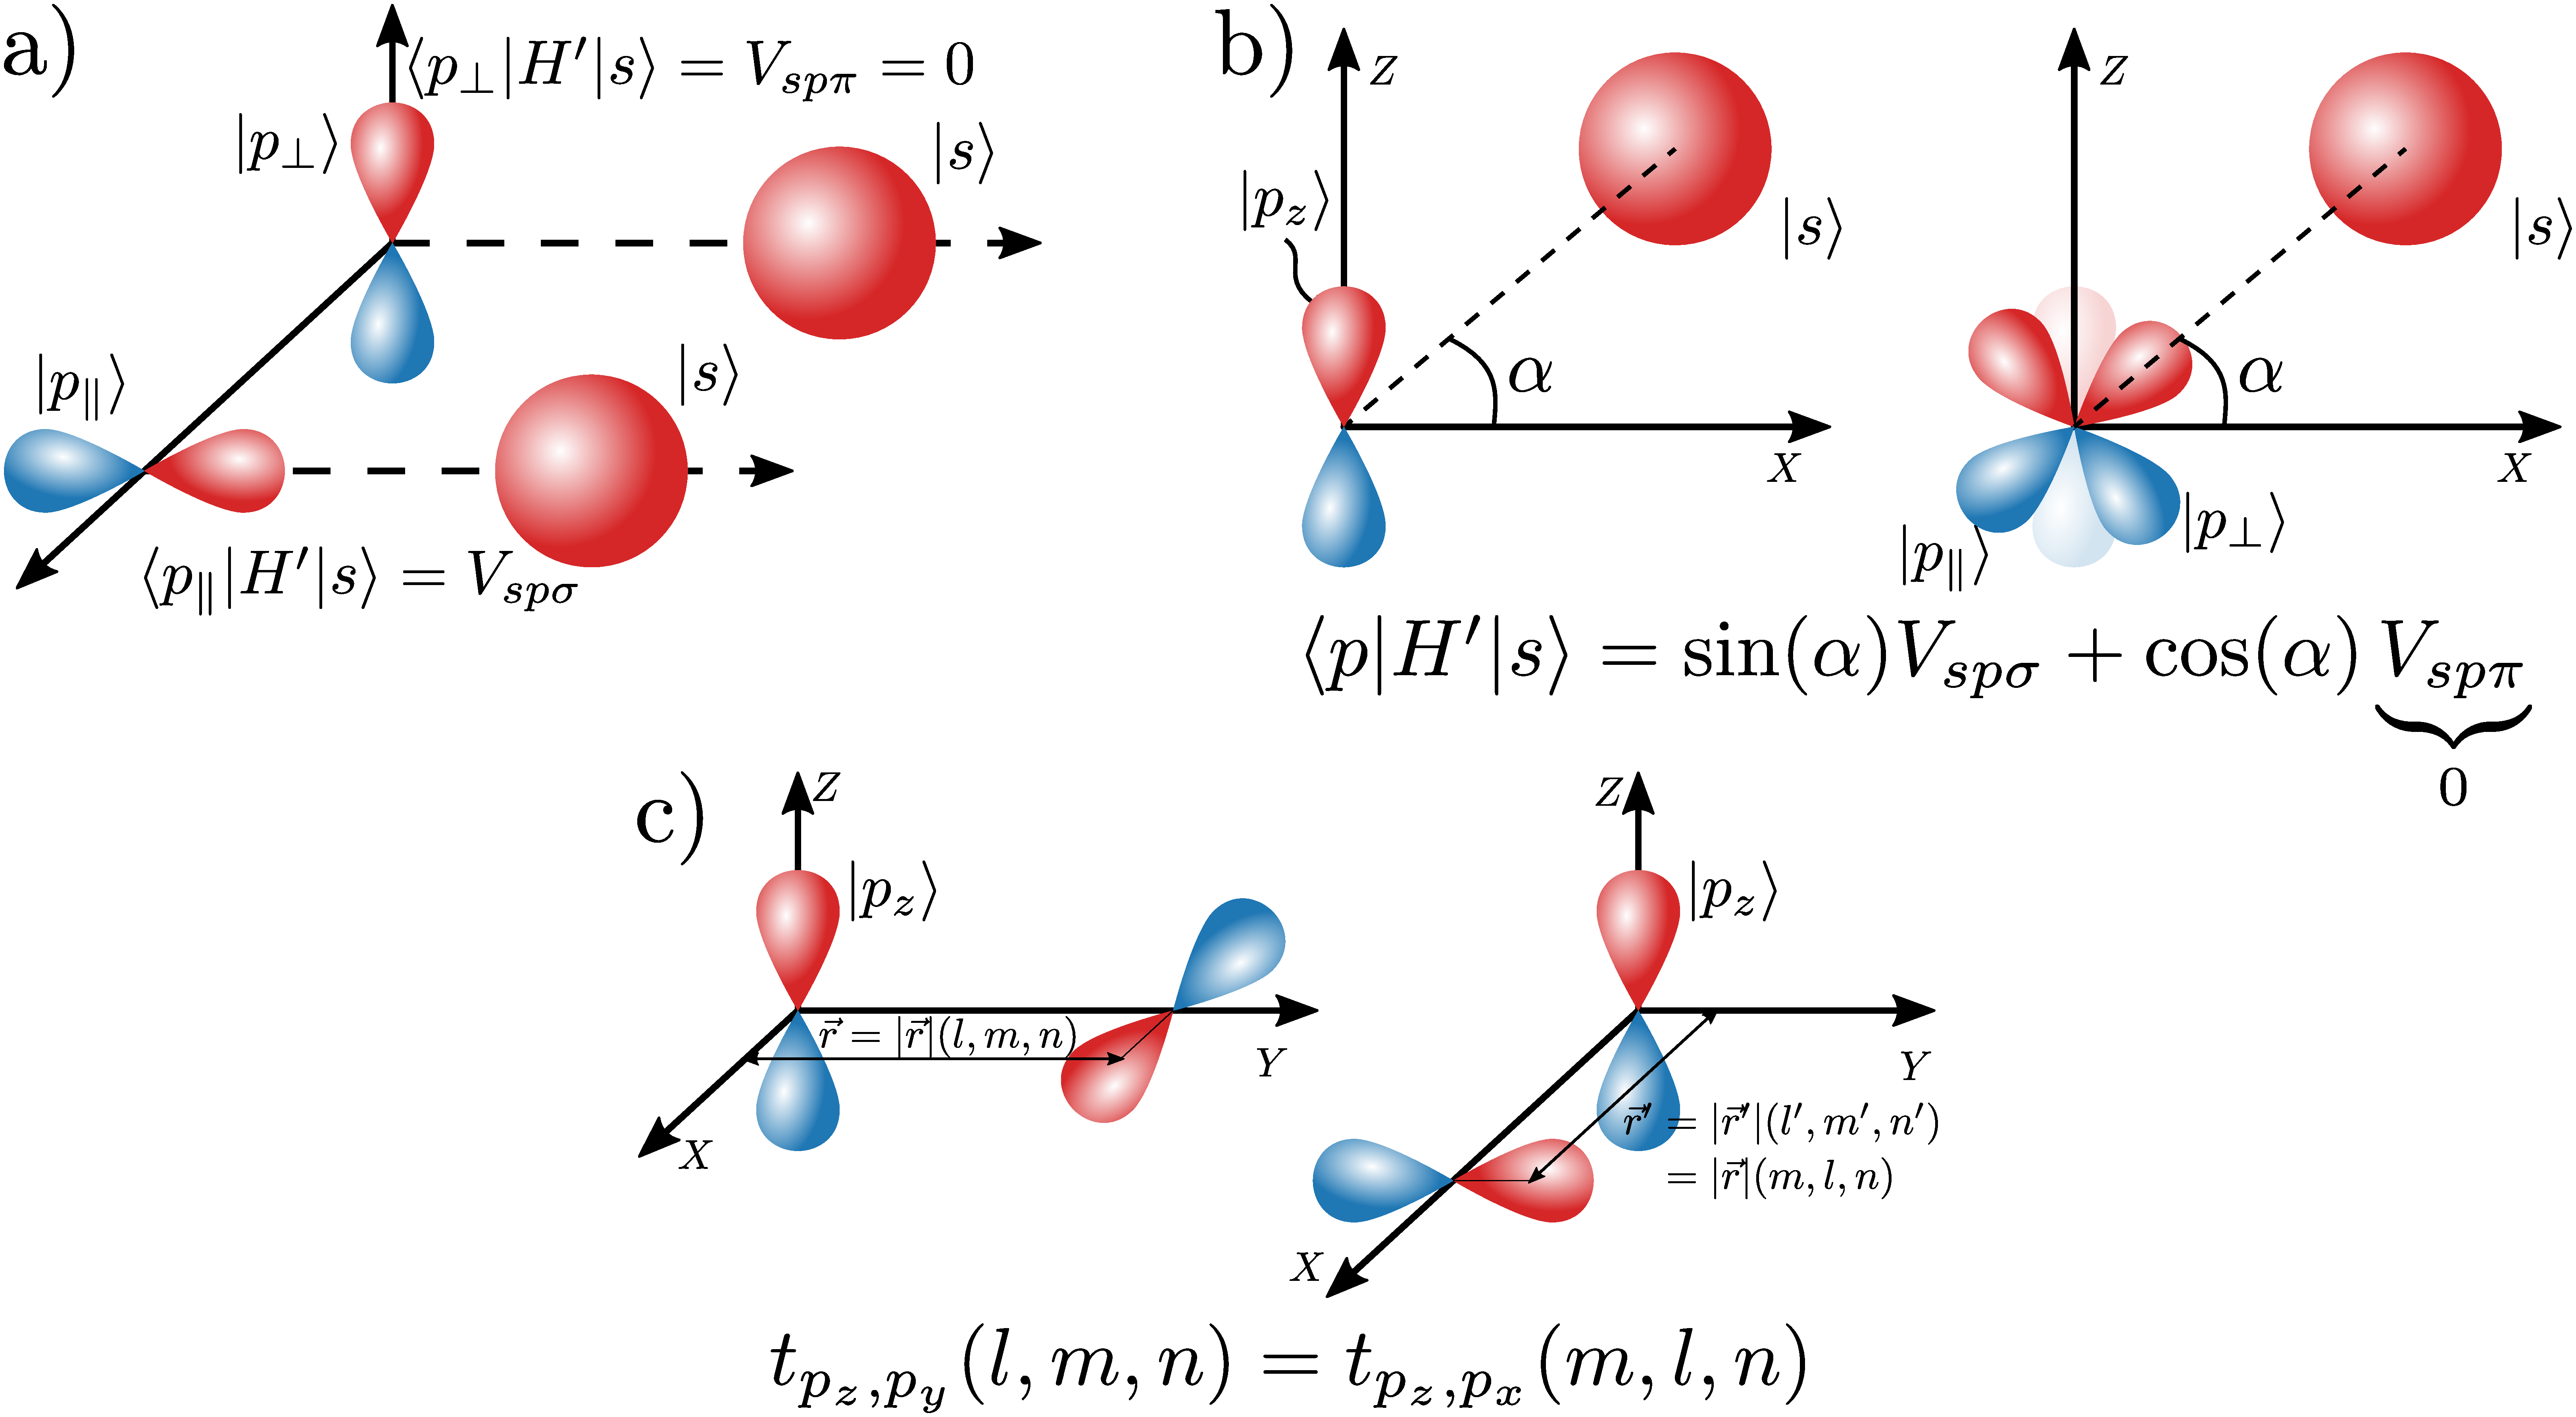
\includegraphics[width=0.85\textwidth]{graphene/figures/hoppings.pdf}
\vspace{-5pt}
\caption{$a)$ Definition of the parallel and perpendicular hoppings. Notice that $V_{sp\pi}=0$ because of the symmetry of the orbitals (integral of the product of an even and an odd function). $b)$ Decomposition of a $p_z$-$s$ hopping in terms of its parallel and perpendicular projections. $c)$ These two hoppings must have the same value regardless of the definition of the axes. This is the way \ac{sk} hoppings are derived from one another.}
\label{fig:SK}
\end{figure}
% \FloatBarrier
%~~~~~~~~~~~~~~~~~~~~~~~~~~~~~~~~~~~~~~~~~~~~~~~~~~~~~~~~~~~%
The \ac{sk} approximation\cite{Slater1954} takes into account the symmetry of the atomic orbitals to reduce the number of parameters needed since some of them are related by rotations or other symmetry operations.

In the \ac{tb} approximation the two-center hopping integrals\cite{Ashcroft1976, Grosso2000},
$$t_{\phi_1-\phi_2} = \bra{\phi_1(\vec{r})}H'(\vec{r},\vec{r}')\ket{\phi_2(\vec{r'})}$$
express the probability of an electron to transition between two orbitals, due to the inter-atomic interactions contained in $H'$. In the \ac{sk} approcimation these integrals are encoded in a set of constants:
% where $H'$ encodes all the (interacting) terms outside of the atomic Hamiltonian, are encoded in the \ac{sk} approximation as a set of constants:
% The \ac{sk} model encodes the two-center hopping integrals\cite{Ashcroft1976, Grosso2000} 
% $$t_{\phi_1-\phi_2} = \bra{\phi_1(\vec{r})}H'(\vec{r},\vec{r}')\ket{\phi_2(\vec{r'})}$$
% along high symmetry directions in a set of constants:
$V_{\alpha\alpha'm}$, where $\alpha$ and $\alpha'$ label the orbitals and m refer to the component of angular momentum along the line between the center of the two orbitals. Two examples of these constants, $V_{sp\pi}$ and $V_{sp\sigma}$\footnote{Notice that in graphene $V_{sp\pi}$ automatically vanishes because of the symmetry of the orbitals.}, are shown in \fref{fig:SK}a).

It is important to notice that the radial information, \ie the distance between atoms, is enclosed in the \ac{sk} parameters $V_{\alpha\alpha'm}$, while the angular dependence, \ie the atomic positions, provide the functional dependencies in the \ac{sk} model. For instance, if we focus on the hopping between two $p_x$ orbitals\cite{Slater1954} separated by a distance $\vec{r}=|\vec{r}|(l,m,n)$:
\begin{equation}
  t_{p_x-p_x}(\vec{r})=  t_{p_x-p_x}(l,m,n) = l^2 V_{pp\sigma}(r) + (1-l^2) V_{pp\pi}(r)
\end{equation}
The radial information (distance between atoms) will be encoded in the numerical values of $V_{pp\sigma}$ and $V_{pp\pi}$ while the geometrical information of the lattice will be contained in the factors $l^2$ and $(1-l^2)$

Since we are neglecting lattice vibrations the distance dependence of the parameters can be safely ignored but, as a rule of thumb, one can consider that the \ac{sk} parameters will decrease as the distance between the orbitals increases.
The exact ratio depends on the orbitals and the crystalline structure, and different approximations can be found in the literature\cite{Harrison1930}, but $V_{\alpha,\alpha'm}(r)\sim1/r^5$ is a standard estimation.
\bigbreak


The \ac{sk} description of the \ac{tb} hopping integrals allows the formulation of every hopping in terms of a few parameters which encode the distance between orbitals while preserving the angular information in the analytical formulation which has been reproduced from the original publication in appendix \ref{SKhoppings}.
\medbreak


% XXX ~~~~~~~~~~~~~~~~~~~~~~~~~~~~~~~~~~~~~~~~~~~~~~~~~~~~~~~~~~~~
By projecting the hopping integrals into its parallel and perpendicular components (see \fref{fig:SK}b)) we reduce the number of parameters needed to account for all possible hoppings. For instance, we only need two parameters: $V_{pp\sigma}$ and $V_{pp\pi}$ in order to express all six $p-p$ hoppings.

This description of the hopping parameters also accounts for the symmetry of the orbitals. For instance \fref{fig:SK}c) shows the relation between the hoppings $t_{p_{z},p_{x}}$ and $t_{p_{z},p_{y}}$. If we forget about the labels in the axis, we can realize that these two hoppings are in fact equivalent since one can be obtained as a rotation of the other.

If we define the unitary vector $\hat{r} = \vec{r}/|\vec{r}|$ and its components $\hat{r}=(l,m,n)$ we can see that
\begin{equation}
  t_{p_{z},p_{x}} (l,m,n) = t_{p_{z},p_{y}}(m,l,n)
\end{equation}
notice that the change in the arguments is equivalent to perform a rotation of the vector $\vec{r}$ of $-\pi/2$ around the $Z$ axis as depicted in \fref{fig:SK}c).

The \ac{sk} model exploits this kind of transformations in order to calculate every possible hopping, which has been done in appendix \ref{SKhoppings}.


\subsection{Slater-Koster versatility}


\subsubsection{Angular dependence}
An example of the versatility of decoupling the angular and radial dependencies can be shown in the following gedankenexperiment. Let us consider graphene and let us displace vertically a little bit one of the sublattices\footnote{If it boggles your mind you can shift all the atomic positions to keep the $\ce{C}$-$\ce{C}$ distance as $a=\SI{1.4}{\angstrom}$}
so we end up with a slightly distorted graphene in which not all the atoms are in the same plane. This shift out of the plane has an important effect in the band structure since it breaks the mirror symmetry that kept the $p_z$ orbitals isolated from every other orbital.
This mixing of the $p_z$ manifold with all the other orbitals happens mainly at $\Gamma$ and it can be seen both in the band structure and in the \ac{dos}.
%~~~~~~~~~~~~~~~~~~~~~~~~~~ FIGURE ~~~~~~~~~~~~~~~~~~~~~~~~~%
\begin{figure}[!ht]
\centering
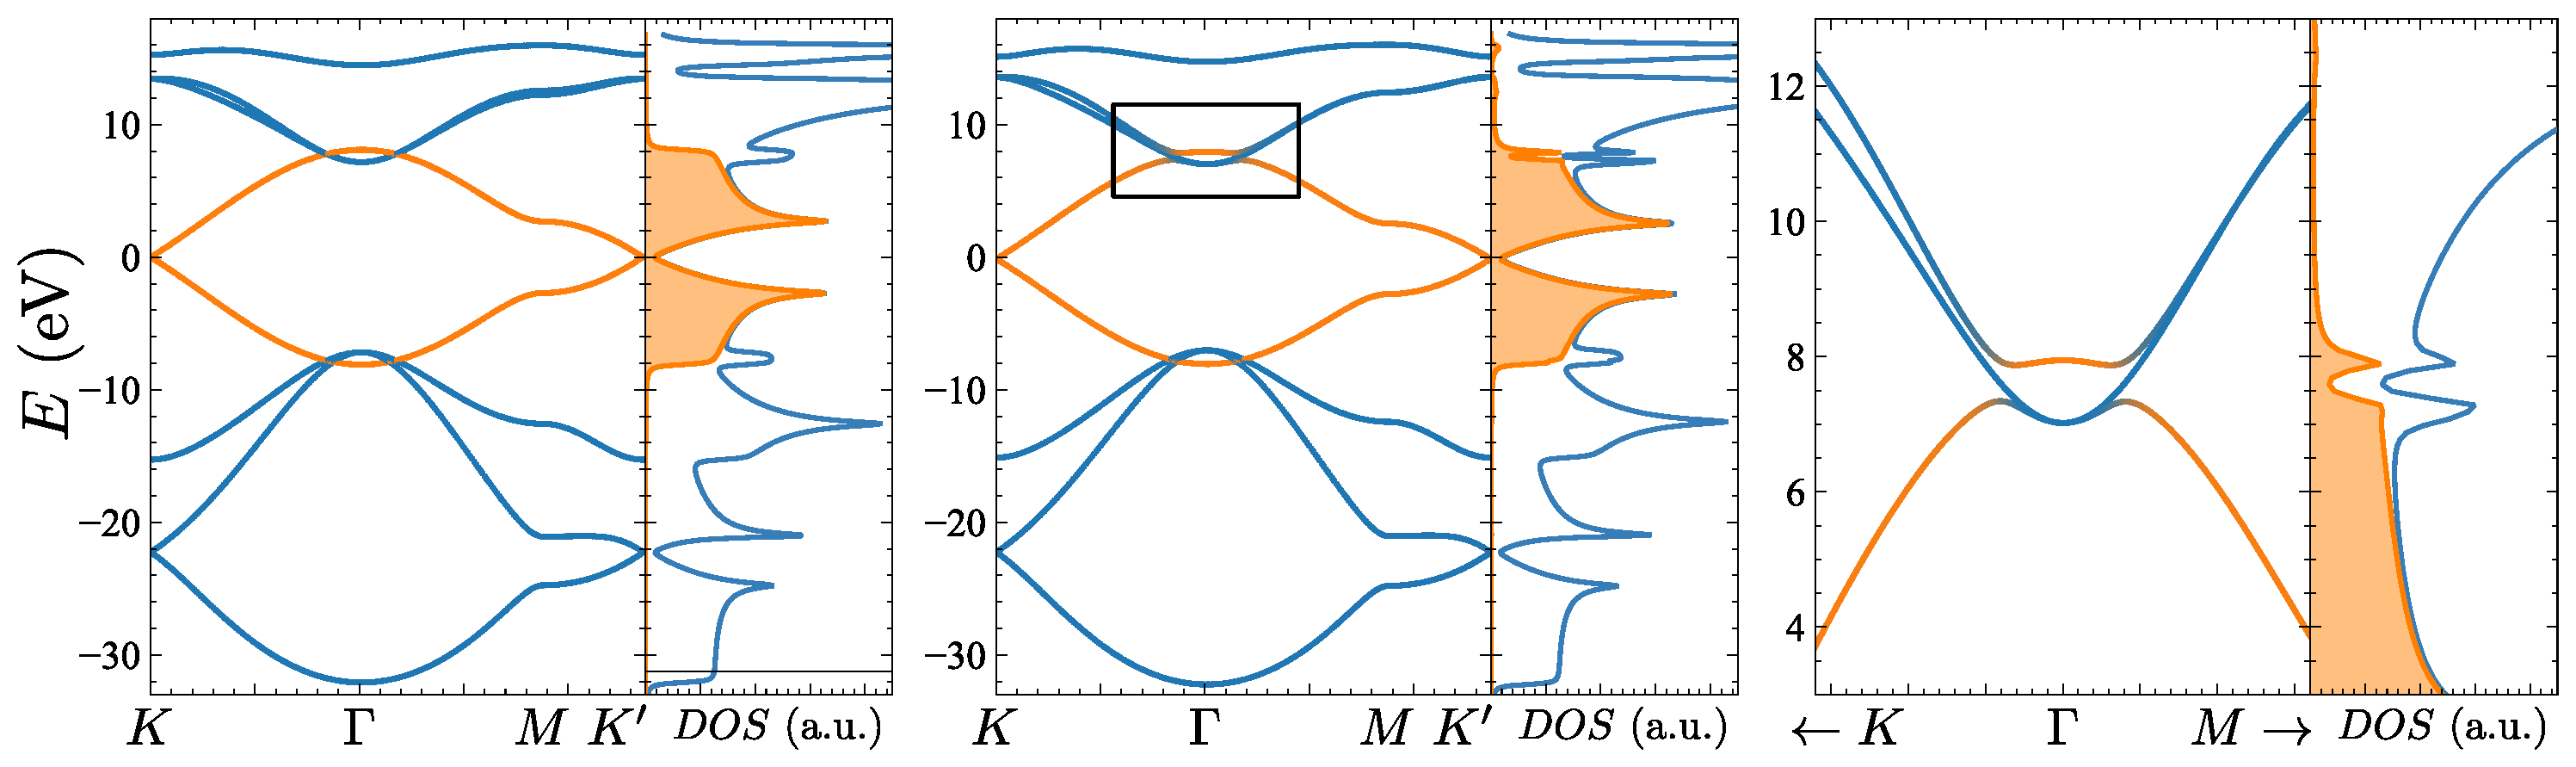
\includegraphics{graphene/figures/banddos_G_buck.pdf}
\vspace{-5pt}
\caption{a) Pristine graphene band structure and DOS. b) Buckled graphene band structure and DOS. c) zoom around the $\Gamma$ point where the $\sigma$-orbitals hybridize with the $\pi$-manifold.}
\label{fig:buckling}
\end{figure}
\FloatBarrier
%~~~~~~~~~~~~~~~~~~~~~~~~~~~~~~~~~~~~~~~~~~~~~~~~~~~~~~~~~~~%
This simple example shows how easy it is to account for geometric distortions using the \ac{sk} model. Notice that the buckling used in this example is quite similar to that naturally occurring in other materials such as 2-D Bismuth crystals.

\subsubsection{Other materials}
Once we have the machinery to build \ac{sk} hamiltonians, simply by changing the \ac{sk} parameters we can describe different materials.
In this section we compare graphene, bismuth and $h-\ce{BN}$  % TODO cite
as simple examples where the \ac{sk} description works well.\\

%
% Graphene TB
%
In order to describe \textbf{graphene}, different sets of parameters can be found in the literature\cite{Gosalbez-Martinez2011, Konschuh2010, Saito1998}. Nevertheless some of the parameters used here have been fitted from \ac{dft} calculations. The \ac{sk} parameters in $\si{\eV}$ used for graphene are:
\begin{equation}
  \begin{array}{l|cccc}
    Hopping & V_{ss\sigma} & V_{sp\sigma} & V_{pp\sigma} & V_{pp\pi} \\ \hline
    \ce{C}-\ce{C} & -7.76 & 8.16 & 7.48 & -2.7 \\
    \ce{C}-\ce{H} & -6.84 & 7.81 & \text{--} & \text{--}
  \end{array}\qquad\qquad
  \begin{array}{c|cccc}
    \text{On-site} & s & p_x & p_y & p_z \\ \hline
    \ce{C} & -8.8 & 0.0 & 0.0 & 0.0 \\
    \ce{H} & -2.5 &     &     &
  \end{array}
\label{G_SK_params}
\end{equation}
where the hoppings with a hypothetical $\ce{H}$ atom have been included for later convenience.
\medbreak

The description of $\pmb{h-\ce{BN}}$ is quite similar to that of graphene, it suffices to add a different on-site energy for the $\ce{B}$ and $\ce{N}$ atoms ($E_{\ce{B}} = -E_{\ce{N}}\sim\SI{3}{\eV}$) while keeping the inter-atomic hoppings similar to those of graphene\cite{Watanabe2004}.
\medbreak

\textbf{Bismuth} is a little bit more complex since an accurate description requires up to third neighbor hoppings (and spin-orbit coupling as well, which we will neglect for the moment). The \ac{sk} parameters, taken from~[\citen{Liu1995}] are:
\begin{equation}
  \begin{array}{c|cccc}
    Hopping & V_{ss\sigma} & V_{sp\sigma} & V_{pp\sigma} & V_{pp\pi} \\ \hline
    1 & -0.608 & 1.32 & 1.854 & -0.6 \\
    2 & -0.384 & 0.433 & 1.396 & -0.344 \\
    3 & \text{--} & \text{--} & 0.156 & \text{--}
  \end{array}\quad\qquad
  \begin{array}{c|cc}
     \text{On-site} & s & p_{x,y,z} \\ \hline
    \ce{Bi} & -10.906 & -0.486
  \end{array}
\label{Bi_SK_params}
\end{equation}
\medbreak

The respective band structure of all these materials is shown in \fref{SKbands}.
For all panels, the color, $\mathcal{C}$ represents the weight of the $p_z$ orbital in each state:
\begin{equation*}
   \mathcal{C}_\alpha = \bra{\psi_{\alpha}}\mathcal{O}_{p_z}\ket{\psi_{\alpha}}
\end{equation*}
where $\mathcal{O}_{p_z}$ is the $p_z$ projector operator and $\ket{\psi_{\alpha}}$ are the Hamiltonian eigenfunctions.
\begin{equation*}
  H\ket{\psi_{\alpha}} = E_{\alpha}\ket{\psi_{\alpha}} \qquad ; \qquad
   \ket{\psi} = \sum_i c_i\ket{\phi_i} \quad
   \text{for} \quad\ket{\phi_i}\in\mathcal{B}_4
\end{equation*}
%~~~~~~~~~~~~~~~~~~~~~~~~~~ FIGURE ~~~~~~~~~~~~~~~~~~~~~~~~~%
\begin{figure}[!ht]
\centering
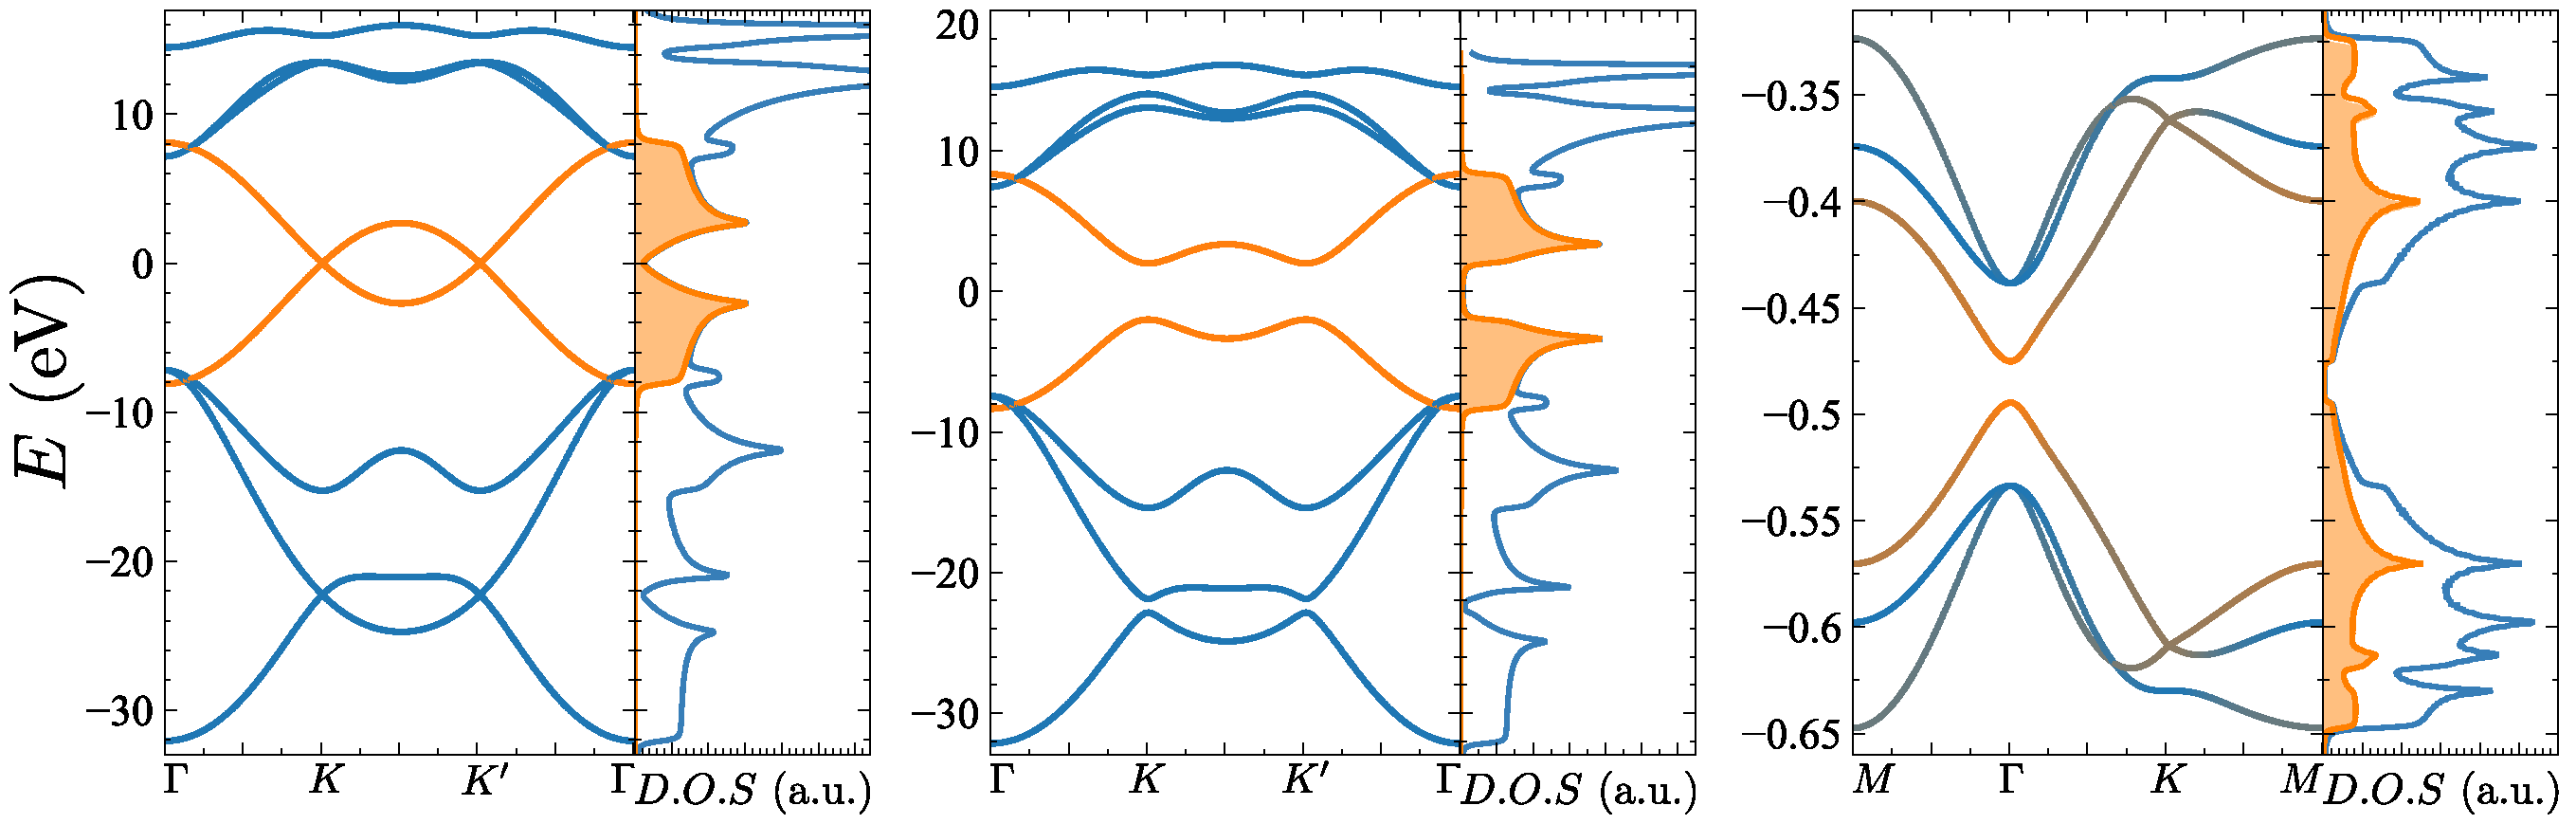
\includegraphics{graphene/figures/banddos.pdf}
\vspace{-15pt}
\caption{a) Graphene bands in the \ac{sk} approximation, with $s$, $p_x$, $p_y$, $p_z$ orbitals for the $\ce{C}$ atoms. The color denote the $p_z$ component of each state. It can be seen that the $p_z$ orbital are decoupled from the rest of the orbitals. b) $h-\ce{BN}$ band structure, similar to that of graphene, but with a gap open due to the difference in the on-site energies between the $\ce{B}$ and $\ce{N}$ atoms. c) Bismuth band structure, since its atomic structure is buckled, the $p_z$ orbital is not decoupled from the others as it can be seen by the smooth change in color of the central bands.}
\label{SKbands}
\end{figure}
\FloatBarrier
%~~~~~~~~~~~~~~~~~~~~~~~~~~~~~~~~~~~~~~~~~~~~~~~~~~~~~~~~~~~%

% TODO conclusion of SK?
These examples show that the \ac{sk} model provides a simple and versatile framework to capture a wide range of phenomena. It will be specially useful to capture structural deformations.


\section{Basic Properties}
\label{sec:graphene_basic_properties}
%
%  General description of bands
%  Low energy,
%
We are going to use a \ac{tb} model in the \ac{sk} approximation with four orbitals per carbon atom to describe graphene. The band structure obtained with this model is shown in \fref{bandsG}.

The first thing to notice about the graphene bands is the orbital distribution of the bands. As mentioned before, the $p_z$ orbitals are responsible for the central bands, crossing the Fermi energy ($E_F=\SI{0.0}{\eV}$). Due to the mirror symmetry of the system (with respect to the atomic plane), every hopping between the $\sigma$-orbitals and $p_z$ vanishes exactly (see the definition of $V_{sp\sigma}$ in \fref{orbitals}a)).
The presence of \textit{only} $p_z$ orbitals around the Fermi energy makes it possible to describe the system solely with these orbitals.

The second thing to notice is that around the Fermi level, the band dispersion is linear. In particular, the band structure forms two pairs of cones in the $K$ and $K'$ points of the \ac{fbz}. This famous feature, dubbed the Dirac Cones %TODO cite
is responsible for many of the interesting properties of graphene %TODO cite{Klein, HEP analogies, anomalies, topology,...}
%~~~~~~~~~~~~~~~~~~~~~~~~~~ FIGURE ~~~~~~~~~~~~~~~~~~~~~~~~~%
\begin{figure}[!ht]
\begin{center}
  %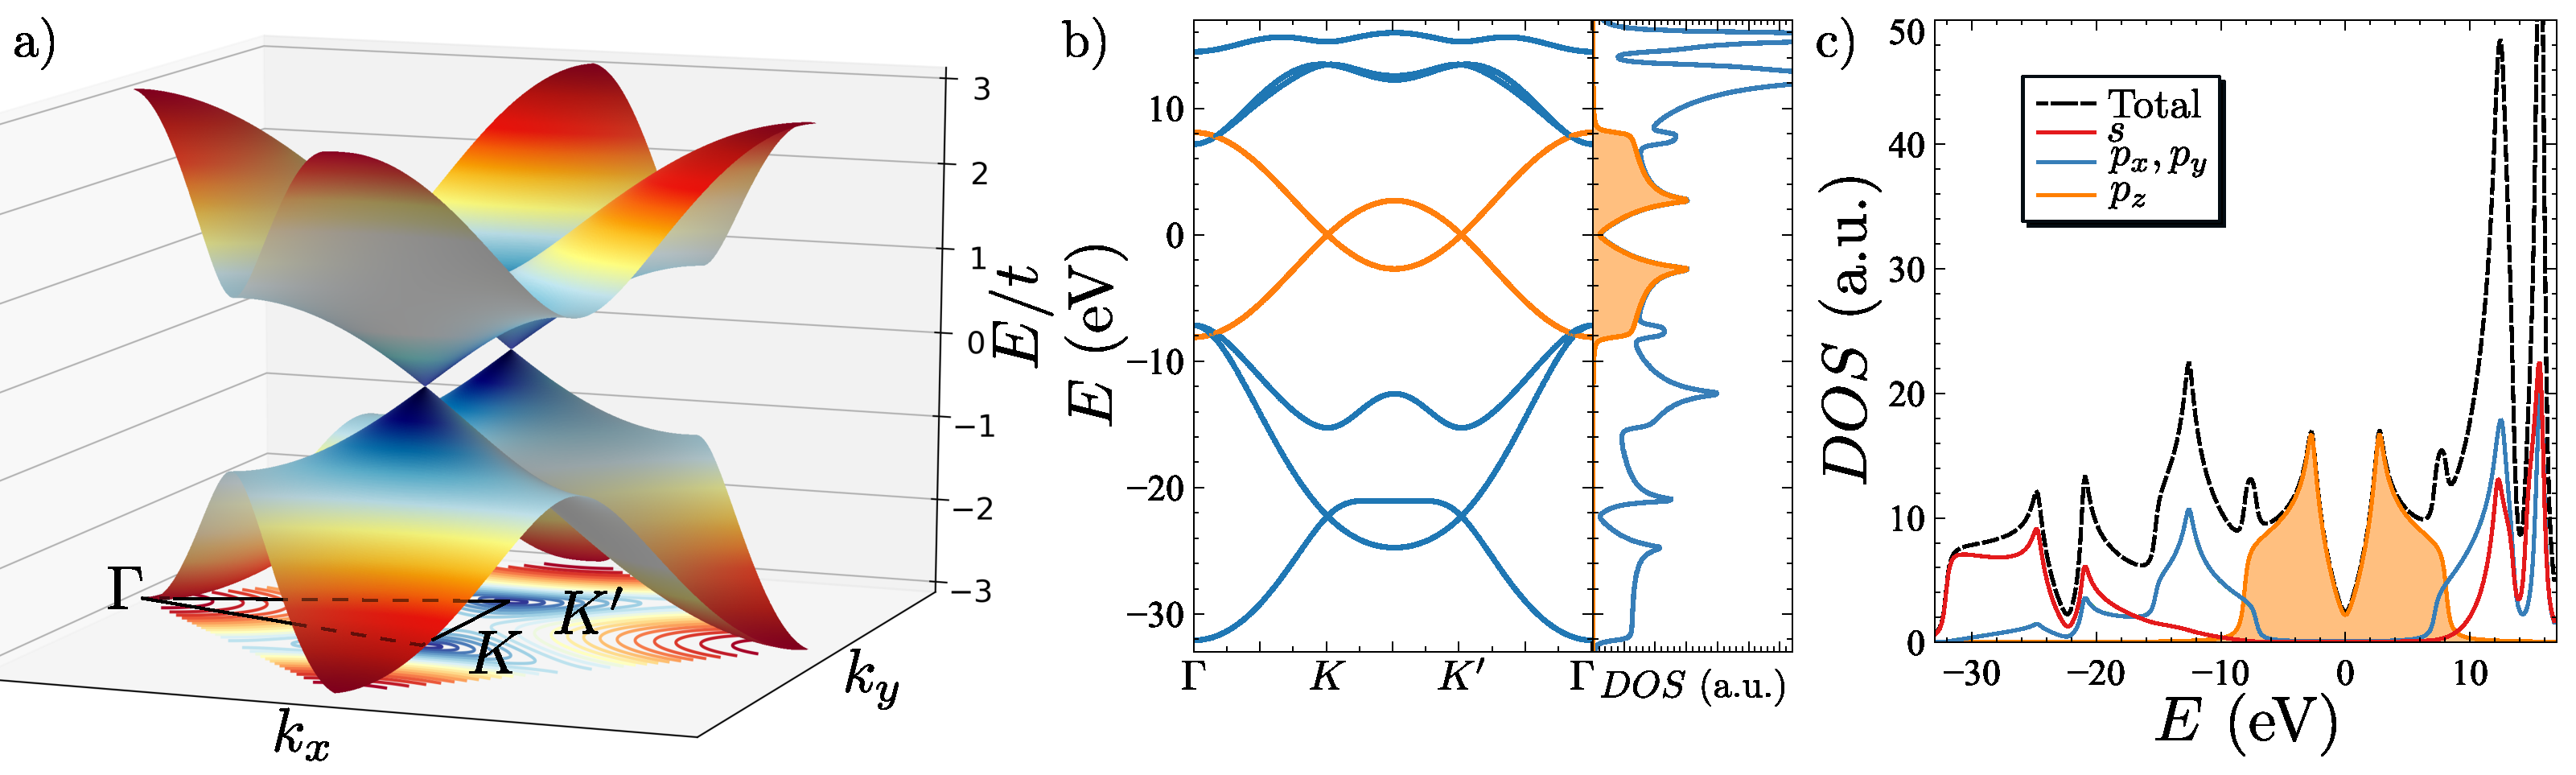
\includegraphics[width=1.1\textwidth]{graphene/figures/banddos_C.pdf}
  \makebox[\textwidth][c]{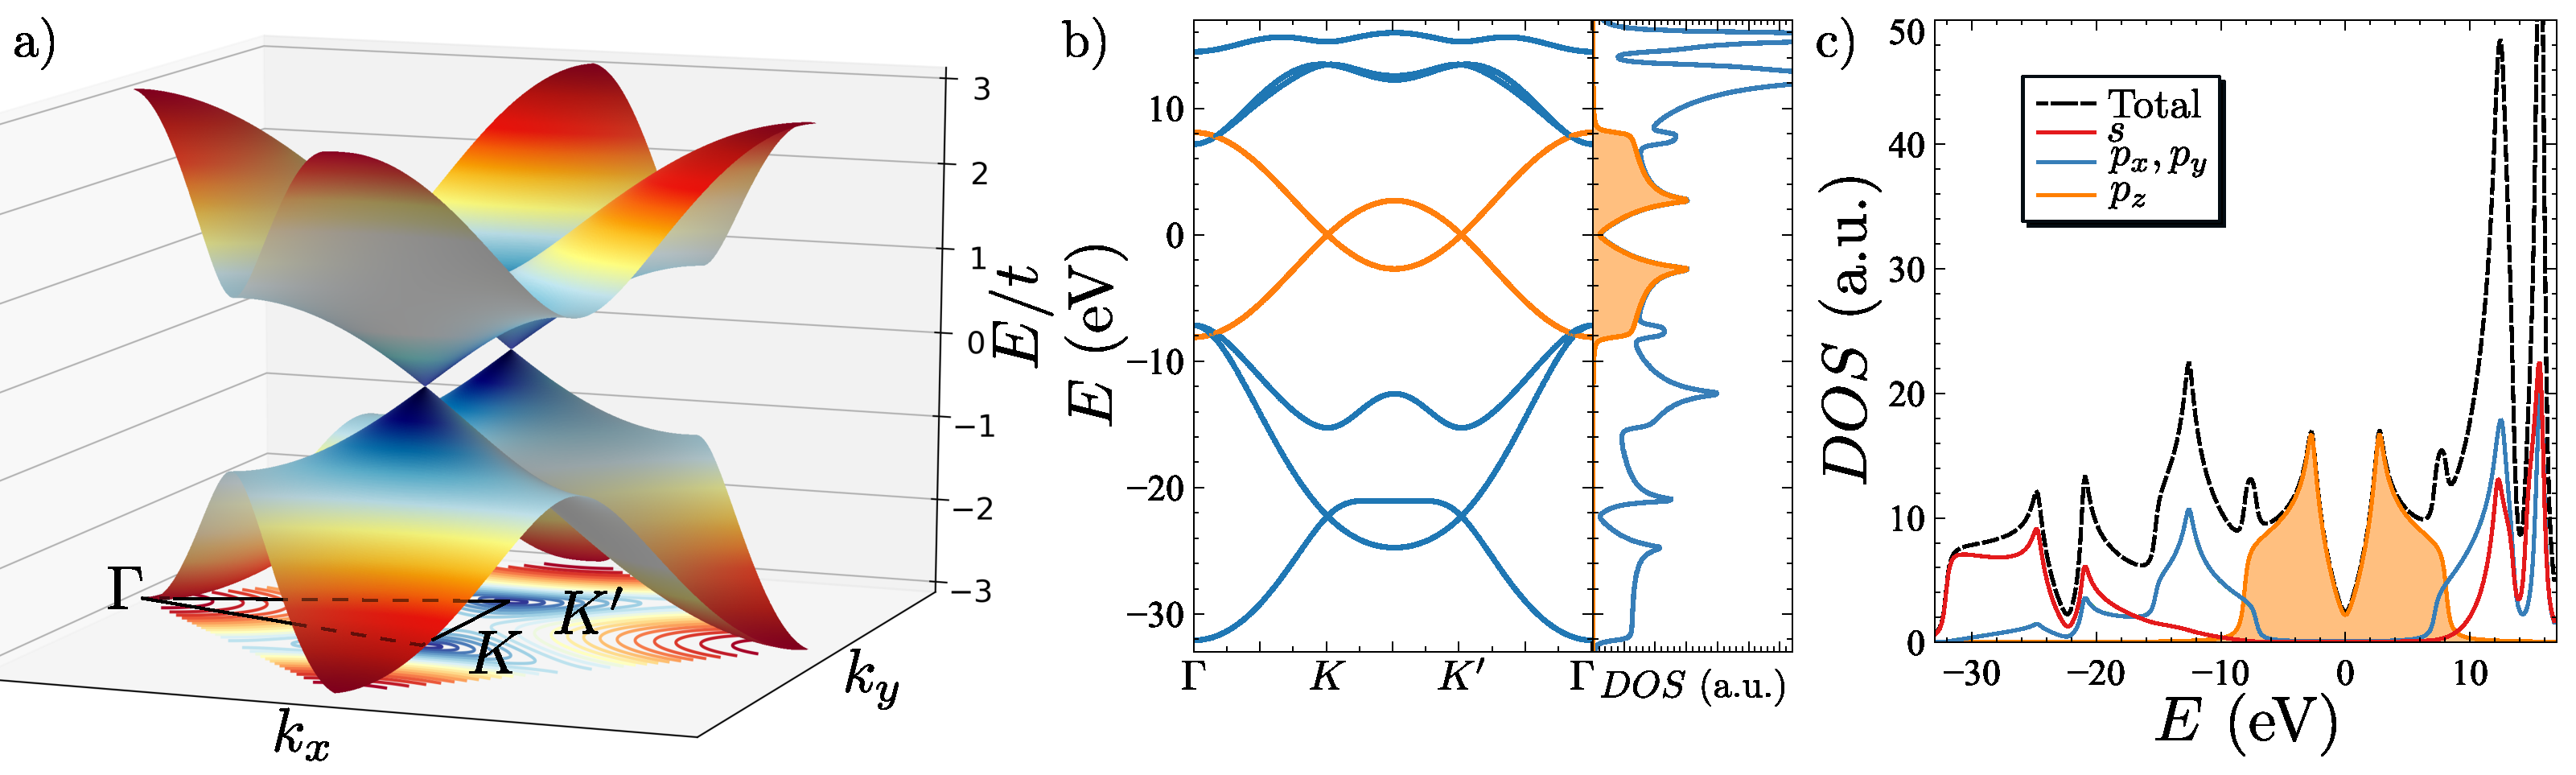
\includegraphics[width=1.2\textwidth]{graphene/figures/banddos_C.pdf}}
\end{center}
\vspace{-15pt}
\caption{a) 3D representation of the $p_z$ bands of graphene. Notice the two cones in the center of the FBZ. b) Band structure of graphene and DOS. b) DOS of graphene by orbital. Notice that the $p_x$ and $p_y$ contributions are degenerate.}
\label{bandsG}
\end{figure}
\FloatBarrier
%~~~~~~~~~~~~~~~~~~~~~~~~~~~~~~~~~~~~~~~~~~~~~~~~~~~~~~~~~~~%
In fact it is an easy exercise to calculate the band dispersion analytically. The Hamiltonian (already in the $k$-space) is:
\begin{equation}
   H(\vec{k}) = H_0 + V_1 e^{-i\vec{k}\vec{a}_1} + V_2 e^{-i\vec{k}\vec{a}_2}+
   V^{\dagger}_1 e^{i\vec{k}\vec{a}_1} + V^{\dagger}_2 e^{i\vec{k}\vec{a}_2}
\label{hk}
\end{equation}
where $\vec{a}_i$ are the lattice vectors described in \eqref{latt_vec} and, in the one orbital basis $\mathcal{B}_1$ described by \eqref{basis1}, can be written as
\begin{equation}
   H_0 = \left(\begin{array}{cc}
               \varepsilon_A & t \\
               t & \varepsilon_B
         \end{array}\right) \quad;\quad
   V_1 = V_2 = \left(\begin{array}{cc}
                     0 & 0 \\
                     t & 0
               \end{array}\right)
\end{equation}
which allows us to rewrite eq. \eqref{hk} as
\begin{equation}
  H(\vec{k})=\left(\begin{array}{cc}
        \varepsilon_{A} & tf(\vec{k}) \\
  tf^{\dagger}(\vec{k}) & \varepsilon_{B}
  \end{array}\right) \quad;\quad
  f(\vec{k}) = 1 + e^{-i\vec{k}\vec{a}_{1}}+
e^{-i\vec{k}\vec{a}_{2}}
\end{equation}
where we have assumed that the hopping integral between two coplanar $p_z$ orbitals is real. We have explicitly added a different on-site energy $\varepsilon_{A/B}$ for each of the sublattices

Finding the eigenvalues of $H(\vec{k})$ we obtain
\begin{equation}
  E(\vec{k})=\frac{\varepsilon_{B}-\varepsilon_{A}}{2}\pm
  \sqrt{\frac{\varepsilon^{2}_{A}+\varepsilon^{2}_{B}}{4}-
  \frac{\varepsilon_{A}\varepsilon_{B}}{2}-
  4\left(\varepsilon_{A}\varepsilon_{B}-
                                   t^2f(\vec{k})f^{\dagger}(\vec{k})\right) }
\end{equation}
yet in graphene these parameters vanish: $\varepsilon_{A}=\varepsilon_{B}=\varepsilon=0$ so the dispersion for the eigenvalues of the Hamiltonian:
\begin{equation}
  E(\vec{k})=\pm\sqrt{4t^2ff^{\dagger}} = \pm2|tf(\vec{k})|
\end{equation}

%
%
% XXX
% TODO Dirac derivation
%
%
%

\section{Other Terms in the Hamiltonian}
The Hamiltonian of graphene has been used as a toy model to describe many other materials since their Hamiltonian can be obtained as some modification of that of graphene. Here we explore some of the most commonly used Hamiltonian terms.

\subsection{Sublattice Imbalance}
If we were to consider not graphene but some other material with the same structure but different on-site energies for each sublattice, a so-called ``mass'' term would have to be introduced. This term appears in the description of $h-BN$ and even can be included in the proper description of graphene to account for some proximity effect.

The main effect of such a term is to open a trivial gap at the Dirac points as it was shown in the $h-BN$ bands \fref{SKbands}b).

\subsection{Zeeman}
Magntic field, $\vec{B}$, couples to both the spin and orbital degrees of freedom. Whereas orbital coupling leads to the formation of \ac{ll} when the field is perpendicular to the 2D material, in this thesis we do not address that situation, and only focus on the coupling ot the $\vec{B}$ field to the spin degree of freedom, the so called Zeeman interaction.

% The application of an external magnetic field usually has several effects in a material. While a lot of interesting Physics is developed around the formation of Landau levels\cite{}, %TODO
% We will restrict our study to the simpler case of the Zeeman splitting of the energy levels.
 
This effect consists of a symmetric splitting of up ($\uaw$) and down ($\daw$) spins, resulting in a opposed energy shift of the bands for each spin flavor. %TODO figure

\subsection{Spin-Orbit coupling}
\label{sec:soc}
The \acf{soc} is a relativistic effect that can be interpreted in classical terms (allowing the existence of spin in classical physics) as the interaction between the spin of the electron and the electrostatic potential of the nucleus.

In most of this section we are going to use the four orbital basis \eqref{basis4} with the geometry of \fref{graphene_summary}b), also described in the first section of the chapter.
In this basis there are two atoms per unit cell and four orbitals per atom, so our Hamiltonian would be a $8\times8$ matrix. When interactions concerning the spin are taken into account, the basis needs to be doubled and we choose the following order to do so:
\begin{equation}
  \mathcal{B}^{s}_4 = \left\{
  \ket{\phi^1_{s\uaw}},
  \ket{\phi^1_{s\daw}},
  \ket{\phi^1_{p_x\uaw}},
  \ket{\phi^1_{p_x\daw}},
  \ket{\phi^1_{p_y\uaw}},
  \ket{\phi^1_{p_y\daw}},
  \dots,
  \ket{\phi^n_{p_z\uaw}},
  \ket{\phi^n_{p_z\daw}}
  \right\}
\label{basis4spin}
\end{equation}

So the \ac{soc} Hamiltonian term can be written as follows:
\begin{equation}
   H_{SO}= \lambda_{SO}\vec{L}\cdot\vec{S} =
   \lambda_{SO}\left[L_xS_x + L_yS_y + L_zS_z \right] =
   \lambda_{SO}\left[L_zS_z+
   \frac{1}{2}\left(L^{+}S^{-}+L^{-}S^{+}\right)\right]
\label{soc}
\end{equation}
just by taking into account the relations
\begin{equation*}
   S^{+} = S_x + iS_y \quad;\quad
   S^{-} = S_x - iS_y
\end{equation*}

%~~~~~~~~~~~~~~~~~~~~~~~~~~ FIGURE ~~~~~~~~~~~~~~~~~~~~~~~~~%
\begin{figure}[!ht]
\centering
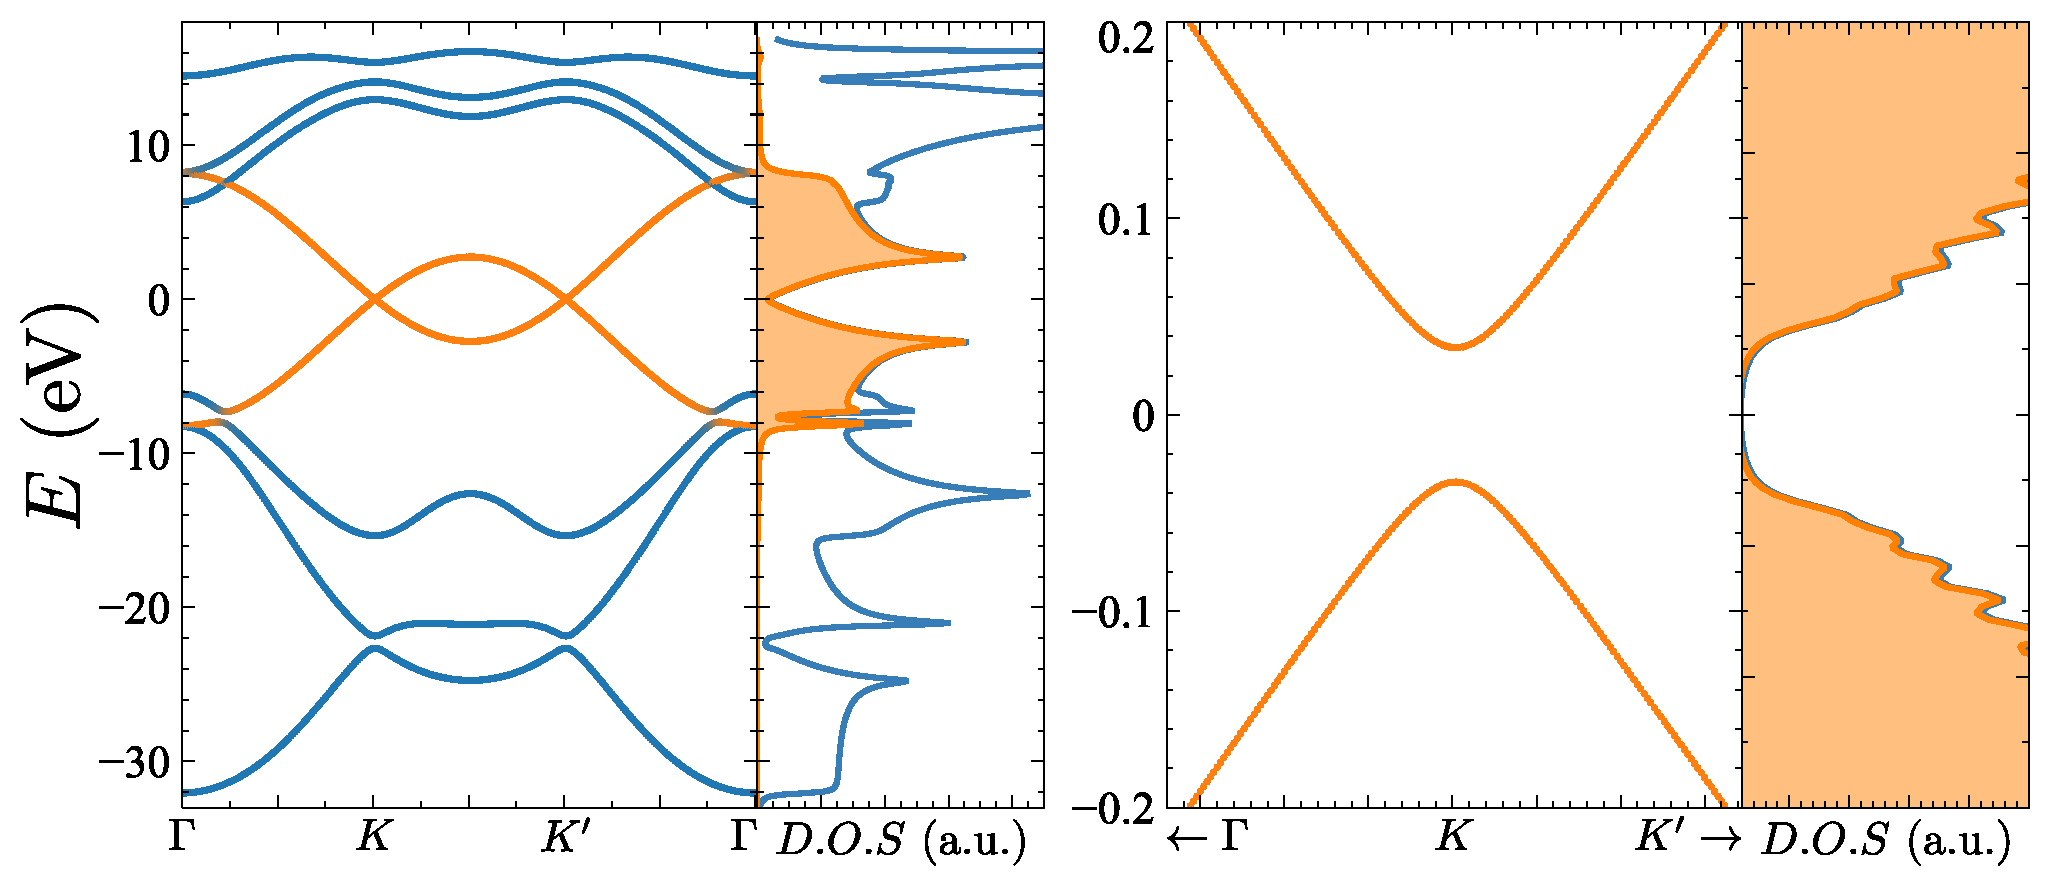
\includegraphics{graphene/figures/banddos_SOC.pdf}
\vspace{-5pt}
\caption{a) Graphene band structure in the presence of \ac{soc}. The gap due to \ac{soc} is not visible at this scale but the mixing of the $p_z$ orbital with the $\sigma$-bands becomes apparent near $\Gamma$. b) Zoom for $E$ close to the Dirac point. A gap is open in the band structure turning graphene into a topological insulator. The spikes in the DOS are just an artifact of the calculation due, mainly, to the limited precision in the k-space integration.}
\label{fig:SOC}
\end{figure}
\FloatBarrier
%~~~~~~~~~~~~~~~~~~~~~~~~~~~~~~~~~~~~~~~~~~~~~~~~~~~~~~~~~~~%

This term is responsible for the opening of a band gap at the $K$ points turning graphene into a \ac{ti}. %TODO cite
This term is known to be equivalent to having a second neighbor imaginary hopping in the $p_z$ manifold\cite{Haldane1988,Kane2005,Kane2005a}. This term induces a non-trivial Berry phase which gives rise to its topological behavior.
This term is at the core of the \ac{qsh} effect. % observed in experiment.


\subsection{Electric field and Rashba}  %XXX REVIEW
An electric field has several effects that will be discussed extensively along the thesis. It should suffice for now to discuss briefly the orbital consequences.
When an external electric field perpendicular to the material is applied the atomic orbitals get deformed, breaking the mirror symmetry that protects the $\pi$-manifold. The breaking of this symmetry opens an effective hopping channel for mixing $s$ and $p_z$ orbitals.

Another effect, alongside the \ac{soc}, is the appearance of a spin-flip channel via the following process: an $\uaw$ electron in a $p_z$ can transition to a $s$ orbital in the same atom via rashba hopping, then to a $p_{x/y}$ orbital centered in a neighboring atom, which is connected via \ac{soc} with a $p_z$ with spin $\daw$.

Following the calculations in \cite{Min2006} we can see that the relation between the applied electric field and the effective intra-atomic Rashba follow the equation:
\begin{equation}
   \lambda_R=\frac{e\mathcal{E}z_0}{3V_{sp\sigma}}\xi \qquad;\qquad
   \lambda_{SOC}=\frac{|E_{s}|}{18V^2_{sp\sigma}}\xi^2
% \label{rashba}
\end{equation}
where $\xi\sim\SI{6}{\meV}$ is the atomic carbon spin-orbit coupling strength
which for a typical electric field of $\mathcal{E}\sim\SI{50}{\V}/\SI{300}{\nm}$ result in an effective Rashba coupling $\lambda_R\sim\SI{0.011}{\meV}$ and the \ac{soc} $\lambda_{SOC}\sim\SI{0.0011}{\meV}$.

These terms, are in the scale of $\SI{e-2}{\meV}$ while the gap open can reach up to $\SI{2.5e2}{\meV}$ so we will neglect these interactions from now on.
\bigskip


If we consider bilayer graphene, the application of an electric field has another important effect. It shifts the on-site energy of each layer which results in an opening of a gap in the band structure. This results in a very useful feature that will be exploited throughout the thesis.





%\section{Graphene Bilayer}
%\label{ch:bilayer}
%Graphite is made out of weakly bounded graphene layers, which is one of the reasons why exfoliating it is relatively easy. Extensive work has been devoted to systems in which two layers are isolated\cite{McCann2012}.
%
%The description is not much different from that of graphene: the Bravais lattice is still a triangular lattice with lattice vectors described by \eqref{latt_vec}, hence the \ac{fbz} is the same. The main difference is that the minimal basis now has four atomic positions.
%%~~~~~~~~~~~~~~~~~~~~~~~~~~ FIGURE ~~~~~~~~~~~~~~~~~~~~~~~~~%
%\begin{figure}[!ht]
%\centering
%\includegraphics{graphene/figures/graphene_bi_summary.pdf}
%\vspace{-5pt}
%\caption{a) Cartoon depiction of the atomic structure of bilayer graphene using the lattice vectors defined in \eqref{latt_vec}. b) Band structure of bilayer graphene. Notice the c) Comparison of the band structure and \ac{dos} in the presence of an external electric field.}
%\label{Gbi_summary}
%\end{figure}
%\FloatBarrier
%%~~~~~~~~~~~~~~~~~~~~~~~~~~~~~~~~~~~~~~~~~~~~~~~~~~~~~~~~~~~%
%In bilayer graphene the $p_z$ manifold is no longer decoupled from the other orbitals since there are hopping processes between the $p_z$ orbitals in one layer and the $s$ orbitals in the other layer. Nevertheless the $p_x$ and $p_y$ still have no direct hopping with the $p_z$ orbitals.
%While it is true that the symmetry protecting the $p_z$ manifold is broken in this system, the fact remains that at low energy and around the $K$ points the $p_z$ description is enough (and exactly at the Dirac points it is an exact description).\\
%
%There are several ways in which we can stack several graphene layers. Until further notice we will consider only Bernal stacking, meaning that only one of the sublattices of one layer is connected to the opposite sublattice of the other layer. This configuration results in having in each layer one sublattice which is ``\emph{connected}'' and another that lays on ``\emph{hollow}'' sites (\fref{Gbi_summary}{a)}).
%
%We can approach bilayer graphene by considering two decoupled layers of graphene. In this case we would have twice the typical graphene band structure, one for each layer. When the interlayer coupling is switched on (see \eqref{Gbi}) two of the bands split from the rest according to the interlayer hopping $t'$ and the other two become parabolic.\\
%
%
%
%\subsection{electric field}
%It is well known that the band structure of bilayer graphene changes dramatically in the presence of an external electric field\cite{Oostinga2007, Zhang2009, Taychatanapat2010, Allen2012, Castro2010a, Ponomarenko2011, Sui2015}.
%The application of an electric field has several effects in the electronic structure of the system.
%
%The most obvious effect is the different shift of the on-site energies for each layer. This effect breaks the bipartite-ness of the system and results in a tunable band gap as reported by many experiments.
%
%Another effect is the possible doping of the system. By simply gating bilayer graphene we would be introducing a lot of carriers resulting in huge filling factors. This problem/feature can be address and, in fact used to our advantage by using dual-gating rather than a single gate as we will see in the following sections.
%
%Finally, the last effect is the appearance of a Rashba-like term due to the deformation of the atomic orbitals which could open both $s-p_z$ hoppings and a spin flip channel (when combined with the \ac{soc}).
%
%
%\subsubsection{Gap opening}
%The effect of an electric field in the electronic structure is just a layer dependent shift in the on-site energies of the atomic orbitals. In particular, in the basis \eqref{basis_bi}, it can be written as
%\begin{equation}
%   H_\mathcal{E} = \mathcal{E}\Lambda = \left(
%   \begin{array}{cc|cc}
%     \mathcal{E} & 0 & 0 & 0\\
%     0 & \mathcal{E} & 0 & 0\\ \hline
%     0 & 0 & -\mathcal{E} & 0\\
%     0 & 0 & 0 & -\mathcal{E}\\
%   \end{array}\right)
%\label{Helec}
%\end{equation}
%where $\Lambda$ is the layer operator and $\mathcal{E}$ the strength of the electric field.
%
%In particular, a band gap is open at the Dirac points as shown in \fref{Gbi_summary}{c)}. Along with this effect, there are other processes not captured by the model, for instance a strong redistribution of the charge will take place in the system, polarizing the two layers in opposition to the applied electric field. This screening process has be addressed in the literature showing that its main effect is a Hartree renormalization of the gap\cite{McCann2006,Wang2016a}. While this effects are certainly not negligible we can adopt an empirical approach based on the experimental observation\cite{Zhang2009, Taychatanapat2010} of a gap up to $\Delta=\SI{250}{\meV}$, regardless of the real voltage required to achieve it.
%
%
%
%\subsubsection{Doping}
%%~~~~~~~~~~~~~~~~~~~~~~~~~~ FIGURE ~~~~~~~~~~~~~~~~~~~~~~~~~%
%\begin{figure}[!ht]
%\centering
%\includegraphics[width=0.5\textwidth]{graphene/figures/dual_gate.pdf}
%\vspace{-5pt}
%\caption{Schematics of dual gating.}
%\label{dual_gate}
%\end{figure}
%\FloatBarrier
%%~~~~~~~~~~~~~~~~~~~~~~~~~~~~~~~~~~~~~~~~~~~~~~~~~~~~~~~~~~~%
%The doping (extra charge absorbed into the system) in the graphene bilayer can  be estimated simply by applying Gauss' law:
%\begin{equation}
%   \diver{D} = \rho-\rho_0 = \rho_f
%\label{gauss}
%\end{equation}
%where $\rho$ is total charge density, $\rho_0$ is the bounded charge density so that $\rho_f$ is the free charge density.
%
%The dual-gating setup can be considered as an infinite capacitor, hence, the electric field only has $z$ component, hence the divergence of the displacement results in a derivative which can be discretized:
%\begin{equation}
%   \diver{D}=\frac{\partial D}{\partial z} =\frac{D_t-D_b}{dz} = \rho_f =
%   e\frac{N}{V} \Rightarrow D_t-D_b = e\delta n
%\label{doping}
%\end{equation}
%where $N$ and $V=Adz$ are the number of electrons and volume respectively ($A$ is the area), and $\delta n$ is the bidimensional density of electrons.
%
%In order to calculate the potential difference between the two graphene layers, we can consider simply the average of the electric field inside the capacitor:
%\begin{equation}
%   \Delta V = \langle\vec{E}\rangle \Delta z = \frac{E_t+E_b}{2} \Delta z=
%   \frac{\Delta z}{2} \left(\frac{D_t}{\varepsilon_t} +
%                            \frac{D_b}{\varepsilon_b} \right)
%\label{potential}
%\end{equation}
%where $\Delta z$ is width of the graphene bilayer and $\varepsilon_t$ and       $\varepsilon_b$ are the electric permeability of the top and bottom             dielectrics. $D_t$ and $D_b$ are (the $z$-component of) the displacement fields in the top and bottom regions.
%\begin{equation}
%   D_t = \frac{\varepsilon_t}{d_t}\left(V_{t}-V^0_{t}\right) \qquad;\qquad
%   D_b = \frac{\varepsilon_b}{d_b}\left(V_{b}-V^0_{b}\right)
%\end{equation}
%where $V^0_{t/b}$ are the off-set potential required to have charge neutrality, usually referred to as \ac{cnp}.
%
%Equations \eqref{doping} and \eqref{potential} show that by choosing the        appropriates $V_t$ and $V_b$ we can independently change the doping of the      system and the gap opened in the band structure.
%
%
%
%
%
%\subsubsection{Rashba}
%Another effect is the mixing of the $p_z$ with the other orbitals. The presence of the electric field deforms the atomic orbitals breaking the symmetries present in the purely hydrogenic orbitals. In particular a new intra-atomic hopping $p_z$ and the $p_{x/y}$ orbitals appear. The application of an electric field leads to the appearance of an intrinsic Rashba and \ac{soc} similar to the terms proposed by Kane and Mele\cite{Kane2005}.
%Following the calculations in \citef{Min2006}\cite{Min2006} we can see that the relation between the applied electric field and the effective intra-atomic Rashba follow the equation:
%\begin{equation}
%   \lambda_R=\frac{e\mathcal{E}z_0}{3V_{sp\sigma}}\xi \qquad;\qquad
%   \lambda_{SOC}=\frac{|E_{s}|}{18V^2_{sp\sigma}}\xi^2
%\label{rashba}
%\end{equation}
%where $\xi\sim\SI{6}{\meV}$ is the atomic carbon spin-orbit coupling strength
%which for a typical electric field of $\mathcal{E}\sim\SI{50}{\V}/\SI{300}{\nm}$ result in an effective Rashba coupling $\lambda_R\sim\SI{0.011}{\meV}$ and the \ac{soc} $\lambda_{SOC}\sim\SI{0.0011}{\meV}$.
%
%These terms, are in the scale of $\SI{e-2}{\meV}$ while the gap open can reach up to $\SI{2.5e2}{\meV}$ so we will neglect these interactions from now on.
%

%\chapter{Real space mapping of topological invariants using artificial neural networks}

\section{Introduction}
The study of topological electronic phases is one of the central topics %themes
in modern Condensed Matter Physics. Depending on the symmetry class different
topological states exist, with the paradigmatic examples of
time reversal topological insulators,\cite{RevModPhys.82.3045}
topological superconductors,\cite{RevModPhys.83.1057}
topological crystal insulators,\cite{PhysRevLett.106.106802}
topological Kondo insulators\cite{PhysRevLett.104.106408} and
topological Mott insulators\cite{PhysRevLett.100.156401} among others.
The most fundamental quantity to characterize these states is the so called
topological invariant, whose value determines the topological class of the
system.
In particular, interfaces between systems with different topological invariants
show topologically protected excitations, resilient towards perturbations
respecting the symmetry class of the system.
Computationally, the calculation of the topological invariant usually requires
the explicit knowledge of the wavefunctions of the entire 
system.\cite{PhysRevB.83.235401,PhysRevB.95.075146,wu2017wanniertools}
In particular,
topological invariants can
be calculated as the winding number of the 
occupied wave functions 
under
twisted boundary
conditions.\cite{PhysRevB.83.235401,PhysRevB.95.075146,wu2017wanniertools}
In that way, these methods generically require computing the full
wavefunctions, that becomes a cumbersome task for
systems without translational symmetry consisting on thousands
of atoms.


In several situations of experimental relevance, translational symmetry is
broken and systems are able to show different phases in real space due to the
spatial modulation of the effective parameters.
This situation might lead to protected modes between different regions of the
system, dramatically changing the low energy properties of the whole material.
This is the natural scenario in van der Waals heterostructures, where Moire
patterns\cite{PhysRevB.90.075428,PhysRevB.96.085442,wang2016gaps} could coexist
with any topological state.\cite{sanchez2017helical,Young2014}
A more controlled situation is the proposals for topological superconductivity
involving nanowires, where the topological state is controlled \emph{locally} by
electric gates.\cite{Alicea2011,Gul20168}
Even though real space formulations for the topological invariant do
exist,\cite{PhysRevB.84.241106,PhysRevB.95.121114,loring2015k,mitchell2018amorphous,fulga2016aperiodic} their computation requires an
integration over the whole space. Thus,  there is not a simple
methodology to obtain a topological invariant  in inhomogeneus systems by
evaluating solely their local properties.


Application of Machine learning methods in Condensed Matter Physics
is a growing area.
A significant advantage of these techniques is that they are capable of finding the
important degrees of freedom of a dataset without needing a profound insight of
the treated problem.
The identification of phase transitions\cite{VanNieuwenburg2017,PhysRevX.7.031038,ohtsuki2016deep,PhysRevE.95.062122,broecker2017quantum,koch2017mutual}
and the study of the ground state and correlations in different quantum many
body
problems\cite{carleo2017solving,deng2016exact,PhysRevX.7.021021,PhysRevLett.118.216401,nagai2017self,PhysRevE.97.013306}
are just some of the problems that Machine Learning has helped tackle in the
past few years. Even some techniques have been used in combination with
\textit{ab initio} calculations allowing a broader and more accurate
understanding of
materials.\cite{PhysRevLett.108.058301,bartok2017machine,gao2016machine}
% Thus, our goal will be to borrow tools from machine learning to compute the
% topological invariant of a system based only on real space information.
Within the language of machine learning, the calculation of topological
invariants is understood as a simple classification algorithm,\cite{PhysRevLett.120.066401,yoshioka2017learning}
that could be
efficiently tackled with the so called artificial neural networks.
\cite{alexnet2012,Dede20107,Lecun1998,Goldberg2015,Bengio2003,pybrain2010jmlr}


In this manuscript we show that artificial neural networks (ANN) are capable of
characterizing the local topology of a system using as input a restricted amount
of real space information.
In particular, we show that a trained ANN identifies correctly the local
topological character in spatially varying Hamiltonians that create
topologically different regions in space.
Importantly, we show that this technique, used in conjunction with the kernel
polynomial method, allows to compute local topological invariants with
an algorithm whose computational cost scales just linearly with the size of the
system.

The rest of the paper is organized as follows. In section~\ref{sec:met} we
review the basics of artificial neural networks (Sec.~\ref{sec:NN}) and
summarize the use of the kernel polynomial method to efficiently compute density
matrices (Sec.~\ref{sec:KPM}).
In section~\ref{sec:Topo} we apply the combined ANN-KPM technique both to a
model Hamiltonian for a 1-D topological superconductor (Sec.~\ref{sec:1d}) and a
2-D anomalous Hall insulator (Sec.~\ref{sec:2d}). Finally, in
section~\ref{sec:Conc} we present our conclusions.




\section{Method}
\label{sec:met}
%%%%%%%%%%%%%%%%%%%%%%%%%%%%%%%%%%%%%%%%%%%%%%%%%%%%%%%%%%%%%%%%%%%%%%%%%%%%%%%%
\subsection{Artificial Neural Networks}
\label{sec:NN}
Machine Learning (ML) is a broad field that includes many different approaches,
goals and methods.\cite{Solomonoff1957}
The defining property of ML algorithms is that they allow computers to perform
specific tasks without being explicitly programmed for each one of
them.\cite{Samuel1959} Within the vast variety of ML algorithms, we will focus
on supervised learning algorithms, which require a training dataset to fit the
parameters in the model. One of the most common models of supervised learning are
\emph{Artificial Neural Networks} (ANN) which have been proven very useful to
model patterns and correlations of complex problems that cannot be modeled
analytically such as image or sound
recognition,\cite{alexnet2012,Dede20107,Lecun1998} and even natural language
processing.\cite{Goldberg2015,Bengio2003}
In our case, we aim to use an artificial neural network to characterize
locally the topological state of a one (Fig.~\ref{fig1}~(a)) or two
(Fig.~\ref{fig1}~(b)) dimensional system. The objective of the procedure
is to have a neural network that, given local information about the system,
returns the topological invariant as sketched in Fig.~\ref{fig1}~(c).
The local information that will be provided is a local block of the density
matrix of the system, as we will discuss later.

%~~~~~~~~~~~~~~~~~~~~~~~~~~ FIGURE ~~~~~~~~~~~~~~~~~~~~~~~~~%
\begin{figure}[ht!]
\centering
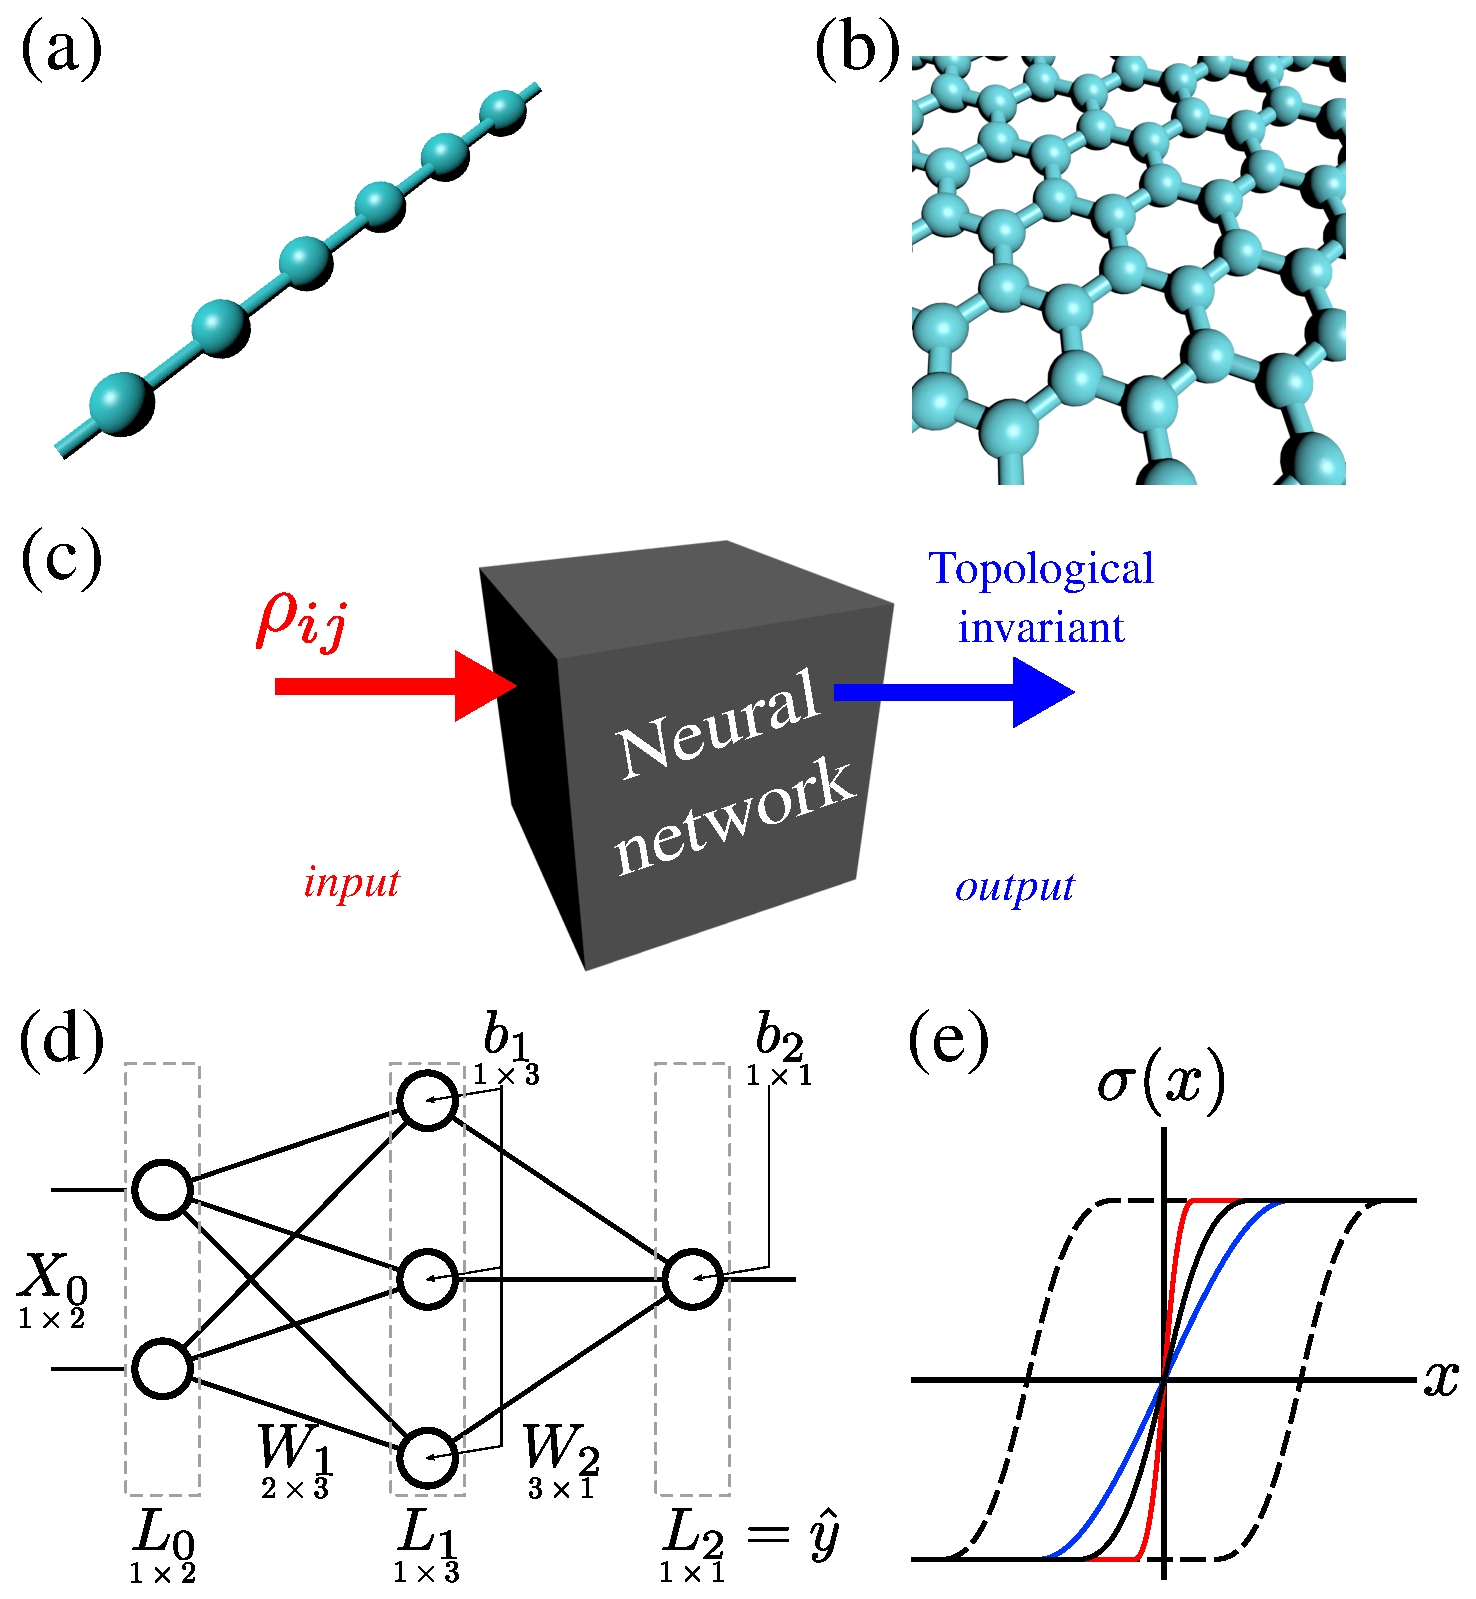
\includegraphics[width=0.5\textwidth]{ann/figures/fig1.pdf}
\vspace{-5pt}
\caption{
Panels (a,b) show a cartoon of the two different geometries of the model Hamiltonians considered  below, 
%systems that we aim to topologically characterized.
a one dimensional topological superconductor  (a) and a two dimensional  quantum anomalous Hall insulator (b).
Panel (c) shows a schematic sketch of our procedure: a trained neural network
will take as input a local density matrix, and it will return the topological
invariant of the system.
Panel (d) shows a sketch for an artificial neural network as described in the text, whereas
in (e) we sketch the standard behavior of an activation function of a neuron,
$\sigma(x)$, for different weights (colors) and bias (dashed lines).
}
\label{ANN}
\label{fig1}
\end{figure}
%~~~~~~~~~~~~~~~~~~~~~~~~~~~~~~~~~~~~~~~~~~~~~~~~~~~~~~~~~~~%

ANN are loosely based on parts of the brain, consisting of neurons, modeled as
perceptrons\cite{Rosenblatt1958}, and synapses as shown in Fig.~\ref{ANN}~(a).
%\buemark{Every neuron in an ANN has a number of inputs and outputs in the form of real numbers}
The neurons in an ANN do not attempt to model the actual structure or behavior
of the biological cells\cite{Hodgkin1952}. Instead, they mimic one of their main
features, the activation function.
This activation function, $\sigma$, sketched in Fig.~\ref{ANN}~(b) provides the
output of each neuron based on the received inputs and an external parameter
(bias). For computational convenience, $\sigma$ should be any smooth and
differentiable function defined over $\mathbb{R}$ but with its range restricted
to a closed interval, namely $\sigma\in[-1,1]$, as depicted in Fig.~\ref{ANN}~(e).
Usually, these functions are either the $\tanh$ or the sigmoid function, but
others might be used without loss of generality or functionality since these
models are only weakly sensitive to these details.\cite{Hopfield1982}


The inputs $X$ entering each neuron are weighted by the synapses $W$ and shifted
by the bias $b$. The synapses' weights are parameters to be tuned and they can be
arranged as rectangular matrices, $W^{\alpha}$, so the output
$L$ of the layer $\alpha$ can be obtained simply as:
$L_\alpha=\sigma(X_\alpha\cdot W_\alpha + b_\alpha)$,
where $X_\alpha$ is the input of the layer $\alpha$ (note that for the hidden
layers $X_\alpha=L_{\alpha-1}$).
As a formative example the outputs of every layer of the toy model sketched in
Fig.~\ref{ANN}~(d) can be calculated as follows:
\begin{equation}
  \begin{split}
    L_0 &= \sigma(X_0) \quad\text{or just}\quad L_0 = X_0 \\
    L_1 &= \sigma\left(L_0 \cdot W_1 + b_1\right) \\
    L_2 &= \sigma\left(L_1\cdot W_2 + b_2\right)= \hat{y}
  \end{split}
\label{FF}
\end{equation}
where $X_0$ is the input fed to the ANN.
The matrices $W_\alpha$ and the arrays $b_\alpha$ are the parameters to be
fitted during the training process in order to modify the activation functions
of each of the neurons in the ways showed in Fig.~\ref{ANN}~(e). Note that the
number of parameters in ANN models grows very quickly with the size (number of
neurons per layer) and depth (number of layers) of the network.\\


%In our case, we will employ ANN to implement a supervised
%learning algorithm. This kind of algorithms consist in three phases.
Artificial neural network, as every supervised learning algorithm, consist in
three phases.
First, the architecture of the model (i.e. the number of layers and neurons per
layer) is decided depending on the complexity of the problem addressed.
Second, the model is trained. In this process, several input-output pairs are
provided to the model whose parameters are fitted to mimic the correlations
present in the user-provided data.
Finally, when the training is completed, the model can be used to evaluate new
(unseen) input data.


Supervised learning algorithms require a training dataset to optimize the
parameters of the models. The training is performed by minimizing a cost
function, $\mathcal{E}$, usually proportional to the squared difference between
the expected output, $y$, and the actual output of the network, $\hat{y}$.
\begin{equation}
  \mathcal{E}=\tfrac{1}{2}(y-\hat{y})^2
\end{equation}
Notice that $y$ is a constant defined by the (user-provided) training dataset
while $\hat{y}$ depends on all the parameters of the network (weights and bias).
The minimization of $\mathcal{E}$ is, then, performed by iteratively modifying
the values of all the weights and bias in the network until the desired output
is obtained.
This is a computationally complex and expensive process since the number of
parameters can range from a few tens to millions. In fact, it was not until 1986
that an efficient method was developed for such a purpose.\cite{Rumelhart1986}
We use the gradient descent with the back-propagation algorithm to train the
ANN, which is the most common approach nowadays.
We used the open source library PyBrain,\cite{pybrain2010jmlr} to create, train and evaluate the ANN.



%~~~~~~~~~~~~~~~~~~~~~~~~~~ FIGURE ~~~~~~~~~~~~~~~~~~~~~~~~~%
\begin{figure}[t!]
\centering
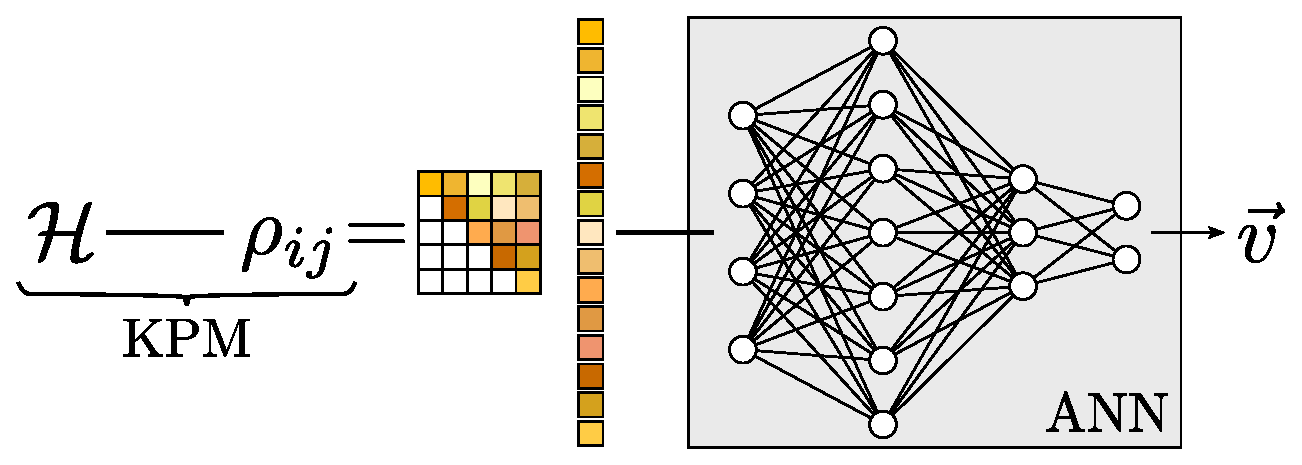
\includegraphics[width=\columnwidth]{ann/figures/fig2.pdf}
\vspace{-5pt}
\caption{
Sketch of the process to evaluate the topological character of a local region
of space. The density matrix corresponding to a certain area in space is
calculated using the KPM, after removing the redundant elements the matrix is
rearranged in a 1D array that is used as input for neural network that will
provide the corresponding topological invariant as output.
}
\label{fig_method}
\end{figure}
%~~~~~~~~~~~~~~~~~~~~~~~~~~~~~~~~~~~~~~~~~~~~~~~~~~~~~~~~~~~%



\subsection{Correlation functions with the Kernel Polynomial method}
\label{sec:KPM}
In this section we review how real space correlation functions can be
efficiently calculated using the Kernel polynomial method
(KPM).\cite{Weisse2006}
We will focus the discussion in the case of a normal electronic system,
since the case of a superconductor can be treated in an analogous way.
The main task that we have to perform is to obtain the density matrix, evaluated
in a restricted area of real space, of a certain (very large) Hamiltonian. In
terms of the eigenfunctions $|\Psi_k\rangle$ of the Hamiltonian $H$,
the elements of the density
matrix can be written as
\begin{equation}
\rho_{ij} = \int_{-\infty}^{E_F} \langle i | \Psi_k \rangle \langle \Psi_k | j\rangle\delta(E_k -\omega) d\omega
\label{dens}
\end{equation}
where $|i\rangle$ and $|j\rangle$ are the elements of the basis for the
Hamiltonian $H$ and $E_F$ is the Fermi energy.
The diagonal elements of the matrix, $\rho_{ii}$, are the integrated local
density of
states.
In the gapped state, the off-diagonal elements are expected to decay
exponentially with distance. So, when the Fermi energy $E_F$ lies in the gap,
the density matrix is properly described by restricting the calculation to a set
of neighboring sites.
Generically, calculating the previous matrix requires diagonalizing the full
Hamiltonian to obtain the occupied wavefunctions, a task that scales with
$\mathcal{O}(N^3)$, with $N$ the system size of the system.
The Kernel Polynomial Method allows the computation of $\rho_{ij}$, for a
restricted set of neighboring sites, with a computational cost that scales only
as $\mathcal{O}(N)$.

The KPM allows to compute the quantity
\begin{equation}
g_{ij}(\omega) = \sum_k \langle i | \Psi_k \rangle \langle \Psi_k | j\rangle\delta(E_k -\omega)
\end{equation}
which can easily be integrated to obtain the density matrix~\eqref{dens}. The
central idea is that $g_{ij}$ can be expressed in matrix form as
\begin{equation}
g_{ij}(\omega) =
\langle i | \delta (H-\omega) | j \rangle
\label{eq5}
\end{equation}

The KPM consists on expanding equation~\eqref{eq5} in terms of Chebyshev
polynomials $T_n(\omega)$. To do so, the Hamiltonian is first rescaled so that
all the eigenenergies lie in the interval $\mathcal{E}_k \in (-1,1)$. The
rescaled Hamiltonian is denoted as $\mathcal{H}$. The corresponding spectral
function is calculated as
\begin{equation}
g_{ij}({\omega}) = \frac{1}{\pi \sqrt{1-\omega^2}}
\left (\bar \mu_n + 2 \sum^N_{n=1} \tilde \mu_n T_n (\omega)
\right )
\label{KPM}
\end{equation}
The coefficients $\tilde \mu_n$ determine the expansion of a certain element
$g_{ij}$, and are calculated as

\begin{equation}
\tilde \mu_n = g^N_n \mu_n
\end{equation}
where $\mu_n$ are the coefficients calculated from the Hamiltonian
$\mathcal{H}$ and $g_n^N$ denotes the Jackson Kernel that improves the
convergence of the series\cite{Weisse2006,Jackson1912}

\begin{equation}
g_n^N =
\frac{(N-n-1)\cos \frac{\pi n}{N+1} + \sin \frac{\pi n}{N+1}
\cot \frac{\pi }{N+1}
}
{N+1}
\end{equation}

Given two sites $i$ and $j$, we define two vectors located in those sites
$v_i$ and $v_j$.
The coefficients $\mu_n$ would be calculated as a conventional functional
expansion

\begin{equation}
\mu_n = \langle v_i | \int_{-1}^{1}\delta (\mathcal{H}-\omega)T_n(\mathcal{H}) d \omega | v_j \rangle
\end{equation}
which in the diagonal basis reads
\begin{equation}
\mu_n = \int_{-1}^{1}\langle v_i | \Psi_k \rangle \delta (\mathcal{E}_k-\omega) \langle \Psi_k | v_j \rangle T_n(\omega) d \omega
\end{equation}
Performing the integration over $\omega$ we get
\begin{equation}
\mu_n = \langle v_i | \Psi_k \rangle T_n(\mathcal{E}_k)  \langle \Psi_k | v_j \rangle =
\langle v_i | T_n(\mathcal{H}) | v_j \rangle
\end{equation}
Therefore, the coefficients $\mu_n$ can be calculated as the overlap of two
vectors

\begin{equation}
\mu_n =
\braket{v_j}{\alpha_n}%\langle \alpha_0 | \alpha_n \rangle
\end{equation}
where $\alpha_n$ is calculated with
the recursion relations associated to the Chebyshev polynomials
\begin{equation}
\begin{aligned}
\ket{\alpha_0} = \ket{v_i}  \\  %|\alpha_0 \rangle = | v_i \rangle \\
|\alpha_1 \rangle = \mathcal{H} | \alpha_0 \rangle \\
|\alpha_{n+1} \rangle = 2\mathcal{H} | \alpha_n \rangle-
| \alpha_{n-1} \rangle
\end{aligned}
\end{equation}
This procedure thus involves matrix vector products to calculate the
coefficients. For a sparse matrix, as it is the case of a tight binding
Hamiltonian, the number of non-zero elements scales linearly with the system
size, so the computational cost of calculating the density matrix for a fixed
number of sites also scales linearly.
This method allows to compute $g_{ij}$ at every energy simultaneously, so
that $\rho_{ij}$ can be calculated by integration up to the Fermi energy.


For small systems, the density matrix can be calculated also by exact
diagonalization of the full Hamiltonian. In principle, that procedure
allows to calculate the
correlation function of relatively large one dimensional systems. However, for a
two dimensional system, the dimension of the matrix will be too large in
general. It is in that situation when the kernel polynomial method is specially
suitable.


\section{Topological invariants with supervised learning}
\label{sec:Topo}
We now describe the procedure to characterize the local topological character of
a system using ANN.
We choose as input the elements of the density matrix that involve one site and
its closest neighbors.
This procedure allows to naturally treat systems without translation
symmetry and with disorder, as the calculation of the density matrices is not more
computationally expensive in those situations using the previous procedure.
% Noel: This sentence was a bit weird for me
The process to calculate the density matrix was discussed in
Sec.~\ref{sec:KPM} but in order to use the density matrix as input for our ANN
some processing is required.
The density matrix is, in general, a complex Hermitian matrix, so we will
remove the redundant elements (namely the lower triangle) and arrange the
remaining elements in a 1D array, concatenating the real and imaginary parts.
Furthermore, we included the eigenvalues of the density matrix as part of the
input. Strictly, the inclusion of the eigenvalues is a redundant operation that
could be avoided by increasing the size and/or depth of the ANN, yet we found
that it helped the optimization of the model with a negligible computational
overhead.
The output of the ANN will be the topological invariant of the system.
The calculation of the corresponding output is done by constructing a
translational invariant Hamiltonian in which the corresponding topological
invariant is well defined and can be calculated in a standard way.
Finally, since we are using the ANN as a classifier, it is convenient to encode
the possible outputs as linearly independent vectors, $\vec{v}$, rather
than use a single scalar. The use of vectors allows the discrimination
between wrong answers and false positives.
This whole architecture is sketched in Fig. \ref{fig_method}.



In order to train of the ANN we generate a large number of realizations of a
family of Hamiltonians, exploring their parameter space. For a given choice of
parameters, we compute the topological invariant of the corresponding pristine
case and its local density matrix.
These procedure allows us to generate a set of inputs and outputs, which are
used to train the NN.
Once the ANN is trained, the model is ready to be evaluated with new data that
the network has never tried to test the accuracy of the network.
The last step is to create a new Hamiltonian with spatially dependent
parameters, and evaluate the ANN with the local density matrix corresponding to a
neighborhood of every lattice site.
In this way, we have a procedure to locally evaluate the topological
invariant of a systems lacking translational symmetry.




\subsection{One dimensional topological superconductor}
\label{sec:1d}
%~~~~~~~~~~~~~~~~~~~~~~~~~~ FIGURE ~~~~~~~~~~~~~~~~~~~~~~~~~%
\begin{figure}[t!]
\centering
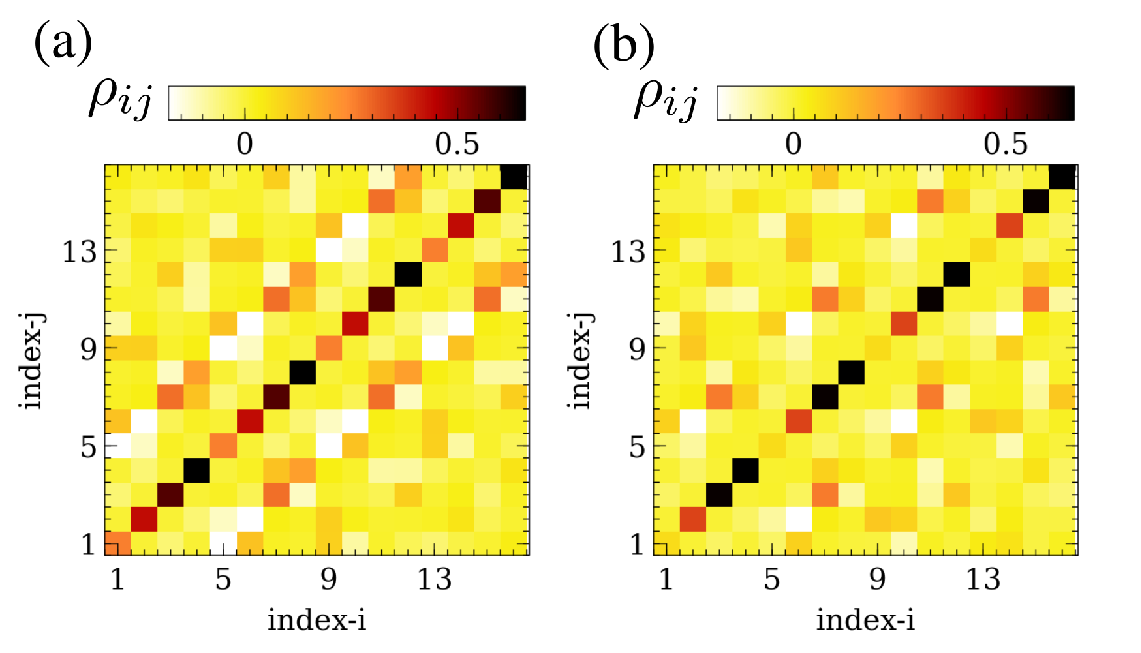
\includegraphics[width=0.5\textwidth]{ann/figures/fig3.pdf}
\vspace{-5pt}
\caption{
%Matrix
Image representation of the density matrix for two particular different states
for the superconducting 1D system, trivial (a) and topological (b). In terms of
the matrices shown, the task of the neural network can be understood as an image
recognition algorithm capable of distinguishing an input (a) from (b), for
different parameters of the Hamiltonian chosen randomly. The different indexes
in x and y axis run over spin and electron/hole sectors in the closest sites.
}
\label{fig3}
\end{figure}
%~~~~~~~~~~~~~~~~~~~~~~~~~~~~~~~~~~~~~~~~~~~~~~~~~~~~~~~~~~~%

In the following, we will consider a lattice model Hamiltonian for a one
dimensional electron gas that is able to host both trivial and topological
superconducting states. The corresponding topological invariant is a $Z_2$
number that can be calculated as a Berry phase.\cite{PhysRevB.88.075419}
Such effective one dimensional system, in particular the superconducting
topological phase, is realized in semiconducting nanowires deposited on top of a
s-wave
superconductor.\cite{PhysRevLett.105.077001,PhysRevLett.105.177002,mourik2012signatures,PhysRevB.84.144522,PhysRevLett.106.127001,lutchyn2017realizing,aguado2017majorana}
The model describes electrons in a 1D chain, in the presence of Zeeman
field, Rashba spin-orbit coupling, superconducting proximity effect
and a sublattice imbalance term.
Thus, the model has six different parameters: a spin-conserving hopping $t$,
chemical potential $\mu$, Rashba spin orbit $t_R$, external Zeeman field $B_z$,
on-site pairing term $\Delta$ and a trivial mass $m$.
Moreover, we also include the possibility of having finite Anderson disorder
$W_i$,
so that the full Hamiltonian reads

\begin{equation}
\begin{split}
  \mathcal{H} =&-t\sum_{\langle ij\rangle_\alpha}
                \crea{c}{i\alpha}\des{c}{j\alpha}
                 + i t_R\sum_{\langle ij\rangle_{\alpha\beta}}
      \hat{e}_z\cdot(\vec{\sigma}_{\alpha\beta}\times\vec{d}_{ij})
                                           \crea{c}{i\alpha}\des{c}{j\beta}\\
      &+B_z\sum_{i\alpha}\crea{c}{i\alpha}\sigma_z\des{c}{i\alpha}
  +\Delta \sum_i [c_{i\uparrow} c_{i\downarrow} + c^\dagger_{i\downarrow} c^\dagger_{i\uparrow}]\\
  &+ \mu\sum_{i,\alpha}\crea{c}{i\alpha}\des{c}{i\alpha}
  +m\sum_{i}\tau_i\crea{c}{i}\des{c}{i}
  +\sum_{i,\alpha} W_i \crea{c}{i\alpha}\des{c}{i\alpha}
  \label{hamil1d}
\end{split}
\end{equation}

The previous Hamiltonian can have topological and trivial phases.
In a nutshell, a topological phase may arise when the Zeeman term $B_z$ is such
that the chemical potential $\mu$ crosses only one of the spin channels, so that
a small pairing $\Delta$ and Rashba field $t_R$ gives rise to a spinless p-wave
superconductor.\cite{PhysRevLett.106.127001}
In the absence of both Zeeman and Rashba couplings, the induced superconducting
gap is trivial.


The Hamiltonian \eqref{hamil1d} is solved in the Nambu representation by defining
a spinor wavefunction as
$
%\begin{equation}
\Psi^\dagger =
\begin{pmatrix}
c^\dagger_{\uparrow}, &
c^\dagger_{\downarrow} ,&
c_{\downarrow}, &
-c_{\uparrow}
\end{pmatrix}
%\end{equation}
$
which gives rise to a Bogoliuvov-de-Gennes Hamiltonian
$\mathcal{H} = \frac{1}{2}\Psi^\dagger H \Psi$.
The matrix $H$ is used to calculate the correlation functions
$\langle c_{i,s} c_{j,s'} \rangle$
and
$\langle c^\dagger_{i,s} c_{j,s'} \rangle$,
as introduced in section~\ref{sec:KPM}, by integrating the different
$g_{ij}(\omega)$ from $\omega=-\infty$ up to $\omega=0$.
In Fig.~\ref{fig3} we show an example of two different input data from the
training dataset, for a topological (a) and a trivial (b) state computed for an
open chain with $N=400$ sites using the KPM.
It is evident that simple inspection is not enough to distinguish between the two
of them. 
%Interestingly, the lack of an analytic description for the
%topological invariant based solely in the local information makes the
%recognition of the different phases a non-trivial task, that our ANN is able to
%handle.

In order to generate the training dataset we considered different Hamiltonians
for a bipartite chain with 400 sites by varying the different values for the
off-plane Zeeman field $B_z$, Rashba $\lambda_R$, chemical potential $\mu$, 
superconducting pairing $\Delta$ and sublattice imbalance $m$.
In order to prove the robustness of our procedure, we also
switch on the Anderson on-site
disorder ($W\in (0.0,0.4t)$), with
a magnitude comparable to the other energy scales.
For the training dataset we generated 1000 different Hamiltonians with
parameters randomly chosen in the following ranges:
$t_R\in[-0.3t,0]$, $B_z\in[0.2t,0.8t]$, $\mu\in[t,2t]$, $\Delta\in[0.1t,0.3t]$,
$m\in[-0.2t,0.2t]$, 
yielding a five dimensional phase space. Using the generated Hamiltonians we
calculate the density matrix of the central atom in the nanowire, $\rho_{ij}$,
and its three closest neighbors.
Since the Hamiltonian in eq.~\eqref{hamil1d} only involves two Pauli matrices for
a linear chain, the Hamiltonian in real space can be chosen to be purely real,
so that its density matrix will be also real.
For each example the $Z_2$ topological invariant is calculated for the pristine
system ($W_i=0$)
defined by that particular set of parameters, which is used as expected
output. Since this topological invariant only has two possibilities, we encode
the $Z_2$ invariant as a two dimensional vector $v$, so that the topological
case corresponds to $v=(1,0)$ and the trivial case to $v=(0,1)$.
With this methodology a single element of the training dataset has a
152-dimensional input and a 2-dimensional output.
We took two hidden layers with 101 and 21 neurons.
After training, a validation set with 200 new samples is generated to test the
accuracy of the ANN yielding an accuracy of $\sim97\%$.
In order to gain some insight on the ANN capabilities, we run a simple test by
freezing all the parameters in the Hamiltonian~\eqref{hamil1d} but the chemical
potential and comparing the actual $Z_2$ with the output provided by the ANN.
In Fig~\ref{fig4}~(a) we see that even for unseen data the ANN is able to provide
the correct topological invariant.

Once the network is trained, it is ready to be used in the case of an inhomogeneus
system.
We now generate a one dimensional system following equation~\eqref{hamil1d} with
spatially varying couplings.
In particular, we modulate the chemical potential along the chain as shown in
Fig.~\ref{fig4}~(b). Such modulation is feasible by means of local gates in the
experimental realizations involving semiconducting
nanowires.\cite{Gul20168}
With such modulation, we observe the emergence of zero energy modes in the local
density of states~\ref{fig4}~(c), which are expected to be a signature of a
boundary between a trivial and topological phase.
The evaluation of the topological invariant on every atomic position of the
chain can be carried out by feeding the local density matrix to the trained
neural network.
Our network shows that the different regions of the space have different
topological invariants as shown in Fig.~\ref{fig4}~(d).
It is observed that the points of space where the topological invariant changes
in Fig.~\ref{fig4}~(d) correspond to the location of the zero energy Majorana
modes, as seen in Fig.~\ref{fig4}~(c), validating the performance of our neural network.


%~~~~~~~~~~~~~~~~~~~~~~~~~~ FIGURE ~~~~~~~~~~~~~~~~~~~~~~~~~%
\begin{figure}[t!]
\centering
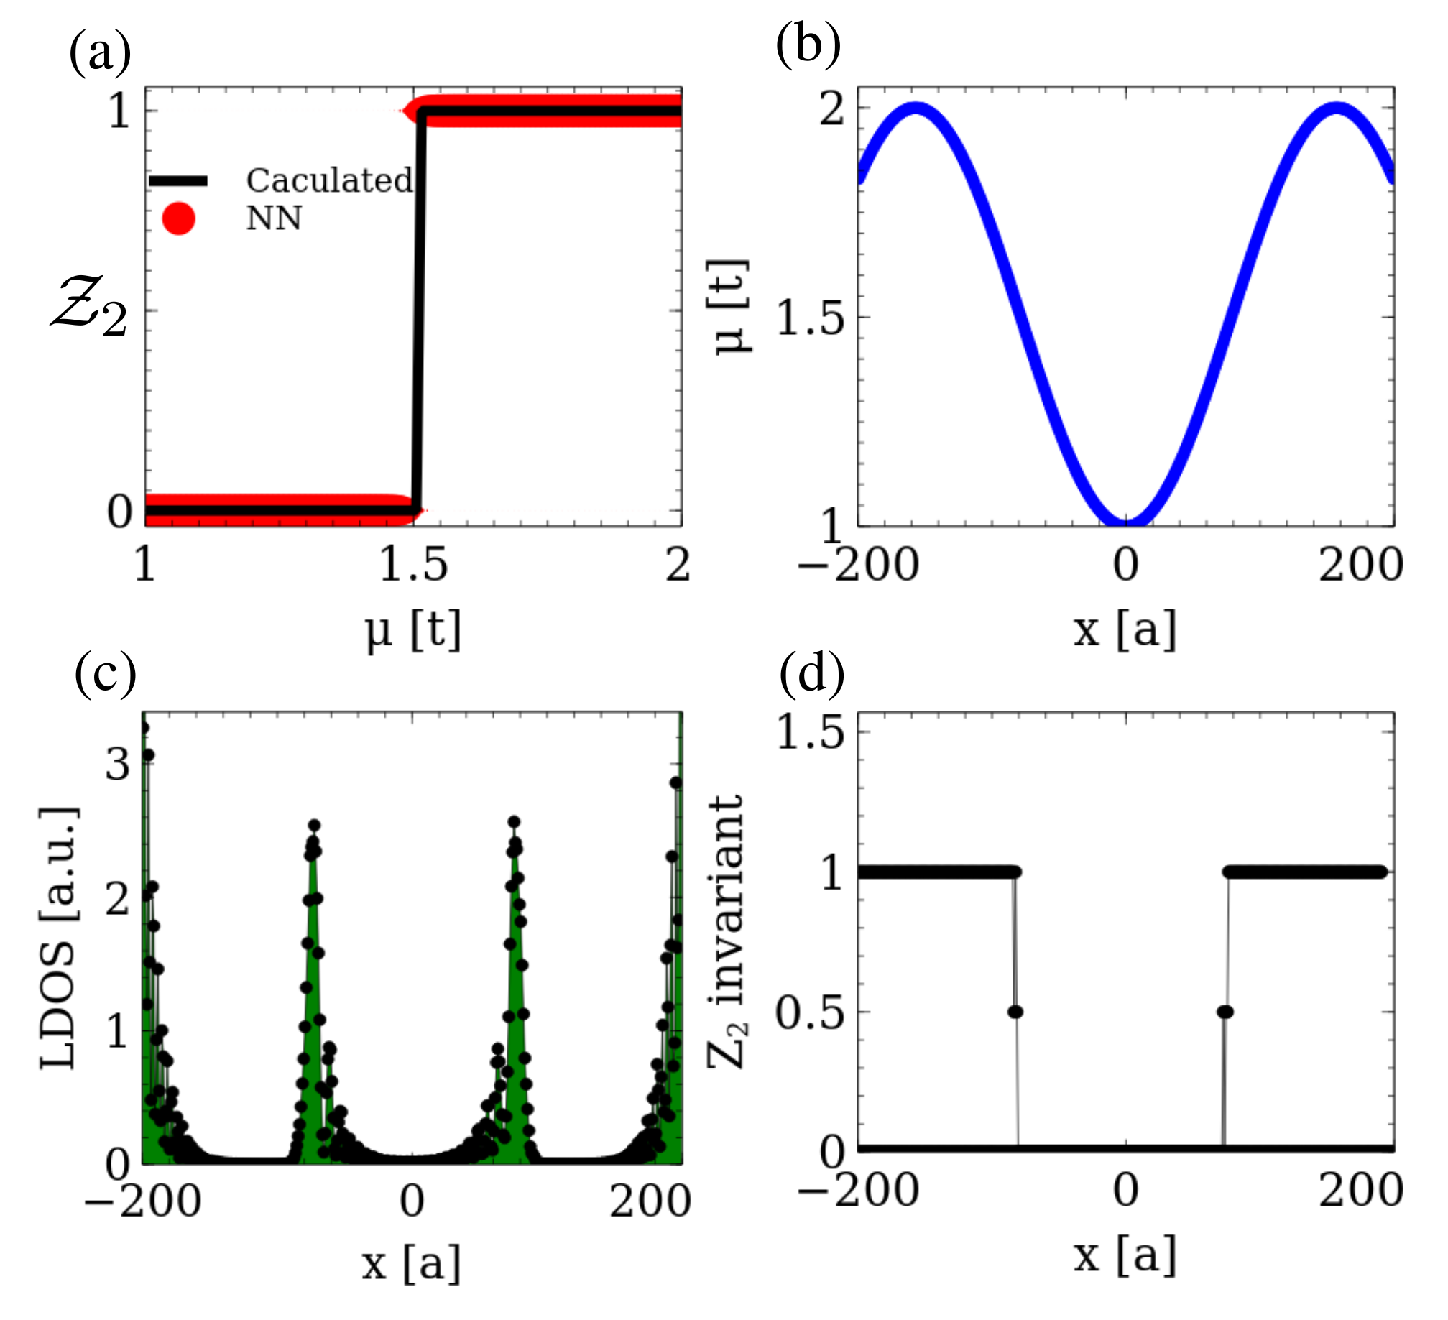
\includegraphics[width=0.45\textwidth]{ann/figures/fig4.pdf}
\vspace{-5pt}
\caption{
(a) Comparison of the topological invariant computed exactly with the one
predicted by the trained neural network in a pristine system,
showing that the ANN perfectly captures the phase transitions
in the homogeneus system. Afterwards, we
create a inhomogeneus system with modulated chemical potential as shown in
panel (b).
Such modulation creates trivial and topological zones, with Majorana modes
pinned at the transition points (c).
The neural network is then evaluated in every point of the space, yielding a
site-dependent topological invariant shown in (d). The topological
transitions shown in (d) mark the existence of zero Majorana modes obtained
in (c).
The parameters used are $\lambda_R=-0.3t$
%($Z_{ee,x}=Z_{ee,y}=0$,
$B_{z}=0.5t$, $m=0$, and $\Delta =0.1t$.
}
\label{fig4}
\end{figure}
%~~~~~~~~~~~~~~~~~~~~~~~~~~~~~~~~~~~~~~~~~~~~~~~~~~~~~~~~~~~%

The success of the neural network in describing the topological order of the
different phases implies that, locally, the density matrix carries
enough information to distinguish between the two cases. In particular, the
elements of $\rho_{ij}$ involving $\langle c_{i,s} c_{j,s'}\rangle$ encode
information about the induced superconducting order parameter, both in the $s$
and $p$-wave channels, which physically is expected to determine the topological
phase.
If, in comparison, only the diagonal part of the density matrix was used
as input for the neural network, it would not be possible to distinguish between
trivial and topological states.
This is easily understood taking into account that the diagonal part of
$\rho_{ij}$ accounts for the total occupation numbers and two topologically
inequivalent band-structures can have arbitrarily similar density of states.

\subsection{Two dimensional Chern insulator}
\label{sec:2d}
In this section we will use an analogous methodology to study a topological two
dimensional state. In particular, we consider a model Hamiltonian for
electrons moving in a honeycomb lattice with Rashba spin orbit coupling $t_R$,
off-plane exchange $B_z$, that is known to result in a two dimensional Quantum
Anomalous Hall state (QAH)\cite{Qiao2010}:
\begin{equation}
\begin{array}{c@{}l}
  H = -t\sum_{\langle ij\rangle_\alpha}\crea{c}{i\alpha}\des{c}{j\alpha}
    + i t_R\sum_{\langle ij\rangle_{\alpha\beta}}
    \hat{e}_z\cdot(\vec{\sigma}_{\alpha\beta}\times\vec{d}_{ij})
                                         \crea{c}{i\alpha}\des{c}{j\beta}\\
    +B_z\sum_{i\alpha}\crea{c}{i\alpha}\sigma_z\des{c}{i\alpha}
    % +\lambda_{m}  % for consistence with the other equation
    +m\sum_{i,\alpha}\tau_i\crea{c}{i\alpha}\des{c}{i\alpha}  \\
  +\sum_{i,\alpha} W_i \crea{c}{i\alpha}\des{c}{i\alpha}
  \end{array}
\label{hamil:2d}
\end{equation}
where $t_R$ is the Rashba coupling, $\vec{\sigma}$ are the spin Pauli matrices,
$B_z$ is the external Zeeman field and $\tau_i=\pm1$ is the sublattice operator.
The first term is the usual tight-binding hopping term, the second one describes
the Rashba interaction~\cite{Qiao2010,Min2006} and the third term is the
so-called exchange or Zeeman term which couples to the spin degree of freedom.
The fourth term is a trivial mass term that assigns an opposite on-site
energy for the atoms in each of the sublattices, that we introduce in order
to have a trivial insulator phase in the model.
Finally, the last term is an Anderson disorder term that we introduce
to prove the robustness of the procedure. For $m=0$, and $B_z\neq0$ and
$t_R\neq 0$, the model has a topological gap with a  with Chern number
$\mathcal{C}=\pm 2$. For $m\neq 0$ and $B_z=0$. the model has a trivial
($\mathcal{C}=0$) gap.

Each of these Hamiltonian terms can effectively describe different experimental
situations. The sublattice imbalance could arise for a graphene monolayer
deposited on boron nitride in a commensurate
fashion.\cite{wang2016gaps,PhysRevB.88.035448}
The Rashba and exchange fields naturally arise for a graphene monolayer
deposited over a ferromagnetic insulator, such as
YIG,\cite{tang2017approaching,PhysRevLett.114.016603}
EuO\cite{PhysRevB.95.075418} or
CrI$_3$.\cite{huang2017layer,zhang2017strong}
Furthermore, the non commensuration of graphene with the substrate creates Moire
patterns, resulting in an effective spatial modulation of the different
contributions.\cite{PhysRevB.90.075428,PhysRevB.96.085442,wang2016gaps}


%~~~~~~~~~~~~~~~~~~~~~~~~~~ FIGURE ~~~~~~~~~~~~~~~~~~~~~~~~~%
\begin{figure}[t!]
\centering
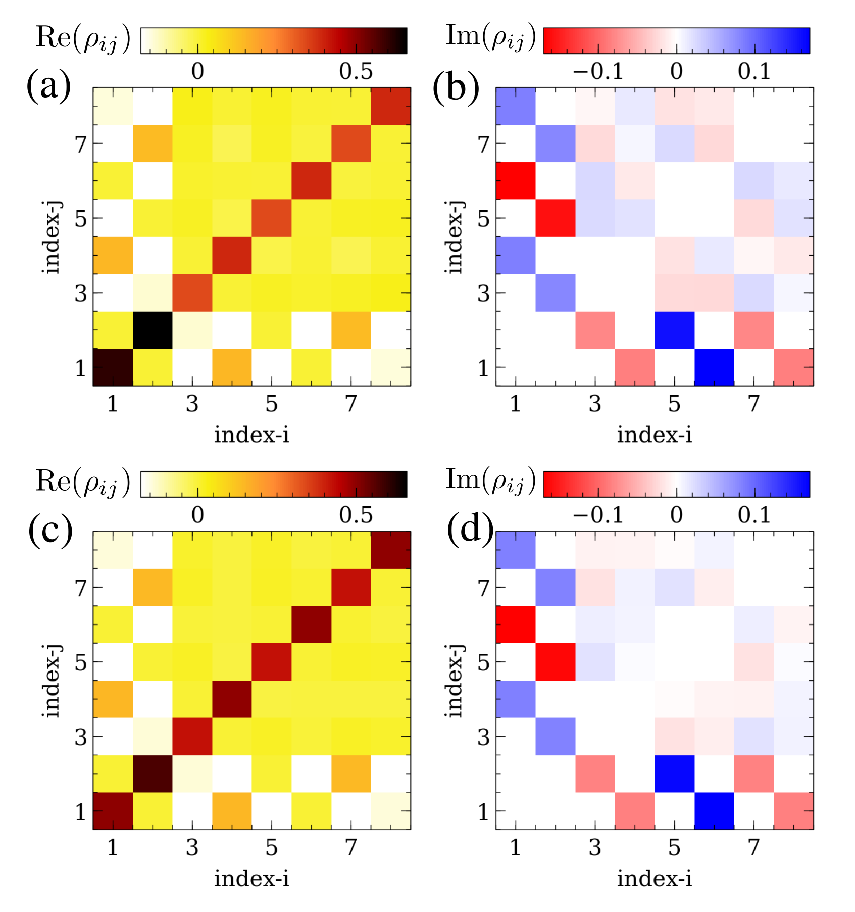
\includegraphics[width=0.5\textwidth]{ann/figures/fig5.pdf}
\caption{
Real and imaginary parts of the density matrix for a trivial $\mathcal{C}=0$ (a,b)
and a topological $\mathcal{C}=2$ (c,d) two dimensional system.
In this case, the neural network will implement an image recognition algorithm,
where the input are the two images representing the real and imaginary parts.
}
\label{fig5}
\end{figure}
%~~~~~~~~~~~~~~~~~~~~~~~~~~~~~~~~~~~~~~~~~~~~~~~~~~~~~~~~~~~%


It is worth mentioning two important differences with respect to the model
presented in Sec.~\ref{sec:1d}. On one hand, now the Hamiltonian involves the
three Pauli matrices, so in general it will be complex. This implies that the
calculated density matrices will also be complex, so that the neural network
will receive as input both the real and imaginary components.
On the other hand, since we are dealing now with a two dimensional system, a
finite island will have $L^2$ sites, with $L$ the typical size of the island.
In particular, the calculation of a the density matrix with the wavefunctions of
an island with side $L\approx 300$ would require the diagonalization of matrix
of dimension $L^2\approx 90000$, whose computational complexity is $L^6$. It is
in this situation where the KPM will be specially useful, as it allows us to
calculate the density matrix with a computational complexity of the number of
sites, $L^2$.


%~~~~~~~~~~~~~~~~~~~~~~~~~~ FIGURE ~~~~~~~~~~~~~~~~~~~~~~~~~%
\begin{figure}[t!]
\centering
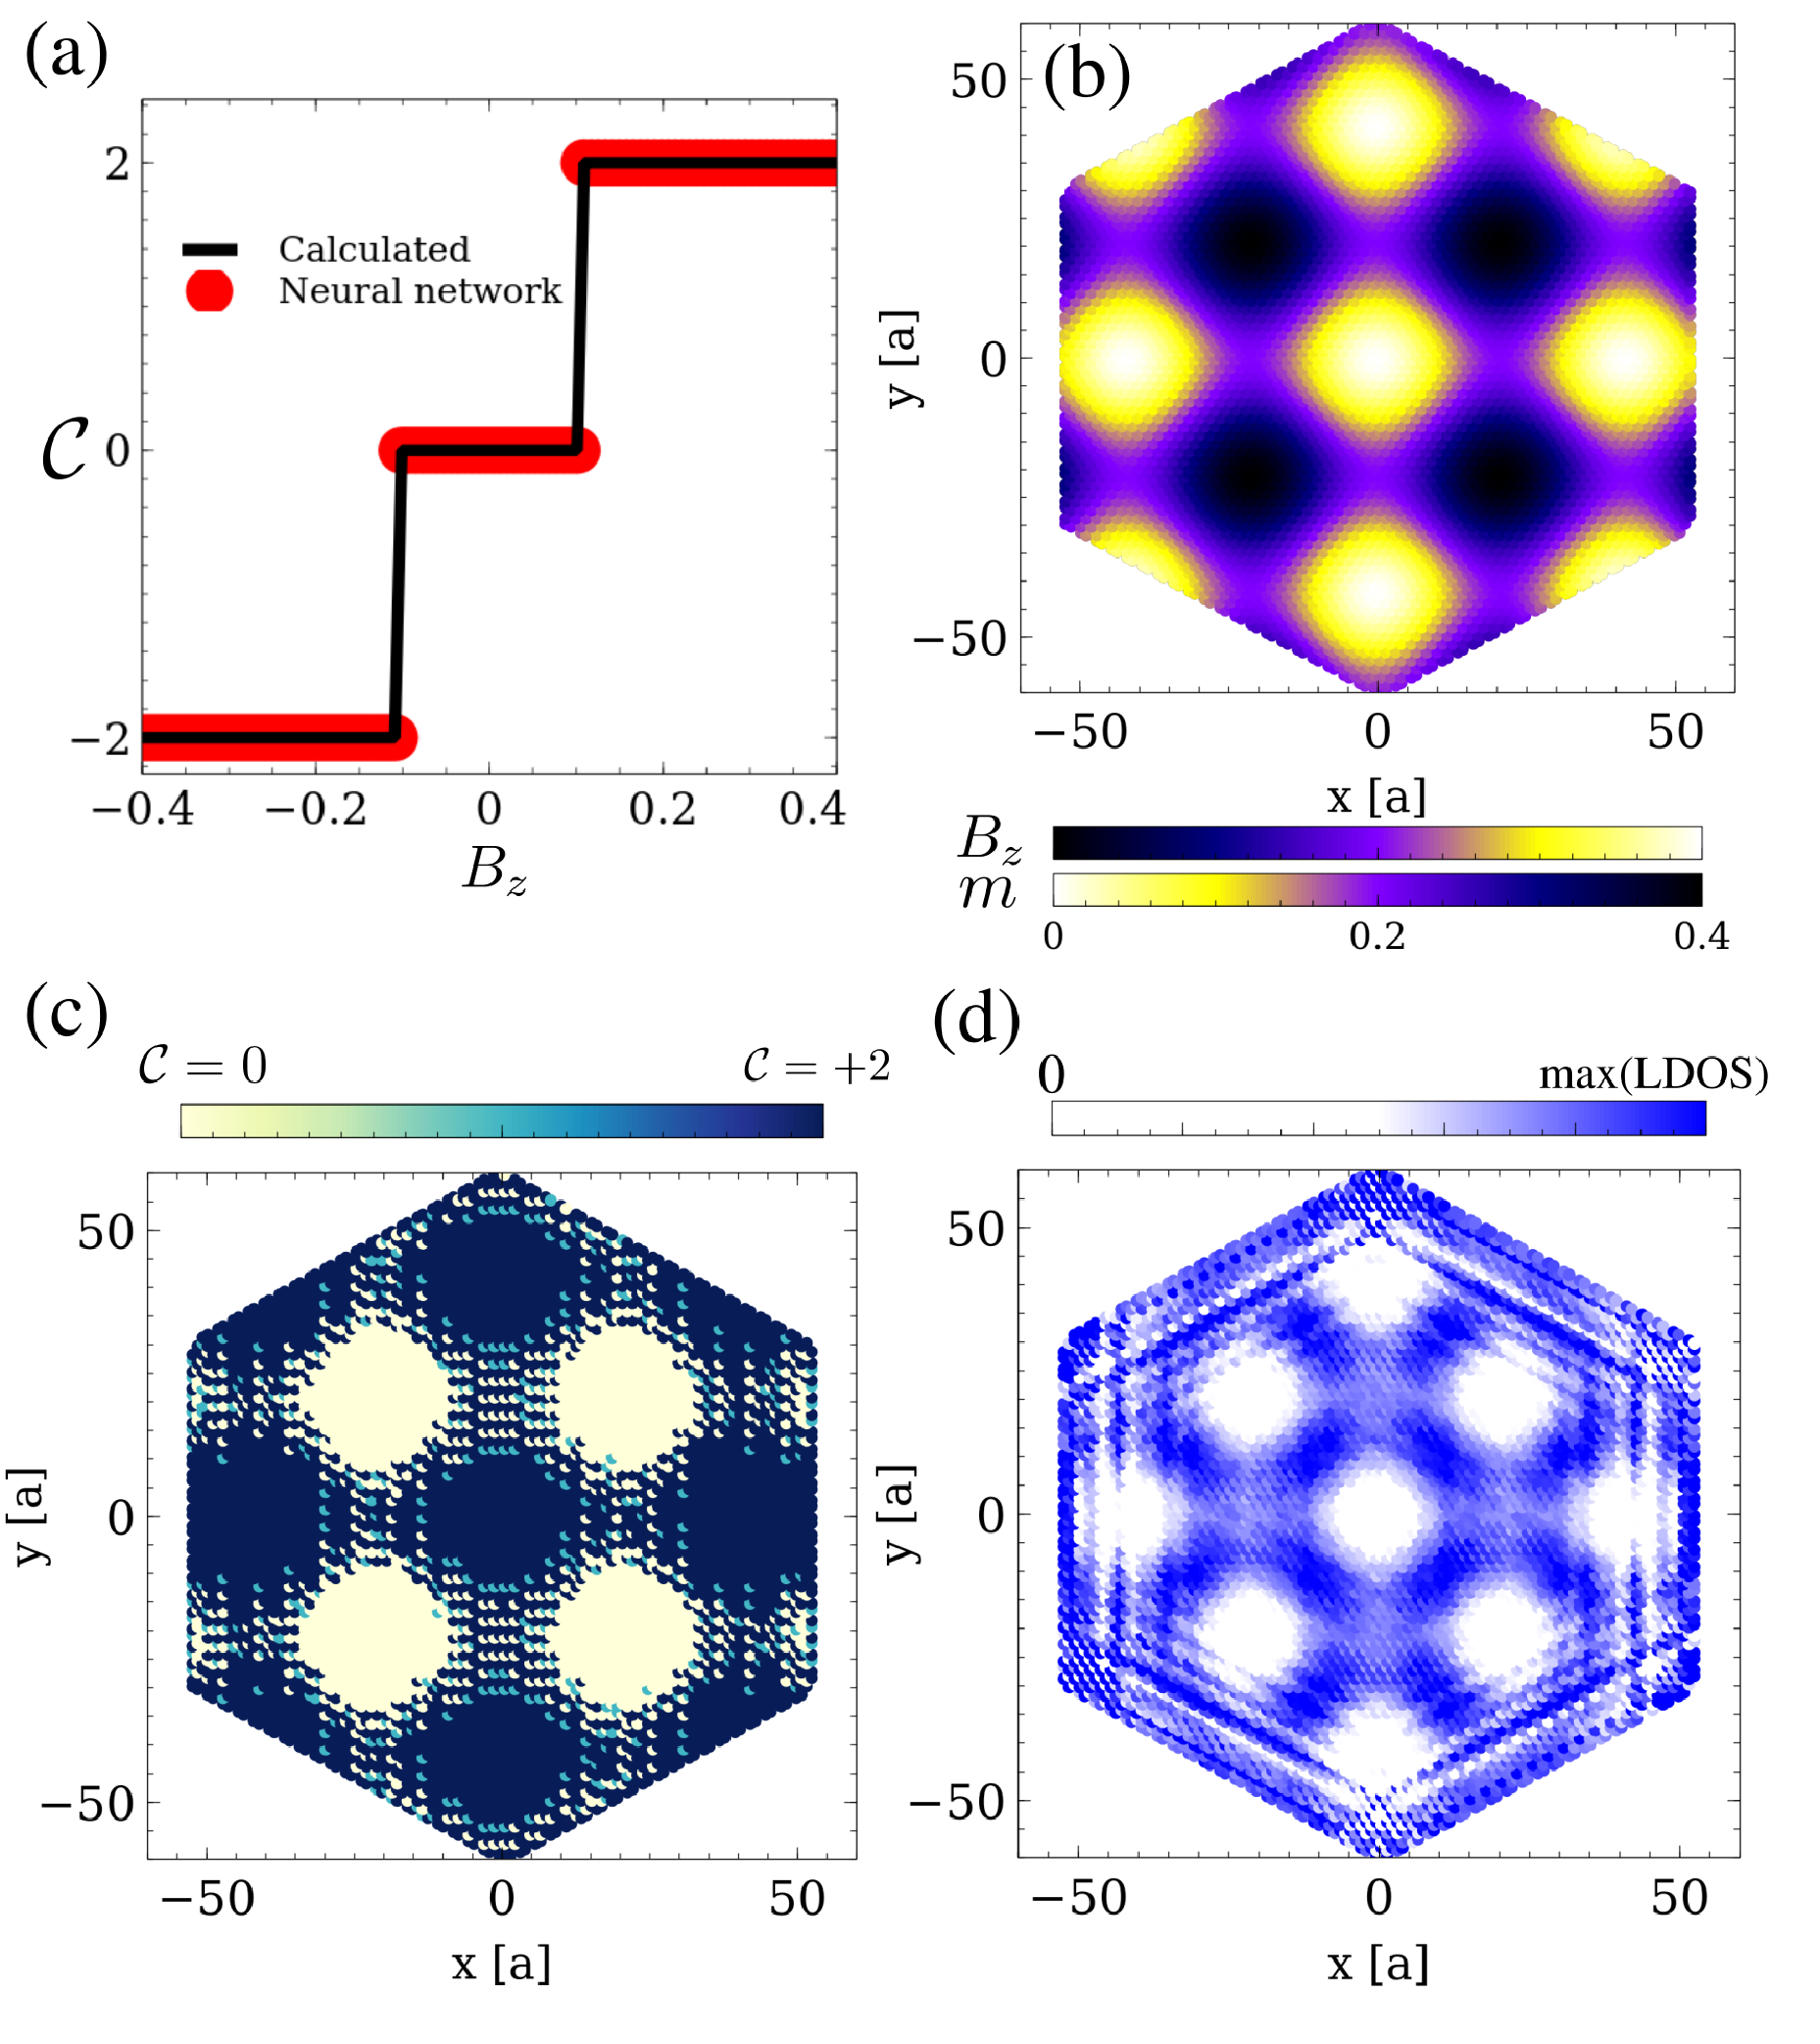
\includegraphics[width=0.5\textwidth]{ann/figures/fig6.pdf}
\caption{
(a) Comparison between the exact Chern number (black) and the prediction of the
trained neural network (red) using as input the local density matrix. Once the
accuracy of the network has been checked, we created a big graphene island with
modulated mass and exchange term as shown in (b). The neural network is used
to evaluate the topological invariant in each atom, yielding the result shown
in (c). The boundary between different topological phases is expected to give
rise to in-gap states, which is confirmed by calculating the in-gap spectral
function as shown in (d).
}
\label{DOS_fig}
\label{fig6}
\end{figure}
%~~~~~~~~~~~~~~~~~~~~~~~~~~~~~~~~~~~~~~~~~~~~~~~~~~~~~~~~~~~%

We now move to apply our methodology to the system defined by
eq.~\eqref{hamil:2d}.
First, to train the neural network, we generate different spatially uniform
Hamiltonians by choosing randomly each of the coupling parameters. The Zeeman
and Rashba were randomly generated in the interval $t_R\in[-0.4t,0.4t]$ and the mass
between $m\in[0,0.4t]$. Again, random Anderson-like disorder comparable to the other
interactions are introduced all across the system $W_i\in [0.0,0.4t]$.
The training dataset consisted in 564 samples. 
% and the testing dataset had 586 samples.
For every set of parameters, we built the Hamiltonian as in eq.~\eqref{hamil:2d}
and calculated the local density matrix for the central atom and its three first
neighbors which are used as input of the network, in this case a 128-dimensional
array.
Again we chose having two hidden layers with 101 and 21 neurons.
It is worth considering again the challenging task of distinguishing
between different inputs as those shown in Fig.~\ref{fig5}, which
highlights that the classification of topological and trivial phases based only
in local properties is far from being a trivial task.

The output for each input was obtained by calculating the Chern number of the
ground state of the system integrating the Berry curvature in the Brillouin zone
of a translational invariant ($W_i=0$) Hamiltonian with the same parameters.
Once the network was trained, we tested its  accuracy on a validation
dataset with 586 samples randomly generated,  showing an accuracy of $\sim92\%$.
The comparison of the result predicted by the network and the one calculated
exactly in  a system with translational invariance is shown in
Fig.~\ref{fig6}~(a) for the different topological phases.

After the training, we generated a graphene nano-island with 7400 atoms. In this
island, we choose a spatially modulated exchange field of the form
$B_z(x,y) = 0.1t[\cos(0.15 x)+\cos(0.15 y)+2]$, a modulated mass term of the form
$m(x,y) = 0.1t[\sin(0.15 x)+\sin(0.15 y)+2]$ (shown in Fig.~\ref{fig6}~(b)), and a
constant Rashba coupling $\lambda_R = 0.2$.
The previous modulations are expected to create neighboring trivial and
topological areas depending on which is the dominant contribution, mass or
exchange and Rashba couplings.
With such a Hamiltonian, we calculated the local density matrix using the Kernel
polynomial method, that was used as input of the neural network.
The result of the evaluation of the neural network across the sample is shown in
Fig.~\ref{fig6}~(c). % Note that the transition regions are somewhat troublesome for the ANN. This is due to the fact that these algorithms provide a smooth output, so it would require much more training to sharpen the transitions.
It can be seen that different regions with different Chern number appear according
to the spatial modulation of the Hamiltonian parameters.
The significance of the different regions becomes clear once the in-gap density
of states is calculated in Fig.~\ref{fig6}~(d). This shows both in-gap modes
precisely at the boundary between different regions, as expected form the
bulk-boundary correspondence,  as well as edge states all around the sample.

This result  highlights that the artificial neural network faithfully distinguishes
between the different phases based solely in local information, providing an
useful method to calculate the topological invariant in systems without
translational symmetry.



%%%%%%%%%%%%%%%%%%%%%%%%%%%%%%%%%%%%%%%%%%%%%%%%%%%%%%%%%%%%%%%%%%%%%%%%%%%%%%%%
\section{Conclusions}
\label{sec:Conc}
We have shown that an artificial neural network is capable of predicting the
topological nature of different model Hamiltonians using as an input a local
sector of the density matrix, {\em i.e.}, evaluating solely \emph{local properties}.
Our procedure consisted on training an artificial neural network using as
input the subspace of the density matrix corresponding to a local area of the
sample, and as output the topological invariant that an analogous (pristine and
translational invariant) Hamiltonian with the same effective parameters would
have.

We applied this procedure to two well known models,  a  1D
topological superconductor and 2D topological insulator. In both
cases we considered finite systems with a space dependent Hamiltonian that
create regions with both topological and trivial character.
By evaluating the network with local quantities for each Hamiltonian we showed
that the different topological domains are accurately identified by the network,
even when the inhomogeneus systems have Anderson-like disorder, proving that
this methodology can be applied for disordered systems.

It is worth remarking that the training procedure is carried out for a specific
model, and tested in that same model for different parameters, including local
modulations in space.
An open question is whether this methodology can be extended to cases with the
same topological classes but different geometries.
%Joaquin: not sure of what this means. Examples?
%Noel: This means for instance that we are not sure if it should work or not in another QASH that is realized in any other material that is not a honeycomb lattice
Finally, it is interesting to note that an analogous methodology could be
applied  
to interacting systems, so that similar procedures could be exploited
to identify
quantum spin liquid states in two dimensional spin systems.


%%~~~~~~~~ Chapter ~~~~~~~~
%\chapter{Graphene monolayer}
We consider a tight-binding model in the Slater-Koster (SK) approximation with 4 orbitals for the $C$ atom ($s$,$p_x$,$p_y$,$p_z$) and 1 orbital ($s$) for the $H$ atom. The SK parameters used are:
\begin{equation}
  \begin{array}{l|cccc}
        & V_{ss\sigma} & V_{sp\sigma} & V_{pp\sigma} & V_{pp\pi} \\ \hline
    C-C & -7.76 & 8.16 & 7.48 & -2.7 \\
    C-H & -6.84 & 7.81 & \text{--} & \text{--}
  \end{array}\qquad\qquad
  \begin{array}{c|cccc}
    \text{On-site} & s & p_x & p_y & p_z \\ \hline
    C & -8.8 & 0.0 & 0.0 & 0.0 \\
    H & -2.5 &     &     &
  \end{array}
\label{SK_params}
\end{equation}

These parmeters are in line with those found in the literature\cite{Gosalbez-Martinez2011,Konschuh2010} and can be obtained by fitting of DFT bands (done with quantum-espresso). It is important to notice that the exact values for these parameters is not relevant since small deformation of them just result in small deformations of the band structure. The symmetries of graphene and its orbitals ensure that the components of the eigenstates are the correct ones since the $p_z$ is decoupled from all the other orbitals.

With these parameters we consider an armchair hexagonal nanoisland ($\sim10^4-10^5$ $C$ atoms). Such a system is 0-dimensional, hence, no band structure can be defined but rather just the spectrum. Nevertheless, in the limit of an infinite island, the physical properties of graphene should be recovered.
We can get an idea of how far from real graphene we are by considering the confinement gap. Graphene is famously known for not having a gap in the band structure. Graphene nanoislands do have a gap due to its finite size, but the larger the island, the smaller the gap until in the limit of an infinite island (graphene) the gap shall disappear. The dependence of the gap and the size of the island can be estimated as a free particle in a box of size $L$, roughly $\Delta\sim\frac{1}{L^2}$. Performing the actual calculation we can obtain see the dependence of the gap with the size of the island (see Fig.~\ref{confinement}) and estimate the necessary dimensions for our calculations.

%~~~~~~~~~~~~~~~~~~~~~~~~~~ FIGURE ~~~~~~~~~~~~~~~~~~~~~~~~~%
\begin{figure}[h!]
  \centering
  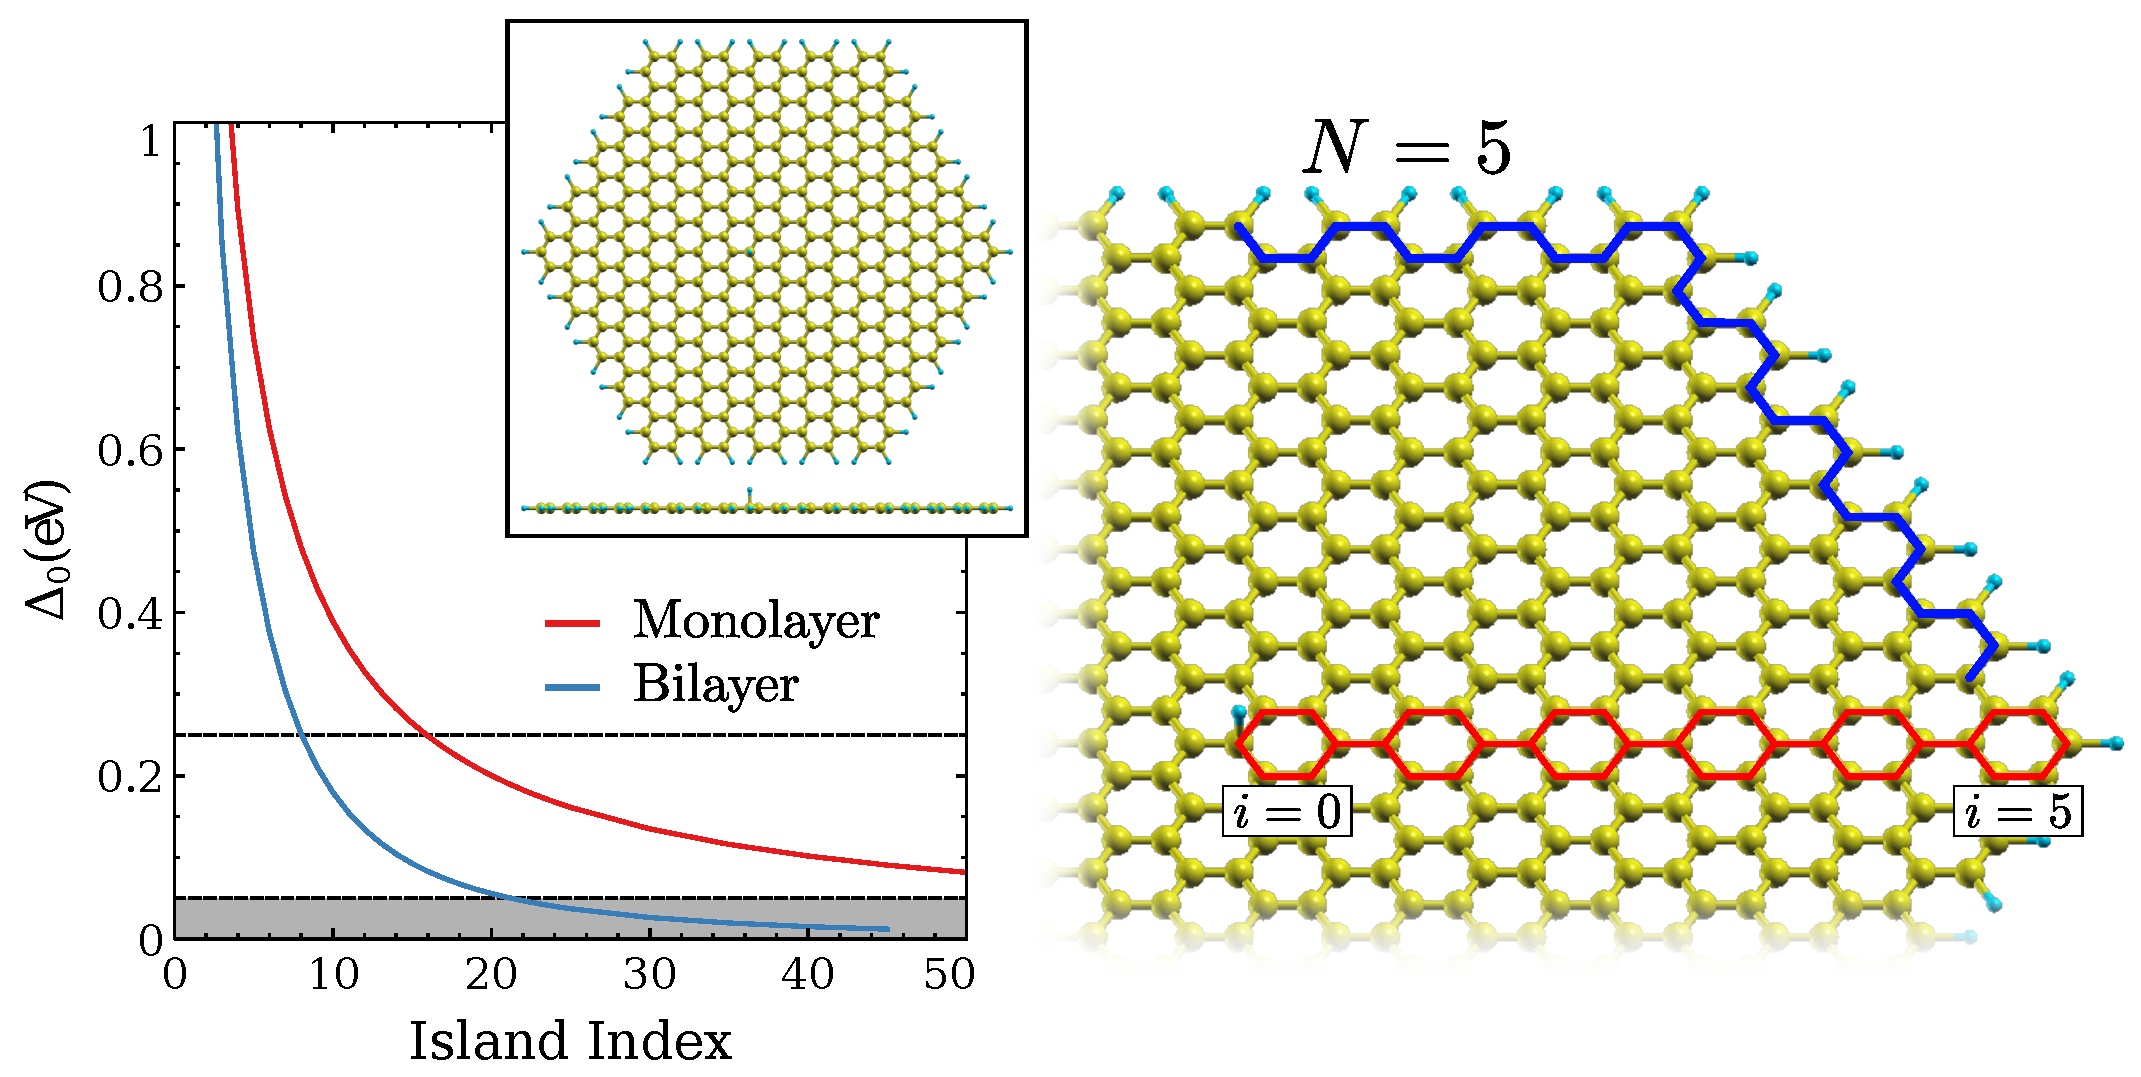
\includegraphics[width=0.9\textwidth]{defects/fig/cell.pdf}
  \vspace{-5pt}
\caption{Confinement gap for a monolayer and a bilayer of graphene. The island index labels the size of the island by the number of ``benzene blocks'' along the diagonal as shown in red in the right panel. The dashed line at $0.25eV$ corresponds to the largest gap opened bia electric gating in graphene bilayer\cite{Zhang2009}. We will consider the islands big enough to be considered as graphene when their confinement gap lies in the shadowed region.}
\label{confinement}
\end{figure}
% \FloatBarrier
%~~~~~~~~~~~~~~~~~~~~~~~~~~~~~~~~~~~~~~~~~~~~~~~~~~~~~~~~~~~%

When 4 orbitals are considered, the breaking of the $C_3$ symmetry at the edges (ie, the $C$ atoms in the edges are missing 1 neighbor) results in near-zero energy states due to the unmet $\sigma$ bonds, combination of $s$, $p_x$ and $p_y$. In order to get rid of these artificious states we consider the island edges to be pasivated by Hydrogen atoms as shown in Fig.~\ref{confinement}. This way the dangling bonds hybridize and get lifted/drowned to the $\sigma$ manifolds.
Although physically founded, the inclusion of $H$ pasivating atoms is somehow a technical construct to remove the dangling bonds from the low energy spectrum, hence, the strength of the $C-H$ bonds is not relevant and it should suffice to shift the $\sigma$ states far away from the low energy part of the spectrum.

% Such parameters yield the following band structure for graphene
\section{H adatom on graphene monolayer}
When a Hydrogen atom is placed on top of one of the $C$ atoms of graphene, the $s$ orbital of the Hydrogen hybridizes with both the $s$ and the $p_z$ orbitals of the Carbon. All the other hoppings are strictly zero due to the symmetry and disposition of the orbitals.

The general understanding is that a $H$ adatom on graphene can be understood as a vacancy in the $p_z$ subspace. The reason for this is that the $s$ orbital of the $H$ hybridizes with the $s$ and $p_z$ orbitals of the $C$ atom (all other hoppings vanish because of symmetry). In the scenario of a vacancy in the $p_z$ manifold, the system is exactly a bipartite lattice, and following (one of) the Lieb's theorems, the imbalance in the number of atoms in one of the sublattices results in zero energy states.

The Lieb's Theorem holds for bipartite lattices at half filling, which is indeed the case of graphene when only $p_z$ orbitals are considered. The inclusion of the other $p$ orbitals does not break the bipartite nature of the lattice since their manifold is disconnected from that of the $p_z$ orbitals, \emph{and their on-site energy is the same}.
The $s$ orbitals are also disconnected from the $p_z$ manifold but their on-site energy is different from zero (see \ref{SK_params}). This fact breaks the bipartite character of the lattice, nevertheless, the $s$ manifold is far in energy and its hybridization with the $p_{x/y}$ orbitals is strong so the bonding-antibonding states are also far in energy.

It is instructive to compare the spectrum of a big armchair island (22686 $C$ atoms) considering 4 orbitals and a $H$ adatom and the same island with only $p_z$ orbitals and a vacancy.

%~~~~~~~~~~~~~~~~~~~~~~~~~~ FIGURE ~~~~~~~~~~~~~~~~~~~~~~~~~%
\begin{figure}[h!]
  \centering
  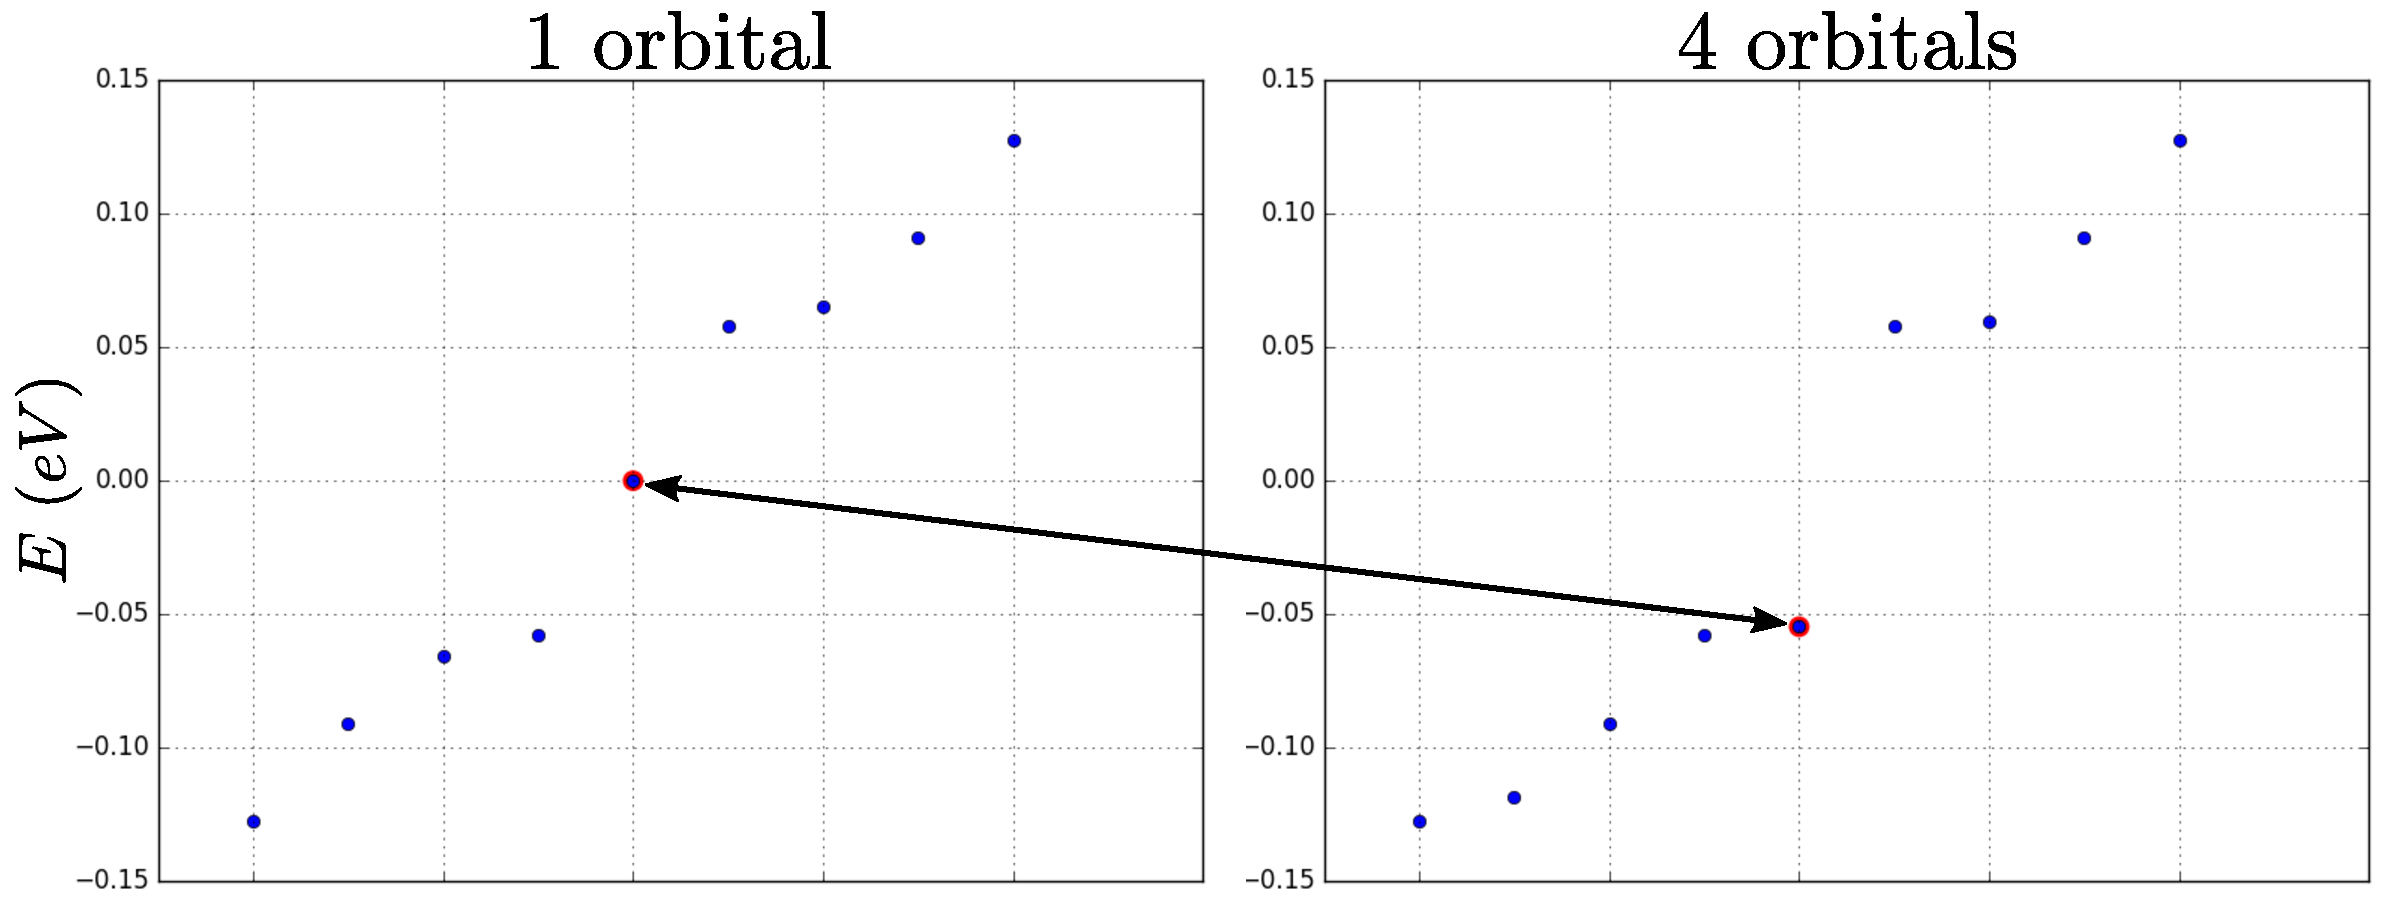
\includegraphics[width=0.8\textwidth]{defects/fig/spectrum.pdf}
  \vspace{-5pt}
\caption{Low energy spectrum of an armchair island. Left panel shows the spectrum when only the $p_z$ orbitals are considered. Right panel shows the spectrum considering all 4 orbitals $s$, $p_x$, $p_y$, $p_z$}
\label{spectrum}
\end{figure}
\FloatBarrier
%~~~~~~~~~~~~~~~~~~~~~~~~~~~~~~~~~~~~~~~~~~~~~~~~~~~~~~~~~~~%

Notice in figure~\ref{spectrum} that the in-gap state, marked in red, does not appear at $E=0$ as this system is no longer suitable for the Lieb's theorem. The exact energy at which the in-gap state appear depends on the hopping parameters between the $H$ and the $C$ atoms, mainly on the $V_{sp\sigma}$ parameter.

The parameters in \ref{SK_params} were calculated for $H$ pasivating the edges of graphene nanoribbons where the main hybridization occurs with the $\sigma$ orbitals of graphene. There is no good reason why these hoppings parameters should hold for an adatom, so we can consider the hopping parameters, $V_{ss\sigma}$ and $V_{sp\sigma}$, between the chemisorbed Hydrogen and graphene as somehow free parameters that we can tune.

The position of the in-gap state as a function of both parameters is shown in fig~\ref{ingap}. Notice the strong dependence with the $V_sp\sigma$ parameter.
%~~~~~~~~~~~~~~~~~~~~~~~~~~ FIGURE ~~~~~~~~~~~~~~~~~~~~~~~~~%
\begin{figure}[h!]
  \centering
  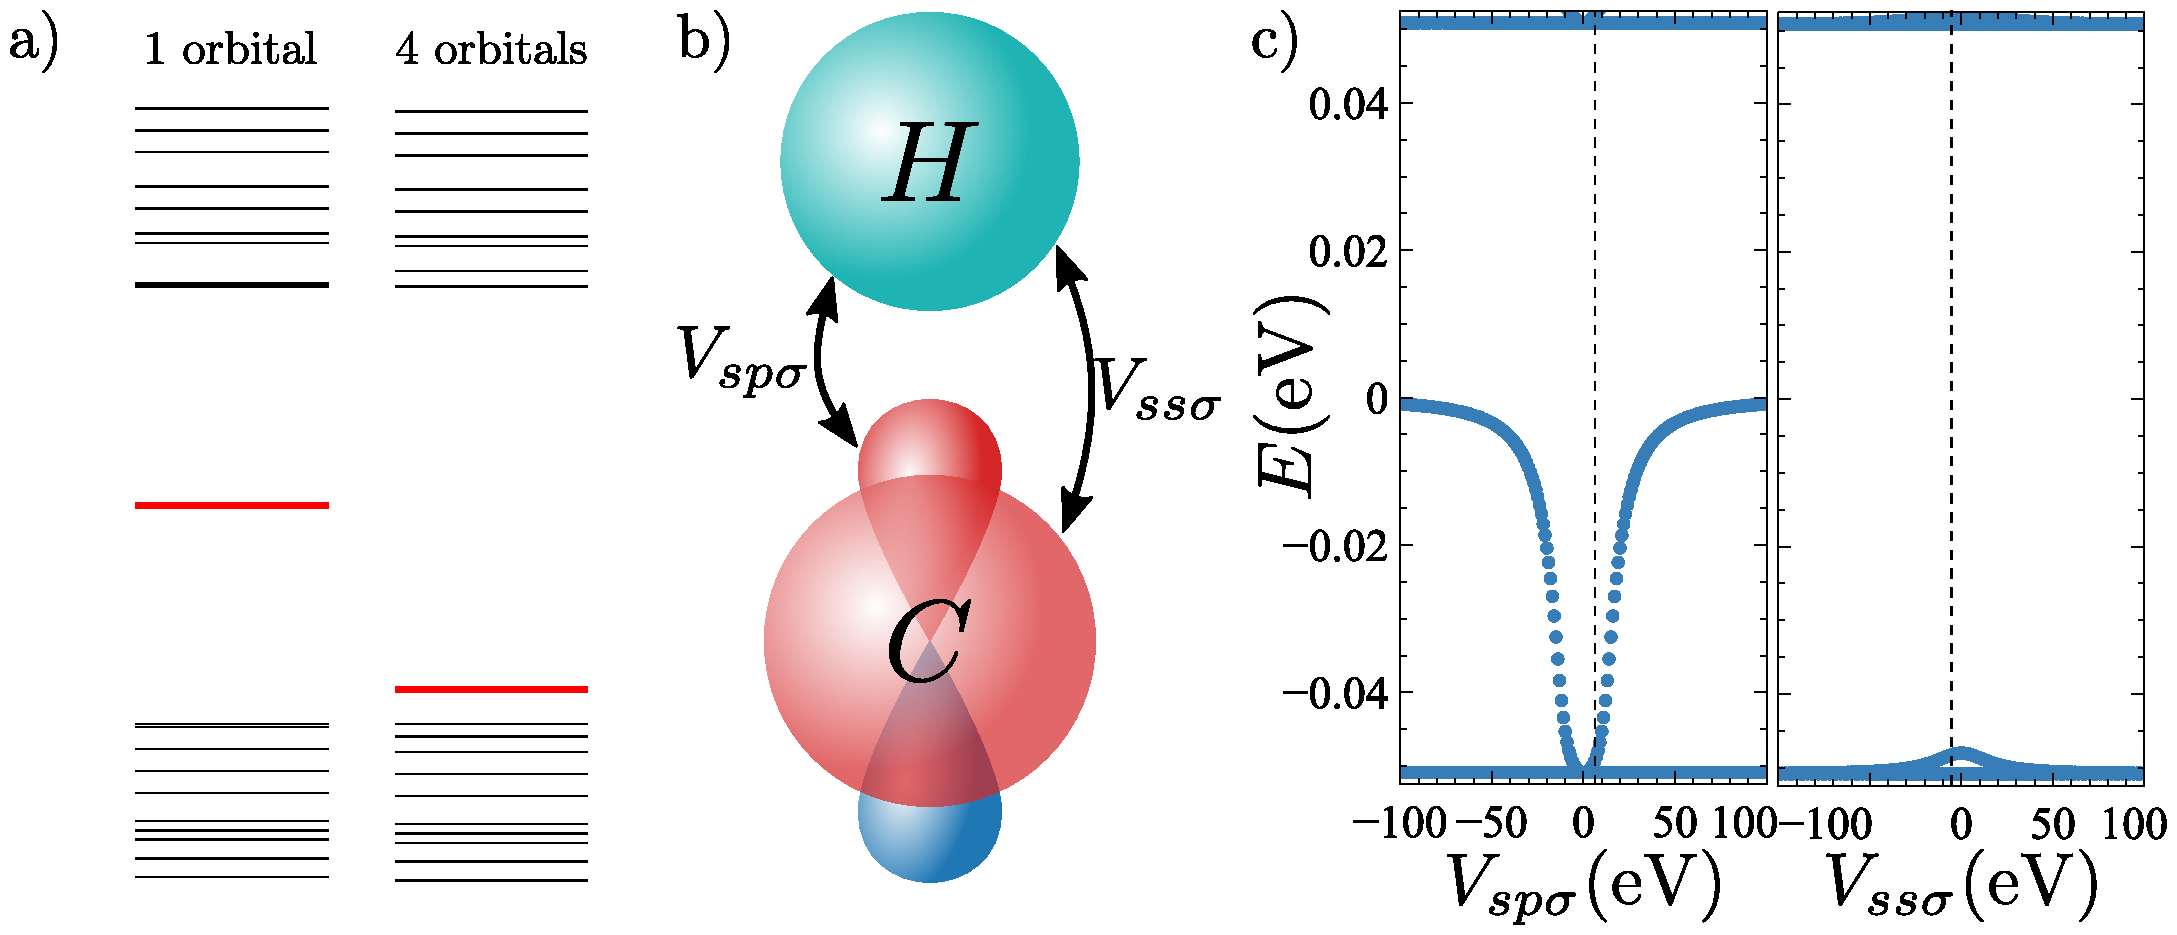
\includegraphics[width=0.8\textwidth]{defects/fig/Vsss_Vsps.pdf}
  \vspace{-5pt}
\caption{Position of the in-gap state of an adatom on a graphene nanoisland as a function of the hopping parmeters $V_{sp\sigma}$ and $V_{ss\sigma}$. In the plot the whole range to $\pm\infty$ is explored although the relevant part is only around 0, namely [-20,20].}
\label{ingap}
\end{figure}
\FloatBarrier
%~~~~~~~~~~~~~~~~~~~~~~~~~~~~~~~~~~~~~~~~~~~~~~~~~~~~~~~~~~~%
It is clear that in order to recover the 1 orbital intuition (in-gap state at $E=0$), we require the limit for $V_{sp\sigma}\to\infty$. The experimental value for these parameters is difficult to infer, so we will consider a wide range of value and explore the resulting physics.

We start by plotting the position of the in-gap state and the hyperfine coupling  as a function of the two parameters


%~~~~~~~~~~~~~~~~~~~~~~~~~~ FIGURE ~~~~~~~~~~~~~~~~~~~~~~~~~%
\begin{figure}[h!]
  \centering
  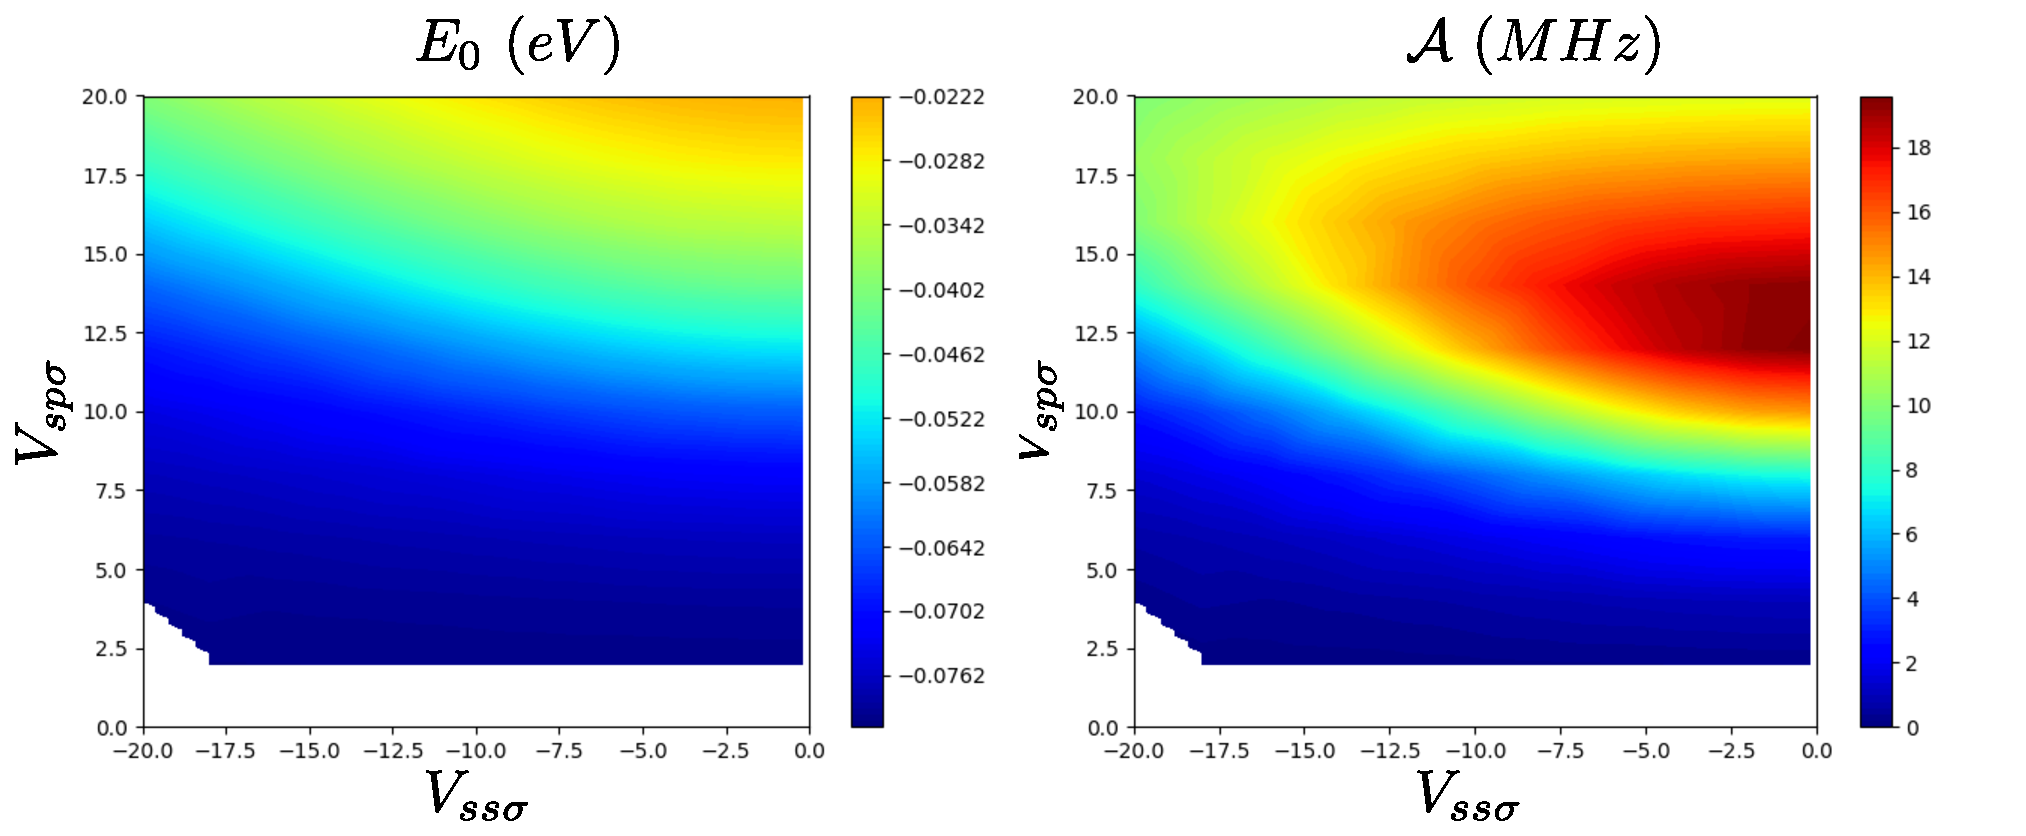
\includegraphics[width=0.9\textwidth]{defects/fig/parameter_space_mono.pdf}
  \vspace{-5pt}
\caption{Parameter space for the energy of the in-gap state and the hyperfine coupling for a graphene nanoisland.}
\label{SK2d}
\end{figure}
\FloatBarrier
%~~~~~~~~~~~~~~~~~~~~~~~~~~~~~~~~~~~~~~~~~~~~~~~~~~~~~~~~~~~%







\section{Graphene bilayer}
Graphene bilayer can be described in a analogously. The interlayer hopping is estimated by scaling down the parameters \eqref{SK_params} by a factor, $\xi$, such that the $p_z-p_z$ interlayer hopping takes a value\cite{KatsnelsonBook} of $\xi t_{p_z-p_z}\simeq 0.4eV$.
% Fig~\ref{hoppings} shows all the possible hoppings between two C atoms in different layers. It is important to notice that in the case of graphene bilayer, the $p_z$ manifold is no longer decoupled from the rest of the orbitals as in the case of graphene.
% %~~~~~~~~~~~~~~~~~~~~~~~~~~ FIGURE ~~~~~~~~~~~~~~~~~~~~~~~~~%
% \begin{figure}[h!]
% \centering
%   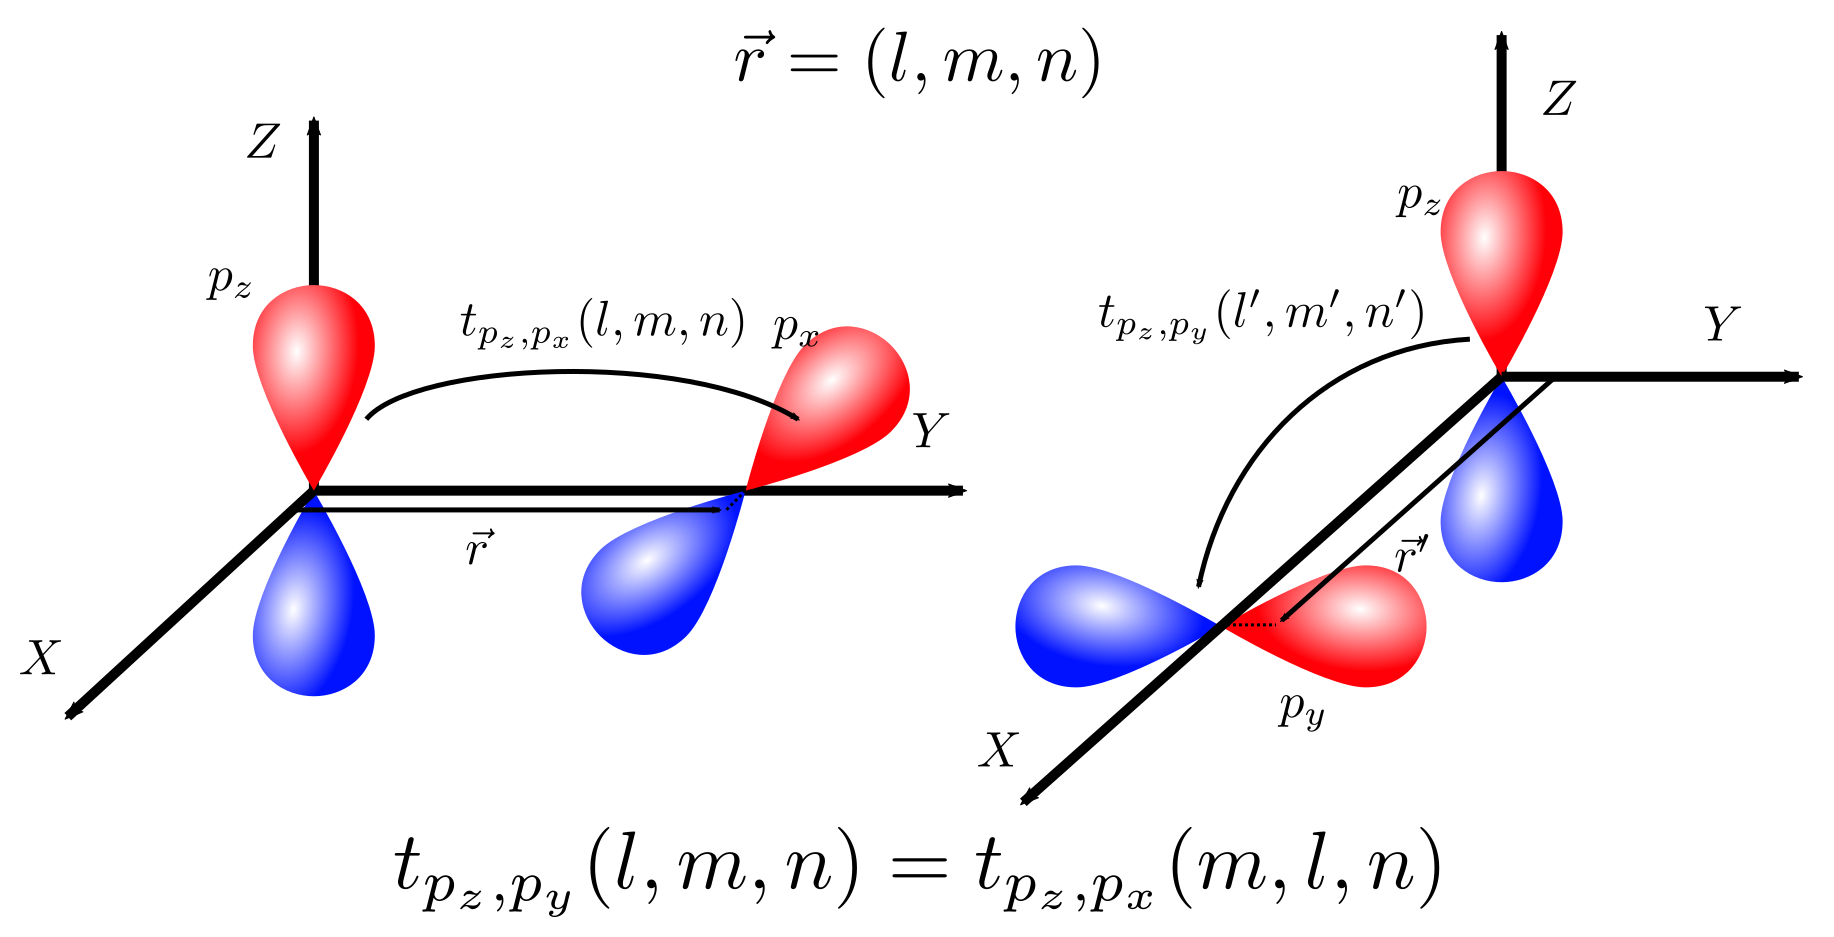
\includegraphics[width=0.45\textwidth]{SK.pdf}
%   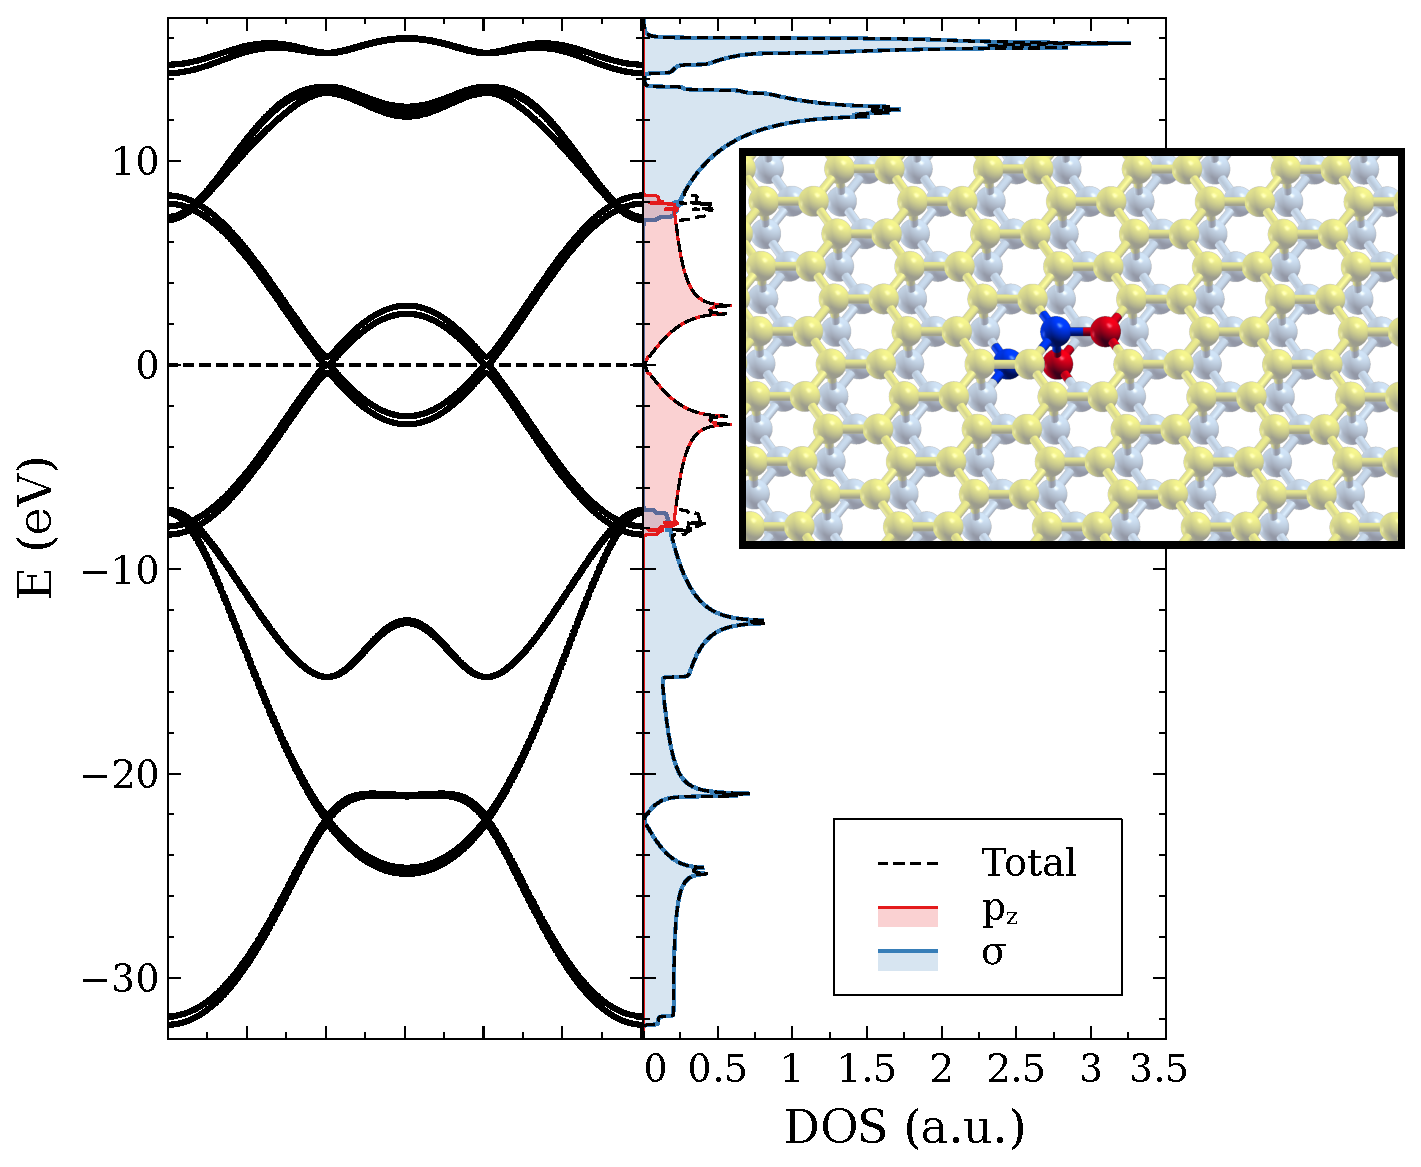
\includegraphics[width=0.45\textwidth]{bilayer_bandDOS.pdf}
% \vspace{-5pt}
% \caption{a) Panel show All the possible interlayer hoppings in graphene bilayer. b) Band structure and density of states of graphene bilayer}
% \label{hoppings}
% \end{figure}
% \FloatBarrier
% %~~~~~~~~~~~~~~~~~~~~~~~~~~~~~~~~~~~~~~~~~~~~~~~~~~~~~~~~~~~%
\subsection{Electric field}
% The band structure of graphene bilayer in such a model is shown in \ref{hoppings}.
The effect of an electric, $\Delta_E$ is to shift the energies of all the orbitals by an amount $\pm\Delta_E$, depending on the layer. This shift opens a gap in the Dirac Points. In nanoislands it can be seen that the gap opens linearly (for low field) with the electric field.

%~~~~~~~~~~~~~~~~~~~~~~~~~~ FIGURE ~~~~~~~~~~~~~~~~~~~~~~~~~%
\begin{figure}[h!]
  \centering
  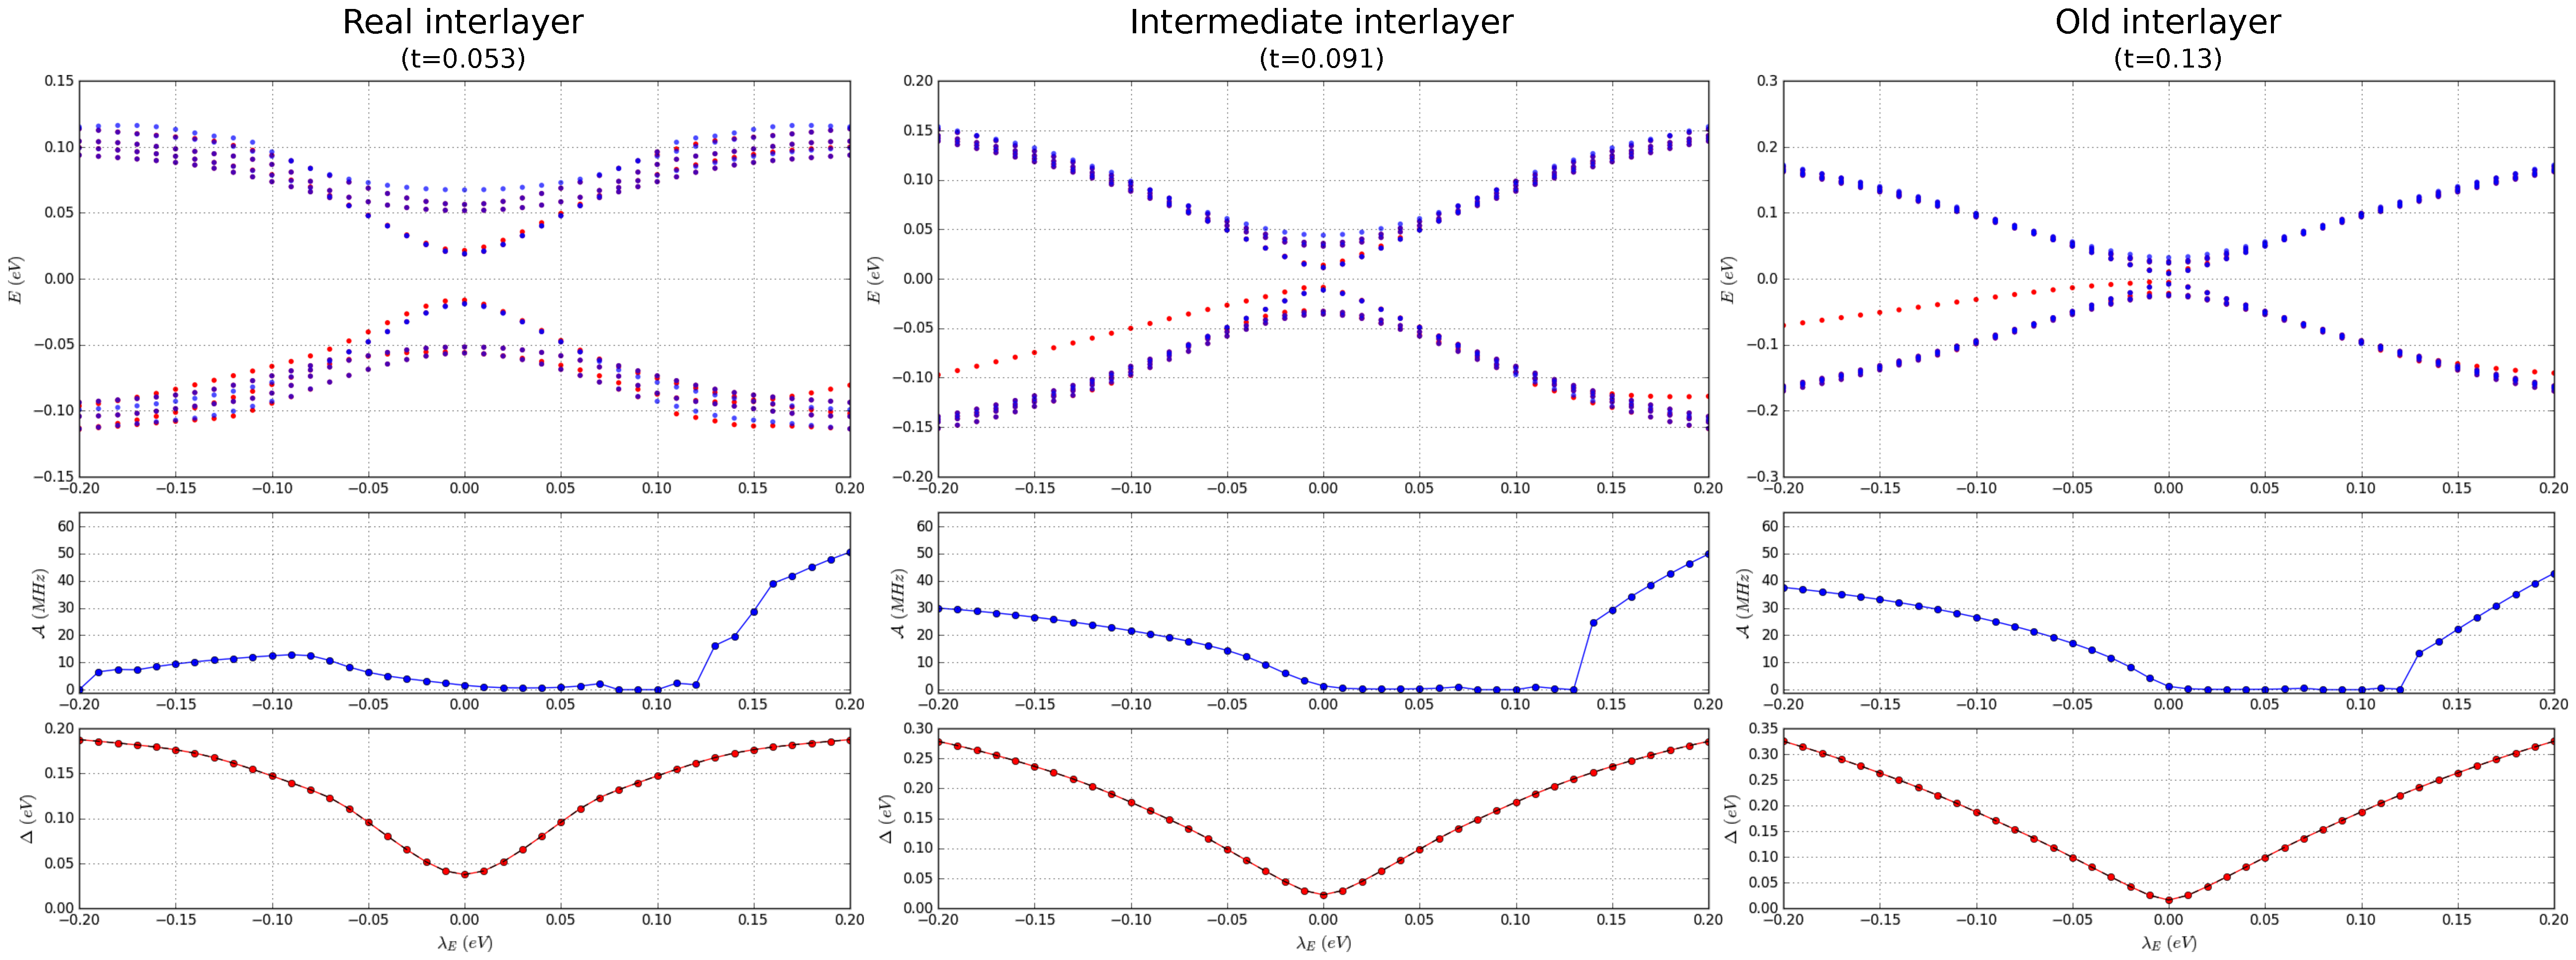
\includegraphics[width=\textwidth]{defects/fig/interlayer_elec.pdf}
  \vspace{-5pt}
\caption{Evolution of the low energy spectrum (the 8 eigenvalues closest to $E=0$), the hyperfine coupling and the gap with the electric field for different interlayer couplings. In the first panels the blue dots are the spectrum for the pristine island, without $H$ adatom and the red one is the defected case.}
\label{spectrums}
\end{figure}
\FloatBarrier
%~~~~~~~~~~~~~~~~~~~~~~~~~~~~~~~~~~~~~~~~~~~~~~~~~~~~~~~~~~~%

Given an island of a certain size (within the shadowed region in Fig.~\ref{confinement}) the evolution of the spectrum is shown in Fig.~\ref{spectrums}, Notice that the figure \emph{does not show bands} but rather discrete spectrums at different electric fields, in particular, the point at $\Delta_E=0$ \emph{is not the Dirac point}, it is simply the spectrum at zero electric field.

The main information that we can extract by now from Fig.~\ref{spectrums} is that the electronic structure of graphene bilayer opens a gap with the electric field.

The real value of the interlayer should be the one in the left panel, and it will be the one used from now on, meaning that \emph{the interlayer coupling will not be a free parameter in our calculations}.


\section{H adatom on graphene bilayer}

The physics of a $H$ adatom on bilayer graphene does not differ much from the monolayer case. In this case, again the Lieb's theorem nearly applies, although not exactly since the presence of $s$ orbitals break the bipartite character of the system.

To strictly recover the vacancy limit we would need to freeze the $s-s$ hopping ($V_{ss\sigma}\to0$) and increase the $s-p_z$ ($V_{sp\sigma}\to\infty$) as well as the on-site of the H atom ($\varepsilon_{H_s}\to-\infty$).

The effect of having finite hoppings and on-site energy is that the ``zero energy'' state is no longer at $E=0$.

%~~~~~~~~~~~~~~~~~~~~~~~~~~ FIGURE ~~~~~~~~~~~~~~~~~~~~~~~~~%
\begin{figure}[h!]
  \centering
  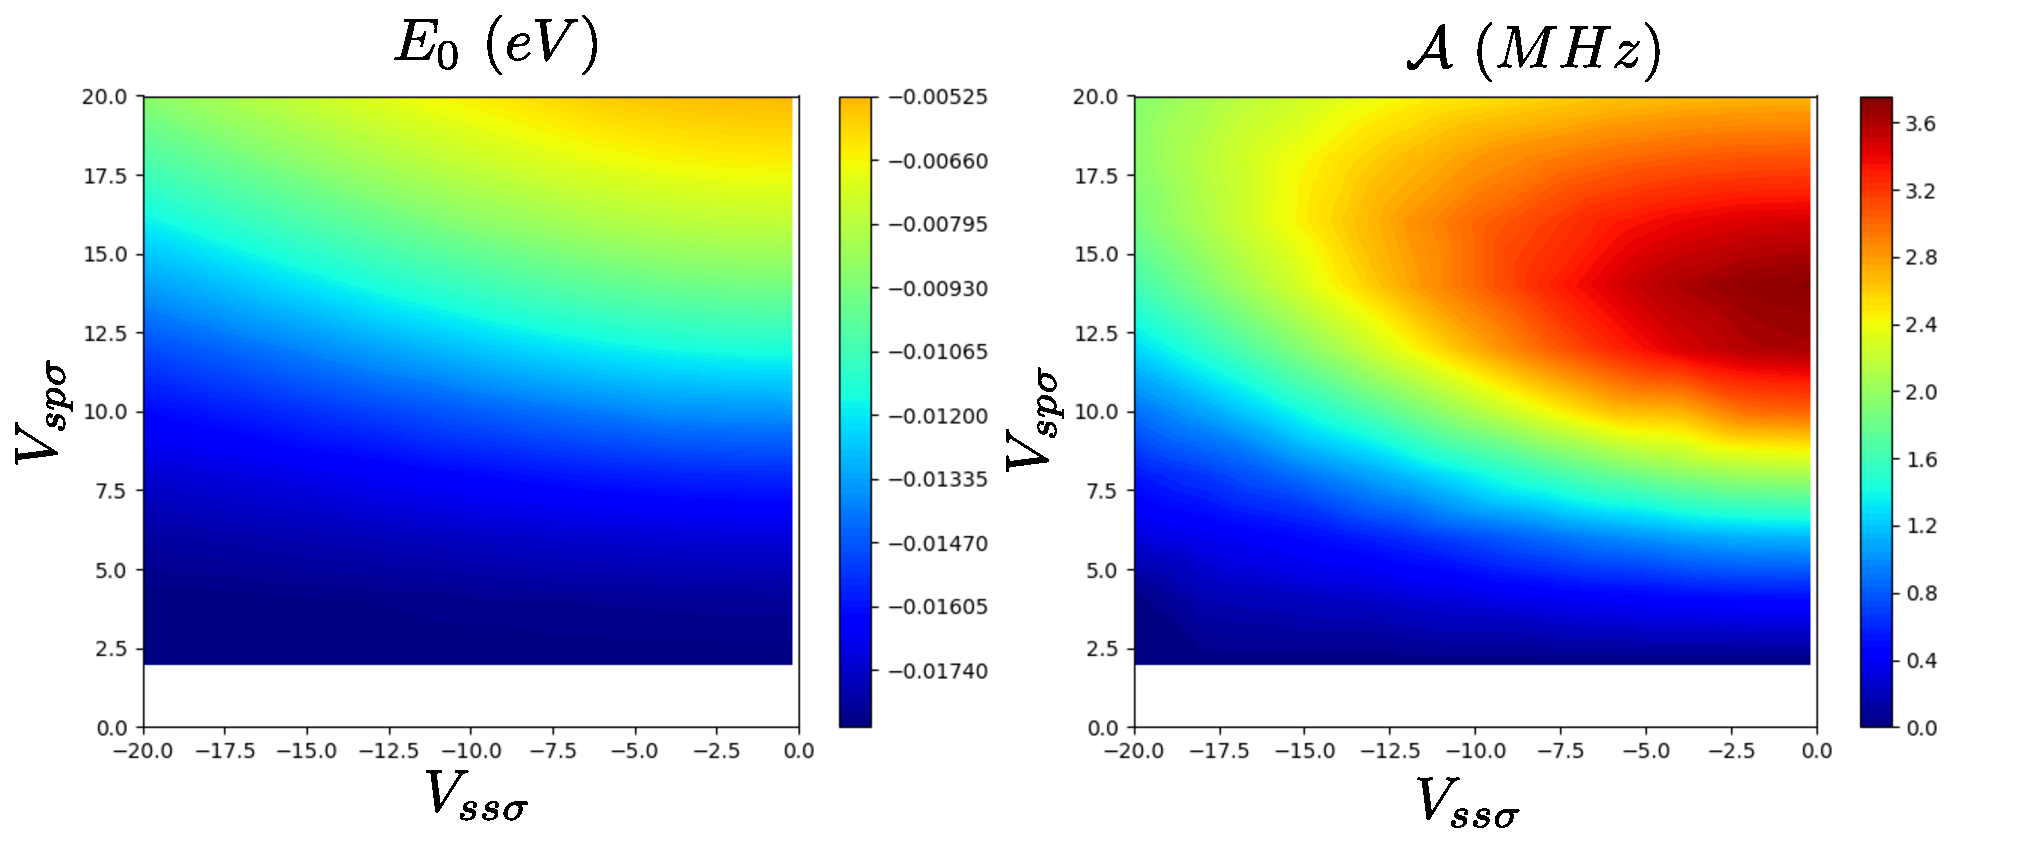
\includegraphics[width=0.9\textwidth]{defects/fig/parameter_space_bi.pdf}
  \vspace{-5pt}
\caption{Parameter space for the energy of the in-gap state and the hyperfine coupling for a graphene bilayer nanoisland.}
\label{SK2d_bi}
\end{figure}
\FloatBarrier
%~~~~~~~~~~~~~~~~~~~~~~~~~~~~~~~~~~~~~~~~~~~~~~~~~~~~~~~~~~~%

Notice that the parameter space $V_{ss\sigma}-V_{sp\sigma}$ looks quite similar to the monolayer case (Fig.~\ref{SK2d}) although there is a strong reduction in the hyperfine coupling $\mathcal{A}$ since the in-gap state is extended now among roughly twice as many atoms.\\


Choosing a value of  $V_{ss\sigma}$, $V_{sp\sigma}$ in the higest region in Fig.~\ref{SK2d_bi} we can see the evolution with the electric field:
%~~~~~~~~~~~~~~~~~~~~~~~~~~ FIGURE ~~~~~~~~~~~~~~~~~~~~~~~~~%
\begin{figure}[h!]
  \centering
  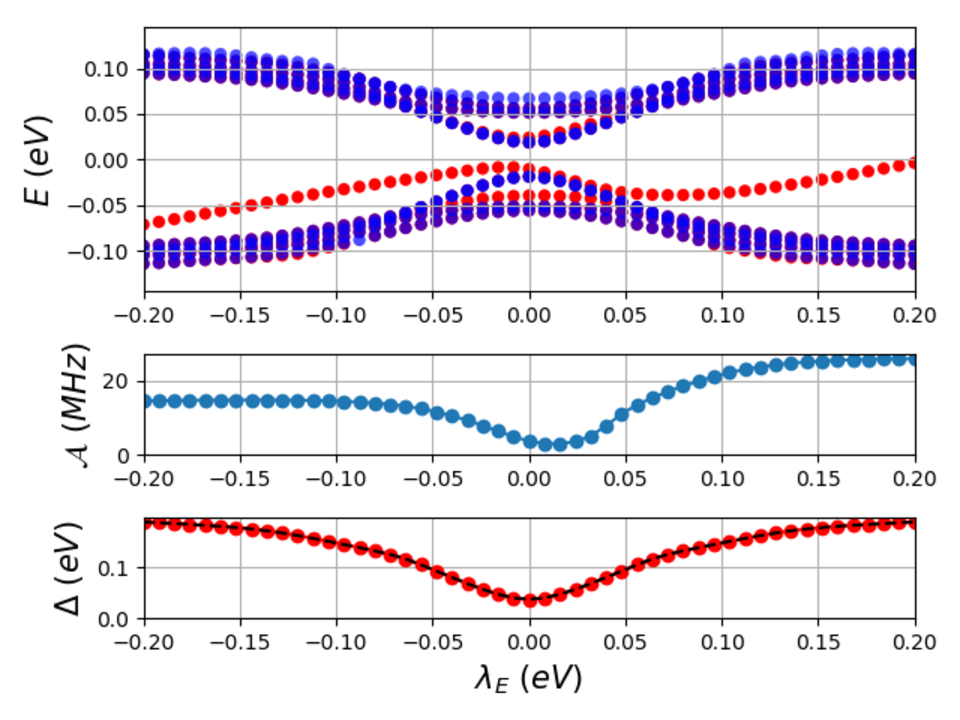
\includegraphics[width=0.6\textwidth]{defects/fig/best.pdf}
  \vspace{-5pt}
\caption{Evolution of the 8 eigenstates closest to $E=0$, the hyperfine coupling and the gap with the electric field}
\label{best}
\end{figure}
\FloatBarrier
%~~~~~~~~~~~~~~~~~~~~~~~~~~~~~~~~~~~~~~~~~~~~~~~~~~~~~~~~~~~%


And this is what the hyperfine coupling looks like in the parameter space $V_{ss\sigma}-V_{sp\sigma}$ when the electric field is switched on:
%~~~~~~~~~~~~~~~~~~~~~~~~~~ FIGURE ~~~~~~~~~~~~~~~~~~~~~~~~~%
\begin{figure}[h!]
  \centering
  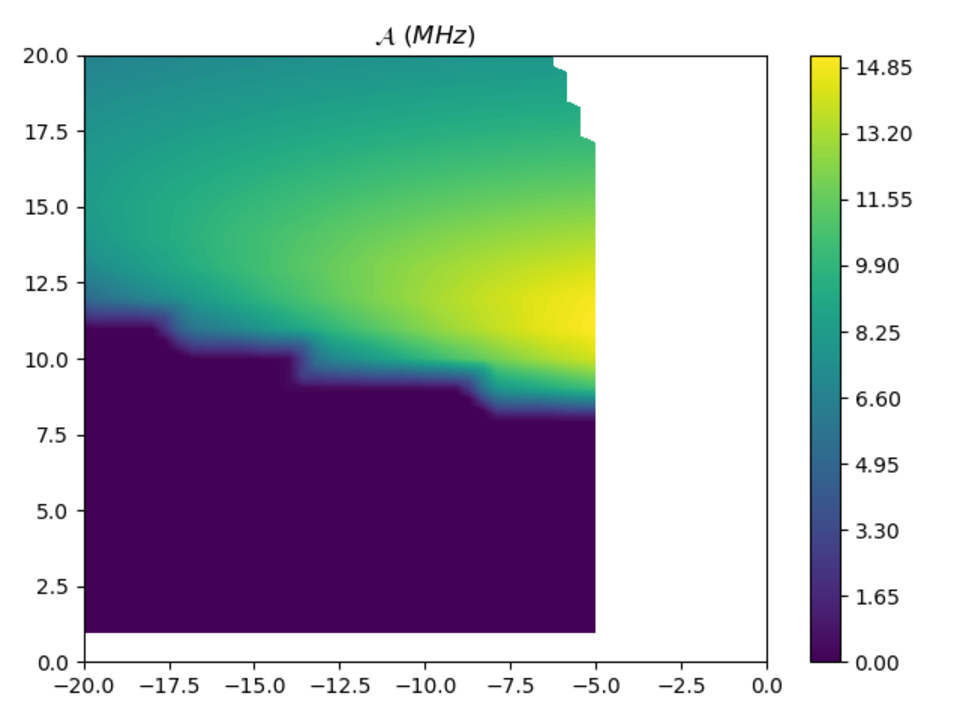
\includegraphics[width=0.6\textwidth]{defects/fig/SK_A_bi_e-02.pdf}
  \vspace{-5pt}
\caption{Parameter space for the hyperfine coupling for a graphene bilayer nanoisland in the presence of a strong electric field $\Delta_E=-0.2eV$}
\end{figure}
\FloatBarrier
%~~~~~~~~~~~~~~~~~~~~~~~~~~~~~~~~~~~~~~~~~~~~~~~~~~~~~~~~~~~%


%%~~~~~~~~ Chapter ~~~~~~~~
%\chapter{Artificial Lattices}
\section{Introduction [not serious]}
Theoretical Physicist have been dreaming with theoretical models since they realized it was much easier to write down and solve some equations than find a material governed by such equations. For years without end, we have created more and more models, useful, and boring, and silly, and interesting ones, but just theoretical models non the less.

The problem of vacancies/adatoms in graphene has been widely studied, both theoretically and experimentally. On one hand, the experimental studies usually focus on the local properties of the localized states, lacking the capability to study ``complex'' structures of vacancies/adatoms. On the other hand, theoretical studies usually relay on calculations in which the translational symmetry of the crystal is preserved, what is generally considered a handicap for the model since experimentally the vacancies do not form an array large enough to behave as a crystal. Any effect derived from the consideration of a crystal of vacancies is usually neglected either as an artifact of the theory or an unachivable experimental option. If this limitation is avoided, then the theoretical study focus in single vacancies as experimental studies usually do.

Recent experimental advances have shown the capability to arrange large areas/quantities of atoms with atomic precision\cite{Brihuega2016,Kalff2016}.
An obvious question is whether or not we can build artificial lattices by placing adatoms on graphene.

The idea is to use a large flake of graphene bilayer (the reasons will be explored later in the text) in which the adatoms are placed in very specific atomic positions to form a (periodic) crystal. Since graphene can be described with a triangular or a rectangular Bravais lattice, many crystals are available by choosing the suitable unit cell and lattice vectors.


There are two main reasons to choose graphene bilayer as the platform to build artificial fermion models. The first one is that graphene (and by extension graphene bilayer) is the most studied material ever. The fabrication and tuning capabilities exceeds those of any other material. The second one is that its electronic properties are highly tunable whether it is via proximity to other materials or via the application of external fields.

% XXX move
% When an external electric field is applied to graphene bilayer, a tunable gap is open\cite{Zhang2009,Lui2011,Ponomarenko2011} (the maximum observed value is $\Delta_E\sim\SI{0.25}{\eV}$).


\section{General considerations} %~~~~~~~~~~~~~~~~~~~~~~~~~~~~~~~~~~~~~~~~~~~~~%
We are going to study the electronic states arose by vacancies in the $\pi$-manifold in graphene bilayer (GB) and its interactions with an external electric field, $V$.
We will consider isolated vacancies in order to study the properties of the electronic states. Later on, we will also study infinite periodic arrays of defects forming a crystal.\\

When only a finite number of vacancies are considered, the system used will be an armchair island, as such, the system is $0$-D, so there is no translational symmetry and no $\vec{k}$ vector can be defined, nor Bloch's theorem can be applied.

To study these systems we will consider a basis of localized states that could be considered to be the $p_z$ hydrogenoid orbitals.
\begin{equation}
  \mathcal{B} = \left\{\phi_1,\phi_2,\dots,\phi_\alpha,\dots,\phi_{N_C}\right\}
\end{equation}

The general Hamiltonian will look like this:
\begin{equation}
  H = H_t + H_{t'} + H_{V}
\label{hamiltonian}
\end{equation}

The term $H_t$ represents the kinetic energy arising from the hopping between neighboring sites (intralayer), $H_{t'}$ represents the interlayer hoppings and the term $H_{V}$ corresponds to the effect of an external electric field on the electrons. Such a term is considered to be just a layer dependent shift in the on-site energies:
% \begin{equation}
%   H_{\lambda_E} = \lambda_E
%   \left(\begin{array}{cc}
%   \mathds{1} & 0 \\
%   0 & -\mathds{1}
%   \end{array}\right)
% \end{equation}
\begin{equation}
  H_{V} = V\lambda_l
\end{equation}
where $V$ is the potential difference between the two layers and $\lambda_l\in\{-1,1\}$ labels the layer.
The vacancies are introduced in this model as an infinite on-site energy for the chosen atom(s). Unless otherwise stated, everything is done in $eV$, \emph{not in hopping units}. The intralayer $p_z$-$p_z$ hopping is chosen as $t=\SI{-2.7}{\eV}$ and the interlayer $t'=\SI{0.4}{\eV}$ in accordance with the literature\cite{KatsnelsonBook}.\\

In the presence of vacancies, there will appear in-gap states (as many as vacancies are considered) which will be labeled by $\Psi_0$, $\Psi_1$, ... in order to distinguish them form any other eigenstate.
\begin{equation}
\begin{split}
  H\ket{\psi_\alpha} = E_\alpha\ket{\psi_\alpha} \qquad&;\qquad
\ket{\psi_\alpha} = \sum_\beta c_\beta\ket{\phi_\beta}\\
  H\ket{\Psi_0} &= E_0\ket{\Psi_0}
\end{split}
\end{equation}

\subsection{Graphene bilayer with an electric field}
The electronic structure of graphene bilayer in the presence of an external electric field has been widely studied. Here I summarize the basic relevant properties.\\
%~~~~~~~~~~~~~~~~~~~~~~~~~~ FIGURE ~~~~~~~~~~~~~~~~~~~~~~~~~%
\begin{figure}[!ht!]
\centering
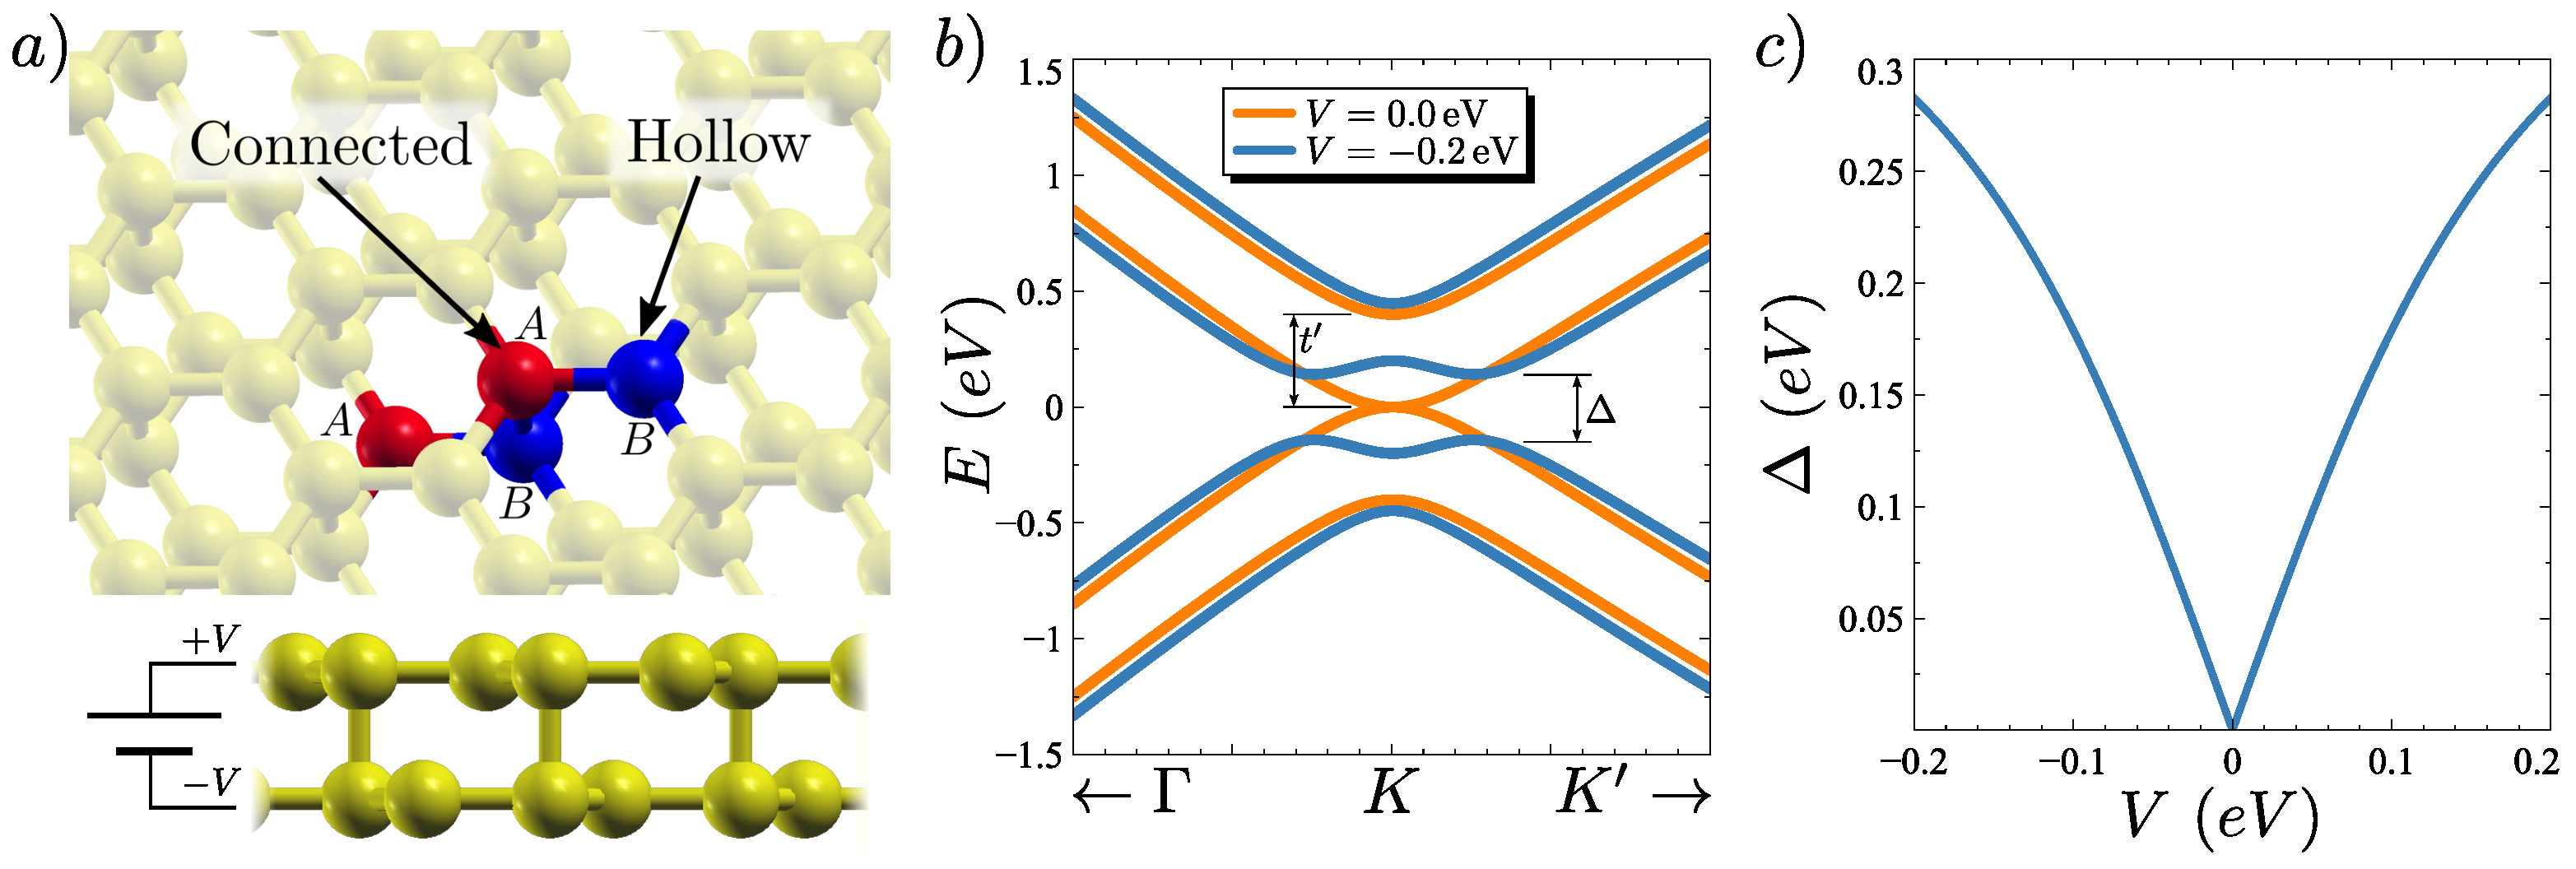
\includegraphics[width=0.9\textwidth]{artlat/fig/bands_bilayer.pdf}
\vspace{-5pt}
\caption{$a)$ Sketch of the minimal unit cell for graphene bilayer and disposition of the external electric field. Notice the two possibilities for placing the vacancies, we will focus on the hollow sites. $b)$ band structure of graphene bilayer with (blue) and without (orange) electric field. $c)$ Dependence of the gap open by the electric field. Notice that the gap is no longer at $K$, as shown in panel $b)$.}
\label{bilayer2d}
\end{figure}
% \FloatBarrier
%~~~~~~~~~~~~~~~~~~~~~~~~~~~~~~~~~~~~~~~~~~~~~~~~~~~~~~~~~~~%
Rather than having a linear band structure, graphene bilayer presents parabolic bands around the $K$ point. It has zero gap, and the next bands are split by $t'$. When an electric field is switched on, a gap is open at the $K$ point as shown in Fig.~\ref{bilayer2d}. The band gap behaves linearly for small electric fields.

This calculation is not exactly accurate with the experimental results\cite{Zhang2009} since it does not consider any self-consistent or screening effect at all, nevertheless it contains the necessary ingredients to describe the relevant physics of the problem, so for the sake of simplicity we will remain at this level of description.



\subsection{Vacancies in Graphene bilayer}
When a single vacancy is placed in graphene bilayer (or graphene, for that matter), the translational invariance is broken. For this reason, we consider a finite hexagonal island with armchair edges. In order to neglect the edge effects we will use nano-islands as big as $\SI{50.6}{\nm}$ in diameter (over 130K atoms). %131772 atoms)
As it is expected, in such a system the confinement gap decreases linearly with the area of the island (quadratically with the side), as shown in Fig.~\ref{confinement} $a)$. This model will break down when the scale of the electric field becomes comparable to the confinement gap. We shall, then, stay clear of the small electric field regime in order to avoid finite size effects. Depending on the calculation different sizes for the island can be chosen with no major consequences.
%~~~~~~~~~~~~~~~~~~~~~~~~~~ FIGURE ~~~~~~~~~~~~~~~~~~~~~~~~~%
\begin{figure}[!ht!]
\centering
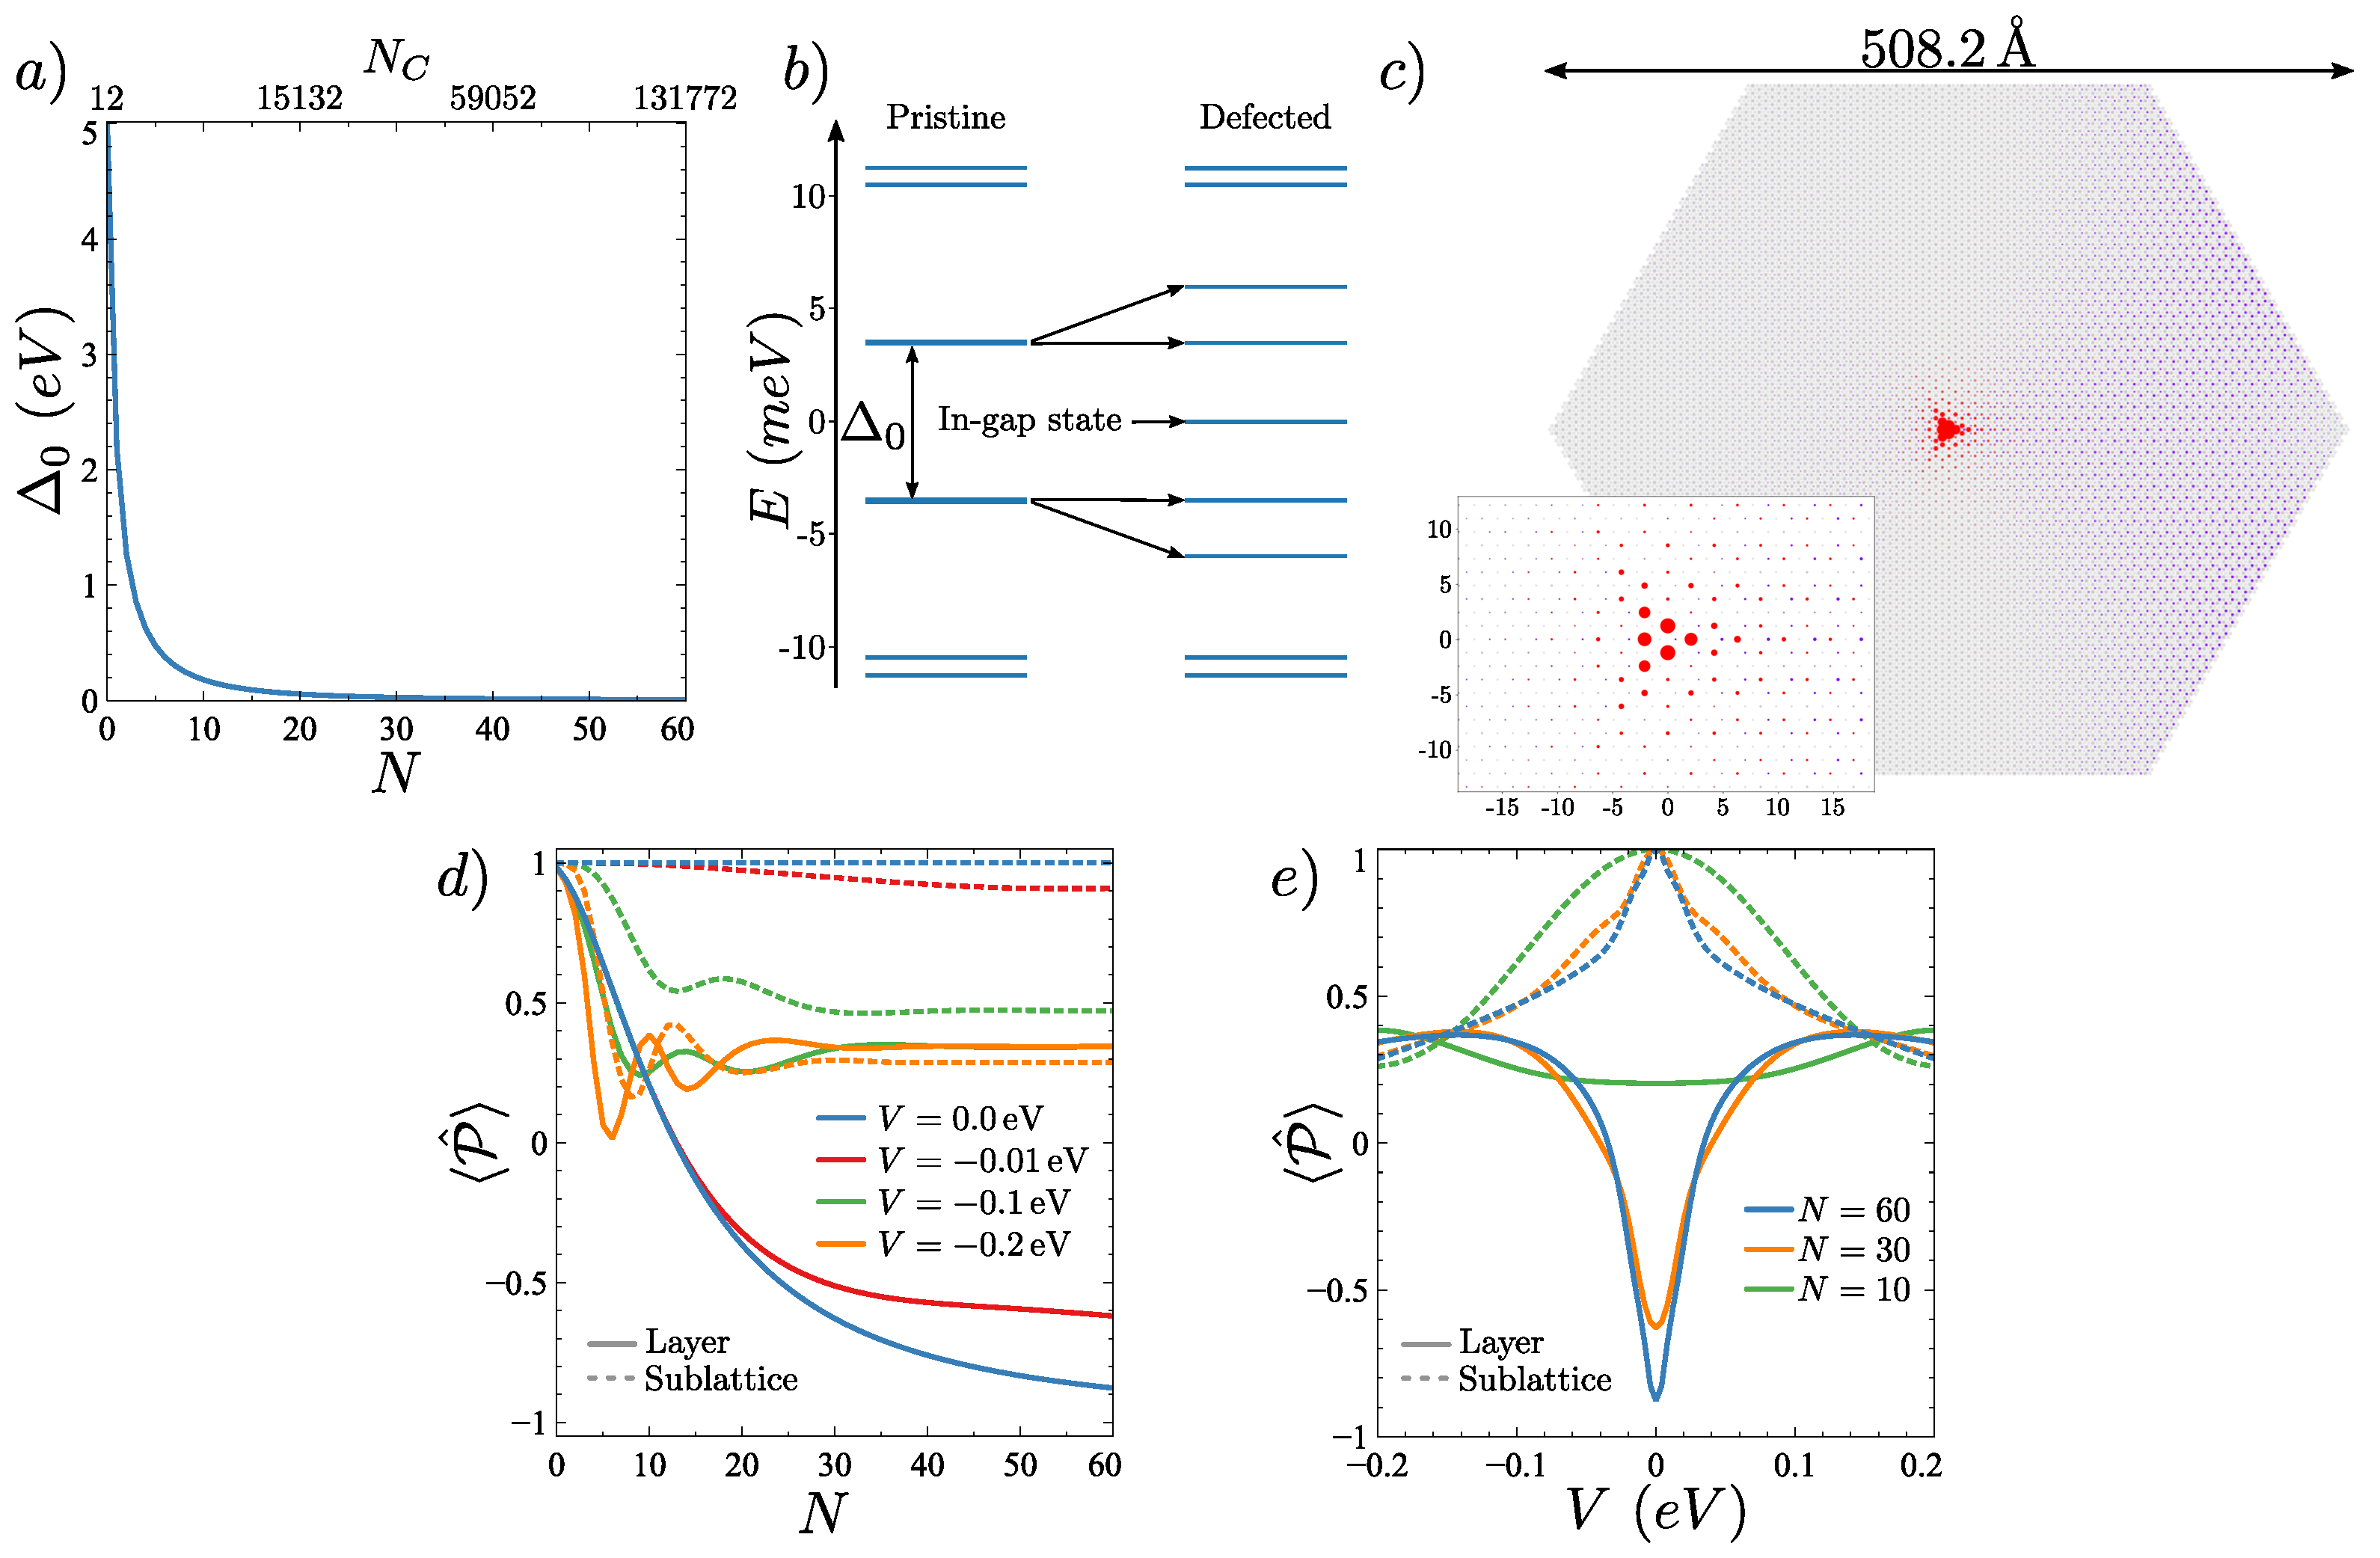
\includegraphics[width=\textwidth]{artlat/fig/confinement.pdf}
\vspace{-20pt}
\caption{$a)$ Confinement gap as a function of the size of the island (lower axis) and the number of carbon atoms $N_C$ in the island (upper axis). $b)$ Comparison of a pristine and a defected island, with a vacancy in the central hollow position. An in-gap state appears at zero energy. $c)$ Spatial distribution of the in-gap state. It appears distributed in both the top (red dots) and bottom layer (blue dots). Notice that the state is strongly localized around the vacancy in the top layer (red) while it is spread throughout the bottom layer (blue). The spatial distribution of the bottom layer is affected by the finite size of the sample and its exact shape is but a minor detail. The inset shows a $15\times\SI{10}{\angstrom}$ zoom of the in-gap state around the vacancy. $d)$ Dependence of the layer and sublattice polarizations with the size of the island. $e)$ Evolution of the layer and sublattice polarizations with the electric field for islands of different size.}
\label{confinement}
\end{figure}
% \FloatBarrier
%~~~~~~~~~~~~~~~~~~~~~~~~~~~~~~~~~~~~~~~~~~~~~~~~~~~~~~~~~~~%

We can calculate the spectrum of the system with and without a vacancy in order to compare both of them. Of course the full diagonalization of a $131772\times131772$ Hamiltonian is, at the very least, challenging for any standard computer, so we will use Lanczos diagonalization\cite{Lanczos1950, Ojalvo1970, Arnoldi1951} to obtain only the 9 eigenvalues closest to the Fermi energy.

As shown in Fig.~\ref{confinement} $b)$ the main difference when the vacancy is introduced is that a state appears in the middle of the (confinement) gap. As a matter of fact there will appear as many in-gap states as vacancies are introduced.

When we analyze the in-gap state we see that it is $100\%$ sublattice polarized, as predicted by the Lieb's theorem\cite{Lieb1989}. Regarding the layer distribution, it is distributed in both layers but not equitably. Interestingly, the in-gap state has more spectral weight in \textbf{the layer that does not host the vacancy} and the bigger the island, the stronger this polarization is as shown in Fig.~\ref{confinement} $d)$.
We can check the spatial distribution of this state (see Fig.~\ref{confinement} $c)$) to see that it is actually quite localized in the top layer (red dots), but completely spread over the bottom layer (blue dots). The particular shape of the distribution of the bottom layer is strongly affected by the edges so it is not to be considered as a reliable result, nevertheless its spreading (calculated via $IPR$ later) is consistent through different shapes and island sizes, and in accordance to the literature\cite{Castro2010}.

%TODO discuss <S> with size

\subsection{Note on the geometry}
All the vacancies considered will always be chosen on a hollow position (see fig~\ref{geo_sketch} $c)$) even if it not specified in the text. The behavior of vacancies in connected sites is studied somewhere else\cite{Castro2010}.

When only one vacancy is considered, it will be placed at the (hollow) atomic position closest to the center of the island in order to maximize the distance to the edges.

When two vacancies are considered, they will be placed as separated as possible from the edges, as shown in Fig.~\ref{geo_sketch} $b)$. This configuration (rather than placing one in the center, for instance) allows the study of a wider range of the angle, $\alpha$ and distance $d$.
When more than two vacancies are considered, they will be placed in the vertices of a regular polygon centered in the island.

% XXX For later, when talking about the angle
% Note that as long as the border effects are negligible, and due to the $C_3$ symmetry of the in-gap states in graphene, we only need to explore the range of angles between vacancies of $\alpha\in\left[0,60\right]$.

%~~~~~~~~~~~~~~~~~~~~~~~~~~ FIGURE ~~~~~~~~~~~~~~~~~~~~~~~~~%
\begin{figure}[h!]
\centering
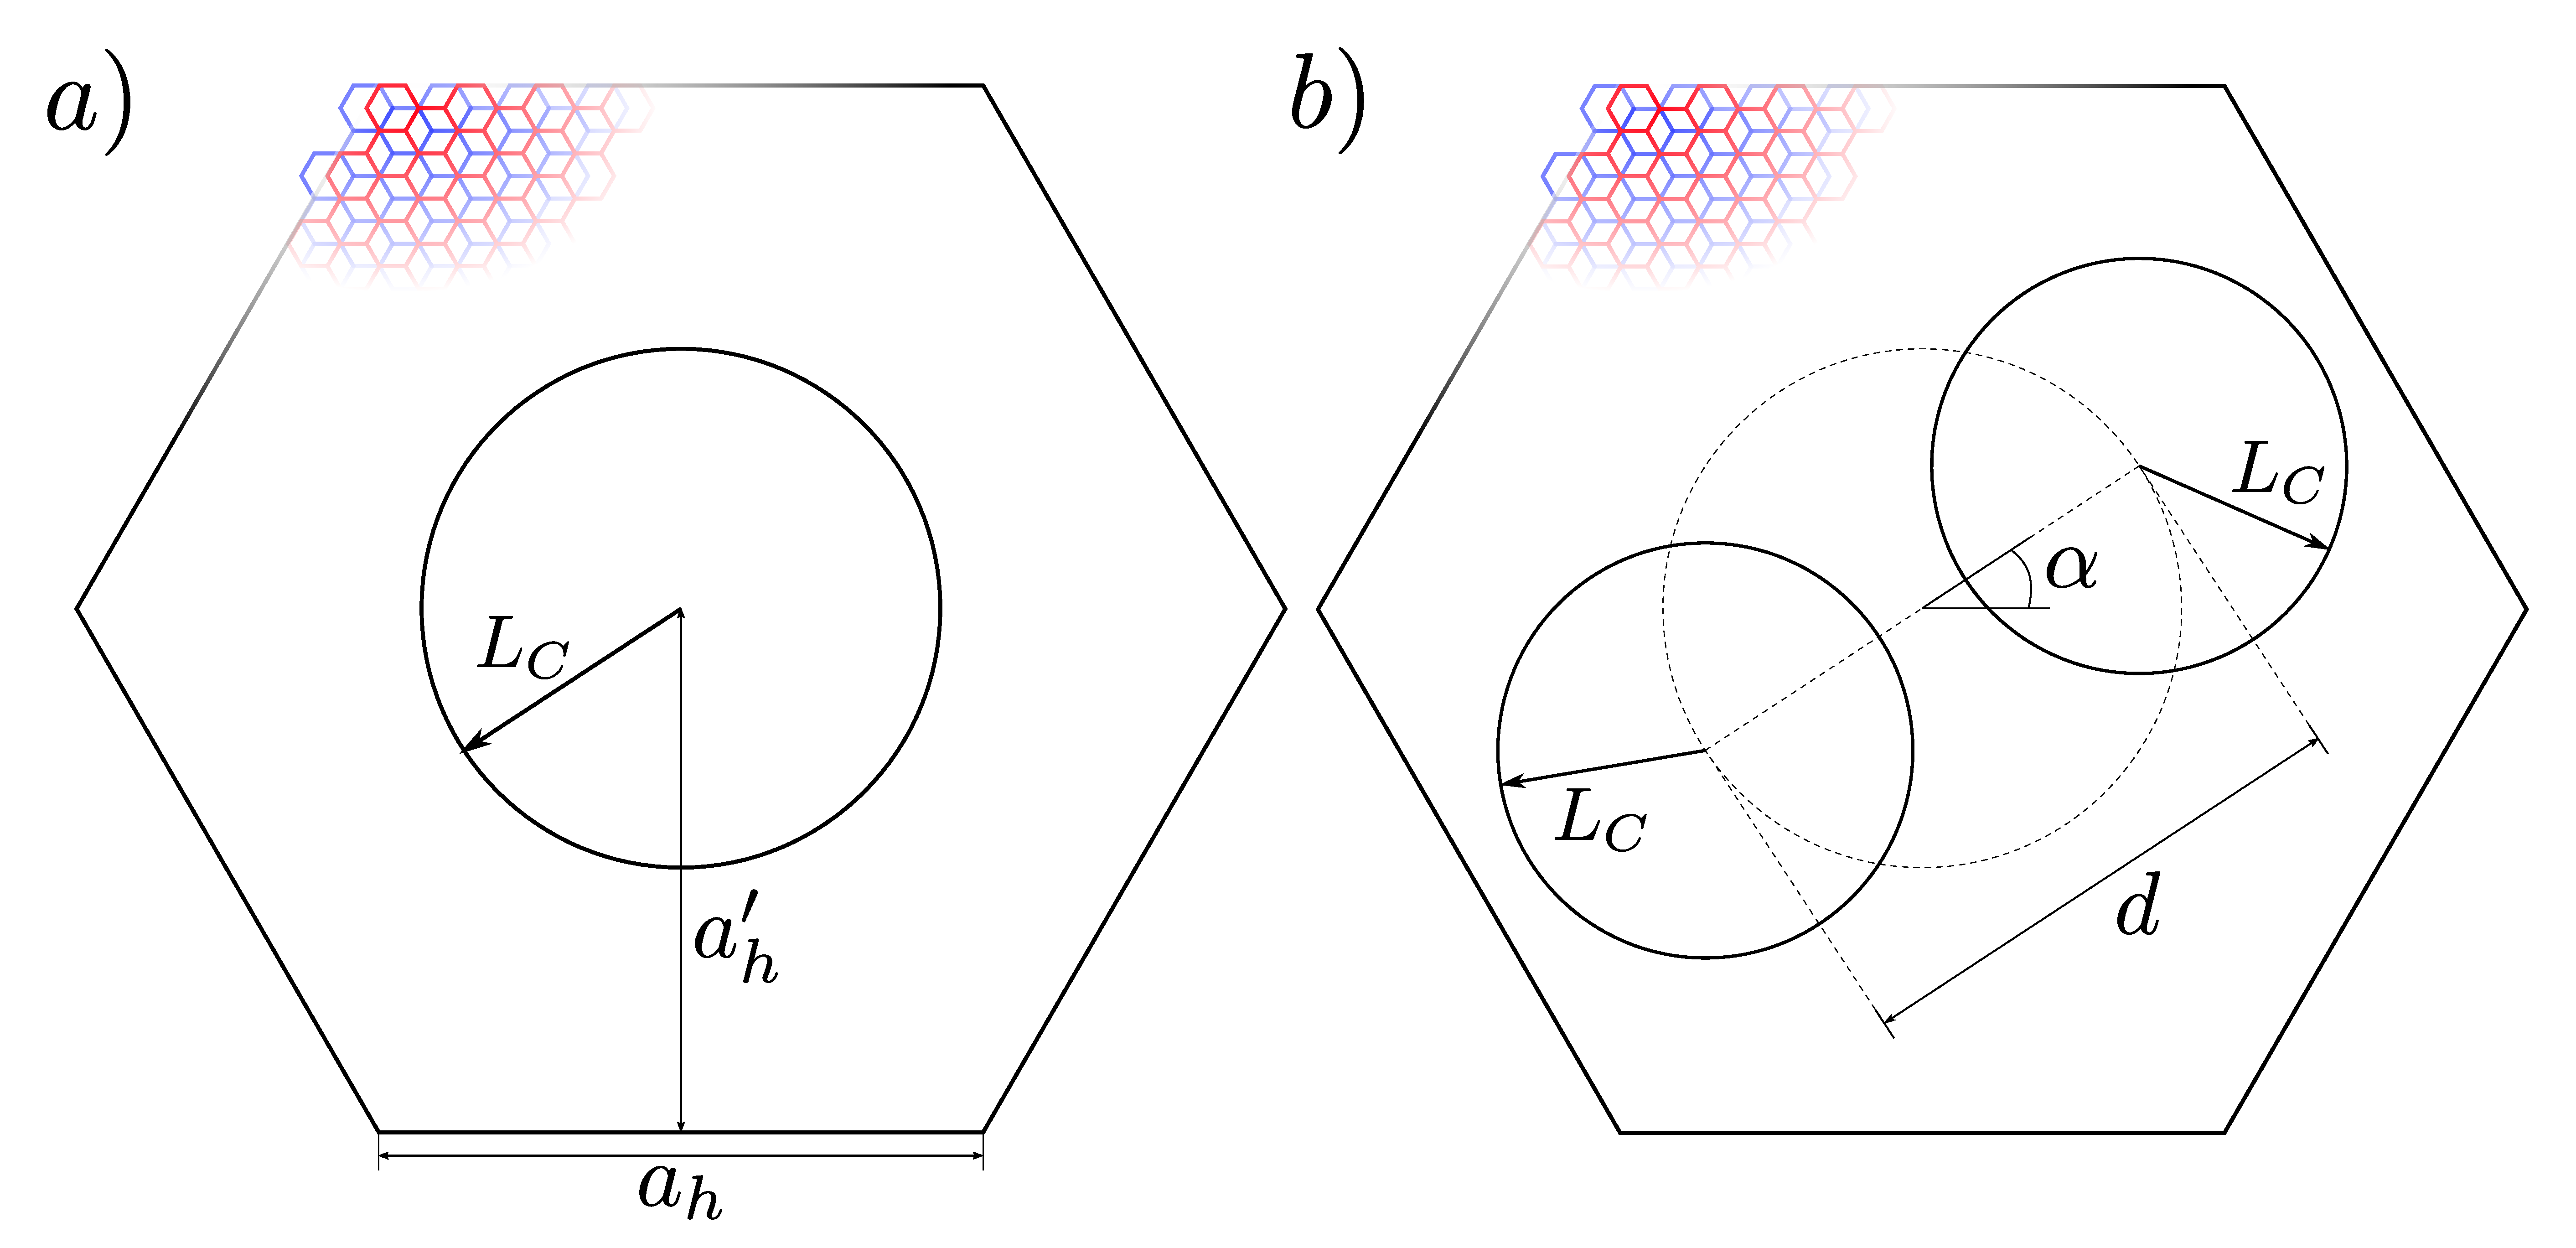
\includegraphics[width=0.7\textwidth]{artlat/fig/vacs_sketch.pdf}
\vspace{-10pt}
\caption{$a)$ and $b)$ show sketches of the position of the vacancies and relevant geometric information. In the upper left corner the real atomic structure is shown using blue for the lower layer and red for the upper one. The length $L_C$ is the typical size of the in-gap state.} % $c$ atomic structure showing the ``connected'' and ``hollow'' sites in the upper layer as well as the $A/B$ sublattices (in red/blue).}
\label{geo_sketch}
\end{figure}
\FloatBarrier
%~~~~~~~~~~~~~~~~~~~~~~~~~~~~~~~~~~~~~~~~~~~~~~~~~~~~~~~~~~~%




\section{0-D. Electric control of a single vacancy} %~~~~~~~~~~~~~~~~~~~~~~~~~~%
When an electric field is applied to bilayer graphene with a vacancy, the in-gap state will no longer be at zero energy. Instead, its position will shift with the electric field. As stated before, in a finite island we cannot define Bloch vectors, so we do not have bands. Nevertheless we can plot the spectrum of the island for different electric fields next to each other, this way we can have a band-looking plot showing the smooth evolution of the energy levels with the external potential.
%~~~~~~~~~~~~~~~~~~~~~~~~~~ FIGURE ~~~~~~~~~~~~~~~~~~~~~~~~~%
\begin{figure}[!ht!]
\centering
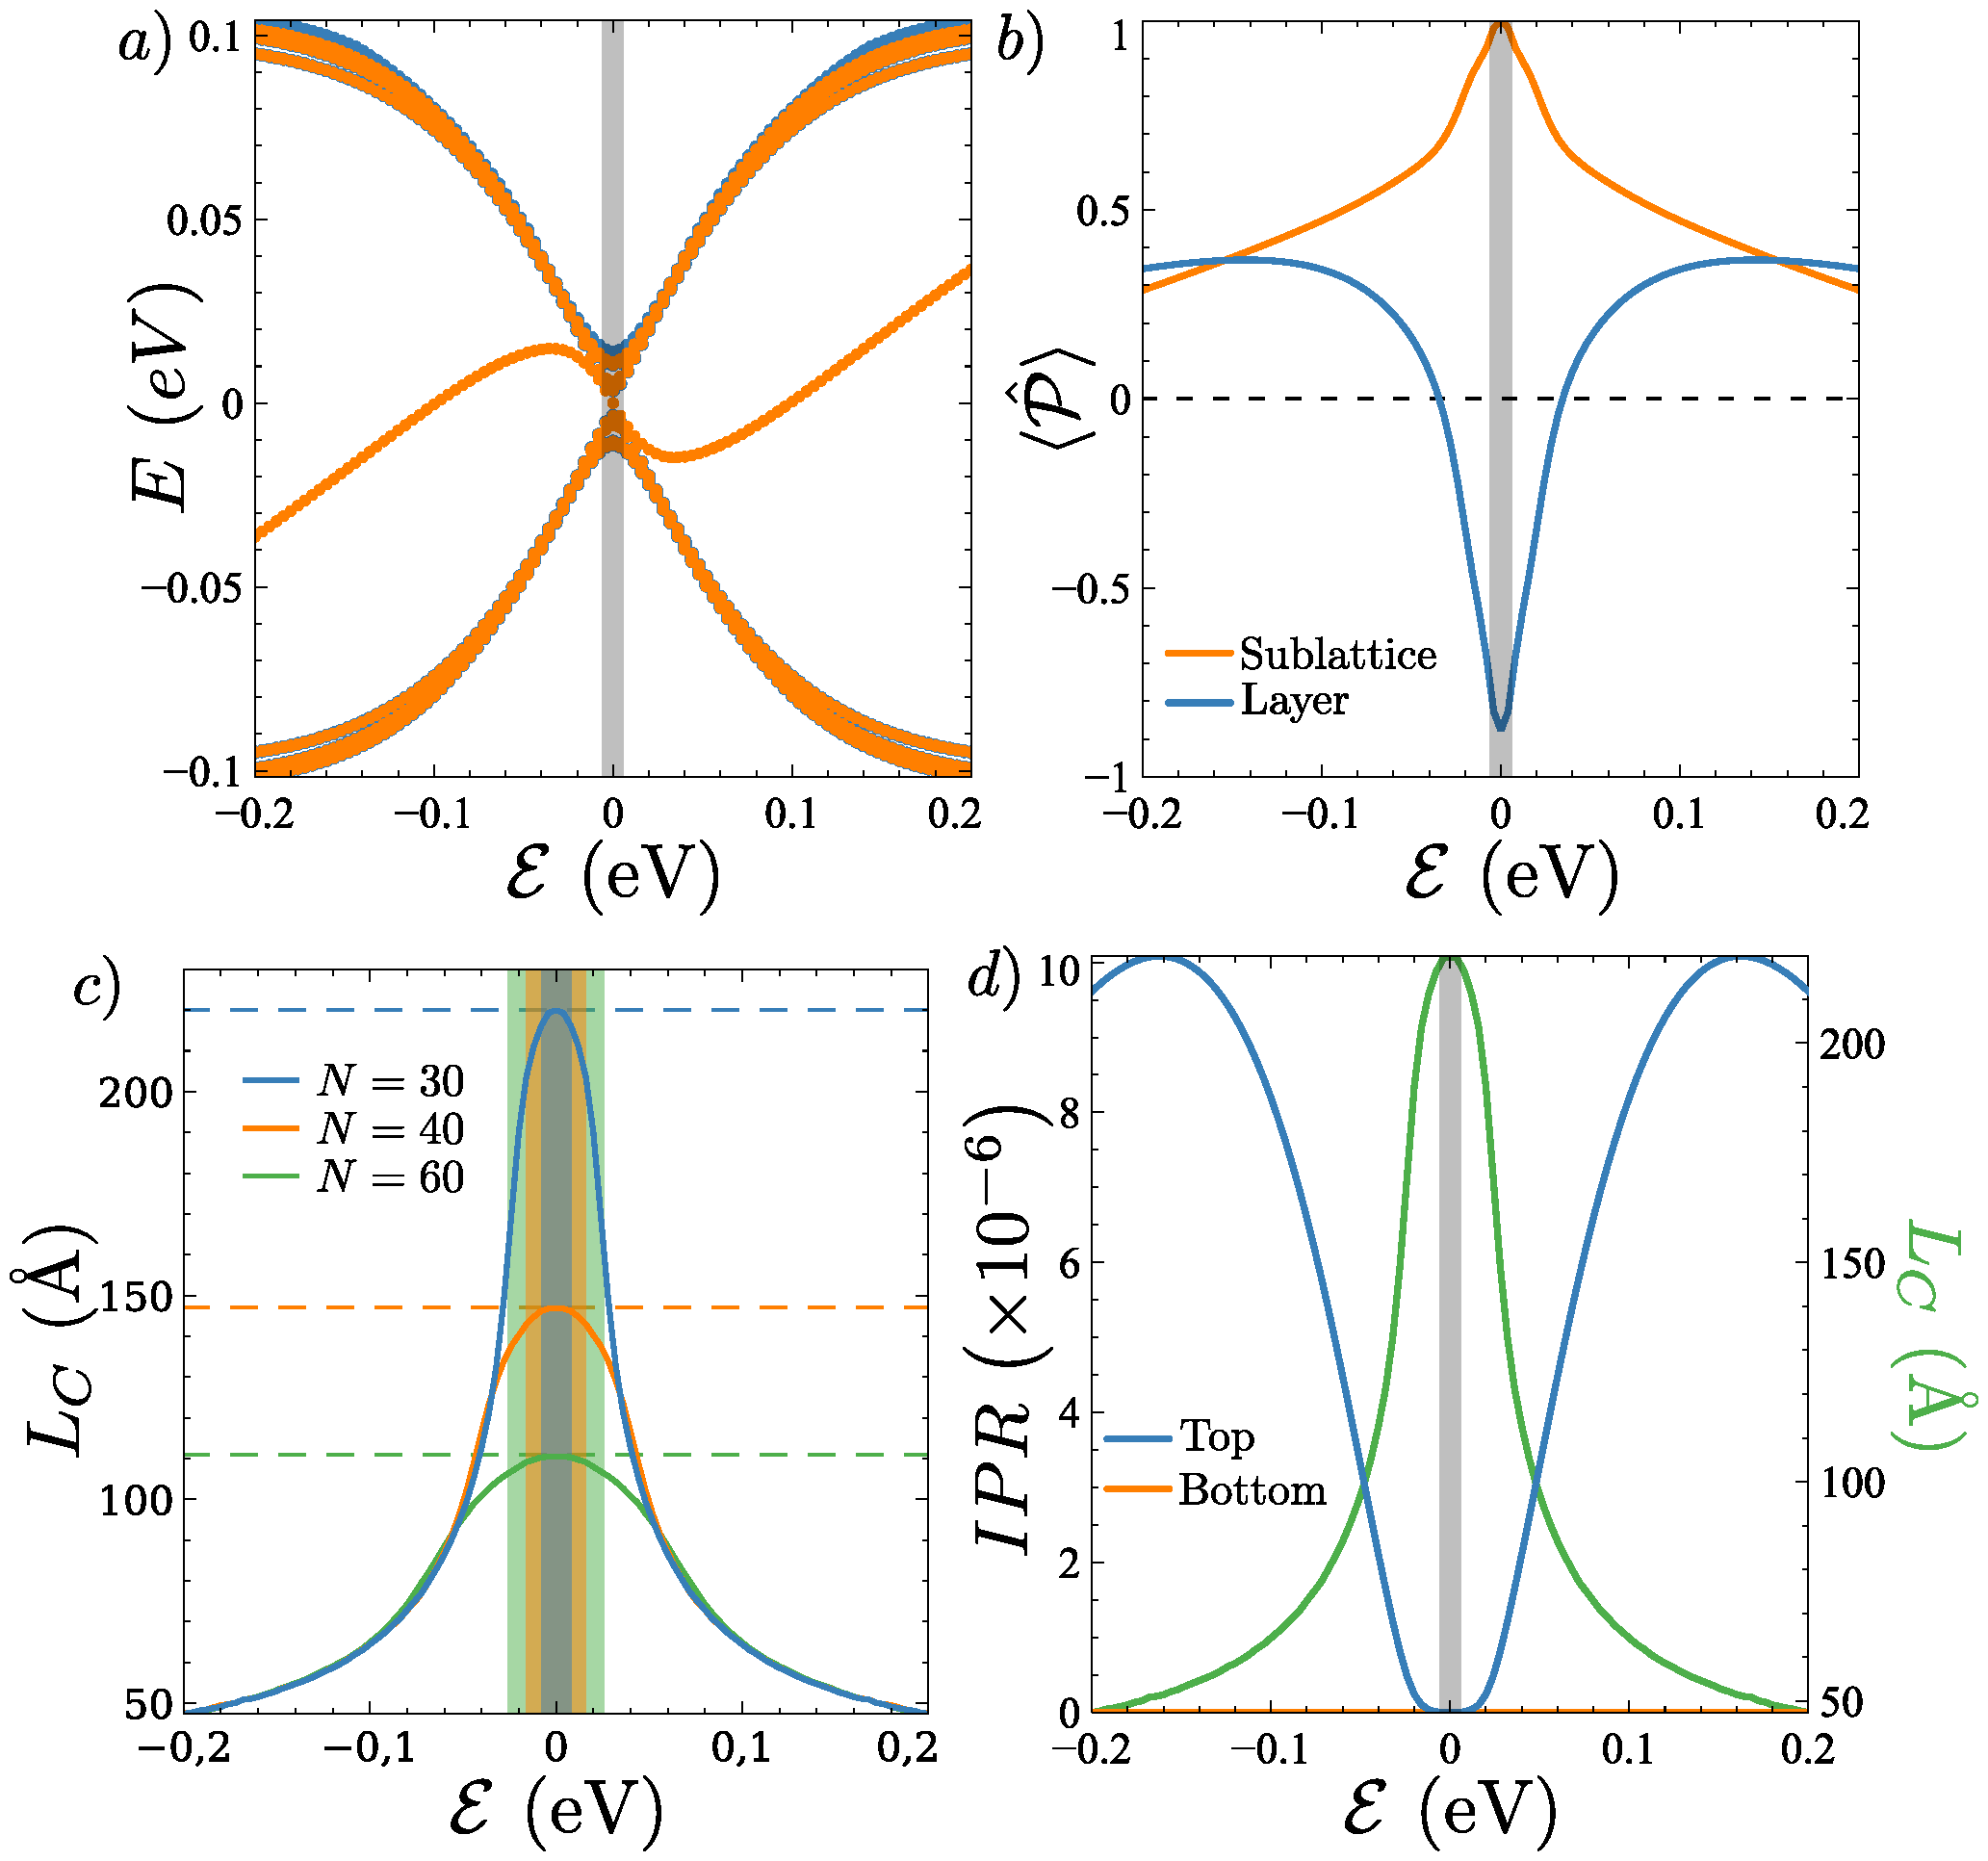
\includegraphics[width=\textwidth]{artlat/fig/spectrum.pdf}
\vspace{-20pt}
\caption{$a)$ Evolution of the spectrum of an armchair island with the electric field. $b)$ Sublattice and Layer polarization as a function of the electric field. $c)$ Evolution of the $IPR$ for the top (blue) and bottom layer (orange) and confinement length (green) with the electric field. Notice that the $IPR$ for the bottom layer is very close to zero ($IPR_b\sim10^{-11}$) while the for the top layer it changes five orders of magnitude with the electric field, showing how much the in-gap state can be confined. Analogously the confinement length shows (right axis) that the state is spread all over the island for $V=\SI{0}{\eV}$ but it can be confined to $\sim\SI{50}{\angstrom}$. The vertical gray strip in all panels shows the region where $|V|\leqslant\Delta_0$, where the edge effects can play a role.}
\label{spectrum}
\end{figure}
% \FloatBarrier
%~~~~~~~~~~~~~~~~~~~~~~~~~~~~~~~~~~~~~~~~~~~~~~~~~~~~~~~~~~~%
In Fig.~\ref{spectrum} we see the evolution of different properties with the electric field. Panel $a)$ shows the deformation of the spectrum of the island with the electric field. The in-gap state appears consistently in the middle of the gap but its position does not change monotonously. There is an interplay between the charge polarization and the external electric field.
As the electric fields becomes stronger, we can see that the in-gap state looses its initial polarization, Fig.~\ref{spectrum} $b)$, reaching a stable distribution of between both layers and sublattices. Another effect introduced by the electric field is the localization of the state. Fig.~\ref{spectrum} $c)$ shows the strong reduction of the confinement length, $L_c$, defined as:
\begin{equation}
  0.9 = \int_{r_0}^{L_C} \Psi_0(r) dr   %XXX arreglar!!!
\end{equation}
This non-standard definition gives an intuitive idea of how far from the vacancy (placed at $r_0$) is most of the state (over $90\%$ of it).
It is interesting to notice that the inverse participation ratio, $IPR$, defined as:
\begin{equation}
  \ket{\Psi_0} = \sum_\beta c_\alpha\ket{\phi_\alpha}\quad\quad;\quad\quad
  \text{IPR} = \sum_\alpha |c_\alpha|^4
\end{equation}
behaves quite differently for the top and bottom layer. Let us keep in mind that the smaller the $IPR$, the more spread the state is, in the limit case in which a given state is spread over all the $N$ available atoms, the $IPR$ would be $IPR=1/N$, while for a state localized in a single atom, it would be $IPR=1$.
For the bottom layer, the $IPR$ is very small and it barely changes with the electric field. This shows an extended state no matter the applied electric field. That is not the case for the top layer. In the top layer the $IPR\sim0$ for very small electric fields, but it increases rapidly with the electric field, showing that the state gets quickly localized. This is also confirmed by looking at the confinement length (green line in Fig.~\ref{spectrum} $c)$) which begins at a huge value, comparable to the size of the island, and decreases to a few nanometers.


A first order perturbative calculation of the energy at which the in-gap state should appear yields
\begin{equation}
  E_0 (V) = V \bra{\Psi_0}\hat{L}\ket{\Psi_0}
\end{equation}
In order to understand the implications of this, let us consider a vacancy in the upper layer ($\lambda_l=+1$). At $V=\SI{0.0}{eV}$, the in-gap state, $\Psi_0$, is quite layer-polarized: $\bra{\Psi_0}\hat{L}\ket{\Psi_0}\sim-0.8$. When the electric field is switched on, the in-gap state shifts with a negative slope. Nevertheless the electric field opposes the starting polarization and eventually they cancel out, which results in a change of sign in the slope. % XXX pufff.... rewritte

This behavior suggests a crossover between two interactions: the electric field and the kinetic terms. Let us study the effects of the interlayer coupling in this system.


\subsection{Role of the interlayer coupling}
Naively, one may expect the in-gap state to shift linearly with the electric field as, for instance, the conduction and valence states do. Nevertheless, the calculations show otherwise.
For small electric fields (we will discuss this scale later on) the in-gap state moves in opposition to the electric field, as discussed in Fig.~\ref{spectrum} $a)$.
%~~~~~~~~~~~~~~~~~~~~~~~~~~ FIGURE ~~~~~~~~~~~~~~~~~~~~~~~~~%
\begin{figure}[!ht!]
\centering
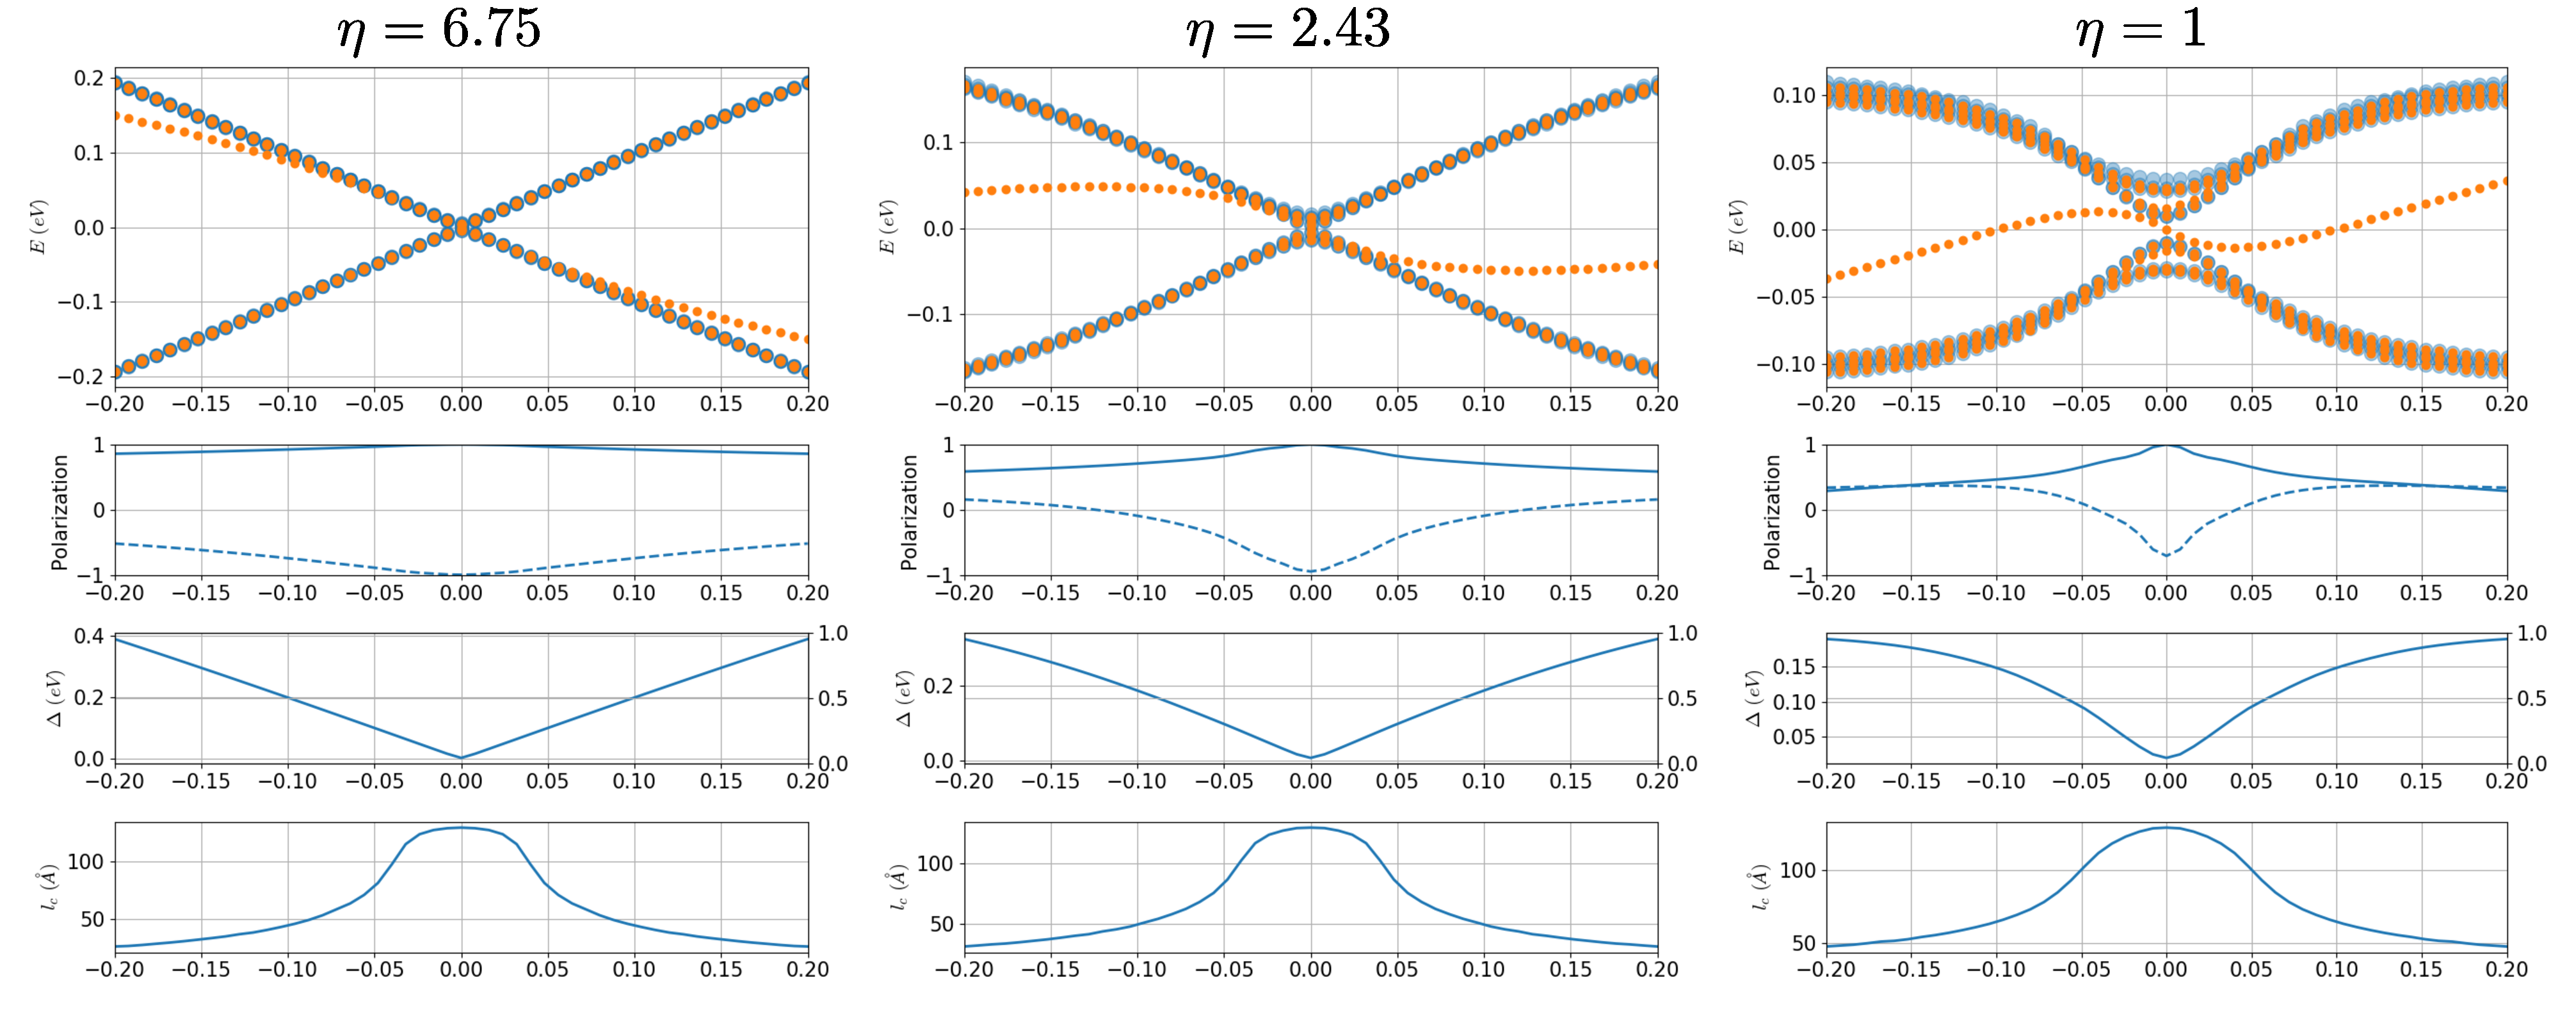
\includegraphics[width=\textwidth]{artlat/fig/ingap_interlayer.pdf}
\vspace{-15pt}
\caption{Evolution of the spectrum with the interlayer coupling. The left panel shows the spectrum if we consider interlayer interactions as strong as the intralayer ones. The right panel shows the realistic value and the central panel shows an intermediate situation.}
\label{ingap_interlayer}
\end{figure}
% \FloatBarrier
%~~~~~~~~~~~~~~~~~~~~~~~~~~~~~~~~~~~~~~~~~~~~~~~~~~~~~~~~~~~%
For large electric fields the in-gap state does move linearly with the electric field, yet, the rate at what it does depends strongly on the interlayer coupling, as shown in Fig.~\ref{ingap_interlayer}.
We will consider the Hamiltonian of the system to be two graphene hamiltonians coupled by an interlayer interaction:
\begin{equation}
  H = H_{\text{L}_1} + \eta H_{\text{inter}} + H_{\text{L}_2}
\end{equation}
The intralayer $\pi$-hoppings are $t=\SI{-2.7}{\eV}$ while the interlayer hoppings (which are $\sigma$-hoppings, due to the symmetry of the orbitals) are roughly $t_{\text{inter}}=\SI{0.4}{\eV}$. $\eta$ is an artificial adimensional parameter that will allow us to tune the interlayer coupling to study the behavior of the system. In this fashion, $\eta=1$ corresponds to normal, realistic GBL, while $\eta=0$ describes two decoupled graphene layers and, in particular, $\eta=6.75$ corresponds to having an \emph{inter}layer coupling as strong as the \emph{intra}layer one.\\

In order to understand the role of the interlayer coupling in the in-gap state, it is useful to plot the dependence of the layer polarization with the parameter $\eta$. We consider this parameter to range from 0.5 (slightly decouple) to 6.75 (strongly coupled so inter and intralayer hopping is the same).
%~~~~~~~~~~~~~~~~~~~~~~~~~~ FIGURE ~~~~~~~~~~~~~~~~~~~~~~~~~%
\begin{figure}[!ht!]
\centering
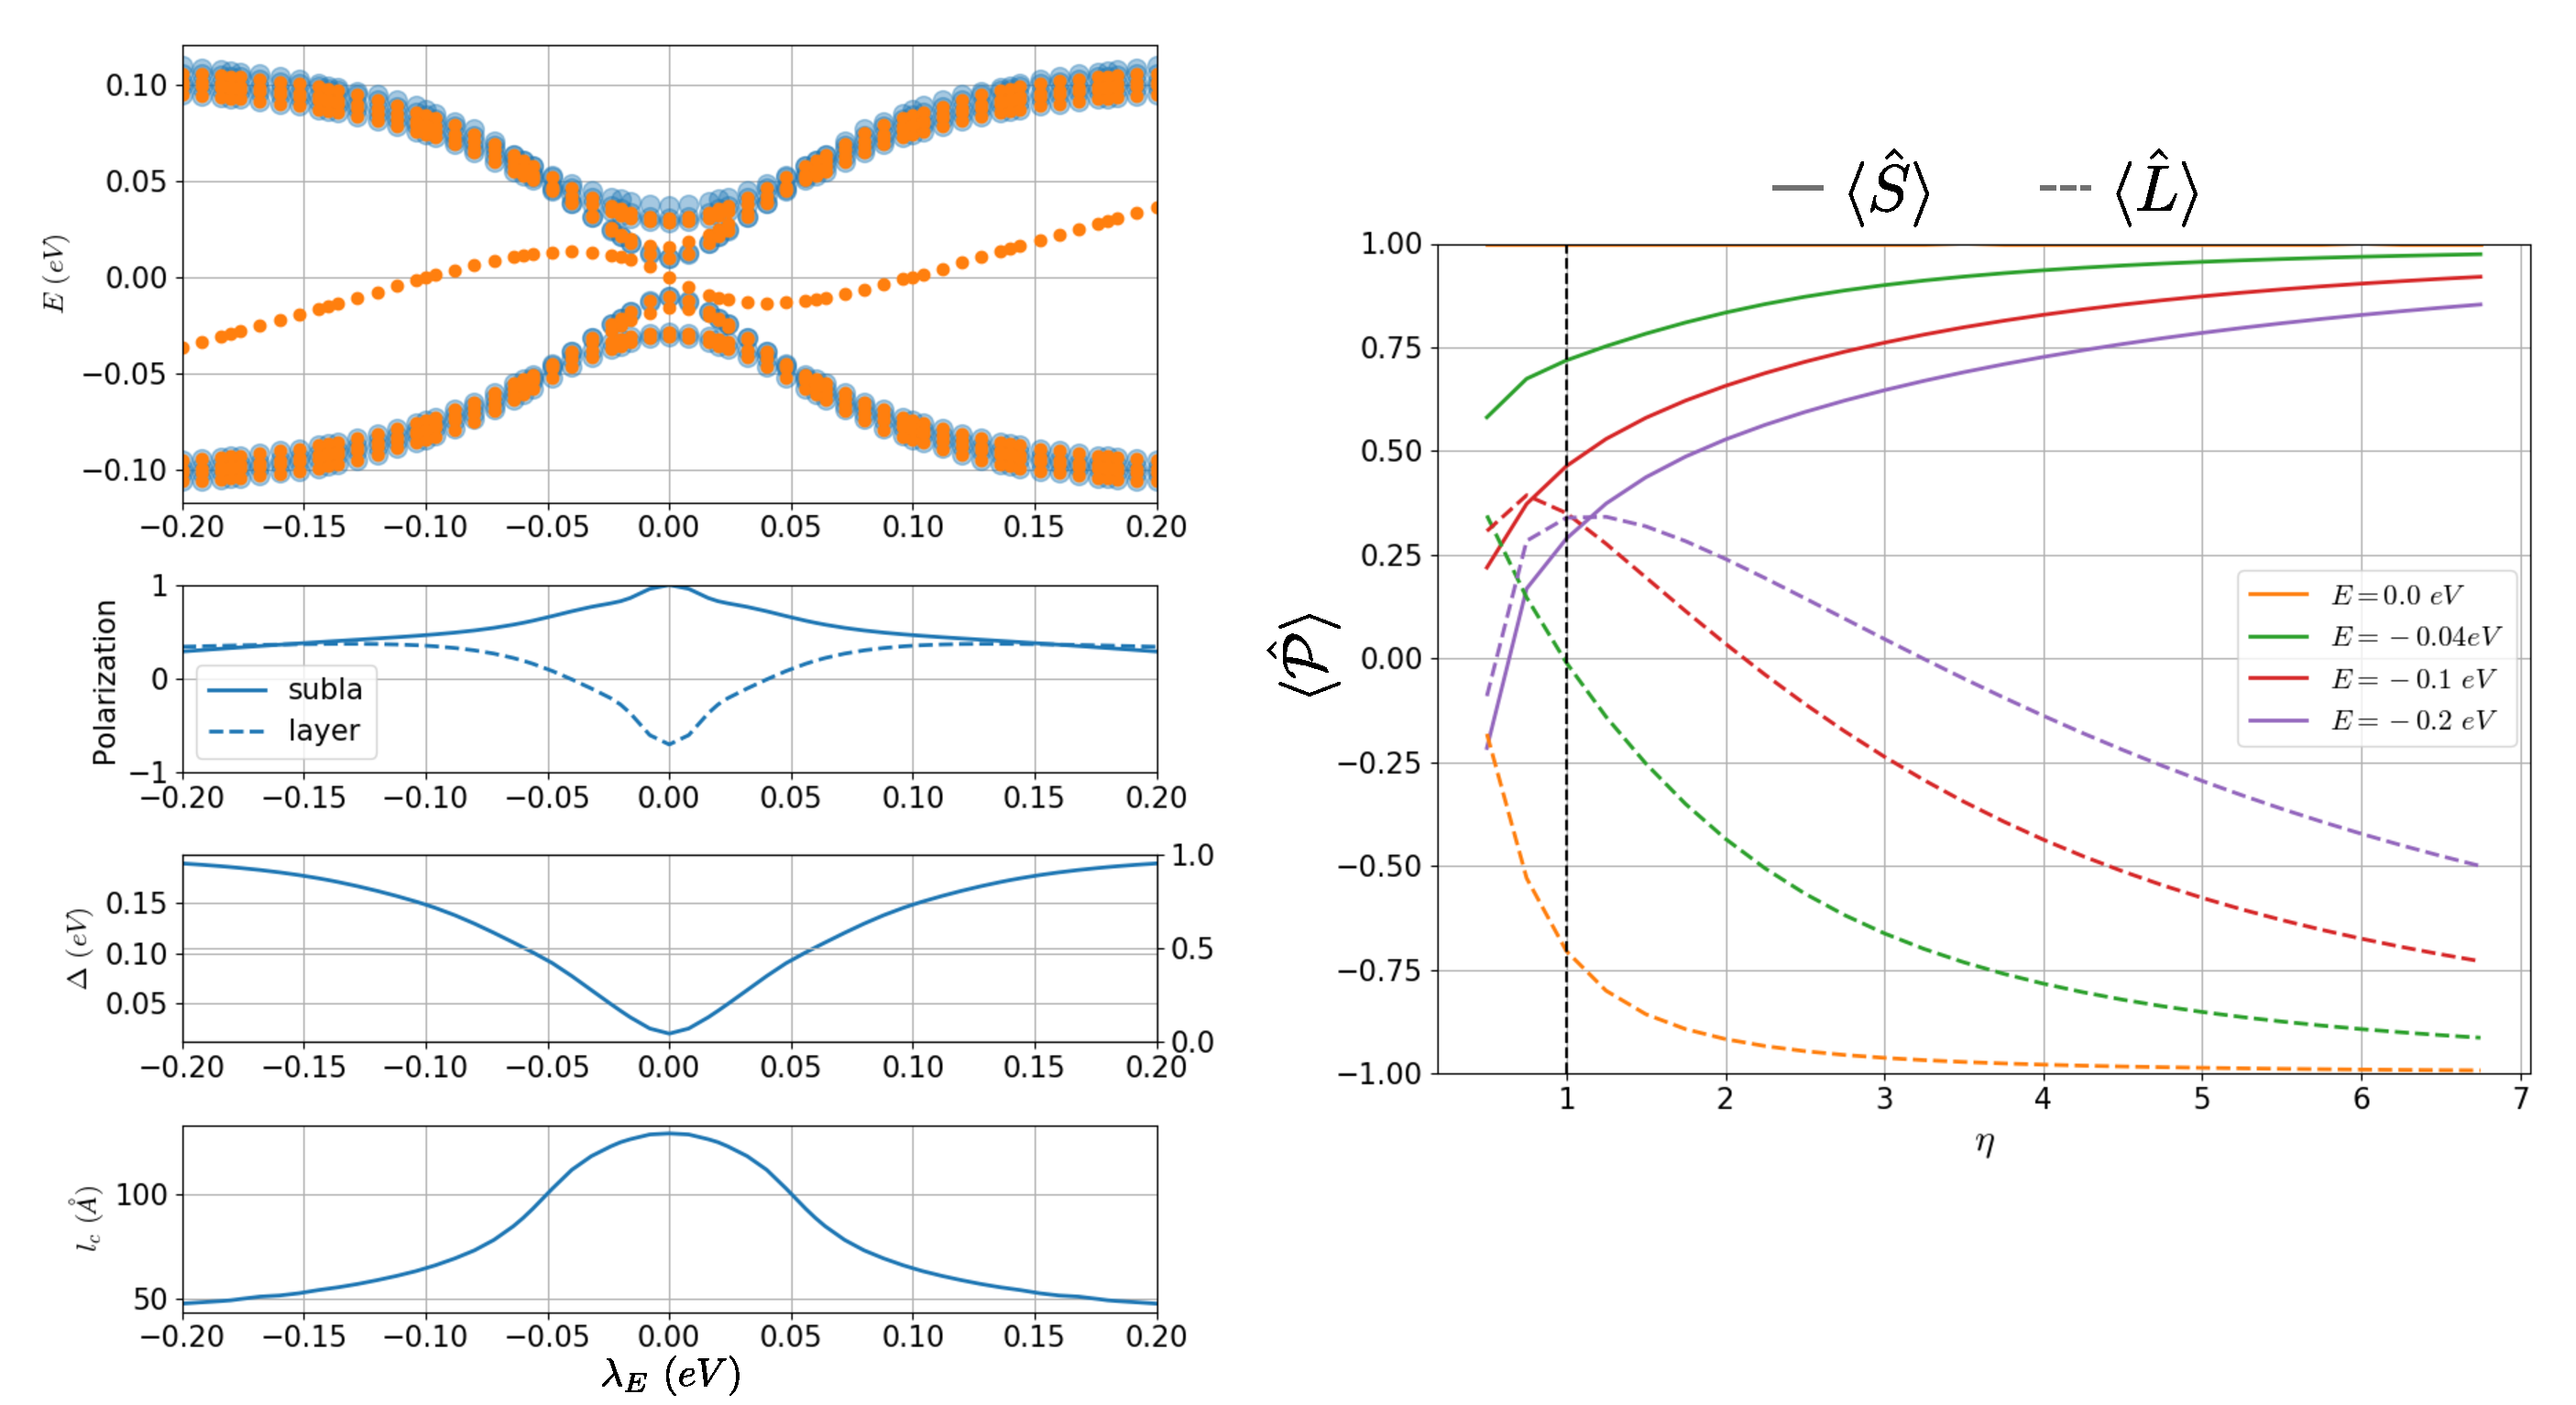
\includegraphics[width=\textwidth]{artlat/fig/polarization.pdf}
\vspace{-15pt}
\caption{$a)$ Evolution of different properties with the electric field. First panel shows the evolution of the spectrum, the second one shows the sublattice and layer polarizations, the third one plots the gap of the system and the forth one shows the confinement length. $b)$ Evolution of the layer (dashed lines) and sublattice polarization (solid lines) with the interlayer coupling. Notice that at zero electric field, $V=\SI{0.0}{\eV}$, the sublattice polarization remains constant at $\langle\hat{S}\rangle=1$, as expected from the Lieb's theorem.}
\label{pol}
\end{figure}
\FloatBarrier
%~~~~~~~~~~~~~~~~~~~~~~~~~~~~~~~~~~~~~~~~~~~~~~~~~~~~~~~~~~~%
We can see that the electric field overcomes the interlayer contribution when the system reaches charge neutrality $\langle\hat{L}\rangle=0$.

We can try to understand this step by step. When a H adatom is introduced (aka, a vacancy), one electron is localized in the vicinity of the defect. %The three closest atoms bear most of the spectral weight of this state, and the rest spreads all over the island but only in one sublattice.
For an adatom chemisorbed on top of a C atom belonging to the sublattice -1 in the top layer (namely 1), the sublattice and layer polarization are:
\begin{equation*}
  \langle\hat{S}\rangle = 1 \quad;\quad
  \langle\hat{L}\rangle = -0.7
\end{equation*}

This means that the in-gap state is completely sublattice polarized (as Lieb's theorem predicts) but it is only $\sim70\%$ layer polarized, meaning that the localized electron lives mostly \textbf{in the layer that does not contain the vacancy}.

If we artificially increase the value of the interlayer coupling we can that the layer polarization consistently drops to lower values, showing that the in-gap state prefers to spread in the layer that does not contain the vacancy. Analogously, the evolution of the sublattice polarization also shows that the in-gap state gets more and more sublattice-polarized.

This behavior might be understood keeping in mind the behavior of a single vacancy in graphene. It is known that for a vacancy in graphene, the in-gap state is mostly concentrated in the three closest atoms. In graphene bilayer it happens that these three closest atoms are connected to the other graphene layer, so the stronger the interlayer coupling, the easier will be for the in-gap state to spread to the other layer.

What I do not understand is that the 3 atoms closest to the vacancy (containing most of the state at $\eta=0$) are connected to atoms of the opposite sublattice in the other layer, yet, the sublattice polarization seems to keep its expected flavor even when the interlayer coupling is heavily increased.















% \newpage
% Since we are studying an island with a single vacancy, the energy levels are a discrete set of energies. In figure~\ref{1vac_spec} (c) the difference in the spectrum due to the introduction of a vacancy at $\lambda_E=0$ is shown. When a vacancy is introduced, an in-gap state appears at $E=0$ and some \emph{(quasi-)}degeneracies are broken.
%
% The effect of the electric field in the spectrum is shown in figure~\ref{1vac_spec} $a)$ and $b)$. Its main effect is to open a gap, linearly dependent with the electric field.
%
% The shift in the energy at which the in-gap state appears is linear for low electric field, but it remains in-gap for all the regime of electric fields studied. In fig~\ref{1vac_spec} $a$-$c)$ only the eight eigenvalues closest to $E=0$ are plotted. Nevertheless, since the spacing between levels is much smaller than the gap open by the electric field, they appear grouped in two sets of almost-degenerate energies, one at $E>0$ and the other at $E<0$.\\
%
% %~~~~~~~~~~~~~~~~~~~~~~~~~~ FIGURE ~~~~~~~~~~~~~~~~~~~~~~~~~%
% \begin{figure}[!ht!]
% \centering
% 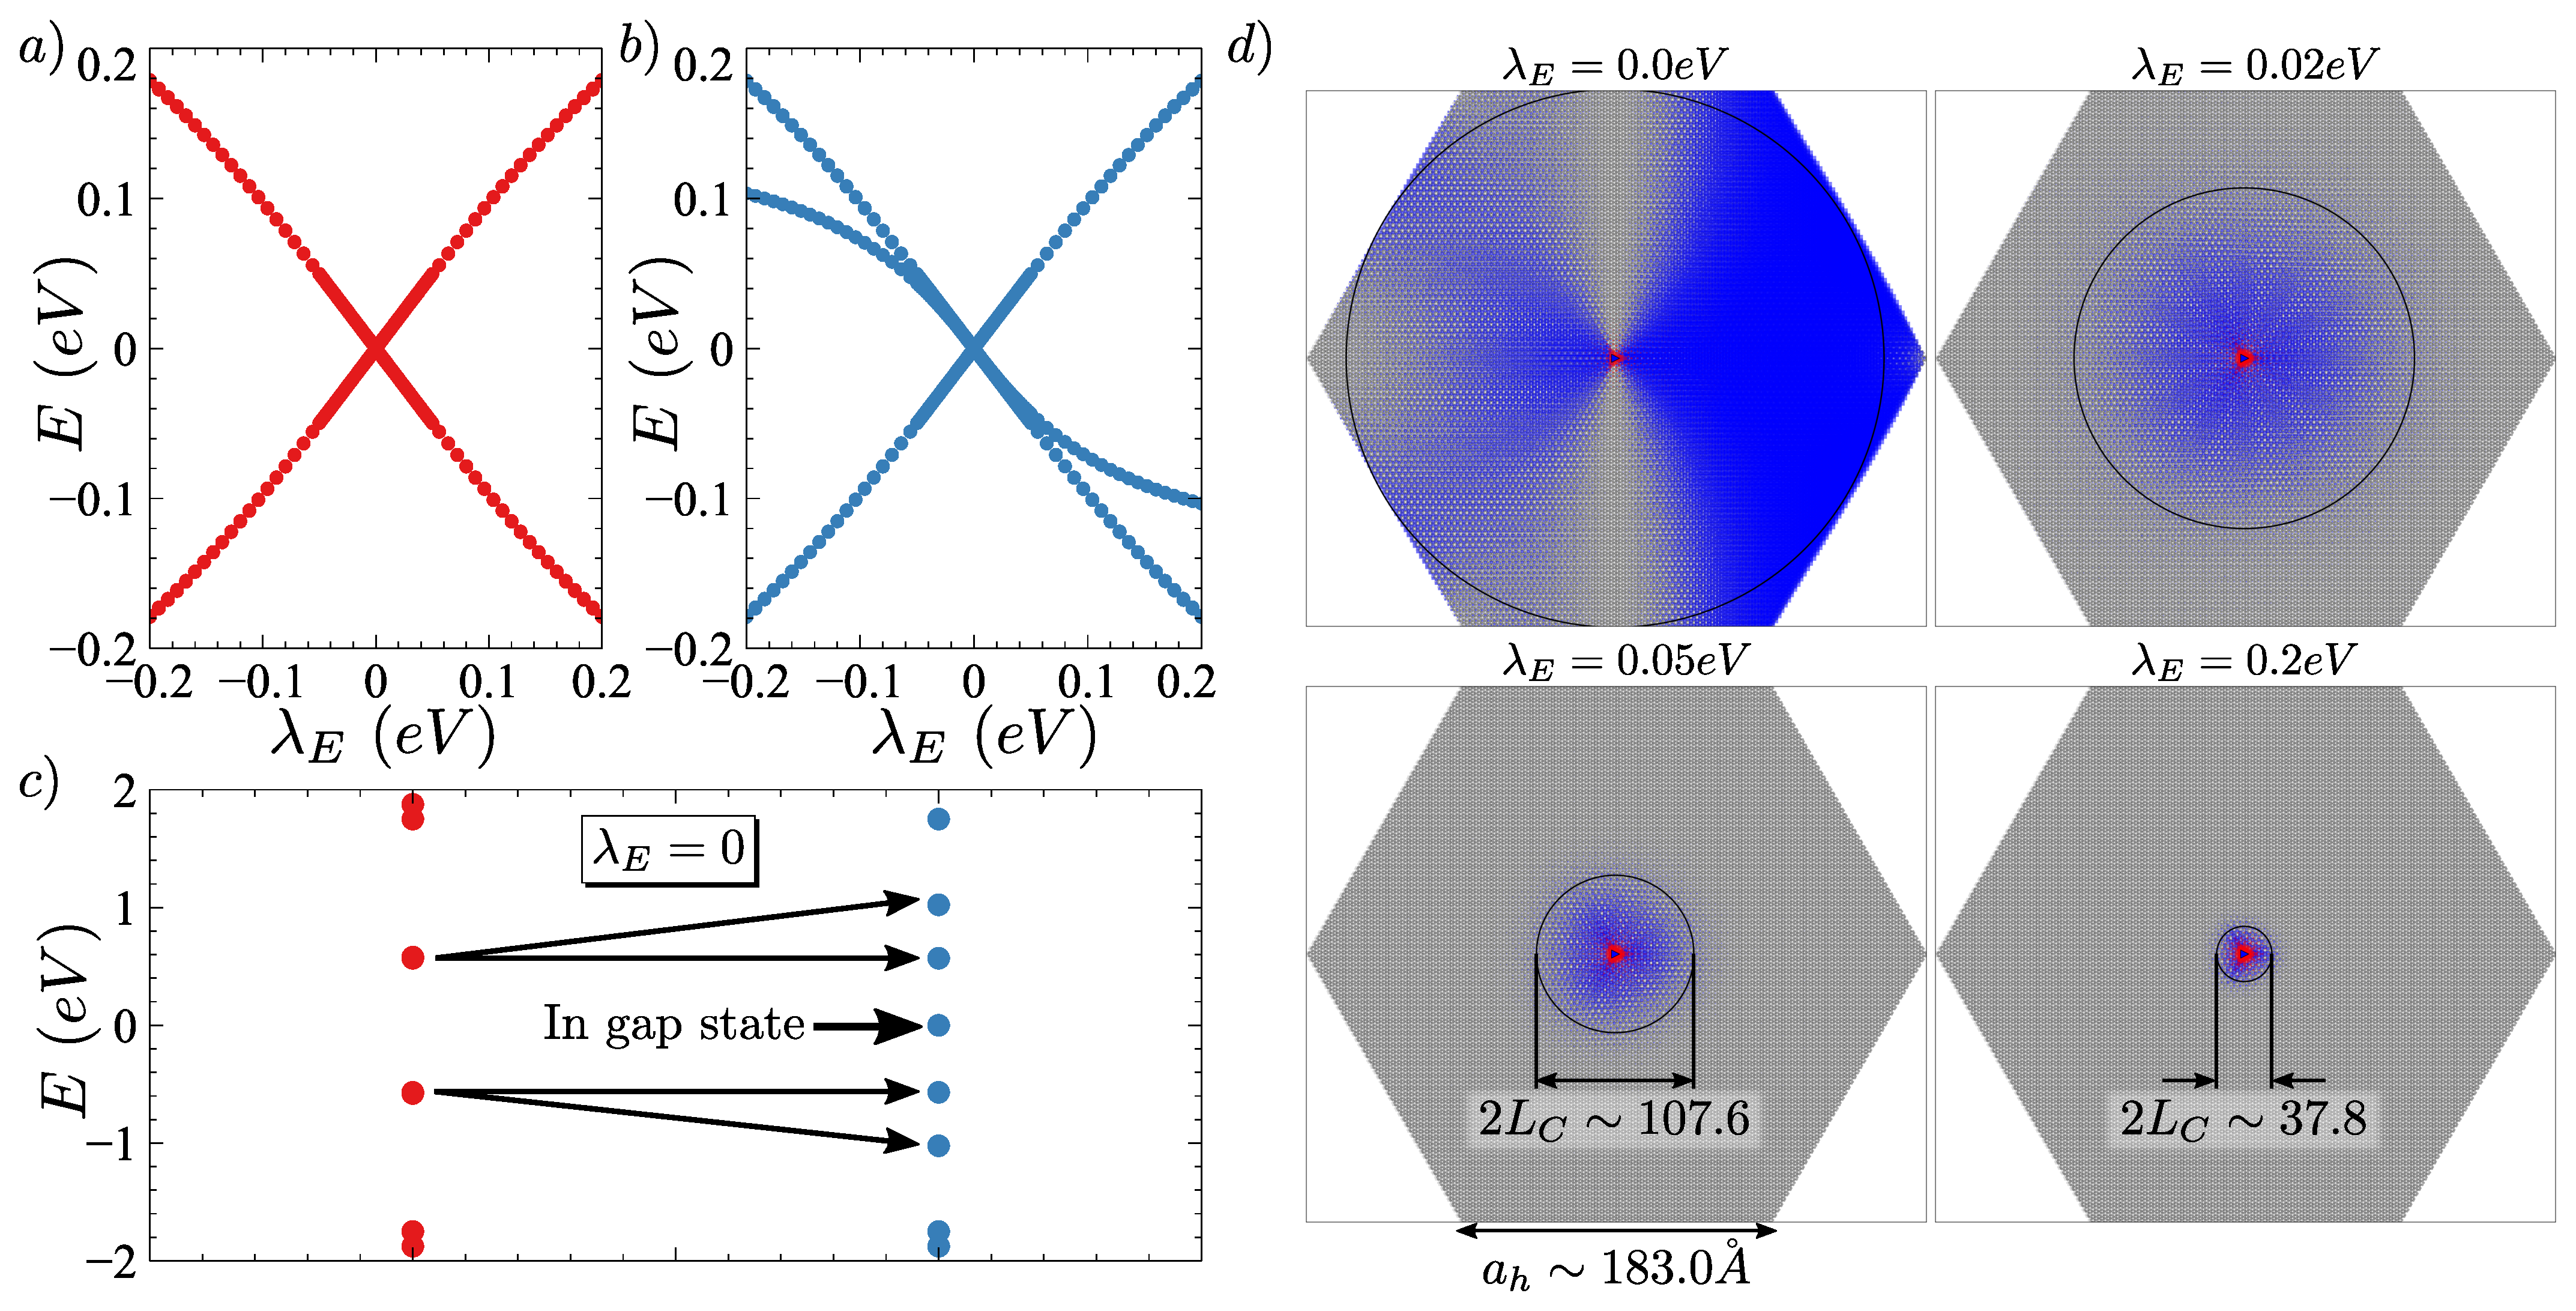
\includegraphics[width=\textwidth]{single_vac_spectrum.pdf}
% \vspace{-15pt}
% \caption{$a)$ and $b)$ show the pristine and defected spectrum respectively as a function of different applied electric fields. Notice the opening of a gap linear with the electric field (in both the pristine and defected cases) and the appearance of an extra state inside the gap. $c)$ Pristine (red) and defected (blue) spectrum for the case of no electric field $\lambda_E=0$. Panel $d)$ shows four snapshots of an island ($N_C=91812$ atoms) at different values of the electric field. The black circle in panel $d)$ shows the confinement length $L_C$ defined in the text.}
% \label{1vac_spec}
% \end{figure}
% \FloatBarrier
% %~~~~~~~~~~~~~~~~~~~~~~~~~~~~~~~~~~~~~~~~~~~~~~~~~~~~~~~~~~~%
%
% In Fig~\ref{1vac_spec} $d)$ we show four snapshots of the spatial distribution of the in-gap state. The actual lattice of the island is shown as black dots (probably indistinguishable because of the size of the image).
% On top of each atomic position the weight of the wave function ($|c_\beta|^2$ using the notation of eq.~\eqref{general}) is plotted in blue/red for the lower/upper layer.
% On top of all this, the site of the vacancy is marked with a blue triangle.
% As a visual guide the confinement length is plotted as a black circle with diameter $2L_C$.\\
%
% At $\lambda_E=0$ the system is bipartite, so according to the Lieb's theorem, after the removal of one site, a sublattice-polarized state should appear at $E=0$. This is exactly what happens as shown in Fig.~\ref{1vac_spec}.
%
% When we study the real-space distribution of the in-gap state we find that in the absence of electric field ($\lambda_E=0$) the state is spread all over the island, Fig.~\ref{1vac_spec} $d)$, no matter the size of the island (see Fig.~\ref{IPR_lc} $a)$ bellow). Notice that the effect of the border is not negligible in this regime and, in fact, is the responsible of the breaking of the expected $C_3$ symmetry of the state (at long distances, close to the vacancy the $C_3$ symmetry is almost preserved).
%
%
% Another important aspect is that the distribution of this wave function is such that in the upper layer (the one containing the vacancy) the wave function is quite confined around the vacancy (3-6 closest atoms) and it barely changes with the electric field, whereas in the lower layer the spreading of the wave function varies from the whole space available, to a few angstroms.
%
%
% To study quantitatively the properties of the in-gap state $\psi_0$ we define four quantities that will be useful later on.
% \begin{itemize}
%   \item \emph{Confinement length}, $L_C$, defined, hand-wavingly, as the distance at which more than $90\%$ of the state is located
%   \begin{equation}
%     0.9 = \int_{0}^{L_C} \psi_0(r) dr   %XXX arreglar!!!
%     \label{loclen}
%   \end{equation}
%   This confinement length can be used as a measurement of the spreading of the in-gap state $\psi_0$.
%   \begin{equation}
%     L'_C = \bra{\psi_0} |R-r_0|^2\ket{\psi_0}
%   \end{equation}
%   \item \emph{Inverse participation ratio} (IPR), $\eta$. Using the notation of equation~\eqref{general}, the IPR can be defined as:
%   \begin{equation}
%     \ket{\psi_0} = \sum_\beta c_\beta\ket{\phi_\beta}\quad\quad;\quad\quad
%     \text{IPR} = \eta = \sum_i |c_\beta|^4
%   \end{equation}
%   \item \emph{Sublattice} and \emph{Layer polarization}, defined as the expected value of the in-gap state.
%   \begin{equation}
%     SP = \bra{\psi_0}\widehat{\mathcal{S}}\ket{\psi_0}
%     \quad\quad;\quad\quad
%     SL = \bra{\psi_0}\widehat{\mathcal{L}}\ket{\psi_0}
%   \end{equation}
%   where the operators $\widehat{\mathcal{S}}$ and $\widehat{\mathcal{L}}$ measure the component of a given state in a given sublattice and layer respectively. Both $SP$ and $SL$ have to be, by definition, in the closed interval $\left[-1,1\right]$.
% \end{itemize}
%
% In figure~\ref{IPR_lc} we study the dependence of these four properties, for different sizes of the island, as a function of the electric field.
% %~~~~~~~~~~~~~~~~~~~~~~~~~~ FIGURE ~~~~~~~~~~~~~~~~~~~~~~~~~%
% \begin{figure}[!ht]
% \centering
% 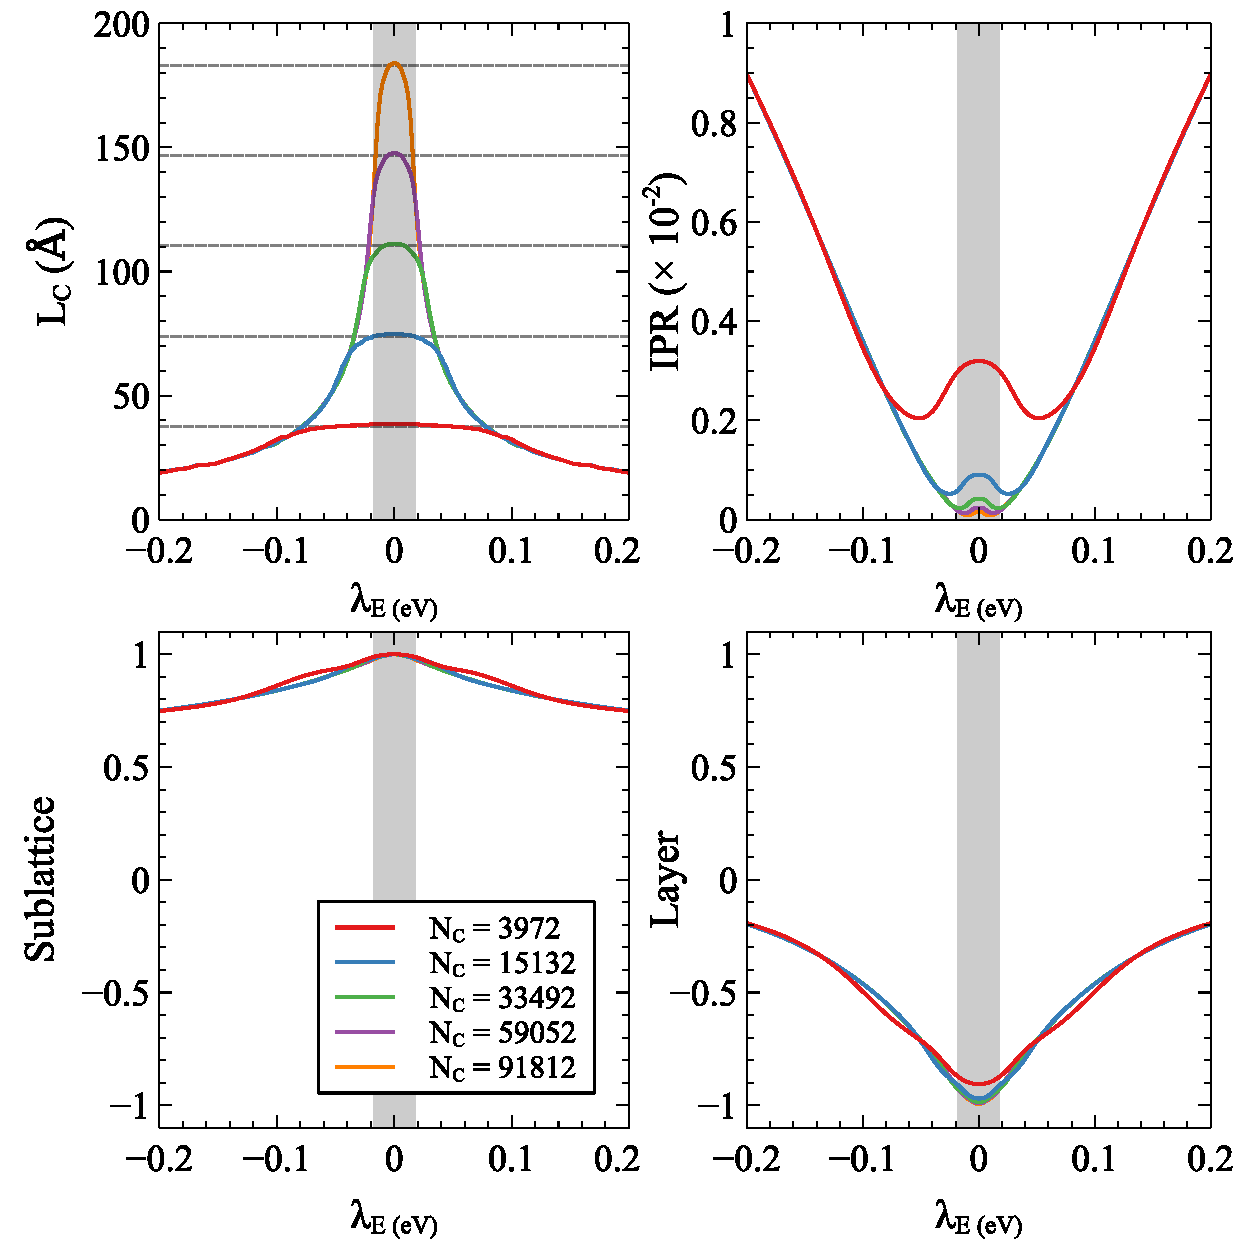
\includegraphics[width=0.6\textwidth]{single_vac_properties.pdf}
% \vspace{-5pt}
% \caption{$a)$ Dependence of the localization length $L_c$ with the electric field for different sizes of the island. The dashed lines corresponds to the size of the each corresponding island. $b)$ IPR, $\eta$, dependence with the electric field for different sizes of the island. $c)$ and $d)$ show the degree of sublattice and layer polarization for different sizes of the island as a function the electric field. The values $\pm1$ refer to $A/B$ sublattice or up/down layer respectively.}
% \label{IPR_lc}
% \end{figure}
% \FloatBarrier
% %~~~~~~~~~~~~~~~~~~~~~~~~~~~~~~~~~~~~~~~~~~~~~~~~~~~~~~~~~~~%
%
% It can be seen in Fig.~\ref{IPR_lc} $a)$ that as we approach the limit $\lambda_E\rightarrow0$ the confinement length collapses to the size of the island, shown as a dashed line for each size studied. This plateau is just the effect of having an in-gap state spread all over the island.
%
% The shadowed region in all the panels shows the range of $\lambda_E$ in which the border effects can be relevant for the biggest island studied ($N_C=91812$). It is estimated as the $\lambda_E$ at which the results differ from those of the previous island. Of course it is only a rough estimation and it should be considered only as a guide to the eye when reading the results.
%
% In panel $b)$ the IPR is shown. Except for small islands the evolution of the IPR, as that of the $L_C$, is the same regardless of the size of the island. The increasing of the IPR with the electric field is another sign of the increasing localization of the in-gap state around the vacancie.\\
%
% The sublattice and layer polarization are shown in panels~\ref{IPR_lc} $c)$ and $d)$. As it can be seen at $\lambda_E=0$ the state is completely sublattice-polarized, in accordance with the Lieb's theorem, and almost layer-polarized, this almost is more easly visible in the small red component present in Fig.~\ref{1vac_spec} $d)$.
%
% As the electric field increases the bipartite character of the system is lost, in agreement with the shift of the energy of the in-gap state (no longer at $E=0$). Since the system is no longer bipartite, the sublattice polarized character of the in-gap state is no longer assured, and as shown in panel $c)$ it, in fact, decreases.
%
% The decreasing of the layer polarization is easily understood by looking at Fig.~\ref{1vac_spec} $d)$. For small $\lambda_E$ the in-gap state is mostly spread over the lower layer, while for large $\lambda_E$ the in-gap state occupies roughly the same area in both layers resulting in a $\bra{\psi_0}\widehat{\mathcal{L}}\ket{\psi_0} \rightarrow 0$
%
%
%
%
% % When a single $p_z$ site is removed from graphene, an electron is confined in the surroundings of the vacancy with energy $E=0$. While it is true that such a state is mainly localized in the 3 closest neighbors, the rest of the state is diluted in all the other available sites. \red{[non-renormalizable?]}
% %
% % Interestingly, when a gap is open, the state becomes normalizable and a confinement length can be defined. In particular, the confinement length is controlled by the size of the gap.
% %
% % Graphene bilayer shows a tuneable band gap when an external electric field is applied\cite{}. This manipulation of the gap provides an excellent tool to control the confinement of any in-gap state.
% %
% % We will use an island of graphene bilayer with 91812 atoms. The removal of the hollow site closest to the center of the island results in an in-gap state as shown in Fig~\ref{single_vac}.
% %
% % %~~~~~~~~~~~~~~~~~~~~~~~~~~ FIGURE ~~~~~~~~~~~~~~~~~~~~~~~~~%
% % \begin{figure}[h!]
% % \centering
% %   \includegraphics[width=0.7\textwidth]{single_vacancy.pdf}
% % \vspace{-5pt}
% % \caption{Effect of an external electric field in the ingap state of a graphene bilayer with a single vacancy \red{include bands}}
% % \label{single_vac}
% % \end{figure}
% % \FloatBarrier
% % %~~~~~~~~~~~~~~~~~~~~~~~~~~~~~~~~~~~~~~~~~~~~~~~~~~~~~~~~~~~%

%~~~~~~~~~~~~~~~~~~~~~~~~~~ FIGURE ~~~~~~~~~~~~~~~~~~~~~~~~~%
\begin{figure}[h!]
\centering
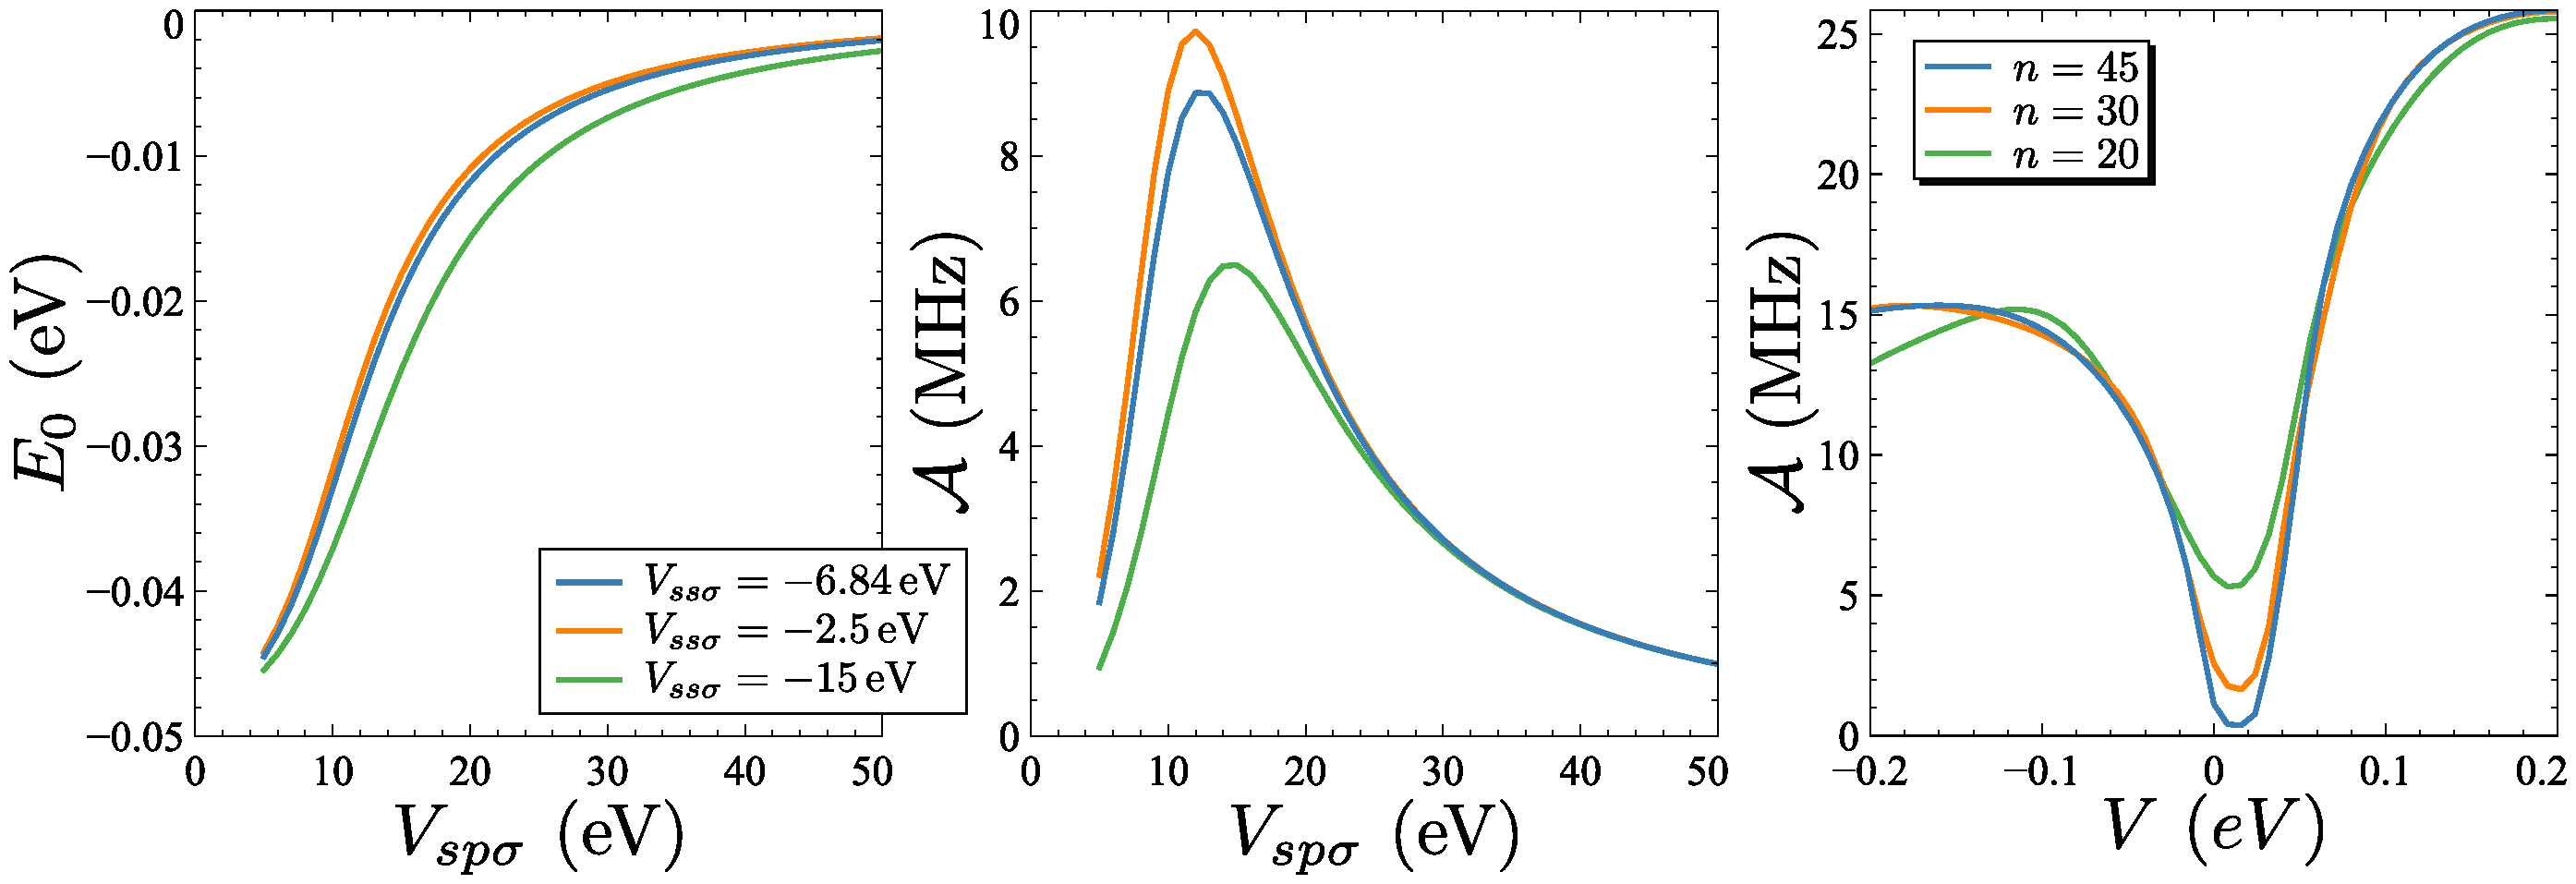
\includegraphics[width=\textwidth]{artlat/fig/hyperfine.pdf}
\vspace{-20pt}
\caption{Change in the hyperfine coupling with the electric field.}
\label{Label}
\end{figure}
\FloatBarrier
%~~~~~~~~~~~~~~~~~~~~~~~~~~~~~~~~~~~~~~~~~~~~~~~~~~~~~~~~~~~%



\section{2-D. Designer fermion lattices} %~~~~~~~~~~~~~~~~~~~~~~~~~~~~~~~~~~~~~%
By carefully choosing the placement of the vacancies, different 2D lattices can be designed. The electrically tunable gap as well as the distance among vacancies provide two parameters to design fermion models with the desired parameters.
Almost any lattice is feasible, as illustrative examples we will examine a triangular lattice with different unit cells, i.e., a simple triangular lattice, graphene and the Kagome lattice.

The effective parameters will be tuned by choosing the appropriate distances and angles between vacancies and the corresponding electric field.


\subsection{Artificial triangular lattice}
The simplest effective lattice that can be designed is a triangular lattice with a single site per unit cell. This lattice appears naturally when we consider only the hollow positions of the upper layer in a graphene bilayer.

%~~~~~~~~~~~~~~~~~~~~~~~~~~ FIGURE ~~~~~~~~~~~~~~~~~~~~~~~~~%
\begin{figure}[h!]
  \centering
  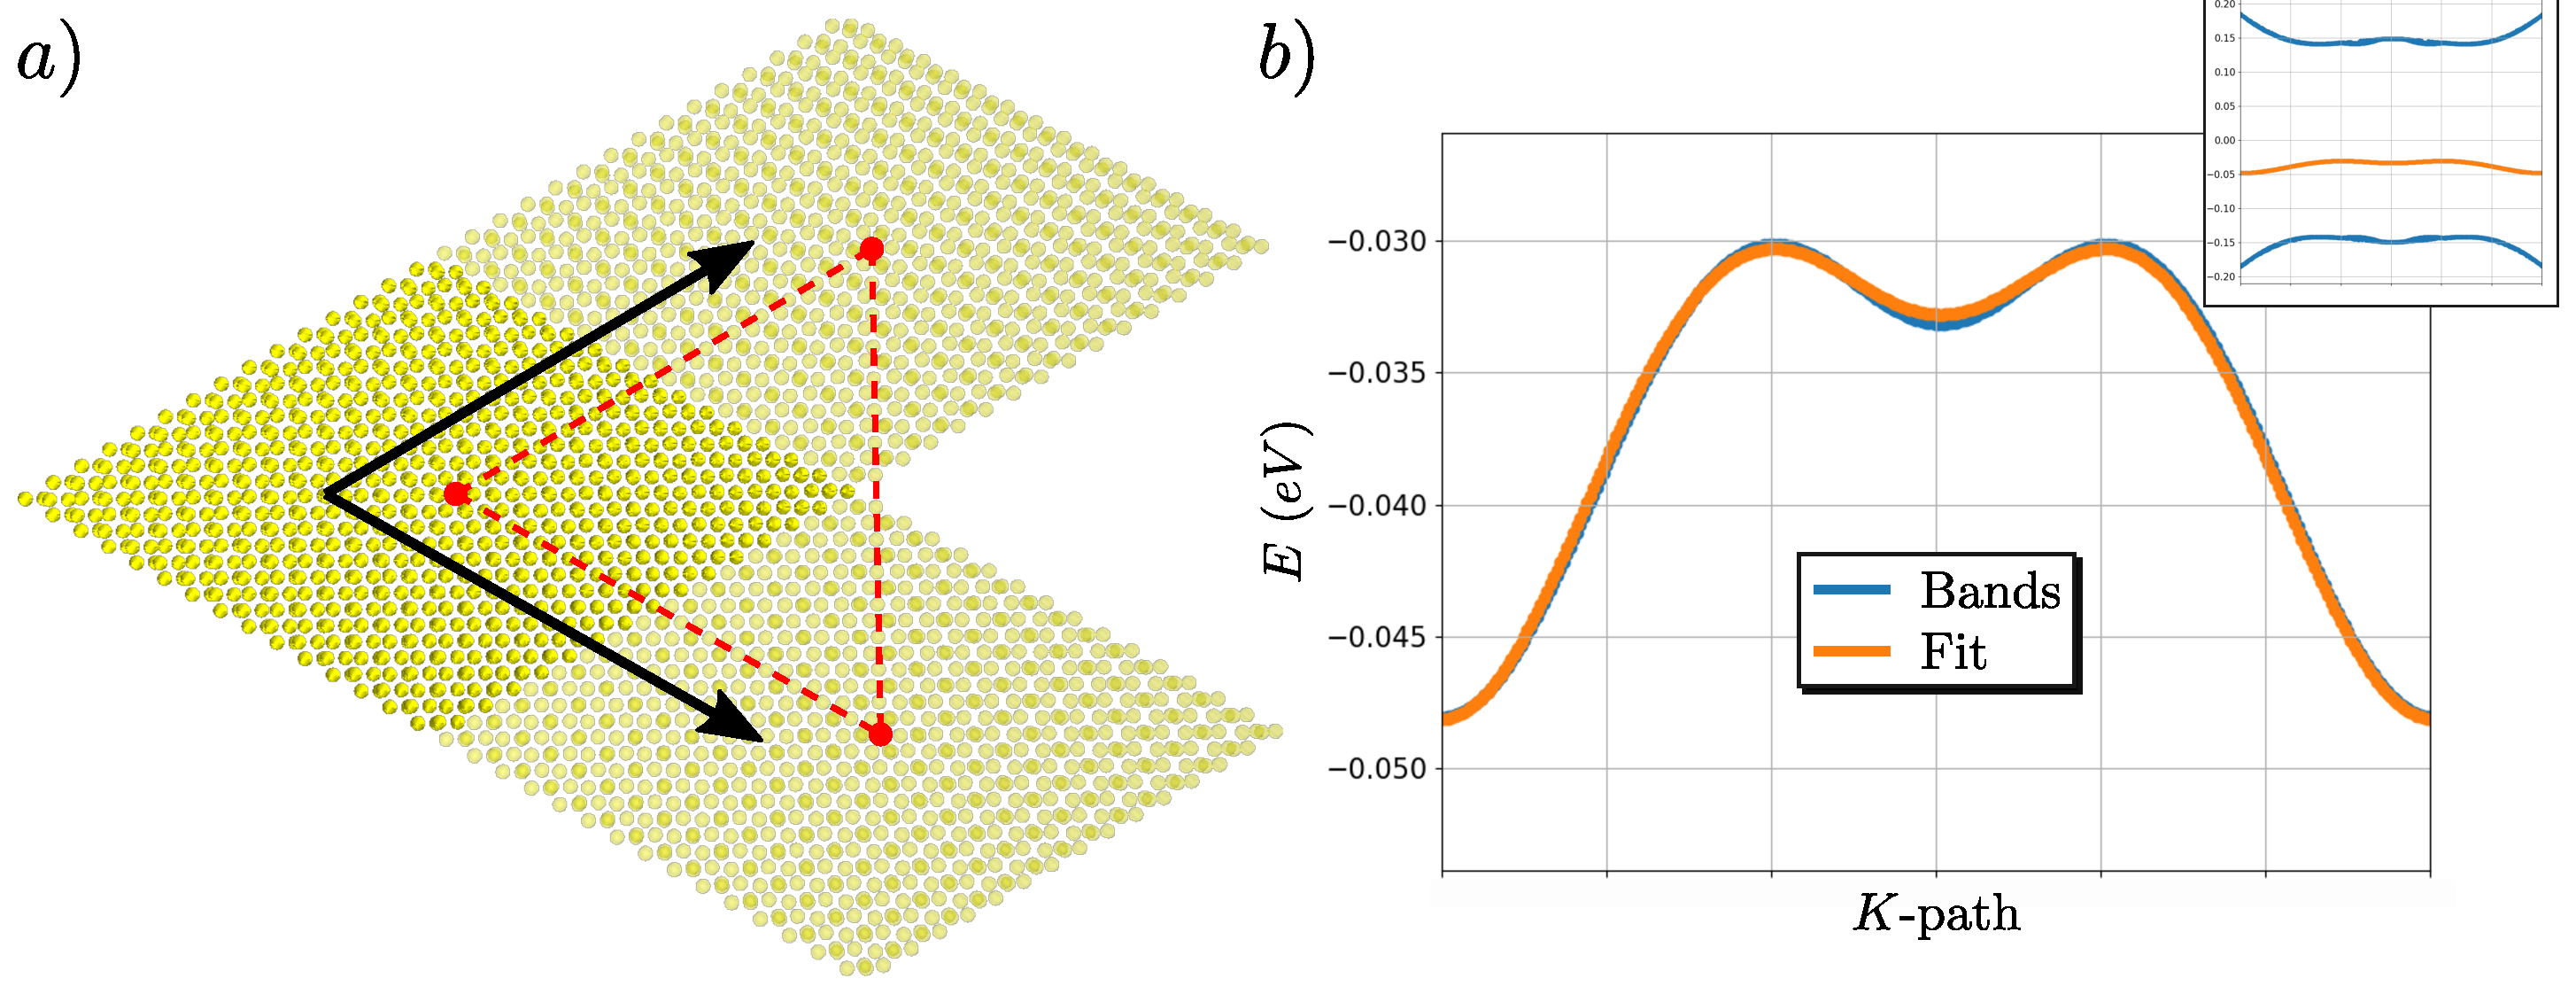
\includegraphics[width=0.8\textwidth]{artlat/fig/triangular_bands.pdf}
  \vspace{-5pt}
  \caption{$a)$ shows an example of a unit cell with the vacancies placed in such a way that the translational symmetry creates an artificial triangular lattice. $b)$ shows the in-gap bands (orange in the inset) that appear because of the vacancies, the fit is done using a model with up to third neighbors.}
  \label{triangular}
\end{figure}
\FloatBarrier
%~~~~~~~~~~~~~~~~~~~~~~~~~~~~~~~~~~~~~~~~~~~~~~~~~~~~~~~~~~~%

In Fig.~\ref{triangular} $a)$ we can be the architecture considered, a single vacancy in the center of the unit cell and the standard lattice vectors for a graphene supercell. The lattice of impurities form an in-gap band which resembles that of a triangular lattice.
In particular it can be fit to a model like:
\begin{equation}
\begin{split}
  H(k) = E_0 &+
         2t_1\left[ cos\left(\vec{k}\vec{a}_1\right) +
                    cos\left(\vec{k}\vec{a}_2\right) +
                    cos\left(\vec{k}(\vec{a}_1-\vec{a}_2)\right)
              \right] +\\
         &+2t_2\left[ cos\left(\vec{k}(\vec{a}_1+\vec{a}_2)\right) +
                    cos\left(\vec{k}(2\vec{a}_1-\vec{a}_2)\right) +
                    cos\left(\vec{k}(-\vec{a}_1+2\vec{a}_2)\right)
             \right] +\\
         &+2t_3\left[ cos\left(2\vec{k}\vec{a}_1\right) +
                    cos\left(2\vec{k}\vec{a}_2\right) +
                    cos\left(2\vec{k}(\vec{a}_1-\vec{a}_2)\right)
              \right]
\end{split}
\label{triangular_hamil}
\end{equation}
Where $\vec{k}$, $\vec{a}_1$ and $\vec{a}_2$ are the Bloch vector and the lattice vectors respectively. The parameters that best fit the model \eqref{triangular_hamil} are the following:
\begin{equation}
\begin{split}
  E_0 &= \SI{-0.036}{\eV}\\
  t_1 = \SI{-1.93e-3}{\eV} \quad;\quad
  t_2 &= \SI{7.40e-5}{\eV} \quad;\quad
  t_3 = \SI{-5.26e-5}{\eV}
\end{split}
\end{equation}


\subsection{Artificial graphene}
In order to create an artificial graphene crystal we need to place the vacancies at a particular distance that depends on the size of the chosen unit cell.
The basic unit cell and lattice vectors for graphene are
\begin{equation}
\begin{split}
  r_0 = a\left(-\frac{1}{2},0,0\right) \qquad ; \qquad
  r_1 = a\left(\frac{1}{2},0,0\right)\\
  a_1 = a\left(\frac{3}{2},\frac{\sqrt{3}}{2},0\right) \qquad ; \qquad
  a_2 = a\left(\frac{3}{2},-\frac{\sqrt{3}}{2},0\right)
\end{split}
\end{equation}
In order to separate the vacancies, bigger cells must be used, the lattice vectors will escalate for a cell of size $n$:
\begin{equation}
  \vec{a}^n_1 = n \vec{a}_1 \qquad ; \qquad \vec{a}^n_2 = n \vec{a}_2
\end{equation}
Since the vacancies have to be in the same sublattice, the possible distances for them are $d_v = 3na$, being $a=\SI{1.4}{\angstrom}$ the $C$-$C$ distance. The corresponding lattice vectors should be:
\begin{equation}
  \vec{a}^n_1 = 3na\left(\frac{3}{2},\frac{\sqrt{3}}{2},0\right) \qquad ; \qquad
  \vec{a}^n_2 = 3na\left(\frac{3}{2},-\frac{\sqrt{3}}{2},0\right)
\end{equation}
This simple relation shows that only supercells which are a multiple of 3 are feasible.


% Therefore a perfect graphene lattice will only emerge when $|\vec{a}^n_1|=|\vec{a}^n_2|=3na$. Notice that $m$ and $n$ are independent indices.
% \begin{equation}
%   |\vec{a}^n| = \sqrt{3}na \quad\Rightarrow n = \sqrt{3}m
% \end{equation}
% \red{Impossible?!}

When the vacancies are placed at that distance, and are properly oriented (see Fig~\ref{graphene}) the in-gap states interact among them forming two dispersing bands all over the Brillouin zone.
%~~~~~~~~~~~~~~~~~~~~~~~~~~ FIGURE ~~~~~~~~~~~~~~~~~~~~~~~~~%
\begin{figure}[h!]
  \centering
  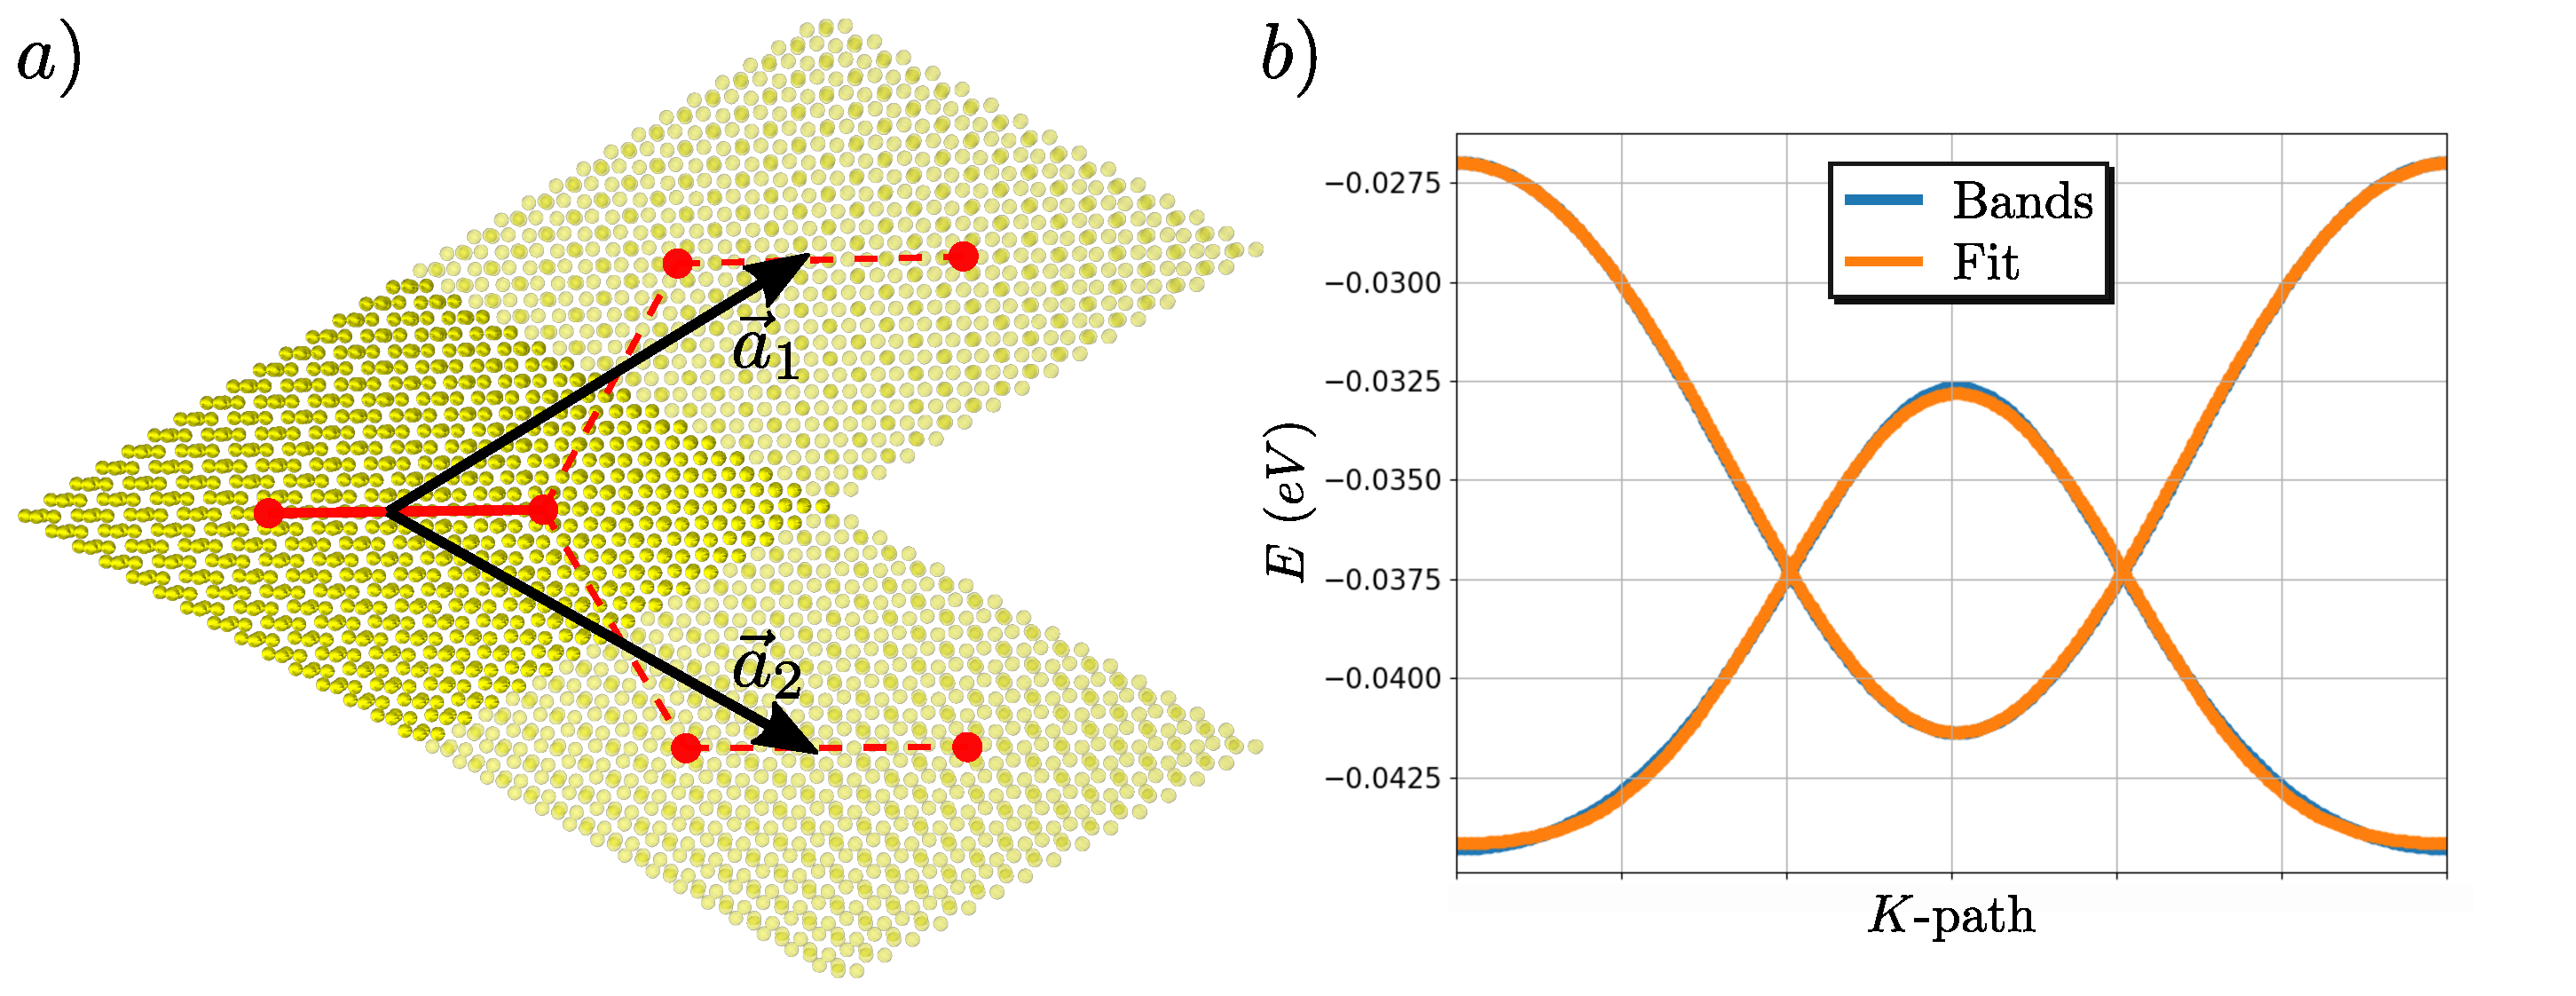
\includegraphics[width=0.8\textwidth]{artlat/fig/graphene_bands.pdf}
  \vspace{-5pt}
  \caption{$a)$ shows an example of a unit cell with the vacancies placed in such a way that the translational symmetry creates an artificial graphene lattice. $b)$ shows the in-gap bands (orange) that appear because of the vacancies, the fit is done using a model with up to third neighbors.}
  \label{graphene}
\end{figure}
\FloatBarrier
%~~~~~~~~~~~~~~~~~~~~~~~~~~~~~~~~~~~~~~~~~~~~~~~~~~~~~~~~~~~%
In Fig.~\ref{graphene} $b)$ we can see the dispersing in-gap bands as well as a fit of said bands to a simple model with up to third neighbors.

\begin{equation}
\begin{split}
  % E_0 = \SI{-0.03670772697798405}{\eV}
  % t_1 = \SI{-0.003216525825060562}{\eV}
  % t_2 = \SI{0.00018838793316003813}{\eV}
  % t_3 = \SI{0.0003533798537212944}{\eV}
  E_0 &= \SI{-0.037}{\eV}\\
  t_1 = \SI{-3.22e-3}{\eV} \quad;\quad
  t_2 &= \SI{1.88e-4}{\eV} \quad;\quad
  t_3 = \SI{3.53e-4}{\eV}
\end{split}
\end{equation}

%~~~~~~~~~~~~~~~~~~~~~~~~~~ FIGURE ~~~~~~~~~~~~~~~~~~~~~~~~~%
\begin{figure}[!ht!]
\centering
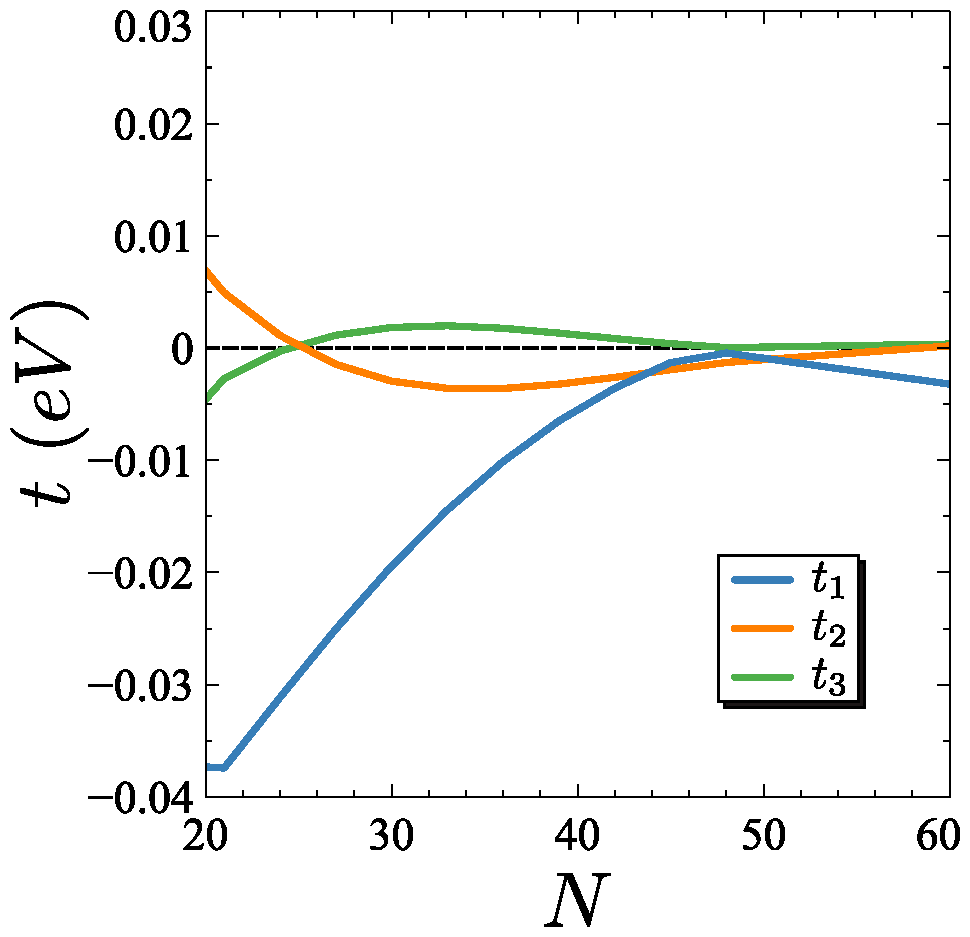
\includegraphics[width=0.5\textwidth]{artlat/fig/params.pdf}
\vspace{-5pt}
\caption{Evolution of the hopping parameters of a graphene tight-binding model with third neighbor hoppings.}
\label{hopp}
\end{figure}
\FloatBarrier
%~~~~~~~~~~~~~~~~~~~~~~~~~~~~~~~~~~~~~~~~~~~~~~~~~~~~~~~~~~~%






\subsection{Artificial Kagome}
the position of the adatoms to have an artificial Kagome lattice are:
\begin{equation}
  r_1 = \frac{a_k}{2}\left(\sqrt{3}/2,  0 ,0\right),\quad
  r_2 = \frac{a_k}{2}\left(-\sqrt{3}/2,1,0\right),\quad
  r_3 = \frac{a_k}{2}\left(-\sqrt{3}/2,-1,0\right)
\end{equation}

where $a_k = |a_1|/2$. This geometry only works regularly for odd supercells as seeing in Fig.~\ref{kagome}


%~~~~~~~~~~~~~~~~~~~~~~~~~~ FIGURE ~~~~~~~~~~~~~~~~~~~~~~~~~%
\begin{figure}[h!]
  \centering
  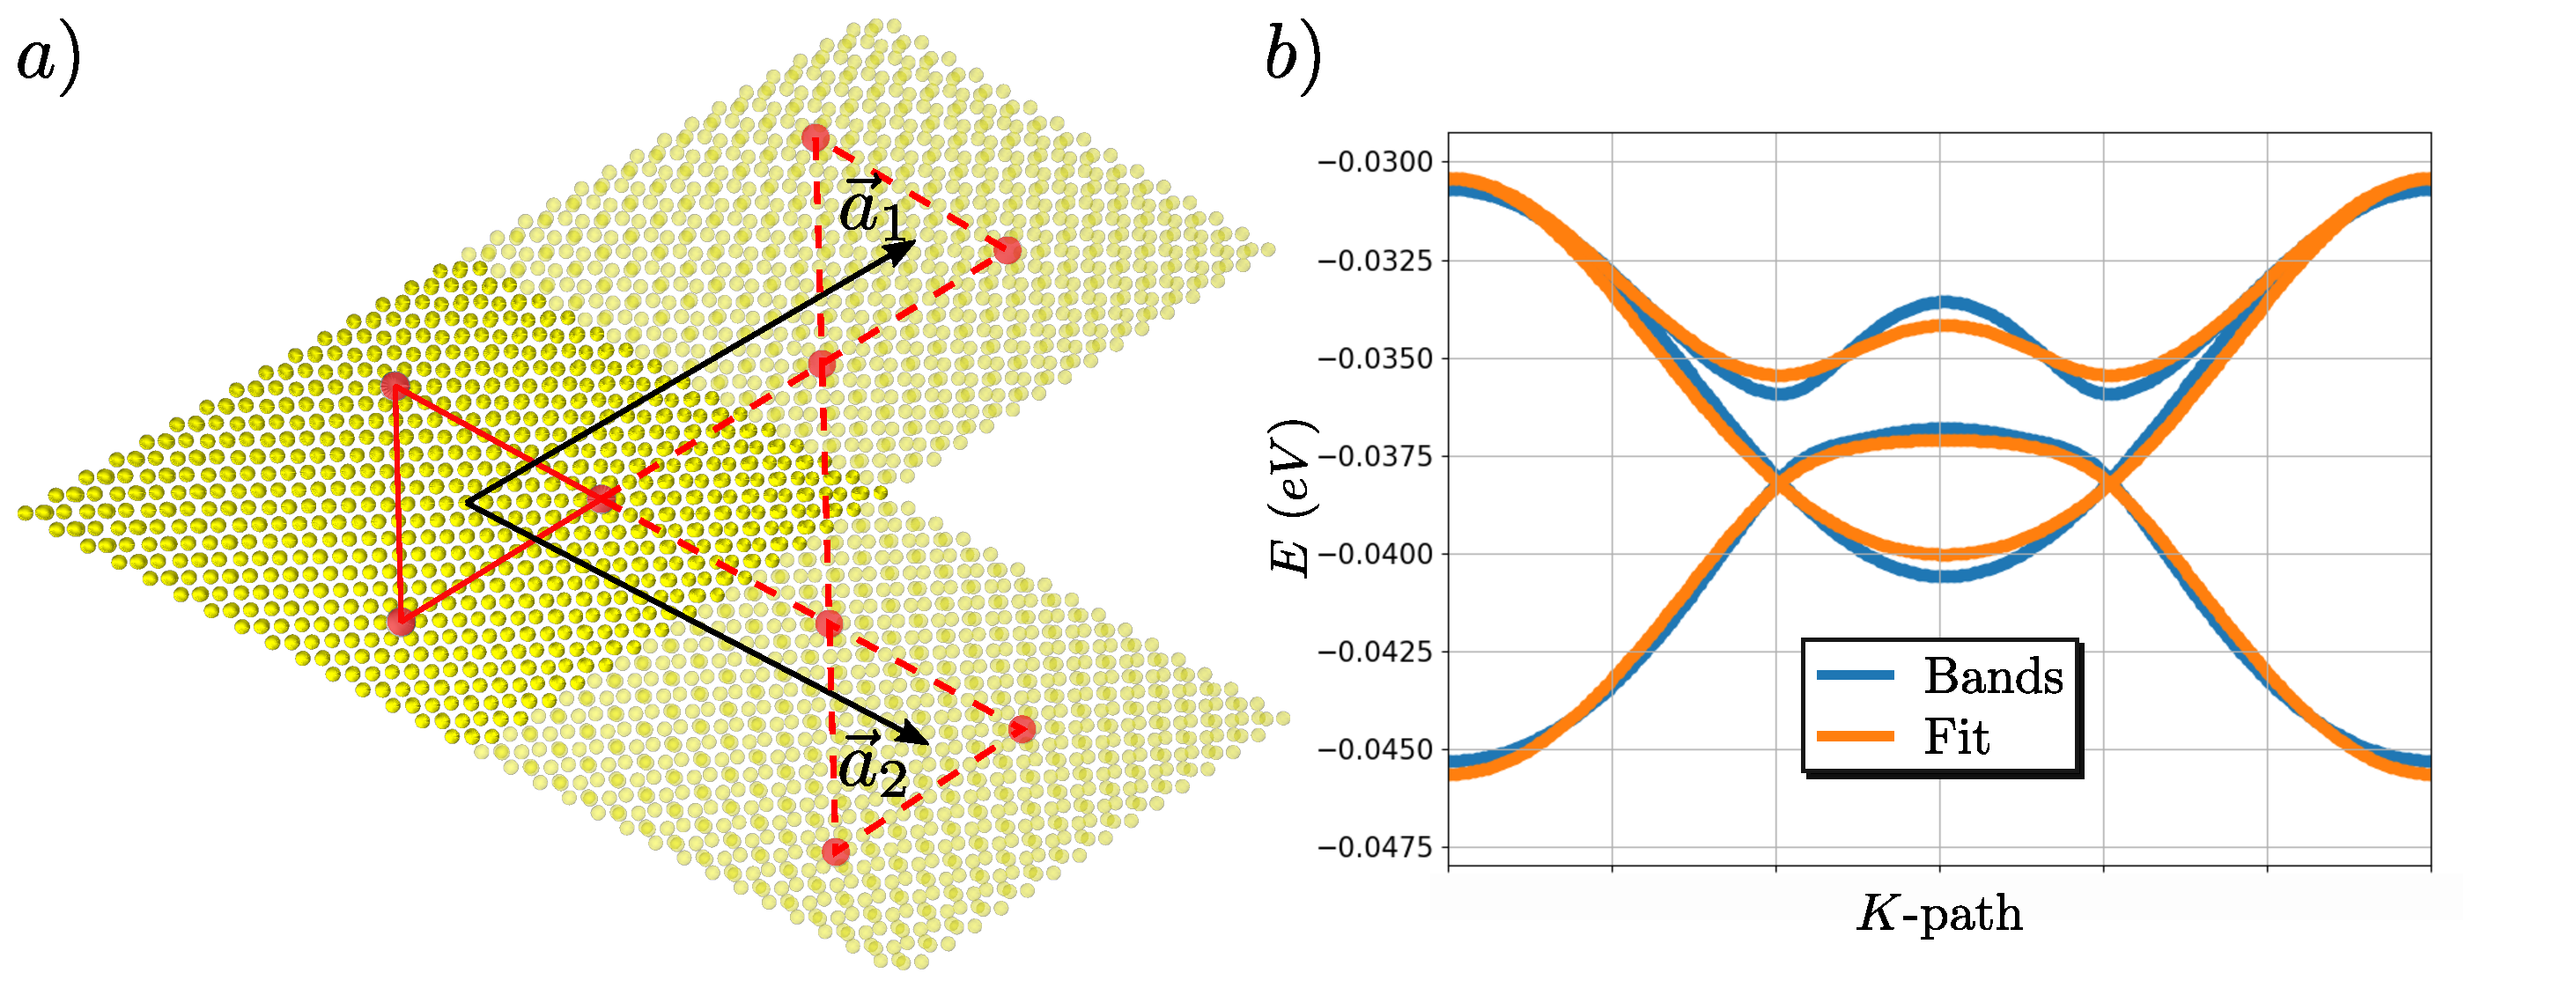
\includegraphics[width=0.8\textwidth]{artlat/fig/kagome_bands.pdf}
  \vspace{-5pt}
  \caption{$a)$ shows an example of a unit cell with the vacancies placed in such a way that the translational symmetry creates an artificial Kagome lattice. $b)$ shows the in-gap bands (orange) that appear because of the vacancies, the fit is done using a model with up to second neighbors.}
  \label{kagome}
\end{figure}
\FloatBarrier
%~~~~~~~~~~~~~~~~~~~~~~~~~~~~~~~~~~~~~~~~~~~~~~~~~~~~~~~~~~~%
\begin{equation}
\begin{split}
  % E_0 = -0.03669201703555982
  % t_1 = -0.002000033597883536
  % t_2 = -0.000536649553068988
  % t_3 = 0.00020143407845221853
  E_0 &= \SI{-0.037}{\eV}\\
  t_1 = \SI{-2.00e-3}{\eV} \quad;\quad
  t_2 &= \SI{-5.37e-4}{\eV} \quad;\quad
  t_3 = \SI{2.01e-4}{\eV}
\end{split}
\end{equation}
A geometric cheat sheet can be found in appendix~\ref{models}





\section{Parameters control. Hubbard dimer}

In order to determine the ground state as a function of both the electric field $\mathcal{E}$ and the distance between vacancies $d$ we use the fact that the spectrum of the blue Hamiltonian looks like one of the structures shown in Fig.~\ref{spectrum_dimer}. Considering the standard deviation of the 3 lowest eigenvalues (0-2), and the same quantity skipping one eigenvalue (1-3) we can obtain a quantity that will flip sign if the singlet and triplet cross.

%~~~~~~~~~~~~~~~~~~~~~~~~~~ FIGURE ~~~~~~~~~~~~~~~~~~~~~~~~~%
\begin{figure}[h!]
\centering
  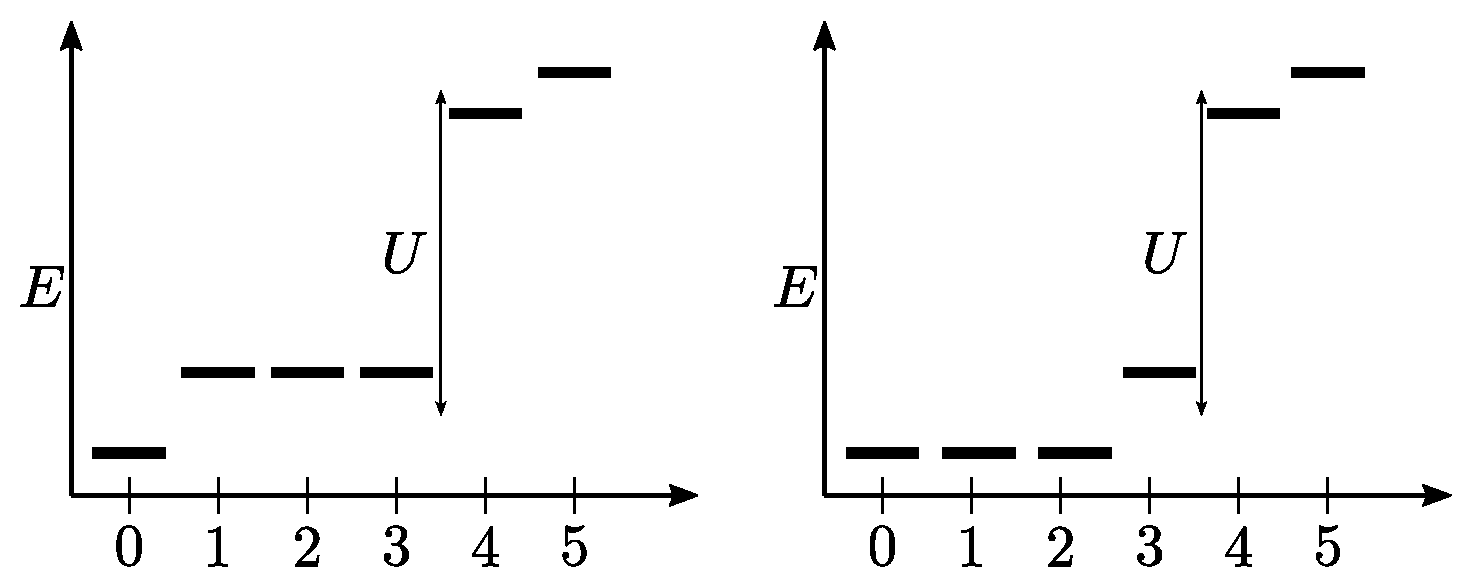
\includegraphics[width=0.7\textwidth]{artlat/fig/sketch_levels.pdf}
\vspace{-5pt}
\caption{Possible structure of the spectrum of the eigenvalues of the blue Hamiltonian.}
\label{spectrum_dimer}
\end{figure}
\FloatBarrier
%~~~~~~~~~~~~~~~~~~~~~~~~~~~~~~~~~~~~~~~~~~~~~~~~~~~~~~~~~~~%

%~~~~~~~~~~~~~~~~~~~~~~~~~~ FIGURE ~~~~~~~~~~~~~~~~~~~~~~~~~%
\begin{figure}[h!]
\centering
  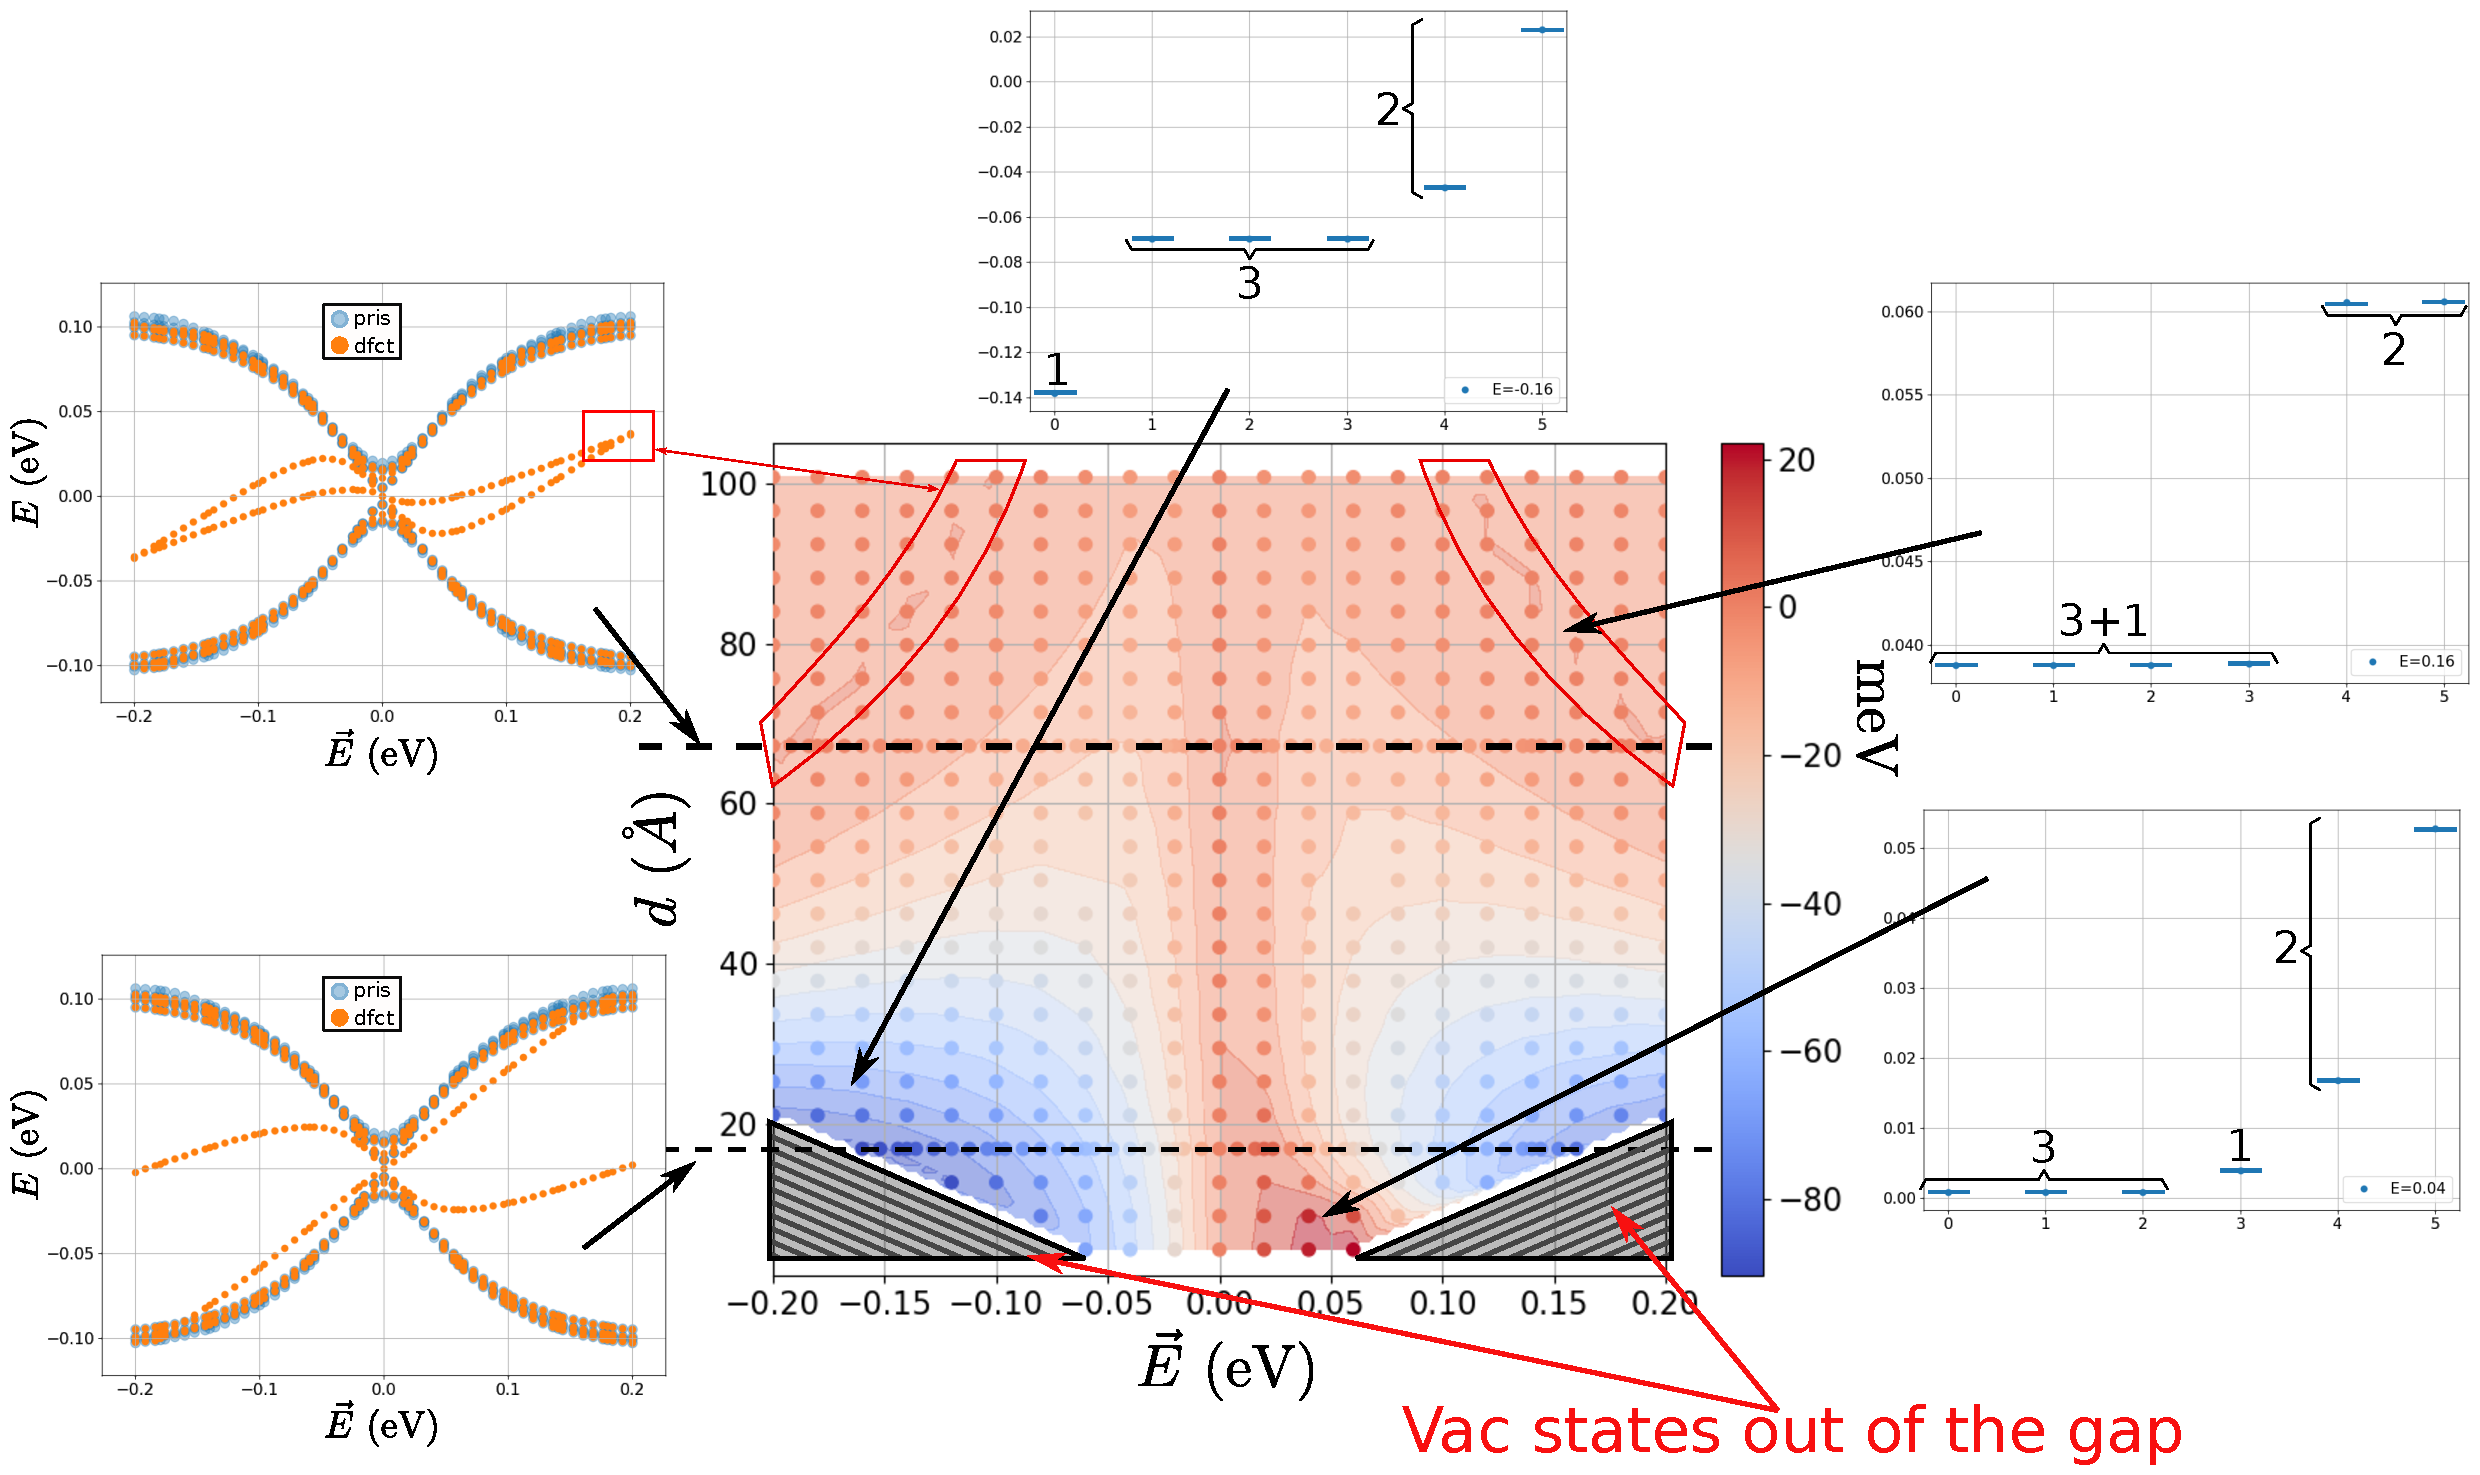
\includegraphics[width=0.7\textwidth]{artlat/fig/phase_J.pdf}
\vspace{-5pt}
\caption{Phase space showing the arrangement of the ground state as exposed in the text}
\label{}
\end{figure}
\FloatBarrier
%~~~~~~~~~~~~~~~~~~~~~~~~~~~~~~~~~~~~~~~~~~~~~~~~~~~~~~~~~~~%

%~~~~~~~~~~~~~~~~~~~~~~~~~~ FIGURE ~~~~~~~~~~~~~~~~~~~~~~~~~%
\begin{figure}[h!]
\centering
  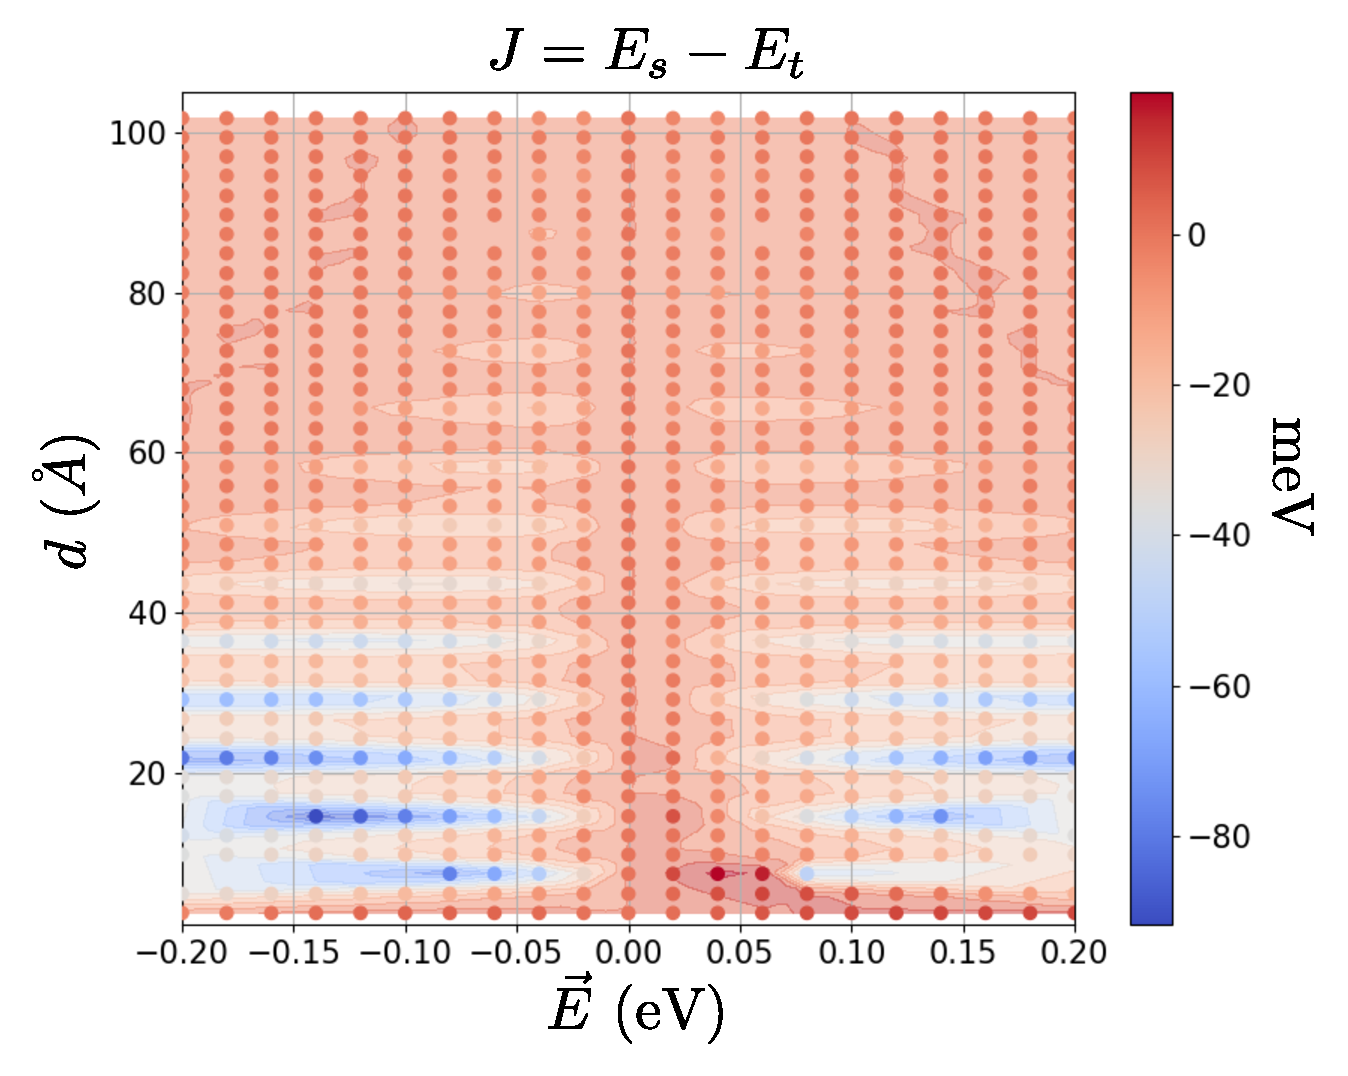
\includegraphics[width=0.7\textwidth]{artlat/fig/phase_J30.pdf}
\vspace{-5pt}
\caption{Phase space showing the arrangement of the ground state as exposed in the text for $\alpha=30$}
\label{}
\end{figure}
\FloatBarrier
%~~~~~~~~~~~~~~~~~~~~~~~~~~~~~~~~~~~~~~~~~~~~~~~~~~~~~~~~~~~%



%%~~~~~~~~ Chapter ~~~~~~~~
%% Graphene Bilayer
%\chapter{Graphene Bilayer}
\label{ch:bilayer}
Graphite is made out of two weakly bounded graphene layers. Extensive work has been devoted to systems in which two layers are isolated\cite{McCann2012}.

There are two ways to stack two graphene layers in a commensurate way. The first option is to align directly one layer on top of the other, so every atom in one layer is connected to an atom from the other layer. This is the so-called $AA$-stacking.
The other option is to have the top layer shifted by one atomic position as shown in \fref{Gbi_stack}c). The later stacking, commonly called Bernal stacking or $AB$-stacking, is the most common one according to both experiments and \ac{dft} calculations\cite{Norimatsu2010,Charlier1994,Charlier1994a}.

In both stackings the overall band structure (see \fref{Gbi_stack}b,d)) is quite similar since the interlayer interaction is around one order of magnitude weaker than any intralayer hopping.
%~~~~~~~~~~~~~~~~~~~~~~~~~~ FIGURE ~~~~~~~~~~~~~~~~~~~~~~~~~%
\begin{figure}[h!]
\centering
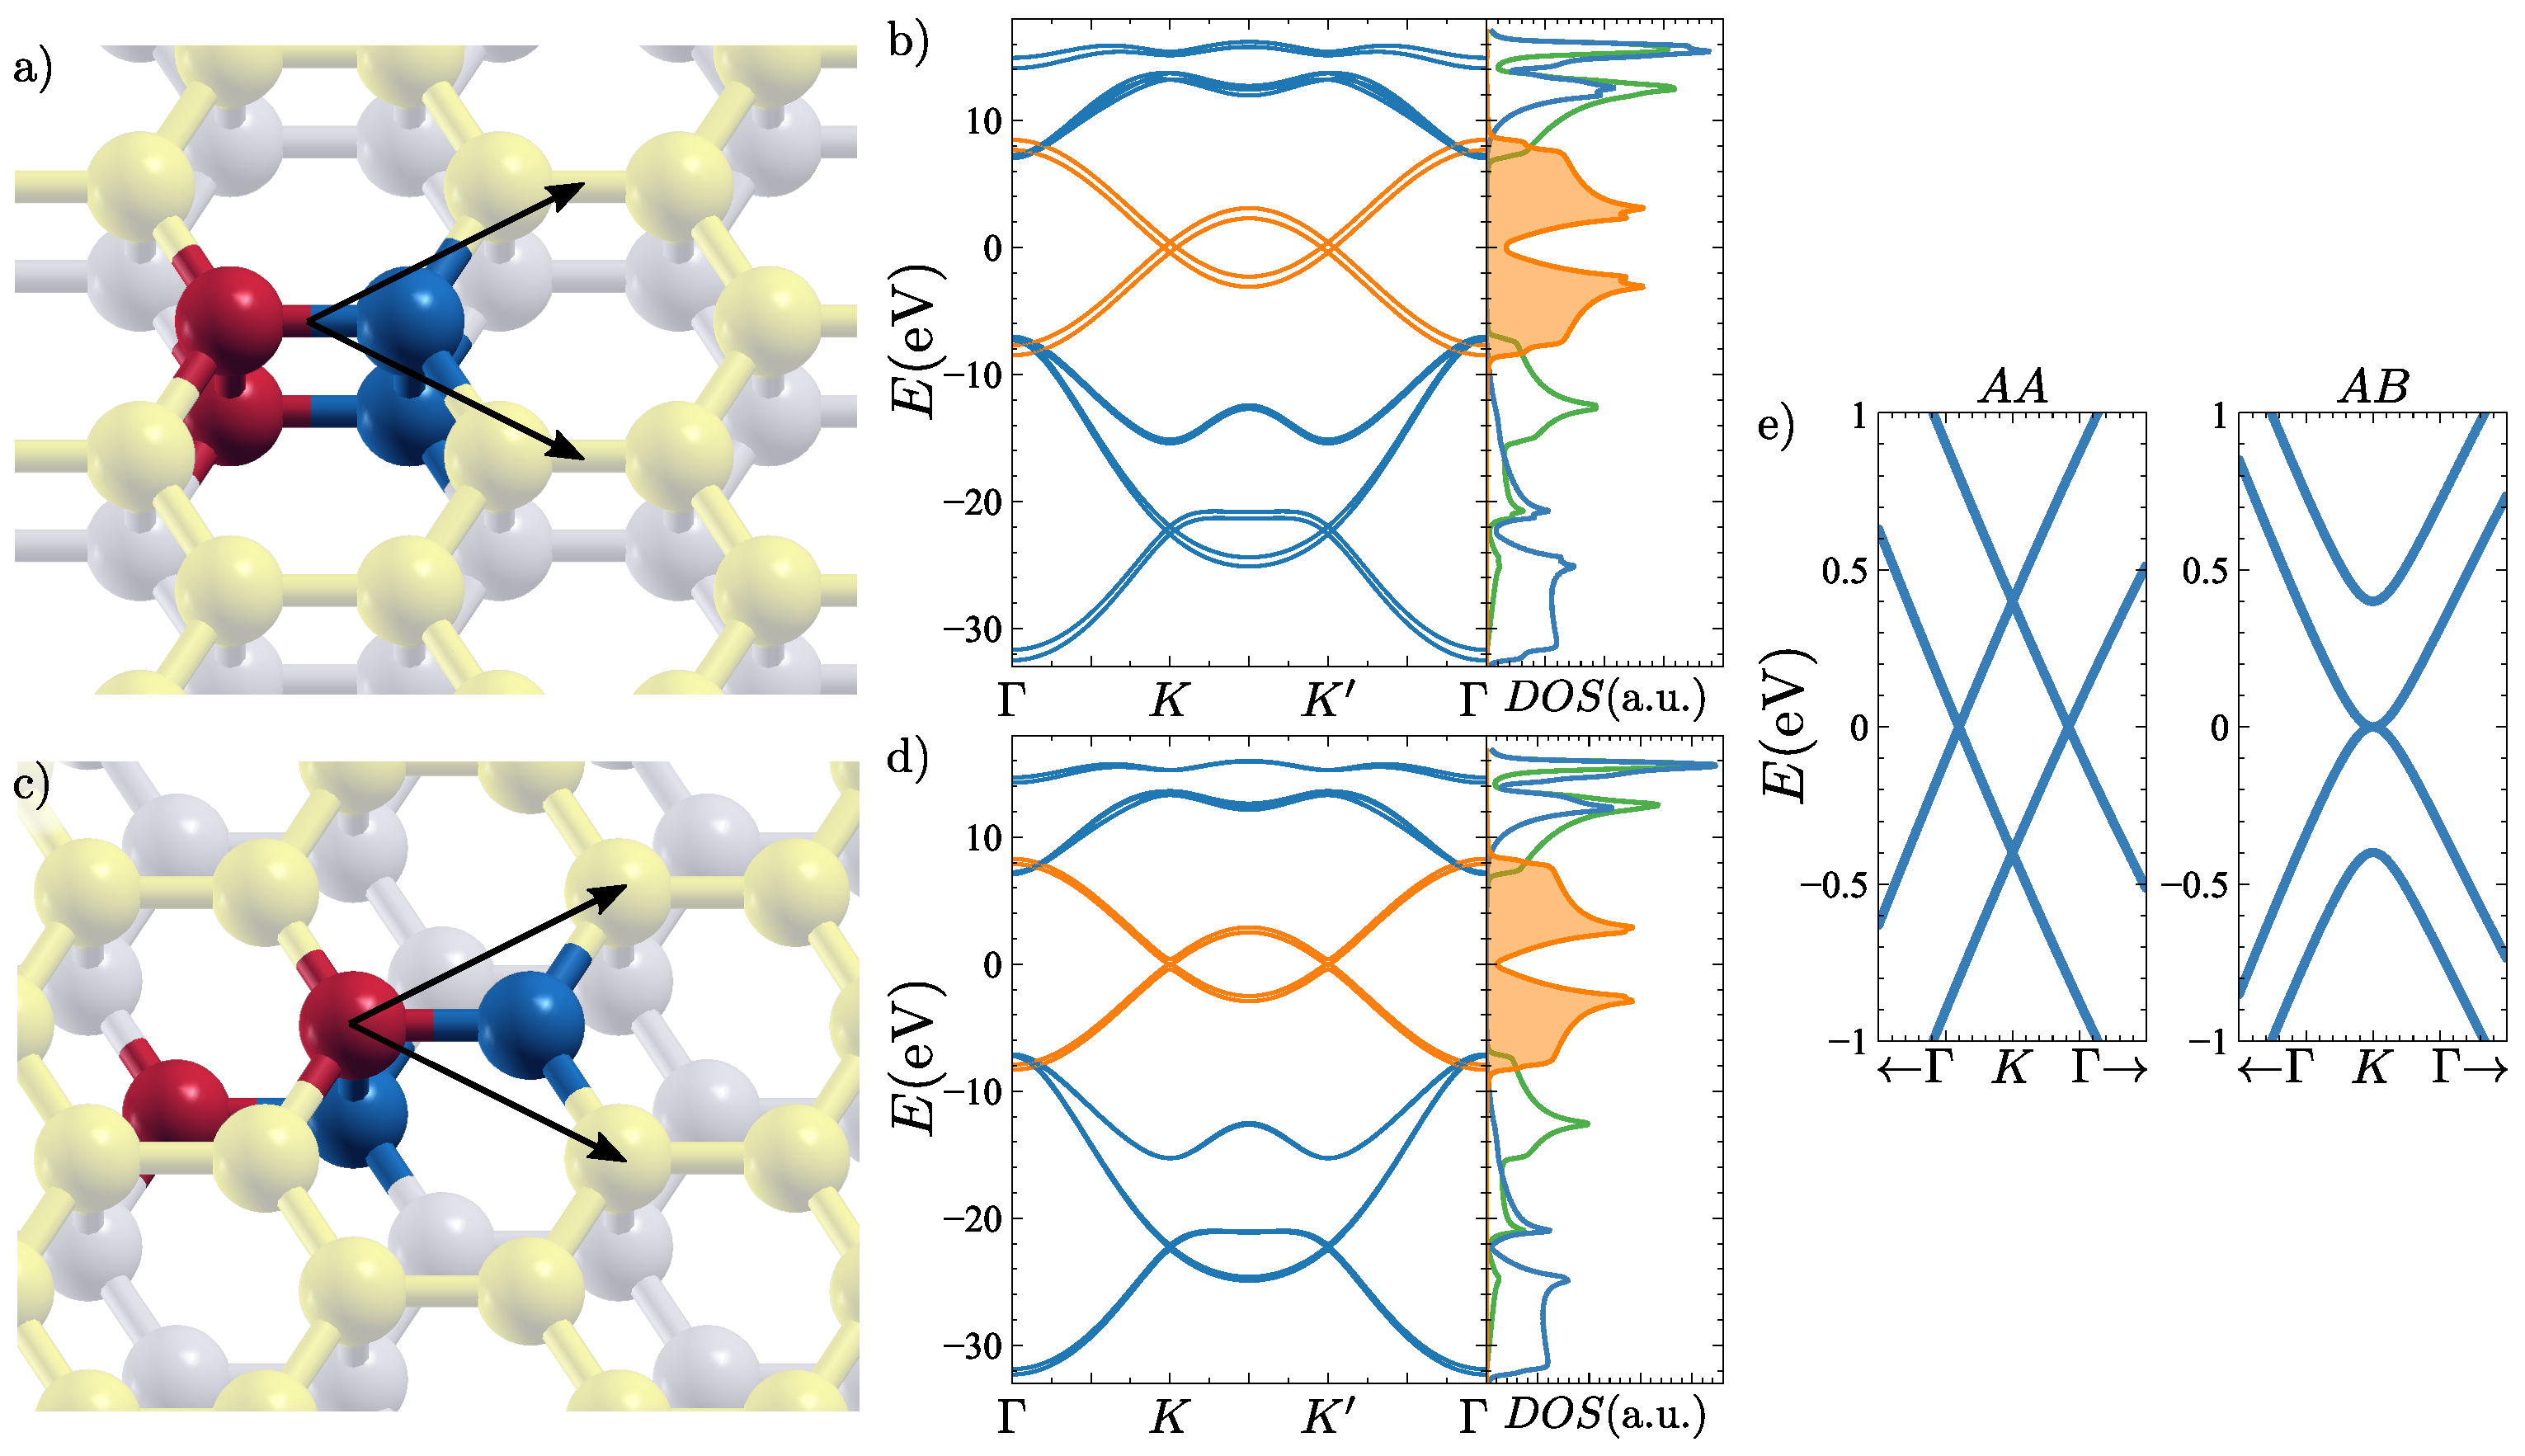
\includegraphics{graphene_bilayer/figures/bilayer_stackings.pdf}
\vspace{-20pt}
\caption{a,b) Cartoon depiction of the atomic structure of bilayer graphene in $AA$-stacking and band structure of $AA$-stacking respectively. c,d) Cartoon depiction of the atomic structure of bilayer graphene in $AB$-stacking and band structure of $AB$-stacking respectively. e) Comparison of the $AA$ and $AB$ stackings in the band structure around the $K$ point.}
\label{Gbi_stack}
\end{figure}
\FloatBarrier
%~~~~~~~~~~~~~~~~~~~~~~~~~~~~~~~~~~~~~~~~~~~~~~~~~~~~~~~~~~~%
At first glance it may seen that both stackings result in a very similar band structure. The main differences happen around the $K$ ($K'$) points as it is shown in \fref{Gbi_stack}e).

%In order to understand these band structures we can start with two decoupled graphene layers, and then turn on the interlayer hopping via an adiabatic parameter $\eta\in[0,1]$.

In order to understand these band structures we can restrict ourselves to analyze the $\vec{k}=K$ point. In this point the $\vec{k}$ dependence vanishes, $f(K)=0$. So the Hamiltonian \eqref{Gbi} reads:

\begin{equation}
   H^{AA}(K) = \left(\begin{array}{cccc}
         0 & 0 & t' & 0 \\
         0 & 0 & 0 & t' \\
         t' & 0 & 0 & 0 \\
         0 & t' & 0 & 0
   \end{array}\right)\quad;\quad
   H^{AB}(K) = \left(\begin{array}{c|cc|c}
         0 & 0 & 0 & 0 \\ \hline
         0 & 0 & t' & 0 \\
         0 & t' & 0 & 0 \\ \hline
         0 & 0 & 0 & 0
   \end{array}\right)
\label{HK}
\end{equation}

When $\eta=0$ the band structure is just that of graphene, but twofold, so at the $K$ point there are 4 degenerate states.
For $\eta>0$, in the $AA$-stacking, every atom interacts with another atom from the other layer it is obvious from \eqref{HK} that there will be no states at $E=0$ but rather two degenerate states at $E=\pm t'$.
%, it is to be expected a bonding-antibonding-like splitting for every $\vec{k}$, in fact that is exactly what happens, and vertical rigid shift of the band structure. Around the $K$ point this translates in having two cones placed at $E=\pm t'$.

In the $AB$-stacking only one of the atoms of each layer interacts via $t'$, at the $K$ point two states will remain at $E=0$, while the other will be shifted to $E=\pm t$.
%, one could think that around the $K$ point one of the cones hybridizes into a bonding-antibonding splitting and it would remain a cone with two gapped pseudo-cones at $E=\pm t'$, but the calculation does not yield exactly that, but rather a ``parabolized'' version of this scenario. The parabolic component comes from second order hoppings between the two layers.\\

%in the basis $\mathcal{B}=\left\{\ket{\phi^A_{1}}, \ket{\phi^B_{1}}, \ket{\phi^A_{2}}, \ket{\phi^B_{2}}\right\}$, where the numbers label the layer and the letters label the sublattices.
%By rearranging the basis into $\mathcal{B}=\left\{\ket{\phi^A_{1}}, \ket{\phi^A_{2}},\ket{\phi^B_{1}}, \ket{\phi^B_{2}}\right\}$ it can be shown that the $H^{AB}_0$ shows two vanishing subspaces while $H^{AA}_0$ does not:
%\begin{equation}
%   H^{AA}_0 = \left(\begin{array}{cccc}
%         0 & t' & t & 0 \\
%         t' & 0 & 0 & t \\
%         t & 0 & 0 & t' \\
%         0 & t & t' & 0
%   \end{array}\right)\quad;\quad
%   H^{AB}_0 = \left(\begin{array}{cc|cc}
%         0 & 0 & t & 0 \\
%         0 & 0 & t' & t \\ \hline
%         t & t' & 0 & 0 \\
%         0 & t & 0 & 0
%   \end{array}\right)
%\end{equation}
%For the $AA$ case, \eqref{HK}, will present two degenerate states at $E=\pm t'$ showing no states at $E=0$ \emph{at the $\vec{k}=K$ point}. This is not the case for the $AB$-stacking. Since only one of the sublattices of each layer is connected to the other layer, two states should remain at $E=0$ while the other two should split by $E=\pm t$
%\medbreak



Since the $AB$-stacking is the most common one, and the most appropriate for our goals, we will focus the rest of the discussion in this kind of stacking.\\


The description for the Bernal stacking is not much different from that of graphene: the Bravais lattice is still a triangular lattice with lattice vectors described by \eqref{latt_vec}, hence the \ac{fbz} is the same. The main difference is that the minimal basis now has four atomic positions.
%~~~~~~~~~~~~~~~~~~~~~~~~~~ FIGURE ~~~~~~~~~~~~~~~~~~~~~~~~~%
\begin{figure}[h!]
\centering
\includegraphics{graphene_bilayer/figures/graphene_bi_summary.pdf}
\vspace{-5pt}
\caption{a) Cartoon depiction of the atomic structure of bilayer graphene using the lattice vectors defined in \eqref{latt_vec}. b) Band structure of bilayer graphene. Notice the c) Comparison of the band structure and \ac{dos} in the presence of an external electric field.}
\label{Gbi_summary}
\end{figure}
\FloatBarrier
%~~~~~~~~~~~~~~~~~~~~~~~~~~~~~~~~~~~~~~~~~~~~~~~~~~~~~~~~~~~%
In bilayer graphene the $p_z$ manifold is no longer decoupled from the other orbitals since there are hopping processes between the $p_z$ orbitals in one layer and the $s$ orbitals in the other layer. Nevertheless the $p_x$ and $p_y$ still have no direct hopping with the $p_z$ orbitals.
While it is true that the symmetry protecting the $p_z$ manifold is broken in this system, the fact remains that at low energy and around the $K$ points the $p_z$ description is enough (and exactly at the Dirac points it is an exact description).\\

There are several ways in which we can stack several graphene layers. Until further notice we will consider only Bernal stacking, meaning that only one of the sublattices of one layer is connected to the opposite sublattice of the other layer. This configuration results in having in each layer one sublattice which is ``\emph{connected}'' and another that lays on ``\emph{hollow}'' sites (\fref{Gbi_summary}{a)}).

We can approach bilayer graphene by considering two decoupled layers of graphene. In this case we would have twice the typical graphene band structure, one for each layer. When the interlayer coupling is switched on (see \eqref{Gbi}) two of the bands split from the rest according to the interlayer hopping $t'$ and the other two become parabolic.\\

In order to account for this new hoppings we keep the \ac{sk} model and simply scale the graphene parameters so that the interlayer $p_z$ hopping takes the value $t'=\SI{0.4}{\meV}$. So, the \ac{sk} parameter can be obtained simply by multiplying the parameters in \ref{G_SK_params} by the factor $f\sim0.05$


\section{electric field}
It is well known that the band structure of bilayer graphene changes dramatically in the presence of an external electric field\cite{McCann2006, Castro2007, Oostinga2007, Zhang2009, Taychatanapat2010, Castro2010a, Ponomarenko2011, Allen2012, Sui2015}.
The application of an electric field has several effects in the electronic structure of the system.

The most obvious effect is the different shift of the on-site energies for each layer. This effect breaks the bipartite-ness of the system and results in a tunable band gap as reported by many experiments.

Another effect is the possible doping of the system. By simply gating bilayer graphene we would be introducing a lot of carriers resulting in huge filling factors. This problem/feature can be address and, in fact used to our advantage by using dual-gating rather than a single gate as we will see in the following sections.

Finally, the last effect is the appearance of a Rashba-like term due to the deformation of the atomic orbitals which could open both $s-p_z$ hoppings and a spin flip channel (when combined with the \ac{soc}).


\subsection{Gap opening}
The effect of an electric field in the electronic structure is just a layer dependent shift in the on-site energies of the atomic orbitals. In particular, in the basis \eqref{basis_bi}, it can be written as
\begin{equation}
   H_\mathcal{E} = \mathcal{E}\Lambda = \left(
   \begin{array}{cc|cc}
     \mathcal{E} & 0 & 0 & 0\\
     0 & \mathcal{E} & 0 & 0\\ \hline
     0 & 0 & -\mathcal{E} & 0\\
     0 & 0 & 0 & -\mathcal{E}\\
   \end{array}\right)
\label{Helec}
\end{equation}
where $\Lambda$ is the layer operator and $\mathcal{E}$ the strength of the electric field.

In particular, a band gap is open at the Dirac points as shown in \fref{Gbi_summary}{c)}. Along with this effect, there are other processes not captured by the model, for instance a strong redistribution of the charge will take place in the system, polarizing the two layers in opposition to the applied electric field. This screening process has be addressed in the literature showing that its main effect is a Hartree renormalization of the gap\cite{McCann2006,Wang2016a}. While this effects are certainly not negligible we can adopt an empirical approach based on the experimental observation\cite{Zhang2009, Taychatanapat2010} of a gap up to $\Delta=\SI{250}{\meV}$, regardless of the real voltage required to achieve it.



\subsection{Doping}
%~~~~~~~~~~~~~~~~~~~~~~~~~~ FIGURE ~~~~~~~~~~~~~~~~~~~~~~~~~%
\begin{figure}[h!]
\centering
\includegraphics[width=0.5\textwidth]{graphene_bilayer/figures/dual_gate.pdf}
\vspace{-5pt}
\caption{Schematics of dual gating.}
\label{dual_gate}
\end{figure}
\FloatBarrier
%~~~~~~~~~~~~~~~~~~~~~~~~~~~~~~~~~~~~~~~~~~~~~~~~~~~~~~~~~~~%
The doping (extra charge absorbed into the system) in the graphene bilayer can  be estimated simply by applying Gauss' law:
\begin{equation}
   \diver{D} = \rho-\rho_0 = \rho_f
\label{gauss}
\end{equation}
where $\rho$ is total charge density, $\rho_0$ is the bounded charge density so that $\rho_f$ is the free charge density.

The dual-gating setup can be considered as an infinite capacitor, hence, the electric field only has $z$ component, hence the divergence of the displacement results in a derivative which can be discretized:
\begin{equation}
   \diver{D}=\frac{\partial D}{\partial z} =\frac{D_t-D_b}{dz} = \rho_f =
   e\frac{N}{V} \Rightarrow D_t-D_b = e\delta n
\label{doping}
\end{equation}
where $N$ and $V=Adz$ are the number of electrons and volume respectively ($A$ is the area), and $\delta n$ is the bidimensional density of electrons.

In order to calculate the potential difference between the two graphene layers, we can consider simply the average of the electric field inside the capacitor:
\begin{equation}
   \Delta V = \langle\vec{E}\rangle \Delta z = \frac{E_t+E_b}{2} \Delta z=
   \frac{\Delta z}{2} \left(\frac{D_t}{\varepsilon_t} +
                            \frac{D_b}{\varepsilon_b} \right)
\label{potential}
\end{equation}
where $\Delta z$ is width of the graphene bilayer and $\varepsilon_t$ and       $\varepsilon_b$ are the electric permeability of the top and bottom             dielectrics. $D_t$ and $D_b$ are (the $z$-component of) the displacement fields in the top and bottom regions.
\begin{equation}
   D_t = \frac{\varepsilon_t}{d_t}\left(V_{t}-V^0_{t}\right) \qquad;\qquad
   D_b = \frac{\varepsilon_b}{d_b}\left(V_{b}-V^0_{b}\right)
\end{equation}
where $V^0_{t/b}$ are the off-set potential required to have charge neutrality, usually referred to as \ac{cnp}.

Equations \eqref{doping} and \eqref{potential} show that by choosing the        appropriates $V_t$ and $V_b$ we can independently change the doping of the      system and the gap opened in the band structure.





\subsection{Rashba}
Another effect is the mixing of the $p_z$ with the other orbitals. The presence of the electric field deforms the atomic orbitals breaking the symmetries present in the purely hydrogenic orbitals. In particular a new intra-atomic hopping $p_z$ and the $p_{x/y}$ orbitals appear. The application of an electric field leads to the appearance of an intrinsic Rashba and \ac{soc} similar to the terms proposed by Kane and Mele\cite{Kane2005}.
Following the calculations in %\citef{Min2006}
\cite{Min2006} we can see that the relation between the applied electric field and the effective intra-atomic Rashba follow the equation:
\begin{equation}
   \lambda_R=\frac{e\mathcal{E}z_0}{3V_{sp\sigma}}\xi \qquad;\qquad
   \lambda_{SOC}=\frac{|E_{s}|}{18V^2_{sp\sigma}}\xi^2
\label{rashba}
\end{equation}
where $\xi\sim\SI{6}{\meV}$ is the atomic carbon spin-orbit coupling strength
which for a typical electric field of $\mathcal{E}\sim\SI{50}{\V}/\SI{300}{\nm}$ result in an effective Rashba coupling $\lambda_R\sim\SI{0.011}{\meV}$ and the \ac{soc} $\lambda_{SOC}\sim\SI{0.0011}{\meV}$.

These terms, are in the scale of $\SI{e-2}{\meV}$ while the gap open can reach up to $\SI{2.5e2}{\meV}$ so we will neglect these interactions from now on.


\section{Spin proximity}
Another way to interact with the spin degree


\section{Kink states}
An interesting feature of this system appears when we applied an electric field of different sign in different regions of the system. The opening of an opposite gap in two different regions leads to the appearance of kink states in the interface. In addition to its experimental observation\cite{Li2016}, we can provide a quick example of these states.

We consider an 2d sheet of bilayer graphene which has $\mathcal{E}>0$ for atomic positions with $x>0$ and $\mathcal{E}<0$ otherwise.
%~~~~~~~~~~~~~~~~~~~~~~~~~~ FIGURE ~~~~~~~~~~~~~~~~~~~~~~~~~%
\begin{figure}[h!]
\centering
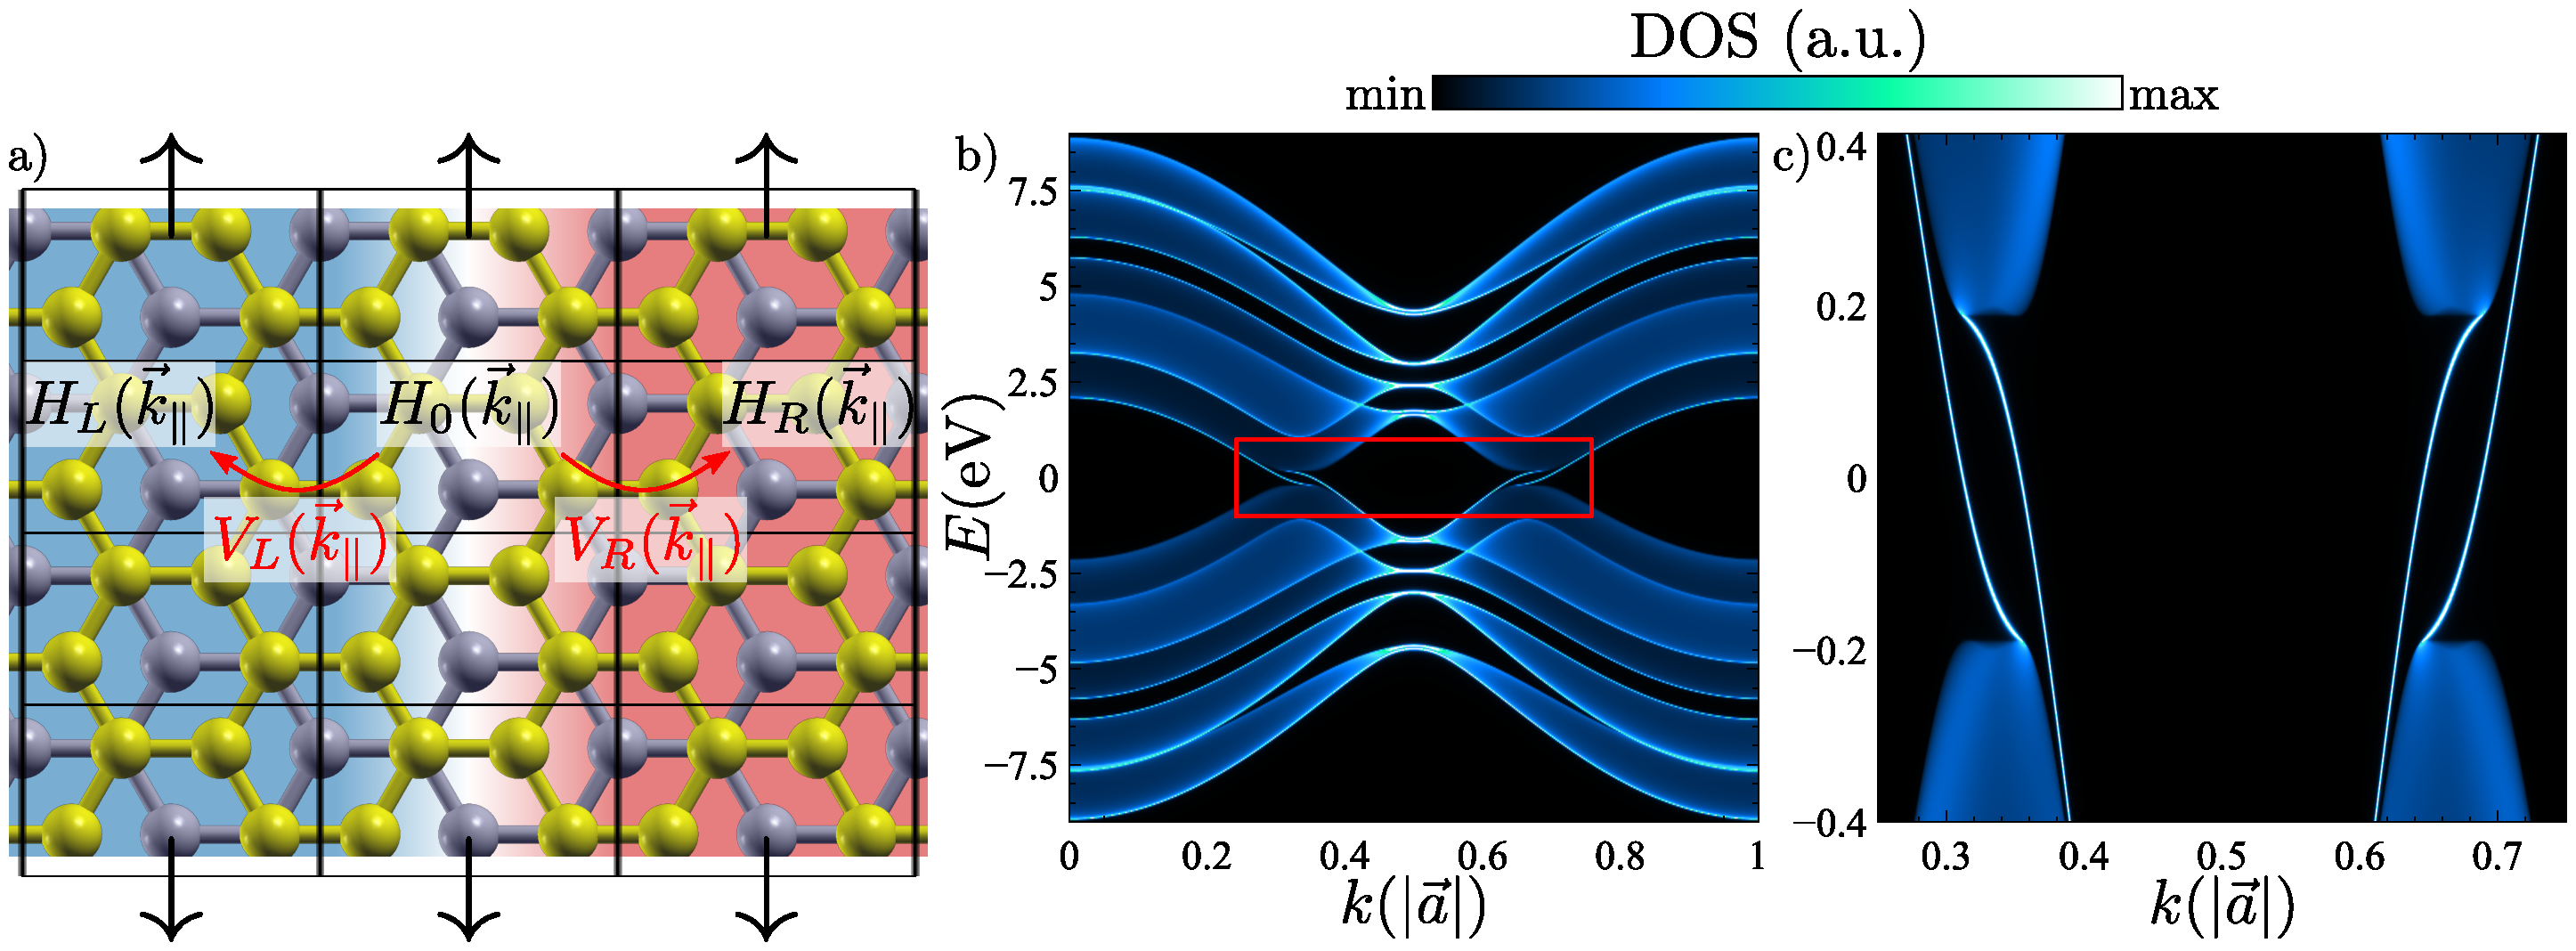
\includegraphics{graphene_bilayer/figures/kink_states.pdf}
\vspace{-5pt}
\caption{a) schematic of the system hosting kink states. b) \ac{dos} over the whole Brillouin Zone. c) Zoom around the Dirac cones.}
\label{kink_states}
\end{figure}
\FloatBarrier
%~~~~~~~~~~~~~~~~~~~~~~~~~~~~~~~~~~~~~~~~~~~~~~~~~~~~~~~~~~~%
In order to study the states at the interface between these two regions we consider the Green's function for the interface:
\begin{equation}
  G(E,k_{\parallel}) = \frac{1}{E+i\epsilon-H_0(k_\parallel)-\Sigma_R(k_\parallel)-\Sigma_L(k_\parallel)}
\end{equation}
where each self-energy $\Sigma_\alpha$ with $\alpha\in\{L/R\}$ can be calculated by solving iteratively the coupled equations:
\begin{equation}
\begin{split}
  \Sigma_\alpha(E,k_\parallel) &= V_\alpha(k_\parallel)g_\alpha(E,k_\parallel)V^{\dagger}_\alpha(E,k_\parallel) \\
  g_\alpha(E,k_\parallel) &= \frac{1}{E-H_\alpha(k_\parallel)-\Sigma_\alpha(E,k_\parallel)}
\end{split}
\end{equation}
Once the Green's function is calculated, the \ac{dos} is calculated as usual as:
\begin{equation}
   \rho(E,k_\parallel) = \frac{-1}{\pi}\Im{G(E,k_{\parallel})}
\end{equation}







%%   \newpage
%%   %Kane's proposal~\cite{Kane1988}, and all the experimental realizations of it~\cite{Morello2010}, based the control of the Qubits in the manipulation of the electronic states with an electric gate that would modify the electronic cloud around the $^{31}P$ nucleus.
%%   %
%%   %Since graphene is a purely \ac{2dm} its electronic properties are highly tunable by proximity, electric gating or other techniques. First we make a quick review of the properties of \ac{gb} and the effect of an external electric field and then we explore the possibility of the realization of 1 and 2-Qubit operations.
%%   %
%%   %\section{Graphene Bilayer}
%%   %The minimal unit cell for describing \ac{gb} contains four atoms, disposed as seen in the inset in Fig.~\ref{bilayer}. The lattice vectors describing the Bravais lattice are the same as in the case of monolayer graphene (see Sec.~\ref{ch:graphene}). Since the interlayer distance, is  around three times bigger than the C-C distance, $d_\text{inter} \sim \SI{3.3}{\angstrom}$ (from literature~\cite{Charlier1994a,Lam2008,Brihuega2012}), it is expected that the interlayer hopping will be smaller, in fact from literature~\cite{KatsnelsonBook} we get that the interlayer hopping $t'\simeq 0.15\cdot t_{\pi-\pi}\simeq\SI{0.4}{\eV}$
%%   %The effect of the interlayer interaction is to ``parabolize'' the linear bands around the $K$ points and double the $p_z$ manifold bands.
%%   %%~~~~~~~~~~~~~~~~~~~~~~~~~~ FIGURE ~~~~~~~~~~~~~~~~~~~~~~~~~%
%%   %\begin{figure}[h!]
%%   %\centering
%%   %\includegraphics{chapter06/figures/bilayer_bandDOS.pdf}
%%   %\vspace{-5pt}
%%   %\caption{Band structure and \ac{dos} of bilayer graphene along the $\Gamma-K-K'-\Gamma$ path and density of states. The red shadowed region shows the contribution of the $p_z$ manifold, \emph{almost} decoupled from the other orbitals.}
%%   %\label{bilayer}
%%   %\end{figure}
%%   %\FloatBarrier
%%   %%~~~~~~~~~~~~~~~~~~~~~~~~~~~~~~~~~~~~~~~~~~~~~~~~~~~~~~~~~~~%
%%   %The $p_z$ bands at the $K$ point are split by an amount proportional to the interlayer hopping
%%   %
%%   %Notice that in the bilayer the $p_z$ manifold is no longer decoupled from the rest of the orbitals (for instance there is a finite hopping between $p_z$ orbitals from one layer and $s$ orbitals of the other), nevertheless close to the Fermi energy the approximation of considering only $p_z$ orbitals is still justified.
%%   %The general aspect of the \ac{dos} is similar to that of the graphene but it is important to notice that at $E=0$ the \ac{dos} is now finite.
%%   %
%%   % \section{Effect of the electric field}
%%   %The main effect of an external electric field applied to bilayer graphene is to shift the (on-site) energy of the electrons, we can write such a Hamiltonian term like
%%   %% external potential energy
%%   %
%%   %\begin{equation}
%%   %  H_{\vec{E}} = \lambda_e q_e \vec{d} \widehat{E} %\sum_i \varepsilon_l \crea{c}{i}\des{c}{i}
%%   %\end{equation}
%%   %where $\lambda_e$ is the magnitude of the external electric field, $\vec{d}$ is the interlayer distance, and $\widehat{E}$ is the electric field along the interlayer direction.
%%   %% where $E$ is an external electric field along the direction and d is the interlayer separation of bilayer graphene.
%%   %% where $\varepsilon_l=\pm1$ depending on the layer, $l$,  of the atom $i$.
%%   %
%%   %The effect of such a term in \ac{gb} is just to open a gap~\cite{Zhang2009,Yamashiro2012,Brihuega2012,Lam2008,Min2007} close to the Fermi energy as shown in fig~\ref{bi_Efield}.
%%   %
%%   %%~~~~~~~~~~~~~~~~~~~~~~~~~~ FIGURE ~~~~~~~~~~~~~~~~~~~~~~~~~%
%%   %\begin{figure}[h!]
%%   %  \centering
%%   %  \includegraphics[width=\textwidth]{chapter06/figures/bilayer_elec.pdf}
%%   %  \vspace{-10pt}
%%   %  \caption{\ac{dos} of a bilayer graphene system in the absence (left panel) and presence (right panel) of an electric field $E=\SI{0.5}{\eV}$.} %XXX UNITS
%%   %  \label{bi_Efield}
%%   %\end{figure}
%%   %\FloatBarrier
%%   %%~~~~~~~~~~~~~~~~~~~~~~~~~~~~~~~~~~~~~~~~~~~~~~~~~~~~~~~~~~~%
%%   %
%%   % Analogously to the discussed scenario of a vacancy in (monolayer) graphene, the introduction of a vacancy also results in the appearance of a ``zero energy state''. In the presence of an external electric field the impurity state will not appear at $E=0$ but shifted in energy as shown in fig.~\ref{dos_bi_dfct}
%%   
%%   % %~~~~~~~~~~~~~~~~~~~~~~~~~~ FIGURE ~~~~~~~~~~~~~~~~~~~~~~~~~%
%%   % \begin{figure}[h!]
%%   % \centering
%%   % \includegraphics{chapter06/figures/bilayer_dos_dfct.png}
%%   % \vspace{-5pt}
%%   % \caption{\ac{dos} of bilayer graphene with (green line) and without (blue line) a vacancy in the presence of an external electric field. The left and right panels have been calculated for electric fields of opposite sign, notice that }
%%   % \label{dos_bi_dfct}
%%   % \end{figure}
%%   % \FloatBarrier
%%   % %~~~~~~~~~~~~~~~~~~~~~~~~~~~~~~~~~~~~~~~~~~~~~~~~~~~~~~~~~~~%
%%   
%%   % \subsection{About the charge neutrality}
%%   % when a bias is applied to \ac{gb} there is the chance that some charge is transferred form one layer to the other\cite{Wang2016a,Zhang2009}. To be sure of how relevant this effect is we calculate where the Fermi Energy lies as well as the charge in each layer.
%%   
%%   
%%   
%%   % % The position where the adatom is introduced now is important since one of the sublattices of each layer is fully connected to the other layer. All the possibilities for the H chemisorption are depicted in figure\red{FIG}. We will consider only the structure (b).
%%   % %
%%   % % %~~~~~~~~~~~~~~~~~~~~~~~~~~ FIGURE ~~~~~~~~~~~~~~~~~~~~~~~~~%
%%   % % \begin{figure}[h!]
%%   % % \centering
%%   % % \includegraphics{chapter06/figures/bilayer_H.pdf}
%%   % % \vspace{-5pt}
%%   % % \caption{All opssible atomic strucutre for chemisorbed H}
%%   % % \end{figure}
%%   % % %~~~~~~~~~~~~~~~~~~~~~~~~~~~~~~~~~~~~~~~~~~~~~~~~~~~~~~~~~~~%
%%   % %
%%   % %
%%   % %
%%   % % \subsection{Electric control of the hyperfine interaction}
%%   % % Electric control of the hyperfine with the bias in the bilayer.
%%   % % %~~~~~~~~~~~~~~~~~~~~~~~~~~ FIGURE ~~~~~~~~~~~~~~~~~~~~~~~~~%
%%   % % \begin{figure}[h!]
%%   % % \centering
%%   % % \includegraphics{chapter06/figures/hyperfine.png}
%%   % % \vspace{-5pt}
%%   % % \caption{Hyperfine dependence with the bias voltage.}
%%   % % \end{figure}
%%   % % \FloatBarrier
%%   % % %~~~~~~~~~~~~~~~~~~~~~~~~~~~~~~~~~~~~~~~~~~~~~~~~~~~~~~~~~~~%
%%   % %
%%   % % A similar behavior can be seen from the gap.
%%   % % %~~~~~~~~~~~~~~~~~~~~~~~~~~ FIGURE ~~~~~~~~~~~~~~~~~~~~~~~~~%
%%   % % \begin{figure}[h!]
%%   % % \centering
%%   % % \includegraphics{chapter06/figures/gap.png}
%%   % % \vspace{-5pt}
%%   % % \caption{Dependence of the gap and the energy of the resonance with the bias voltage.}
%%   % % \end{figure}
%%   % % \FloatBarrier
%%   % % %~~~~~~~~~~~~~~~~~~~~~~~~~~~~~~~~~~~~~~~~~~~~~~~~~~~~~~~~~~~%
%%   % %
%%   % %
%%   \section{1 Hydrogen adatom}
%%   \subsection{General considerations} %~~~~~~~~~~~~~~~~~~~~~~~~~~~~~~~~~~~~~~~~~~%
%%   To study hydrogrnation of graphene bilayer we will consider a hexagonal armchair island big enough for the splitting among energy levels to be negligible compared with the splitting opened due to the external electric field.
%%   
%%   To study these systems we will consider a basis of localized states that could be considered to be the $p_z$ hydrogenoid orbitals.
%%   \begin{equation}
%%     \mathcal{B} = \left\{\phi_1,\phi_2,\dots,\phi_\beta,\dots,\phi_{N_C}\right\}
%%   \end{equation}
%%   
%%   Written in such a basis, the general Hamiltonian and its eigenvectors, then, will look like
%%   \begin{equation}
%%     H = H_t + H_{\lambda_E} \quad\quad;\quad\quad
%%     H\ket{\psi_\alpha} = E_\alpha\ket{\psi_\alpha} \quad\quad;\quad\quad
%%     \ket{\psi_\alpha} = \sum_\beta c_\beta\ket{\phi_\beta}
%%   \label{general}
%%   \end{equation}
%%   
%%   
%%   The term $H_t$ represents the kinetic energy arising from the hopping between neighboring sites and the term $H_{\lambda_E}$ corresponds to the effect of an external electric field on the electrons. Such a term takes the form:
%%   \begin{equation}
%%     H_{\lambda_E} = \lambda_E
%%     \left(\begin{array}{cc}
%%     \mathds{1} & 0 \\
%%     0 & -\mathds{1}
%%     \end{array}\right)
%%   \end{equation}
%%   where we use the identity elements $\pm\mathds{1}$ to account for spin, orbitals and any oder degree of freedom. The sign $\pm$ is decided with respect to the layer.
%%   
%%   The vacancies are introduced in this model as an infinite on-site energy for the chosen atom(s). Unless otherwise stated everything is done in $\si{\eV}$ %$eV$
%%   , \emph{not hopping units}, the $p_z$-$p_z$ hopping is chosen as $t=\SI{-2.7}{\eV}$.
%%   
%%   
%%   
%%   
%%   
%%   \subsection{Note on the geometry}
%%   Any vacancy considered will always be chosen on a hollow position (see fig~\ref{geo_sketch} $c)$) even if it not specified in the text. When only one vacancy is considered, it will be placed at the hollow atomic position closest to the center of the island.
%%   
%%   When two vacancies are considered they will be placed as separated from the edges as possible, as shown in fig~\ref{geo_sketch} $b)$ since this configuration allows the study of a wider range of the relative angle and distance ($\alpha$ and $d$).
%%   % Later in the text another configuration consisting in one vacancy in the center of the island, and the other in different positions $\vec{r}=d\cos(\alpha)+d\sin(\alpha)$.
%%   %~~~~~~~~~~~~~~~~~~~~~~~~~~ FIGURE ~~~~~~~~~~~~~~~~~~~~~~~~~%
%%   \begin{figure}[h!]
%%   \centering
%%   \includegraphics[width=\textwidth]{chapter06/figures/vacs_sketch.pdf}
%%   \vspace{-15pt}
%%   \caption{$a)$ and $b)$ show sketches of the position of the vacancies and relevant geometric information. In the upper left corner the real atomic structure is shown using blue for the lower layer and red for the upper one. The length $L_C$ is the typical size of the in-gap state. $c$ atomic structure showing the ``connected'' and ``hollow'' sites in the upper layer as well as the $A/B$ sublattices (in red/blue).}
%%   \label{geo_sketch}
%%   \end{figure}
%%   \FloatBarrier
%%   %~~~~~~~~~~~~~~~~~~~~~~~~~~~~~~~~~~~~~~~~~~~~~~~~~~~~~~~~~~~%
%%   
%%   Note that as long as the border effects are negligible, and due to the $C_3$ symmetry of the in-gap states in graphene, we only need to explore the range of angles between vacancies of $\alpha\in\left[0,\tfrac{\pi}{3}\right]$.
%%   
%%   
%%   \subsection{Single vacancy} %~~~~~~~~~~~~~~~~~~~~~~~~~~~~~~~~~~~~~~~~~~~~~~~~~~%
%%   Since we are studying an island with a single vacancy, the energy levels are a discrete set of energies. In figure~\ref{1vac_spec}~c) the difference in the spectrum due to the introduction of a vacancy at $\lambda_E=0$ is shown. When a vacancy is introduced, an in-gap state appears at $E=0$ and some \emph{(quasi-)}degeneracies are broken.
%%   
%%   The effect of the electric field in the spectrum is shown in figure~\ref{1vac_spec} $a)$ and $b)$. Its main effect is to open a gap, linearly dependent with the electric field.
%%   
%%   The shift in the energy at which the in-gap state appears is linear for low electric field, but it remains in-gap for all the regime of electric fields studied. In fig~\ref{1vac_spec} $a$-$c)$ only the eight eigenvalues closest to $E=0$ are plotted. Nevertheless, since the spacing between levels is much smaller than the gap open by the electric field, they appear grouped in two sets of almost-degenerate energies, one at $E>0$ and the other at $E<0$.\\
%%   
%%   %~~~~~~~~~~~~~~~~~~~~~~~~~~ FIGURE ~~~~~~~~~~~~~~~~~~~~~~~~~%
%%   \begin{figure}[!ht!]
%%   \centering
%%   \includegraphics[width=\textwidth]{chapter06/figures/single_vac_spectrum.pdf}
%%   \vspace{-15pt}
%%   \caption{$a)$ and $b)$ show the pristine and defected spectrum respectively as a function of different applied electric fields. Notice the opening of a gap linear with the electric field (in both the pristine and defected cases) and the appearance of an extra state inside the gap. $c)$ Pristine (red) and defected (blue) spectrum for the case of no electric field $\lambda_E=0$. Panel $d)$ shows four snapshots of an island ($N_C=91812$ atoms) at different values of the electric field. The black circle in panel $d)$ shows the confinement length $L_C$ defined in the text.}
%%   \label{1vac_spec}
%%   \end{figure}
%%   \FloatBarrier
%%   %~~~~~~~~~~~~~~~~~~~~~~~~~~~~~~~~~~~~~~~~~~~~~~~~~~~~~~~~~~~%
%%   
%%   In Fig~\ref{1vac_spec} $d)$ we show four snapshots of the spatial distribution of the in-gap state for different electric fields. The actual lattice of the island is shown as black dots (probably indistinguishable because of the size of the image).
%%   On top of each atomic position the weight of the wave function ($|c_\beta|^2$ using the notation of eq.~\eqref{general}) is plotted in blue/red for the lower/upper layer.
%%   On top of all this, the site of the vacancy is marked with a blue triangle.
%%   As a visual guide the confinement length (defined later) is plotted as a black circle with diameter $2L_C$.\\
%%   
%%   At $\lambda_E=0$ the system is bipartite so, according to the Lieb's theorem\cite{Lieb1989}, after the removal of one site, a sublattice-polarized state should appear at $E=0$. This is exactly what happens as shown in Fig.~\ref{1vac_spec}.
%%   
%%   When we study the real-space distribution of the in-gap state we find that in the absence of electric field ($\lambda_E=0$) the state is spread all over the island, Fig.~\ref{1vac_spec} $d)$, no matter the size of the island (see Fig.~\ref{IPR_lc} $a)$ bellow). Notice that the effect of the border is not negligible in this regime and, in fact, is the responsible of the breaking of the expected $C_3$ symmetry of the state (at long distances, close to the vacancy the $C_3$ symmetry is almost preserved).
%%   
%%   
%%   Another important aspect is that the distribution of this wave function is such that in the upper layer (the one containing the vacancy) the wave function is quite confined around the vacancy (3-6 closest atoms) and it barely changes with the electric field, whereas in the lower layer the spreading of the wave function varies from the whole space available, to a few angstroms.
%%   
%%   
%%   To study quantitatively the properties of the in-gap state $\psi_0$ we define four quantities that will be useful later on.
%%   \begin{itemize}
%%     \item \emph{Confinement length}, $L_C$, defined, hand-wavingly, as the distance at which more than $90\%$ of the state is located
%%     \begin{equation}
%%       0.9 = \int_{0}^{L_C} \psi_0(r) dr   %XXX arreglar!!!
%%       \label{loclen}
%%     \end{equation}
%%     This confinement length can be used as a measurement of the spreading of the in-gap state $\psi_0$.
%%     \item \emph{Inverse participation ratio} (IPR), $\eta$. Using the notation of equation~\eqref{general}, the IPR can be defined as:
%%     \begin{equation}
%%       \ket{\psi_0} = \sum_\beta c_\beta\ket{\phi_\beta}\quad\quad;\quad\quad
%%       \text{IPR} = \eta = \sum_i |c_\beta|^4
%%     \end{equation}
%%     \item \emph{Sublattice} and \emph{Layer polarization}, defined as the expected value of the in-gap state.
%%     \begin{equation}
%%       SP = \bra{\psi_0}\widehat{\mathcal{S}}\ket{\psi_0}
%%       \quad\quad;\quad\quad
%%       SL = \bra{\psi_0}\widehat{\mathcal{L}}\ket{\psi_0}
%%     \end{equation}
%%     where the operators $\widehat{\mathcal{S}}$ and $\widehat{\mathcal{L}}$ measure the component of a given state in a given sublattice and layer respectively. Both $SP$ and $SL$ have to be, by definition, in the closed interval $\left[-1,1\right]$.
%%   \end{itemize}
%%   
%%   In figure~\ref{IPR_lc} we study the dependence of these four properties, for different sizes of the island, as a function of the electric field.
%%   %~~~~~~~~~~~~~~~~~~~~~~~~~~ FIGURE ~~~~~~~~~~~~~~~~~~~~~~~~~%
%%   \begin{figure}[!ht]
%%   \centering
%%   \includegraphics[width=0.6\textwidth]{chapter06/figures/single_vac_properties.pdf}
%%   \vspace{-5pt}
%%   \caption{$a)$ Dependence of the localization length $L_c$ with the electric field for different sizes of the island. The dashed lines corresponds to the size of the each corresponding island. $b)$ IPR, $\eta$, dependence with the electric field for different sizes of the island. $c)$ and $d)$ show the degree of sublattice and layer polarization for different sizes of the island as a function the electric field. The values $\pm1$ refer to $A/B$ sublattice and up/down layer respectively.}
%%   \label{IPR_lc}
%%   \end{figure}
%%   \FloatBarrier
%%   %~~~~~~~~~~~~~~~~~~~~~~~~~~~~~~~~~~~~~~~~~~~~~~~~~~~~~~~~~~~%
%%   
%%   It can be seen in Fig.~\ref{IPR_lc} $a)$ that as we approach the limit $\lambda_E\rightarrow0$ the confinement length collapses to the size of the island, shown as a dashed line for each size studied. This plateau is just the effect of having an in-gap state spread all over the island.
%%   
%%   The shadowed region in all the panels shows the range of $\lambda_E$ in which the border effects can be relevant for the biggest island studied ($N_C=91812$). It is estimated as the $\lambda_E$ at which the results differ from those of the previous island. Of course it is only a rough estimation and it should be considered only as a guide to the eye when reading the results.
%%   
%%   In panel $b)$ the IPR is shown. Except for small islands the evolution of the IPR, as that of the $L_C$, is the same regardless of the size of the island. The increasing of the IPR with the electric field is another sign of the increasing localization of the in-gap state around the vacancy.\\
%%   
%%   The sublattice and layer polarization are shown in panels~\ref{IPR_lc} $c)$ and $d)$. As it can be seen at $\lambda_E=0$ the state is completely sublattice-polarized, in accordance with the Lieb's theorem, and almost layer-polarized, this ``almost'' is more easly visible in the small red component present in Fig.~\ref{1vac_spec} $d)$.
%%   
%%   As the electric field increases the bipartite character of the system is lost, in agreement with the shift of the energy of the in-gap state (no longer at $E=0$). Since the system is no longer bipartite, the sublattice polarized character of the in-gap state is no longer assured, and as shown in panel $c)$ it, in fact, decreases.
%%   
%%   The decreasing of the layer polarization is easily understood by looking at Fig.~\ref{1vac_spec} $d)$. For small $\lambda_E$ the in-gap state is mostly spread over the lower layer, while for large $\lambda_E$ the in-gap state occupies roughly the same area in both layers resulting in a $\bra{\psi_0}\widehat{\mathcal{L}}\ket{\psi_0} \rightarrow 0$
%%   
%%   % It is to be expected that if two vacancies are placed much closer than $r\sim60\text{angs}$, they could interact strongly rendering its isolation impossible even with big electric fields.
%%   
%%   
%%   
%%   \section{Double vacancy}
%%   It may be possible to control the interaction between two vacancies via an electric field by placing them at a certain distance $d$. First we are going to analyze the general phenomenology of the system studying the different states that appear as a function of the distance and angle between vacancies and the electric field.
%%   
%%   %~~~~~~~~~~~~~~~~~~~~~~~~~~ FIGURE ~~~~~~~~~~~~~~~~~~~~~~~~~%
%%   \begin{figure}[h!]
%%   \centering
%%   \includegraphics[width=\textwidth]{chapter06/figures/double_vac_spectrum.pdf}
%%   \vspace{-5pt}
%%   \caption{$a)$ and $b)$ show the pristine (red dots) and defected (blue) spectrum as a function of applied electric field. Notice the opening of a gap linear with the electric field (in both the pristine and defected cases) and the appearance of two extra states inside the gap. $c)$ Pristine (red) and defected (blue) spectrum for the case of no electric field $\lambda_E=0$. Notice that the removal of two sites (in the same sublattice) results in two states degenerate at $E=0$. The panels $1$-$8$ show a closer look ($160\times160\text{\AA}$ region) of the spatial distribution of the \emph{in-gap states} for different electric fields $\lambda_E\in\left\{-0.2,0.0,0.2\right\}$.}
%%   \label{2vac_spec}
%%   \end{figure}
%%   \FloatBarrier
%%   %~~~~~~~~~~~~~~~~~~~~~~~~~~~~~~~~~~~~~~~~~~~~~~~~~~~~~~~~~~~%
%%   
%%   In the absence of electric field, $\lambda_E = 0$, when two vacancies are introduced in the same sublattice (since both of them have to be in hollow positions) two states appear at $E=0$ in accordance to the Lieb's Theorem as shown in Fig.~\ref{2vac_spec}~$c)$. These states are sublattice-polarized and they are mostly located in the lower layer.\\
%%   
%%   When we switch on the electric field the spectrum opens a gap that increases linearly with the electric field but the two states associated with the vacancies remain inside the gap.
%%   
%%   If the vacancies are close enough to each other, the interaction between them is big enough to split these levels (originally degenerate at $E=0$) as shown in Fig.~\ref{2vac_spec} $a)$. In this case in which the vacancies are close, it is apparent from the spatial distribution of the wave functions (panels 1-8) that a pair of bonding-antibonding states is created.
%%   
%%   If the distance between the vacancies is big enough, the splitting between the in-gap states becomes negligible as shown in Fig.~\ref{2vac_spec}~$b)$.
%%   Notice that panels 5 and 6 correspond to the two in-gap eigenstates, $\psi_0$ and $\psi_1$ of the Hamiltonian which are almost degenerate in energy. For that electric field ($\lambda_E=0.2$) the confinement length of these states is smaller than the distance between the vacancies, which explains why they barely interact and are, therefore, degenerate in energy.
%%   On the other hand, panels 7 and 8 show the same eigenstates $\psi_0$ and $\psi_1$ for $\lambda_E=0.0$, it can be seen that these two state, degenerate at $E=0$ form a symmetric-antisymmetric pair of states mixing the electronic states of each of the adatoms.
%%   
%%   
%%   \subsection{Spin Exchange Interactions} %~~~~~~~~~~~~~~~~~~~~~~~~~~~~~~~~~~~~~~%
%%   Starting from the notes on the effective exchange, equations 9 and 10. I focus for now on the effective coupling $J$.
%%   
%%   Let's remember that for getting to that formula we start from two in-gap states that should be associated to each of the vacancies.
%%   In our case, the in-gap states, $\psi_0$ and $\psi_1$, take the form of bonding-antibonding states, hence we can define a left $\psi_L$ and right $\psi_R$ states as:
%%   \begin{equation}
%%     \psi_L = \frac{1}{2}\left(\psi_0 \pm \psi_1\right) \quad\quad;\quad\quad
%%     \psi_R = \frac{1}{2}\left(\psi_0 \mp \psi_1\right)
%%   \end{equation}
%%   The sign of this definition may depend on the numerical diagonalization, and it will be decided such that:
%%   \begin{equation*}
%%     \bra{\psi_L}X\ket{\psi_L} < \bra{\psi_R}X\ket{\psi_R}
%%   \end{equation*}
%%   where $X$ is the position (in the $X$-axis) operator.
%%   
%%   
%%   \subsubsection{Anti-ferromagnetic coupling}
%%   The in-gap states can form a bonding-antibonding pair resulting in a splitting of the levels, $\Delta_0$. The Anti-ferromagnetic coupling is defined as
%%   \begin{equation}
%%     J_{AF} \propto \Delta^2_0     %\frac{\Delta^2_0}{U_{Eff}}
%%   \end{equation}
%%   
%%   
%%   \subsubsection{Ferromagnetic coupling}
%%   The operator that creates an electron at the atom i with spin $\sigma$ can be written as:
%%   \begin{equation}
%%     \crea{c}{i\sigma} = \sum_v\psi_v(i)\crea{a}{v_\sigma}+
%%                         \sum_c\psi_c(i)\crea{a}{c_\sigma}+
%%                         L^*(i)\crea{a}{L\sigma} + R^*(i)\crea{a}{R\sigma}
%%   \label{creation}
%%   \end{equation}
%%   But we will restrict to the in-gap states manifold, hence we define the creation and destruction operator for an electron with spin $\sigma$:
%%   \begin{equation}
%%     \crea{c}{i\sigma} = L^*(i)\crea{a}{L\sigma} + R^*(i)\crea{a}{R\sigma}
%%     \quad\quad;\quad\quad
%%     \des{c}{i\sigma} = L(i)\des{a}{L\sigma} + R(i)\des{a}{R\sigma}
%%   \end{equation}
%%   With this approximation the density operator $n_{i\sigma} = \crea{c}{i\sigma}\des{c}{i\sigma}$  reads:
%%   \begin{equation}
%%     \begin{split}
%%     n_{i\sigma} &= (L^*(i)\crea{a}{L\sigma} + R^*(i)\crea{a}{R\sigma})
%%                    (L(i)\des{a}{L\sigma} + R(i)\des{a}{R\sigma}) =\\
%%                 &= |L(i)|^2 \crea{a}{L\sigma}\des{a}{L\sigma}+
%%                    |R(i)|^2 \crea{a}{R\sigma}\des{a}{R\sigma}+
%%                    L^*(i)R(i)\crea{a}{L\sigma}\des{a}{R\sigma}+
%%                    R^*(i)L(i)\crea{a}{R\sigma}\des{a}{L\sigma}
%%     \end{split}
%%   \end{equation}
%%   
%%   Now we expand the Hubbard operator,
%%   \begin{equation*}
%%     H_U = U\sum_i n_{i\uaw}n_{i\daw}
%%   \end{equation*}
%%   dropping the $i$ label
%%   \begin{equation}
%%     \begin{split}
%%       n_\uaw n_\daw= &\left[
%%       |L|^2 \crea{a}{L\uaw}\des{a}{L\uaw}+
%%       |R|^2 \crea{a}{R\uaw}\des{a}{R\uaw}+
%%       L^*R\crea{a}{L\uaw}\des{a}{R\uaw}+
%%       R^*L\crea{a}{R\uaw}\des{a}{L\uaw}
%%       \right]\cdot\\
%%       &\left[
%%       |L|^2 \crea{a}{L\daw}\des{a}{L\daw}+
%%       |R|^2 \crea{a}{R\daw}\des{a}{R\daw}+
%%       L^*R\crea{a}{L\daw}\des{a}{R\daw}+
%%       R^*L\crea{a}{R\daw}\des{a}{L\daw}
%%     \right]=\\
%%       =& |L|^4 \crea{a}{L\uaw}\des{a}{L\uaw}\crea{a}{L\daw}\des{a}{L\daw}+
%%        |R|^4 \crea{a}{R\uaw}\des{a}{R\uaw}\crea{a}{R\daw}\des{a}{R\daw}+
%%        (L^*R)^2\crea{a}{L\uaw}\des{a}{R\uaw}\crea{a}{L\daw}\des{a}{R\daw}+
%%        (R^*L)^2\crea{a}{R\uaw}\des{a}{L\uaw}\crea{a}{R\daw}\des{a}{L\daw}+\\
%%     &+|L|^2|R|^2\crea{a}{L\uaw}\des{a}{L\uaw}\crea{a}{R\daw}\des{a}{R\daw}+
%%       |L|^2L^*R \crea{a}{L\uaw}\des{a}{L\uaw}\crea{a}{L\daw}\des{a}{R\daw}+
%%       |L|^2R^*L \crea{a}{L\uaw}\des{a}{L\uaw}\crea{a}{R\daw}\des{a}{L\daw}+\\
%%     &+|R|^2|L|^2 \crea{a}{R\uaw}\des{a}{R\uaw}\crea{a}{L\daw}\des{a}{L\daw}+
%%       |R|^2L^*R \crea{a}{R\uaw}\des{a}{R\uaw}\crea{a}{L\daw}\des{a}{R\daw}+
%%       |R|^2R^*L \crea{a}{R\uaw}\des{a}{R\uaw}\crea{a}{R\daw}\des{a}{L\daw}+\\
%%     &+L^*R|L|^2\crea{a}{L\uaw}\des{a}{R\uaw}\crea{a}{L\daw}\des{a}{L\daw}+
%%       L^*R|R|^2\crea{a}{L\uaw}\des{a}{R\uaw}\crea{a}{R\daw}\des{a}{R\daw}+
%%       L^*RR^*L\crea{a}{L\uaw}\des{a}{R\uaw}\crea{a}{R\daw}\des{a}{L\daw}+\\
%%     &+R^*L|L|^2\crea{a}{R\uaw}\des{a}{L\uaw}\crea{a}{L\daw}\des{a}{L\daw}+
%%       R^*L|R|^2\crea{a}{R\uaw}\des{a}{L\uaw}\crea{a}{R\daw}\des{a}{R\daw}+
%%       R^*LL^*R\crea{a}{R\uaw}\des{a}{L\uaw}\crea{a}{L\daw}\des{a}{R\daw}
%%     \end{split}
%%   \end{equation}
%%   Using that $n_{L\uaw} = \crea{a}{L\uaw}\des{a}{L\uaw}$ and analogously for $n_{R\uaw}$ and also that $L^*L=|L|^2$ we can rewrite
%%   \begin{equation}
%%     \begin{split}
%%       n_\uaw n_\daw =& |L|^4 n_{L\uaw}n_{L\daw}+
%%        |R|^4 n_{R\uaw}n_{R\daw}+
%%        (L^*R)^2\crea{a}{L\uaw}\des{a}{R\uaw}\crea{a}{L\daw}\des{a}{R\daw}+
%%        (R^*L)^2\crea{a}{R\uaw}\des{a}{L\uaw}\crea{a}{R\daw}\des{a}{L\daw}+\\
%%     &+|L|^2|R|^2 n_{L\uaw}n_{R\daw}+
%%       |L|^2L^*R n_{L\uaw}\crea{a}{L\daw}\des{a}{R\daw}+
%%       |L|^2R^*L n_{L\uaw}\crea{a}{R\daw}\des{a}{L\daw}+\\
%%     &+|L|^2|R|^2 n_{R\uaw}n_{L\daw}+
%%       |R|^2L^*R n_{R\uaw}\crea{a}{L\daw}\des{a}{R\daw}+
%%       |R|^2R^*L n_{R\uaw}\crea{a}{R\daw}\des{a}{L\daw}+\\
%%     &+L^*R|L|^2\crea{a}{L\uaw}\des{a}{R\uaw}n_{L\daw}+
%%       L^*R|R|^2\crea{a}{L\uaw}\des{a}{R\uaw}n_{R\daw}+
%%       |L|^2|R|^2\crea{a}{L\uaw}\des{a}{R\uaw}\crea{a}{R\daw}\des{a}{L\daw}+\\
%%     &+R^*L|L|^2\crea{a}{R\uaw}\des{a}{L\uaw}n_{L\daw}+
%%       R^*L|R|^2\crea{a}{R\uaw}\des{a}{L\uaw}n_{R\daw}+
%%       |L|^2|R|^2\crea{a}{R\uaw}\des{a}{L\uaw}\crea{a}{L\daw}\des{a}{R\daw}
%%     \end{split}
%%   \end{equation}
%%   These 16 terms can be rewritten and grouped as
%%   \begin{equation}
%%     \begin{split}
%%       n_\uaw n_\daw&= |L|^4 n_{L\uaw}n_{L\daw}+ |R|^4 n_{R\uaw}n_{R\daw}+\\
%%     &+|L|^2|R|^2\left(n_{L\uaw}n_{R\daw} + n_{R\uaw}n_{L\daw}+
%%                       \crea{a}{L\uaw}\des{a}{R\uaw}\crea{a}{R\daw}\des{a}{L\daw}+
%%                       \crea{a}{R\uaw}\des{a}{L\uaw}\crea{a}{L\daw}\des{a}{R\daw}
%%                 \right)+\\
%%     &+(L^*R)^2\crea{a}{L\uaw}\des{a}{R\uaw}\crea{a}{L\daw}\des{a}{R\daw}+
%%        (R^*L)^2\crea{a}{R\uaw}\des{a}{L\uaw}\crea{a}{R\daw}\des{a}{L\daw}+\\
%%     &+|L|^2L^*R \left(n_{L\uaw}\crea{a}{L\daw}\des{a}{R\daw}+
%%                      \crea{a}{L\uaw}\des{a}{R\uaw}n_{L\daw}\right)+
%%       |L|^2R^*L \left(n_{L\uaw}\crea{a}{R\daw}\des{a}{L\daw}+
%%                      \crea{a}{R\uaw}\des{a}{L\uaw}n_{L\daw}\right)+\\
%%     &+|R|^2L^*R \left(n_{R\uaw}\crea{a}{L\daw}\des{a}{R\daw}+
%%                      \crea{a}{L\uaw}\des{a}{R\uaw}n_{R\daw}\right)+
%%       |R|^2R^*L \left(n_{R\uaw}\crea{a}{R\daw}\des{a}{L\daw}+
%%                      \crea{a}{R\uaw}\des{a}{L\uaw}n_{R\daw}\right)
%%     \end{split}
%%   \end{equation}
%%   
%%   We can rename the couplings of these terms for an easier interpretation\footnote{the deduction was made for $n_\uaw n_\daw$, but the Hubbard term actually reads $H_U = U\sum_i n_{i\uaw}n_{i\daw}$}:
%%   \begin{equation}
%%     \begin{split}
%%       \tilde{U}_L &= U\sum_i |L(i)|^4\\
%%       \tilde{U}_R &= U\sum_i  |R(i)|^4\\
%%       \frac{J}{2} &= U\sum_i  |L(i)|^2|R(i)|^2\\
%%       \Delta &= U\sum_i  (L^*(i)R(i))^2\\
%%       t_{LR} &= U\sum_i  |L(i)|^2L^*(i)R(i)\\
%%       t_{RL} &= U\sum_i  |R(i)|^2R^*(i)L(i)
%%     \end{split}
%%   \label{rename}
%%   \end{equation}
%%   Finally, rearranging the creation and destruction operators and noticing that $\crea{a}{L\uaw}\des{a}{L\daw} = S^+_L$, the Hubbard term can be expressed as the addition of 5 terms
%%   \begin{equation*}
%%     H_U = H_{\tilde{U}} + H_J + H_{pair} + H_{LR} + H_{RL}
%%   \end{equation*}
%%   with
%%   \begin{equation}
%%     H_{\tilde{U}} = \tilde{U}_L n_{L\uaw}n_{L\daw}+
%%                     \tilde{U}_R n_{R\uaw}n_{R\daw}
%%   \end{equation}
%%   \begin{equation}
%%     H_{J} =\frac{J}{2}\left(n_{L\uaw}n_{R\daw} + n_{R\uaw}n_{L\daw}-
%%                 S^+_LS^-_R - S^+_RS^-_L \right)
%%   \label{Jraw}
%%   \end{equation}
%%   \begin{equation}
%%     H_{pair} = \Delta \crea{a}{L\uaw}\crea{a}{L\daw}\des{a}{R\uaw}\des{a}{R\daw}+
%%                \Delta^* \crea{a}{R\uaw}\crea{a}{R\daw}\des{a}{L\uaw}\des{a}{L\daw}
%%   \end{equation}
%%   \begin{equation}
%%     H_{LR} = t_{LR} \left(n_{L\uaw}\crea{a}{L\daw}\des{a}{R\daw}+
%%                      \crea{a}{L\uaw}\des{a}{R\uaw}n_{L\daw}\right)+
%%              t^*_{LR} \left(n_{L\uaw}\crea{a}{R\daw}\des{a}{L\daw}+
%%                      \crea{a}{R\uaw}\des{a}{L\uaw}n_{L\daw}\right)
%%   \end{equation}
%%   \begin{equation}
%%     H_{LR} = t_{RL} \left(n_{R\uaw}\crea{a}{L\daw}\des{a}{R\daw}+
%%                      \crea{a}{L\uaw}\des{a}{R\uaw}n_{R\daw}\right)+
%%              t^*_{RL} \left(n_{R\uaw}\crea{a}{R\daw}\des{a}{L\daw}+
%%                      \crea{a}{R\uaw}\des{a}{L\uaw}n_{R\daw}\right)
%%   \end{equation}
%%   
%%   \subsection{Heisenberg coupling}
%%   In order to try to make apparent the effective Heisenberg term we first expand the standard Heisengberg Hamiltonian in terms of the density operators.
%%   \begin{equation}
%%     \mathcal{H}_J = -J\vec{S}_L\cdot\vec{S}_R =
%%     -J \left[S^z_LS^z_R+\frac{1}{2}\left(S^+_LS^-_R+S^-_LS^+_R\right)\right]
%%   \end{equation}
%%   The Ising contribution, can be written in terms of the density operators by taking into account that $S^z_\alpha = (n_\alpha\uaw-n_\alpha\daw)/2$,
%%   
%%   \begin{equation}
%%     \mathcal{H}_{Ising} = -J S^z_LS^z_R = -\frac{J}{4}
%%         \left(n_{L\uaw}n_{R\uaw}+n_{L\daw}n_{R\daw}-
%%               n_{L\daw}n_{R\uaw}-n_{L\uaw}n_{R\daw}\right)
%%   \label{Ising_goal}
%%   \end{equation}
%%   Hence, the Heisenberg Hamiltonian can be written as
%%   \begin{equation}
%%     \mathcal{H}_J = -J\vec{S}_L\cdot\vec{S}_R =
%%     -\frac{J}{4}\left(n_{L\uaw}n_{R\uaw}+n_{L\daw}n_{R\daw}-
%%                       n_{L\daw}n_{R\uaw}-n_{L\uaw}n_{R\daw}\right)
%%     -\frac{J}{2}\left(S^+_LS^-_R+S^-_LS^+_R\right)
%%   \label{heisenberg_goal}
%%   \end{equation}
%%   Now we make explicit the Heisenberg contribution arising from the effective Hamiltonian~\eqref{Jraw}. To do so we need to take into account the following constrain:
%%   \begin{equation}
%%     2 = n_{L\uaw} + n_{L\daw} + n_{R\uaw} + n_{R\daw} \quad\quad\Leftrightarrow \quad\quad
%%     4 = n_Ln_L + n_Rn_R + n_Ln_R + n_Rn_L
%%   \label{constrain}
%%   \end{equation}
%%   where
%%   \begin{equation}
%%     \begin{split}
%%       n_Ln_L &= n_{L\uaw}n_{L\uaw} + n_{L\daw}n_{L\daw} +
%%                 n_{L\uaw}n_{L\daw} + n_{L\daw}n_{L\uaw}\\
%%       n_Rn_R &= n_{R\uaw}n_{R\uaw} + n_{R\daw}n_{R\daw} +
%%                 n_{R\uaw}n_{R\daw} + n_{R\daw}n_{R\uaw}\\
%%       n_Ln_R &= n_{L\uaw}n_{R\uaw} + n_{L\daw}n_{R\daw} +
%%                 n_{L\uaw}n_{R\daw} + n_{L\daw}n_{R\uaw}\\
%%       n_Rn_L &= n_{R\uaw}n_{L\uaw} + n_{R\daw}n_{L\daw} +
%%                 n_{R\uaw}n_{L\daw} + n_{R\daw}n_{L\uaw}
%%     \end{split}
%%   \label{rename_nl_nr}
%%   \end{equation}
%%   The constrain~\eqref{constrain} can actually be rewritten as:
%%   \begin{equation}
%%     4 = n_Ln_L + n_Rn_R + n_Ln_R + n_Rn_L \quad\quad\Leftrightarrow \quad\quad
%%     0 = 1-\frac{1}{4}\left(n_Ln_L + n_Rn_R + 2n_Ln_R\right)
%%   \label{constrain2}
%%   \end{equation}
%%   We can safely add to the Hamiltonian term~\eqref{Jraw} a term like the following
%%   \begin{equation*}
%%     0 = \frac{J}{2}\left[1-\frac{1}{4}\left(n_Ln_L + n_Rn_R + 2n_Ln_R\right)\right]
%%   \end{equation*}
%%   Resulting:
%%   \begin{equation}
%%     H_{J} =\frac{J}{2}\left(n_{L\uaw}n_{R\daw} + n_{R\uaw}n_{L\daw}-
%%            S^+_LS^-_R - S^+_RS^-_L \right)+
%%            \frac{J}{2}\left[1-\frac{1}{4}\left(n_Ln_L + n_Rn_R + 2n_Ln_R\right)\right]
%%   \label{Heff}
%%   \end{equation}
%%   The terms containing $S^\pm_{L/R}$ are already present, and for the sake of simplicity will be grouped in the term $H^\pm = -J/2(S^+_LS^-_R + S^+_RS^-_L)$. Comparing eq~\eqref{heisenberg_goal} to eq~\eqref{Heff} we can see that the missing terms are $ n_{L\uaw}n_{R\uaw}+n_{L\daw}n_{R\daw} $, which are present in the $n_Ln_R$ term. The effective Hamiltonian $H_J$ can, then, be expressed as:
%%   \begin{equation}
%%     H_{J} = H^\pm + \frac{J}{2} - \frac{J}{8}\left(n_Ln_L + n_Rn_R\right)+
%%       \frac{J}{2}\left(n_{L\uaw}n_{R\daw} + n_{R\uaw}n_{L\daw}\right)-
%%       \frac{J}{4}\left(n_Ln_R\right)
%%   \end{equation}
%%   taking into account the definitions~\eqref{rename_nl_nr} this can be simplified as
%%   \begin{equation*}
%%     \begin{split}
%%         H_{J} &= H^\pm + \frac{J}{2} - \frac{J}{8}\left(n_Ln_L + n_Rn_R\right)+
%%         \frac{2J}{4}\left(n_{L\uaw}n_{R\daw} + n_{R\uaw}n_{L\daw}\right)-
%%         \frac{J}{4}\left(n_{L\uaw}n_{R\uaw} + n_{L\daw}n_{R\daw} +
%%         n_{L\uaw}n_{R\daw} + n_{L\daw}n_{R\uaw}\right)\\
%%         H_{J} &= H^\pm + \frac{J}{2} - \frac{J}{8}\left(n_Ln_L + n_Rn_R\right)-
%%         \frac{J}{4}\left(n_{L\uaw}n_{R\uaw}+n_{L\daw}n_{R\daw}-
%%                           n_{L\daw}n_{R\uaw}-n_{L\uaw}n_{R\daw}\right)
%%       \end{split}
%%   \end{equation*}
%%   At this point we already have all the terms in eq~\eqref{heisenberg_goal}, we just need some rearranging
%%   \begin{equation}
%%     H_J = \underbrace{-\frac{J}{4}\left(n_{L\uaw}n_{R\uaw}+n_{L\daw}n_{R\daw}-
%%       n_{L\daw}n_{R\uaw}-n_{L\uaw}n_{R\daw}\right)
%%       -\frac{J}{2}\left(S^+_LS^-_R + S^+_RS^-_L\right)}_{-J\vec{S}_L\vec{S}_R}+
%%           \frac{J}{2}\left[1 - \frac{1}{4}\left(n_Ln_L + n_Rn_R\right)\right]
%%   \end{equation}
%%   Finnally the Effective $H_J$ term:
%%   \begin{equation}
%%     H_J = -J\vec{S}_L\vec{S}_R +
%%         \frac{J}{2}\left[1 - \frac{1}{4}\left(n_Ln_L + n_Rn_R\right)\right]
%%   \end{equation}
%%   Some extra simplification can be made by absorbing the terms $n_{L/R\uaw}n_{L/R\daw}$ in the Hamiltonian term $H_{\tilde{U}}$, to do so we just need to expand the term $n_Ln_L + n_Rn_R$ and consider again the constrain~\eqref{constrain}:
%%   \begin{equation}
%%     n_Ln_L + n_Rn_R =
%%     \underbrace{n_{L\uaw}n_{L\uaw} + n_{L\daw}n_{L\daw} + n_{R\uaw}n_{R\uaw} +
%%      n_{R\daw}n_{R\daw}}_{n_{L\uaw}+n_{L\daw}+n_{R\uaw}+n_{R\daw} = 2} +
%%     \underbrace{2\left(n_{L\uaw}n_{L\daw}+
%%      n_{R\uaw}n_{R\daw}\right)}_{\text{absorbed in }H_{\tilde{U}}}
%%   \end{equation}
%%   The final form of the effective Hamiltonian is:
%%   \begin{equation}
%%     H_U = \frac{J}{4} + H_{\tilde{U}} + H_J + H_{pair} + H_{LR} + H_{RL}
%%   \label{effective_ham}
%%   \end{equation}
%%   where each of these terms are:
%%   \begin{equation}
%%     H_{\tilde{U}} =
%%     \left(\tilde{U}_L-\frac{J}{4}\right) n_{L\uaw}n_{L\daw} +
%%     \left(\tilde{U}_R-\frac{J}{4}\right) n_{R\uaw}n_{R\daw}
%%   \end{equation}
%%   \begin{equation}
%%     H_J = -J\vec{S}_L\vec{S}_R
%%   \end{equation}
%%     % \frac{J}{2}\left[1-\frac{1}{4}\left(n_{L\uaw}n_{L\uaw} + n_{L\daw}n_{L\daw}+
%%     % n_{R\uaw}n_{R\uaw} + n_{R\daw}n_{R\daw}\right) \right]
%%   \begin{equation}
%%     H_{pair} = \Delta \crea{a}{L\uaw}\crea{a}{L\daw}\des{a}{R\uaw}\des{a}{R\daw}+
%%                \Delta^* \crea{a}{R\uaw}\crea{a}{R\daw}\des{a}{L\uaw}\des{a}{L\daw}
%%   \end{equation}
%%   \begin{equation}
%%     H_{LR} = t_{LR} \left(n_{L\uaw}\crea{a}{L\daw}\des{a}{R\daw}+
%%                      \crea{a}{L\uaw}\des{a}{R\uaw}n_{L\daw}\right)+
%%              t^*_{LR} \left(n_{L\uaw}\crea{a}{R\daw}\des{a}{L\daw}+
%%                      \crea{a}{R\uaw}\des{a}{L\uaw}n_{L\daw}\right)
%%   \end{equation}
%%   \begin{equation}
%%     H_{LR} = t_{RL} \left(n_{R\uaw}\crea{a}{L\daw}\des{a}{R\daw}+
%%                      \crea{a}{L\uaw}\des{a}{R\uaw}n_{R\daw}\right)+
%%              t^*_{RL} \left(n_{R\uaw}\crea{a}{R\daw}\des{a}{L\daw}+
%%                      \crea{a}{R\uaw}\des{a}{L\uaw}n_{R\daw}\right)
%%   \end{equation}
%%   
%%   
%%   
%%   \subsection{Electric control of the Effective Exchange Coupling} %~~~~~~~~~~~~~~~~%
%%   For the biggest island studied the evolution of the ferromagnetic $J_F$ coupling is shown in Fig.~\ref{exchange}.
%%   
%%   %~~~~~~~~~~~~~~~~~~~~~~~~~~ FIGURE ~~~~~~~~~~~~~~~~~~~~~~~~~%
%%   \begin{figure}[h!]
%%   \centering
%%   \includegraphics[width=0.7\textwidth]{chapter06/figures/exchange.pdf}
%%   \vspace{-5pt}
%%   \caption{$a)$ shows the dependence of the effective Ferro coupling with the electric field. $b)$ shows the dependence of the effective Anti-Ferro coupling with the electric field.}
%%   \label{exchange}
%%   \end{figure}
%%   \FloatBarrier
%%   %~~~~~~~~~~~~~~~~~~~~~~~~~~~~~~~~~~~~~~~~~~~~~~~~~~~~~~~~~~~%
%%   
%%   The shadowed region in Fig.~\ref{exchange} is the same as in Fig.~\ref{IPR_lc} but its interpretation it is a little bit more subtle. It still represents the range of electric fields at which the in-gap states are expected to be spread in a region big enough to be affected by the border effects, but now, this region is not restrictive enough since the there will be a competition between the distance between the vacancies and its distance to the borders (see Fig.~\ref{geo_sketch} $b)$).
%%   
%%   In fact for the island used for the calculations in Fig.~\ref{exchange} distances between vacancies bigger than $d\sim 100\text{\AA}$ are to be considered with great caution. For big enough electric fields, of course, there is no problem with the border effects (the states are confined enough).
%%   
%%   
%%   \subsection{Kondo coupling}
%%   We try now to make apparent a Kondo contribution from the Hubbard term
%%   \begin{equation}
%%     H_{J_{K}} = J_c \sum_c \vec{S}_z \vec{S}_c + J_v \sum_v \vec{S}_z \vec{S}_v
%%   \end{equation}
%%   These terms will contribute to the decoherence times.
%%   
%%   We consider first a single vacancy, and start from eq~\eqref{creation}, only now, since there is only one operator for the in-gap state.
%%   \begin{equation}
%%     \crea{c}{i\sigma} = \sum_v\psi^*_v(i)\crea{a}{v_\sigma}+
%%                       \sum_c\psi^*_c(i)\crea{a}{c_\sigma}+
%%                       Z^*(i)\crea{a}{Z\sigma}
%%   \end{equation}
%%   
%%   Now we are interested in the mixing of the in-gap state and the conduction and valence states.
%%   %\sum_v\psi_v(i)\crea{a}{v_\sigma}+\sum_c\psi_c(i)\crea{a}{c_\sigma}+Z^*(i)\crea{a}{Z\sigma}
%%   %\sum_v\psi_v(i)\des{a}{v_\sigma}+\sum_c\psi_c(i)\des{a}{c_\sigma}+Z^*(i)\des{a}{Z\sigma}
%%   \begin{equation}
%%     \begin{split}
%%       n_\sigma &= \crea{c}{\sigma}\des{c}{\sigma} =
%%     \left[\sum_v\psi_v^*\crea{a}{v_\sigma}+\sum_c\psi_c^*\crea{a}{c_\sigma}+Z^*_\sigma\crea{a}{Z\sigma}\right]
%%     \left[\sum_v\psi_v\des{a}{v_\sigma}+\sum_c\psi_c\des{a}{c_\sigma}+Z_\sigma\des{a}{Z\sigma}\right]=\\
%%     &=\sum_{vv'}\psi_v^*\psi_{v'}\crea{a}{v_\sigma}\des{a}{v'_\sigma}+
%%     \sum_{vc}\psi_v^*\psi_c\crea{a}{v_\sigma}\des{a}{c_\sigma}+
%%     \sum_v\psi_v^*Z_\sigma\crea{a}{v_\sigma}\des{a}{Z\sigma}+\\
%%     &+\sum_{cv}\psi_c^*\psi_v\crea{a}{c_\sigma}\des{a}{v_\sigma}+
%%     \sum_{cc'}\psi_c^*\psi_{c'}\crea{a}{c_\sigma}\des{a}{c'_\sigma}+
%%     \sum_c\psi_c^*Z_\sigma\crea{a}{c_\sigma}\des{a}{Z\sigma}+\\
%%     &+\sum_v Z^*_\sigma\psi_v\crea{a}{Z\sigma}\des{a}{v_\sigma}+
%%     \sum_cZ^*_\sigma\psi_c\crea{a}{Z\sigma}\des{a}{c_\sigma}+
%%     Z^*_\sigma Z_\sigma\crea{a}{Z\sigma}\des{a}{Z\sigma}
%%     \end{split}
%%   \end{equation}
%%   
%%   The full Hubbard term, then reads:
%%   \begin{equation}
%%     \begin{split}
%%       n_\uaw n_\daw =&
%%       \left[\sum_{vv'}\psi_v^*\psi_{v'}\crea{a}{v_\uaw}\des{a}{v'_\uaw}+
%%       \sum_{vc}\psi_v^*\psi_c\crea{a}{v_\uaw}\des{a}{c_\uaw}+
%%       \sum_v\psi_v^*Z_\uaw\crea{a}{v_\uaw}\des{a}{Z\uaw}+\right.\\
%%       &+\sum_{cv}\psi_c^*\psi_v\crea{a}{c_\uaw}\des{a}{v_\uaw}+
%%       \sum_{cc'}\psi_c^*\psi_{c'}\crea{a}{c_\uaw}\des{a}{c'_\uaw}+
%%       \sum_c\psi_c^*Z_\uaw\crea{a}{c_\uaw}\des{a}{Z\uaw}+\\
%%       &\left.+\sum_v Z^*_\uaw\psi_v\crea{a}{Z\uaw}\des{a}{v_\uaw}+
%%       \sum_cZ^*_\uaw\psi_c\crea{a}{Z\uaw}\des{a}{c_\uaw}+
%%       Z^*_\uaw Z_\uaw\crea{a}{Z\uaw}\des{a}{Z\uaw}\right]\cdot\\
%%       &\left[\sum_{vv'}\psi_v^*\psi_{v'}\crea{a}{v_\daw}\des{a}{v'_\daw}+
%%       \sum_{vc}\psi_v^*\psi_c\crea{a}{v_\daw}\des{a}{c_\daw}+
%%       \sum_v\psi_v^*Z_\daw\crea{a}{v_\daw}\des{a}{Z\daw}+\right.\\
%%       &+\sum_{cv}\psi_c^*\psi_v\crea{a}{c_\daw}\des{a}{v_\daw}+
%%       \sum_{cc'}\psi_c^*\psi_{c'}\crea{a}{c_\daw}\des{a}{c'_\daw}+
%%       \sum_c\psi_c^*Z_\daw\crea{a}{c_\daw}\des{a}{Z\daw}+\\
%%       &\left.+\sum_v Z^*_\daw\psi_v\crea{a}{Z\daw}\des{a}{v_\daw}+
%%       \sum_cZ^*_\daw\psi_c\crea{a}{Z\daw}\des{a}{c_\daw}+
%%       Z^*_\daw Z_\daw\crea{a}{Z\daw}\des{a}{Z\daw}\right]
%%     \end{split}
%%   \end{equation}
%%   After expanding all these terms



%%~~~~~~~~ Chapter ~~~~~~~~
%% Introduction & Quantum computing
%%~~~~~~~~ Chapter ~~~~~~~~
\chapter{Introduction}
\label{ch:introduction}
The promise of \ac{qc}

DiVincenzo's criteria for quantum computer\cite{DiVincenzo2000}:
\begin{enumerate}
  \item A scalable physical system with well characterized qubits.
  \item The ability to initialize the state of the qubits to a simple fiducial state, such as $\bra{000\dots}$.
  \item Long relevant decoherence times, much longer than the gate operation time.
  \item A ``universal'' set of quantum gates.
  \item A qubit-specific measurement capability.
  \item The ability to interconvert stationary and flying qubits.
  \item The ability to faithfully transmit plying qubits between specified locations.
\end{enumerate}


%%~~~~~~~~ Chapter ~~~~~~~~
%% Current experimental status
%\chapter{Current experimental status}
Among the many embodiments of qubits that already exist nowadays, one of the most promising uses the nuclear spin of Phosphorus donors in Silicon. The blueprint for building this kind of qubits was proposed by Bruce Kane back in the 1988.~\cite{Kane1988} Since our proposal is somewhat inspired in that of Kane, we review the basics in the following sections.

% In Solid State Physics there are already some implementation of qubits using Phosphorus donors in Silicon, dopands/vacancies in diamond or even Isotopes of Silicon.

% In the next section we propose a system that can be studied as a candidate for scalable quantum computer.

\section{Kane Proposal}
In 1998 Bruce E. Kane proposed the realization of a quantum computer~\cite{Kane1988} using as qubits the nuclear spin of $^{31}P$ dopants in Silicon (Si:$^{31}$P).
The electronic spin surrounding this nuclear spin would be used to interact with the nuclear spin by tuning its orbital shape with electric gates.

Without much detail, it is expected that the hyperfine interaction could be tuned using an electric gate, $A$, to modify the spatial distribution of the electronic state close to the nucleus of the $^{31}P$, as depicted in figure~\ref{kane}
%~~~~~~~~~~~~~~~~~~~~~~~~~~ FIGURE ~~~~~~~~~~~~~~~~~~~~~~~~~%
\begin{figure}[h!]
\centering
\includegraphics{chapter03/figures/kane.pdf}
\vspace{-5pt}
\caption{Artistic depiction of the Kane proposal for a quantum computer. The single qubit operations would be performed modifying the electronic spin and tuning the hyperfine coupling (with an electric gate $A$) to interact with the nuclear spin. The two qubit operations would be performed by an electronic mediated state controlled also with an intermediate electric gate $J$.}
\label{kane}
\end{figure}
\FloatBarrier
%~~~~~~~~~~~~~~~~~~~~~~~~~~~~~~~~~~~~~~~~~~~~~~~~~~~~~~~~~~~%
Similarly for two qubits to interact with each other Kane proposed an intermediate gate $J$ to aid the process by increasing (decreasing) the electronic density in between the two qubits.

% XXX [graph for Hyperfine and exchange?]

\section{Morello's Implementation}
Kane proposal has been widely pursued and impressive advances have been achieved
\red{Comment on the feasibility of this approach. Electron as another qubit? 2-Qubit operations}


\section{The Graphene analogue}
In hydrogenated graphene we have very similar objects. The Hydrogen has a single nuclear spin, the proton, and the electronic states around it would provide the other spin.

The electronic properties of graphene are highly tunable what suggest that maybe the interactions are tunable as well.

Also the $C$ atoms provide almost no nuclear spins (the abundance of $^{12}C$ is about $98.9\%$ while $^{13}C$ is about $1.1\%$ and only negligible traces of other isotopes~\cite{iupac}), so long relaxation times for the nuclear spin is to be expected


\red{Explain here the similarities and general idea. Possible advantages and drawbacks.}
\red{Motivation for studying graphene and hydrogenated graphene.}


\section{The 1-Qubit Hamiltonian}
The description for the Kane's qubits proposal is that of a nuclear and an electronic spin in an external magnetic and electric field provided by the gates $\mathcal{A}$ and $J$. We will analyze now the properties of such a system.

\subsection{The Zeeman Effect}
The Hamiltonian for a particle with magnetic moment $\vec{m}$ in an external magnetic field $\vec{B}$ is described by the so-called Zeeman term:
\begin{equation}
  H_{\text{Zee}} = -\vec{m}\vec{B}
\end{equation}
The magnetic moment for a particle with mass $m$ and charge $q$ is defined as:
\begin{equation*}
  \vec{m} = g\frac{q}{2m}\vec{S} \qquad\text{with}\qquad \vec{S} =
  \frac{\hbar}{2}\vec{\sigma}
\end{equation*}
Where, renaming $\mu = \frac{q\hbar}{2m}$, we can express the magnetic moment as:
\begin{equation}
  \vec{m} = g\mu\frac{1}{2}\vec{\sigma}
\label{magmom}
\end{equation}
where $g$ is the so-called g-factor\footnote{The g-factor is a dimensionless parameter that for the electron and proton take respectively the values: $g_e=-2.0023\dots$ and $g_p=5.5857\dots$} and $\vec{\sigma}$ is a vector with the Pauli matrices as components $\vec{\sigma}= \left(\sigma_x,\sigma_y,\sigma_z\right)$
\begin{equation}
  \sigma_x=\left(\begin{array}{cc}
    0 & 1 \\
    1 & 0
    \end{array}\right)\quad;\quad
  \sigma_y=\left(\begin{array}{cc}
    0 & -i \\
    i & 0
    \end{array}\right)\quad;\quad
  \sigma_x=\left(\begin{array}{cc}
    1 & 0 \\
    0 & -1
    \end{array}\right)
\end{equation}
The Zeeman term, then, can be rewritten as:
\begin{equation}
  H_{\text{Zee}} = -\vec{m}\vec{B} = -g\mu\frac{1}{2}\vec{B}\vec{\sigma}
\end{equation}
With an off-plane magnetic field, $\vec{B}=(0,0,B)$, this system presents two eigenstates, that we can denote:
\begin{equation}
  \begin{split}
    E_0 &= -g\mu\frac{1}{2}B \qquad;\qquad
    v_1 = \left[\begin{array}{c}
    0\\
    1
    \end{array}\right] = \ket{\down} = \ket{\daw}\\
    E_1 &= g\mu\frac{1}{2}B \qquad;\qquad
    v_0 = \left[\begin{array}{c}
    1\\
    0
    \end{array}\right] = \ket{\up} =\ket{\uaw}
  \end{split}
\end{equation}
Notice that if we start in any of the eigenstates we can modify the wave function to achieve any generic state $\ket{\psi} = \alpha\ket{\up}+\beta\ket{\down}$ with $\alpha^2+\beta^2 = 1$ simply by applying the appropriate in-plane magnetic field during the appropriate time.\\


Since we would have a nuclear spin \textbf{and} an electronic spin, we would have the corresponding term for each one of them.
\begin{equation}
  H_{zee} = -g_e\mu_e\frac{1}{2}\vec{B}\vec{\sigma}^e - g_p\mu_p\frac{1}{2}\vec{B}\vec{\sigma}^p
\end{equation}

Since $\mu_p\sim\mu_e/2000$, the nuclear splitting is expected to be around 3 orders of magnitude smaller than the electronic splitting. In fact, when we calculate the associated splitting (considered independently) we find the following scales:
\begin{equation}
  \begin{split}
    \Delta_e = g_e\mu_e\frac{1}{2} &\simeq \SI{58}{\micro\eV\per\tesla} \\  %58 \mu eV/T \\
    \Delta_p = g_p\mu_p\frac{1}{2} &\simeq \SI{8.8e-2}{\micro\eV\per\tesla}
    % 8.8\cdot10^{-2}\mu eV/T
  \end{split}
\end{equation}



\subsection{Hyperfine Interaction}
\label{sec:hyperfine}
Apart from the interaction of the electron and the proton with the external magnetic field we have to take into account the interaction between them.

The hyperfine (HF) interaction arises when we consider the effect of the nuclear spin on the electron.

By introducing the potential vector $\vec{A}_{I}$ (corresponding to the magnetic field created by the proton, $\rotac{\vec{A}_{I}}$) in the Hamiltonian and expanding to first order in this potential vector, we get the complete hyperfine Hamiltonian:~\cite{Cohen1977book}
\begin{equation}
H_{hf} = \frac{-\mu_{0}}{4\pi}\left[
\frac{q_{p}}{m_{e}R^{3}}\vec{L}\cdot\vec{M}_{I} +
\frac{1}{R^{3}}\left(3(\vec{m}_{e}\cdot\hat{n})
                      (\vec{m}_{p}\cdot\hat{n})-
                      \vec{m}_{e}\cdot\vec{m}_{p}\right) +
\frac{8\pi}{3}\vec{m}_{e}\cdot\vec{m}_{p}\delta(\vec{R})
\right]
\label{full_HF}
\end{equation}
where $\vec{L}$ is the orbital momentum of the electron, $\vec{m}_{e}$ is the magnetic moment of the electron, and $\hat{n}$ is the unit vector of the straight line joining the proton to the electron.\\

The first term in equation~\eqref{full_HF} represents the interaction of the nuclear magnetic moment with the magnetic field created at the proton by the rotation of the electronic charge. If we are considering $s$ orbitals this term will vanish since all the terms would include a factor like $\bra{n,0,0}L\ket{n,0,0} = 0$, so we will drop this term from the discussion.

The second term represents the dipole-dipole interaction between the nuclear and electronic magnetic moments. Again for a \textit{pure} $s$ orbital this term would vanish as a consequence of the spherical symmetry of the orbital. Nevertheless, because of perturbations (from the crystal or external fields) a contribution from this term may become relevant. \red{review, and check the possible modification of $\mathcal{A}$ due to this geometric deformation}

The third term is the so-called ``contact term'', and arises from the singularity at $\vec{R}=\vec{0}$ of the field created by the magnetic moment of the proton.
This contact term describes the interaction of the magnetic moment of the electron spin with the magnetic field inside the proton (considered as punctual). Notice that because of the presence of the delta function in this term, it will be proportional to the overlap of the wave function of the electron and the proton. This term will by the main contribution to the hyperfine interaction.\\

For the case of a free, isolated Hydrogen and for the $1s$ orbital the calculation of the contact term can be done exactly:
\begin{equation}
H^{contact}_{hf} =
%\underbrace{\frac{-\mu_{0}}{4\pi}\frac{8\pi}{3}\frac{g_{p}\mu_{n}}{\hbar}
%\frac{g_{e}\mu_{e}}{\hbar}}_{\mathcal{A}_{0}} \vec{I}\vec{S}
\frac{-2\mu_0}{3}\frac{g_{p}\mu_{n}}{2}
\frac{g_{e}\mu_{e}}{2} \bra{1,0,0}\delta(\vec{R})
\ket{1,0,0}  \vec{\sigma}_e\vec{\sigma}_p =
\mathcal{A}_{0}\vec{\sigma}_e\vec{\sigma}_p
\end{equation}
where the notation for the kets is $\ket{n,l,m_{l}}$, with $n$ the so-called principal quantum number, $l$ the orbital angular momentum and $m $the third component of said angular momentum. The hyperfine coupling, $\mathcal{A}_{0}$, takes the value \red{(Units done in the last appendix, check)}: %XXX
\begin{equation}
\frac{\mathcal{A}_{0}\hbar}{2\pi} \simeq \SI{1420}{\MHz}
\end{equation}
%XXX
correct?:
\begin{equation}
\frac{4\pi\mathcal{A}_{0}}{\hbar} \simeq \SI{1420}{\MHz}
\end{equation}
bien definitivo (check appendix~\ref{units_A}):
\begin{equation}
  \frac{\mathcal{A}}{2\pi\hbar} = \SI{1420}{\MHz}
\end{equation}

Notice that the contribution to the hyperfine contact term for $p$ (or higher $l$) orbitals vanishes since the wave functions of such orbitals vanish at the nucleus position, so the factor $\bra{n,l,m_{l}}\delta(\vec{R})\ket{n,l,m_{l}}$ will always be zero.\\

In general, the effective hyperfine coupling of a given state will be considered proportional to the weight of the wave function on the Hydrogen $s$ orbital.

\begin{equation}
  \mathcal{A} = A_0|\braket{\phi_s}{\psi}|^2
\end{equation}

Of course other orbitals centered at the other atoms would also contribute to the hyperfine interaction (since the wave function does not vanish at the position of the nucleus), nevertheless the \ac{tb} approximation does not offer the tools to deal with the deformation of the orbitals what makes it impossible to estimate the evaluation of the orbitals at the $H$ nucleus and comparison with \ac{dft} calculations show that this effect is not the main one for describing this physics.

For the case of Si:$^{31}$P the hyperfine coupling in MegaHertz is $4\pi\mathcal{A}/\hbar=58MHz$
\red{check factor}


\subsection{The full 1-qubit Hamiltonian}
Finally, we can write the complete Hamiltonian for our nuclear qubit as a combination of the previous ones:
\begin{equation}
  H = -g_e\mu_e\frac{1}{2}\vec{B}\vec{\sigma}^e
      -g_p\mu_p\frac{1}{2}\vec{B}\vec{\sigma}^p
      +A\vec{\sigma}^e\cdot\vec{\sigma}^p
\label{1qubit}
\end{equation}
First of all, we can make a quick estimation of the order of magnitude of each of these terms:
\begin{itemize}
  \item Zeeman for the electron: $g_e\mu_e\simeq\SI{-115.9}{\micro\eV\per\tesla}$
  % -2\cdot5.79\cdot10^{-5}\simeq-1.16\cdot10^{-4}eV/T$
  \item Zeeman for the proton: $g_p\mu_p\simeq\SI{0.176}{\micro\eV\per\tesla}$
  % 5.6\cdot3.15\cdot10^{-8}\simeq1.7\cdot10^{-7}eV/T$
  \item Hyperfine: Assuming
  $\mathcal{A}=58MHz\Rightarrow\mathcal{A}\simeq\SI{0.003}{\micro\eV}$
% 6.6\cdot10^{-08}eV$
\end{itemize}
We are stretching a bit the notation in the Hamiltonian \eqref{1qubit} since each of the terms is expressed in a different basis. Namely, each of the Zeeman terms act only in the electron \textbf{or} proton spin subspace but the hyperfine coupling has to be expressed in a 2-particle basis that have not been defined yet.
To fix the notation we define the following 2-particle basis:
\begin{equation}
  \mathcal{B}=\left\{\ket{\up\up},\ket{\up\down},
                     \ket{\down\up},\ket{\down\down}\right\}
\label{basis}
\end{equation}
% where the simple arrows $\uaw\daw$ represent the $S_z$ eigenvectors of the electronic spin, and the double arrows $\Uaw\Daw$ represent the $S_z$ eigenvectors of the nuclear spin.
where the first position of the ket corresponds to the electronic state and the second to the nuclear one.

In this basis the Pauli matrices are expressed as follows.
\begin{equation}
  \begin{split}
    \sigma^e_x=\left(\begin{array}{cccc}
    0 & 0 & 1 & 0 \\
    0 & 0 & 0 & 1 \\
    1 & 0 & 0 & 0 \\
    0 & 1 & 0 & 0
    \end{array}\right)\quad;\quad
    \sigma^e_y=\left(\begin{array}{cccc}
    0 & 0 & -i & 0 \\
    0 & 0 & 0 & -i \\
    i & 0 & 0 & 0 \\
    0 & i & 0 & 0
    \end{array}\right)\quad;\quad
    \sigma^e_z=\left(\begin{array}{cccc}
    1 & 0 & 0 & 0 \\
    0 & 1 & 0 & 0 \\
    0 & 0 & -1 & 0 \\
    0 & 0 & 0 & -1
    \end{array}\right)\\
    \sigma^p_x=\left(\begin{array}{cccc}
    0 & 1 & 0 & 0 \\
    1 & 0 & 0 & 0 \\
    0 & 0 & 0 & 1 \\
    0 & 0 & 1 & 0
    \end{array}\right)\quad;\quad
    \sigma^p_y=\left(\begin{array}{cccc}
    0 & -i & 0 & 0 \\
    i & 0 & 0 & 0 \\
    0 & 0 & 0 & -i \\
    0 & 0 & i & 0
    \end{array}\right)\quad;\quad
    \sigma^e_z=\left(\begin{array}{cccc}
    1 & 0 & 0 & 0 \\
    0 & -1 & 0 & 0 \\
    0 & 0 & 1 & 0 \\
    0 & 0 & 0 & -1
    \end{array}\right)
  \end{split}
\end{equation}
Hence, our Hamiltonian for two qubits in the presence of an off-plane magnetic field, $\vec{B}=(0,0,B/2)$, can be expressed as follows:
\begin{equation*}
H = \underbrace{-g_e\mu_e\frac{1}{4}}_{E}B\sigma^e_z
    \underbrace{-g_p\mu_p\frac{1}{4}}_{P}B\sigma^p_z
    +A\vec{\sigma}^e\cdot\vec{\sigma}^p
\end{equation*}
\begin{equation}
  H = \left(\begin{array}{cccc}
  B(E+P)+A & 0 & 0 & 0 \\
  0 & B(E-P)-A & 2A & 0 \\
  0 & 2A & B(-E+P)+A & 0 \\
  0 & 0 & 0 & B(-E-P)-A
  \end{array}\right)
\end{equation}

The eigenvalues of this matrix are the following \red{irrelevant?}:
\begin{equation}
  \begin{split}
    E_0 &= -A-B(P+E) \quad;\quad v_0=\left(0,0,0,1\right)\\
    E_1 &= A+B(P+E) \quad;\quad v_1=\left(1,0,0,0\right)\\
    E_2 &= -\sqrt{A(5A+2B(P-E)) + B^2 (P-E)^2} \\
        &\quad\quad\quad\quad v_2 =\left(0,-\frac{A+B(P-E)+\sqrt{A(5A+2B(P-E)) + B^2 (P-E)^2}}{2 A},1,0\right)\\
    \quad\\
    E_3 &= \sqrt{A(5A+2B(P-E)) + B^2 (P-E)^2}\\
        &\quad\quad\quad\quad v_3 = \left(0,-\frac{A+B(P-E)-\sqrt{A(5A+2B(P-E)) + B^2 (P-E)^2}}{2 A},1,0\right)
  \end{split}
\label{eig}
\end{equation}



For now we will neglect the contribution of the proton and check the behavior of the eigenenergies of the system as a function of both the external magnetic field and the hyperfine coupling.
%~~~~~~~~~~~~~~~~~~~~~~~~~~ FIGURE ~~~~~~~~~~~~~~~~~~~~~~~~~%
%TODO make this picture nicer
\begin{figure}[h!]
\centering
\includegraphics[width=0.9\textwidth]{chapter03/figures/spectrum.png}
\vspace{-5pt}
\caption{Evolution of the eigenvalues of the Hamiltonian \eqref{1qubit} with the magnetic field, $B$, and the hyperfine interaction, $\mathcal{A}$. The dashed line is used to indicate the magnetic field in the second figure}
\label{spectrum}
\end{figure}
\FloatBarrier
%~~~~~~~~~~~~~~~~~~~~~~~~~~~~~~~~~~~~~~~~~~~~~~~~~~~~~~~~~~~%
In figure~\ref{spectrum} we can see that the energy levels are separated in two sets split by the electronic Zeeman splitting (remember that we are neglecting the proton Zeeman coupling here). The splitting within each of these sets is governed by the hyperfine coupling.

But as we said before, the hyperfine coupling and Zeeman coupling for the proton are in the same order of magnitude. When we include the proton Zeeman interaction the big picture is the same: two sets of levels split by the electronic Zeeman. But within each of these two sets there is a difference, depending on the magnitude of the magnetic field and the hyperfine coupling the ordering of the wave functions may change. \red{rephrase}
%~~~~~~~~~~~~~~~~~~~~~~~~~~ FIGURE ~~~~~~~~~~~~~~~~~~~~~~~~~%
\begin{figure}[h!]
\centering
\includegraphics[width=0.9\textwidth]{chapter03/figures/pro_nopro.png}
\vspace{-5pt}
\renewcommand{\figurename}{\footnotesize{\textsc{Figure}}}
\caption{Comparison of the energy levels as a function of the hyperfine coupling. Panel $a)$ neglects the Zeeman term for the proton, in panel $b)$ we use the full Hamiltonian. (Both panels share the $Y$ axis)}
\label{proton}
\end{figure}
\FloatBarrier
%~~~~~~~~~~~~~~~~~~~~~~~~~~~~~~~~~~~~~~~~~~~~~~~~~~~~~~~~~~~%
The level crossing that appears in figure~\ref{proton} represents nothing more than the exchange of the wave functions as it can be seen in the analytical expression~\eqref{eig}. In fact using these expressions we can get the expression for this level crossing:
\begin{equation}
  \mathcal{A}_{\times}=\frac{B}{2}\left(E\pm\sqrt{E^2+4EP}\right)
\end{equation}


To clarify the meaning of this spectrum we make a schematic representation of the eigenfunctions, shown in figure~\ref{levels1Qbit}. The left column in the table represents the wave functions neglecting the proton's Zeeman contribution. The two columns in the right do not neglect the proton's coupling, and show the cases of high magnetic field (or low hyperfine coupling) and low magnetic field (or high hyperfine coupling). It is clear that depending on the relative magnitude of the proton's Zeeman effect and the Hyperfine coupling the order of the wave functions may differ.
%~~~~~~~~~~~~~~~~~~~~~~~~~~ FIGURE ~~~~~~~~~~~~~~~~~~~~~~~~~%
%TODO 0.004 ueV/T add "/T" in the picture. Qbit notation arrow ---> 0/1
\begin{figure}[h!]
\centering
\includegraphics{chapter03/figures/levels1Qbit.pdf} %levels.png}
\vspace{-5pt}
\caption{Sketch of the energy levels for the 1 Qubit Hamiltonian~\eqref{1qubit}. The main splitting among the different states is mainly due to the electronic Zeeman terms. The lowest energy state is determined by the competition between the nuclear Zeeman splitting and the hyperfine interaction.}
% \caption{Schematic representation of the energy levels and its respective wave functions. The states $\ket{\daw\Uaw}$ and $\ket{\uaw\Daw}$ and in fact mixed, but it is negligible (this means that $\ket{\uaw\Daw}\simeq0.9999999\ket{\uaw\Daw}+0.0002672\ket{\daw\Uaw}$). All the possible transitions are specified by $\delta_i$.}
\label{levels1Qbit}
\end{figure}
\FloatBarrier
%~~~~~~~~~~~~~~~~~~~~~~~~~~~~~~~~~~~~~~~~~~~~~~~~~~~~~~~~~~~%
% The states $\ket{\daw\Uaw}$ and $\ket{\uaw\Daw}$ do not in fact appear with weight 1, instead there is a small mixing (less than $0.001\%$).
%
% \red{I think the order of my states is not exactly the same as Morello's. Check}
% Notice that $\delta_1$ and $\delta_2$ will be quite similar ($\SI{50}{\eV/\tesla}$) and $\delta_3$, $\delta_4$ will also be very similar ($\SI{0.05}{\eV/\tesla}$). These frequencies correspond to the energy necessary for flipping respectively the electron spin and the nuclear spin.
%
% \red{Nuclear magnetic resonance and stuff}


\section{The 2-Qubit Hamiltonian}
The general expression for the Hamiltonian of two qubits requires the consideration of Zeeman interactions for each of the electronic and nuclear spins, the hyperfine coupling for each of the qubits, and an exchange term between them. Of course contributions such as  $\mathcal{A}_{1,2}\vec{\sigma}^e_1\vec{\sigma}^e_2$ should also exist, but its contribution would be negligible since the electronic wavefunction decay exponentially. The total Hamiltonian for two qubits, then, reads:
\begin{equation}
  H = H_B +A_1\vec{\sigma}^e_1\cdot\vec{\sigma}^p_1
      +A_2\vec{\sigma}^e_2\cdot\vec{\sigma}^p_2
      +J\vec{\sigma}^e_1\cdot\vec{\sigma}^e_2
\label{ham2Q}
\end{equation}
where $H_B$ contains the Zeeman interactions of each of the electronic and nuclear spins.
\begin{equation}
  H_B = -g_e\mu_e\frac{1}{2}\vec{B}_1\vec{\sigma}^e_1
      -g_p\mu_p\frac{1}{2}\vec{B}_1\vec{\sigma}^p_1
      -g_e\mu_e\frac{1}{2}\vec{B}_2\vec{\sigma}^e_2
      -g_p\mu_p\frac{1}{2}\vec{B}_2\vec{\sigma}^p_2
\label{ham2Q_zeeman}
\end{equation}
To describe two qubits we need again to expand our basis. In particular we will use the notation $\ket{S^z_1I^z_1;S^z_2I^z_2}$. The basis, then, would have 16 elements
\begin{equation}
\begin{split}
 \mathcal{B}_{2Q} =  \left\{\ket{\uaw\Uaw;\uaw\Uaw},\ket{\uaw\Uaw;\uaw\Daw},\ket{\uaw\Uaw;\daw\Uaw},\ket{\uaw\Uaw;\daw\Daw},\right.\\
        \ket{\uaw\Daw;\uaw\Uaw},\ket{\uaw\Daw;\uaw\Daw},\ket{\uaw\Daw;\daw\Uaw},\ket{\uaw\Daw;\daw\Daw},\\
        \ket{\daw\Uaw;\uaw\Uaw},\ket{\daw\Uaw;\uaw\Daw},\ket{\daw\Uaw;\daw\Uaw},\ket{\daw\Uaw;\daw\Daw},\\
 \left.\ket{\daw\Daw;\uaw\Uaw},\ket{\daw\Daw;\uaw\Daw},\ket{\daw\Daw;\daw\Uaw},\ket{\daw\Daw;\daw\Daw} \right\}
\end{split}
\end{equation}
Notice that we are not considering here doubly occupied states such as $\ket{\udaw\Uaw;\quad\Uaw}$ since for now we consider that the two qubits are sufficiently isolated from each other to allow this kind of transitions, in addition to the extra energy that would cost the double occupancy (Hubbard repulsion).

All the operators in eq.~\eqref{ham2Q} have the same dimension as the basis ($16\times16$) and, when diagonalized, they show a spectrum similar to that sketched in fig.~\ref{levels2Qbits}
%~~~~~~~~~~~~~~~~~~~~~~~~~~ FIGURE ~~~~~~~~~~~~~~~~~~~~~~~~~%
\begin{figure}[h!]
\centering
  \includegraphics{chapter03/figures/levels2Qbits.pdf}
\vspace{-5pt}
\caption{Sketch of the energy levels of 2 qubits. The spectrum is divided in three sets of levels determined mainly by the electronic Zeeman splitting. The degeneracies and ordering of the states in each of these groups is determined by competition between the nuclear Zeeman and hyperfine couplings as well as the exchange interaction.}
\label{levels2Qbits}
\end{figure}
\FloatBarrier
%~~~~~~~~~~~~~~~~~~~~~~~~~~~~~~~~~~~~~~~~~~~~~~~~~~~~~~~~~~~%
As we  can see, the levels are split in three sets, centered around $E\sim0$ and $E\sim\pm g_e\mu_e B$ respectively. The energy of each of these sets is mainly defined by the electronic spin of each of the two qubits, eq.~\eqref{ham2Q_zeeman} since that is the strongest interaction.
When the electrons of each of the Qubits are parallel (both up or down) the total energy of the system is roughly $E=pm g_e\mu_e B$.
The competition between the Zeeman effect in the nuclear spin and the hyperfine coupling determines which state is the lowest in energy, either $\ket{\Uaw;\Uaw}$ or $\ket{\Daw;\Daw}$. Notice that the solutions in which both electronic spins are parallel and the nuclear spin in each Qubit are different are degenerate in energy.


%%~~~~~~~~ Chapter ~~~~~~~~
%% Graphene
%\chapter{Graphene}
\label{ch:graphene}
Graphene is one of the most studied materials ever. It consists of a two-dimensional array of $C$ atoms arranged in a honeycomb lattice like that of the Fig.~\ref{graphene_structure}~($a-d$). The honeycomb lattice is not a Bravais lattice itself so in order to describe such a system (in terms of Bloch functions) we can choose a wide variety of unit cells and lattice vectors. The simplest choice is the two atoms unit cell with a triangular Bravais lattice as shown in Fig~\ref{graphene_structure}~(a). Nevertheless any other choice of unit cell and lattice vectors is valid as long as it tessellates the whole space.
%~~~~~~~~~~~~~~~~~~~~~~~~~~ FIGURE ~~~~~~~~~~~~~~~~~~~~~~~~~%
\begin{figure}[h!]
\centering
\includegraphics[width=\textwidth]{chapter04/figures/graphene.pdf}
\vspace{-5pt}
\caption{$(a-d)$ Graphene atomic structure considering differnt unit cells and lattice vectors. $(e)$ relevant hydrogenic orbitals for the $C$ atom.}
\label{graphene_structure}
\end{figure}
\FloatBarrier
%~~~~~~~~~~~~~~~~~~~~~~~~~~~~~~~~~~~~~~~~~~~~~~~~~~~~~~~~~~~%
Carbon atoms have 6 \acp{el}, in five orvitals. The first two \acp{el} are in the $1s$ level, two more in the $2s$ level and finally another two \acp{el} in the $2p$ levels (Fig.~\ref{graphene_structure}~(e)).

Since the orbitals $n=1$ are full and far down in energy there is no need to consider them. The $2s$ level is also full, but not so far from the Fermi energy, so we will take a look at its importance.

For pristine graphene we expect the $p_z$ orbitals to be decoupled from all the other orbitals due to mirror symmetry with respect to the plane of the atoms.

Since we are considering 4 orbitals we will need to specify 10 different hopping parameters\footnote{Hoppings like $t_{s-p_x}$ and $t_{p_x-s}$ are considered to be equal}. The \ac{sk} approximation provides some relations among different hoppings allowing us to reduce the number of hoppings needed.



\section{Slater-Koster tight-binding model}
\label{sec:SK}
Generally the hopping parameters are an input in any \ac{tb} model, and usually they are calculated by fitting eigenvalues (and eigenfunctions) obtained from \ac{dft} calculations (the eigenfunctions are usually projected to a basis of localized atomic orbitals) or by fitting experimental data.

As a system grows complex, more and more parameters are needed to describe it, nevertheless since the number of different orbitals is finite, one could expect that not all the parameters are completely independent from the others.


The \ac{sk} approximation takes into account the symmetry of the orbitals to reduce the number of parameters needed. Due to the symmetry of the atomic orbitals it is to be expected that different hoppings could be related. It is easier to see this point with an example.
%~~~~~~~~~~~~~~~~~~~~~~~~~~ FIGURE ~~~~~~~~~~~~~~~~~~~~~~~~~%
\begin{figure}[h!]
\centering
\includegraphics{chapter04/figures/complex.png}
\vspace{-5pt}
\caption{Relation between $t_{p_{z},p_{x}}$ and $t_{p_{z},p_{y}}$ hopping. In this case we need not only to rotate each orbital but also the position of the atoms, but it is clear that one hopping can be calculated from the other.}
\label{complex}
\end{figure}
\FloatBarrier
%~~~~~~~~~~~~~~~~~~~~~~~~~~~~~~~~~~~~~~~~~~~~~~~~~~~~~~~~~~~%
In figure~\ref{complex} we can see that the hoppings $t_{p_{z},p_{x}}$ and $t_{p_{z},p_{y}}$ are in fact related by a rotation of the system, and we could expect that they would be functionally equal.
If we define the unitary vector $\hat{r} = \vec{r}/|\vec{r}|$ and call its components $l$, $m$, $n$, ($\hat{r}=(l,m,n)$) we can see that
\begin{equation}
  t_{p_{z},p_{x}} (l,m,n) = t_{p_{z},p_{y}}(m,l,n)
\end{equation}
notice that the change in the arguments is equivalent to perform a rotation of the vector $\vec{r}$ of $-\pi/2$ around the $Z$ axis, as shown in Fig.~\ref{complex}.

By doing this kind of transformations we can see that all the ($p-p$) hoppings can be decomposed in just two kinds of bonds depending on the relative orientation of the orbitals. This is illustrated in figure~\ref{bonds}.
%~~~~~~~~~~~~~~~~~~~~~~~~~~ FIGURE ~~~~~~~~~~~~~~~~~~~~~~~~~%
\begin{figure}[h!]
\centering
\includegraphics{chapter04/figures/bonds.png}
\vspace{-5pt}
\caption{$a)$ Only two different types of bonds between $p$ orbitals. $b)$ Simplification of the \ac{sk} hopping parameter by decomposing the hopping into its $\sigma$ and $\pi$ component, in this case it is easy to see that the hopping from any $p_{z}$ orbital to another one that in the $XY$ plane will be purely a $\pi$ bond.}
\label{bonds}
\end{figure}
\FloatBarrier
%~~~~~~~~~~~~~~~~~~~~~~~~~~~~~~~~~~~~~~~~~~~~~~~~~~~~~~~~~~~%
We can notice that in the case of pristine graphene all the in-plane $p_z$-$p_z$ hoppings will be purely $\pi$ bonds, while the other $s$-$p$ hoppings will be $\sigma$ bonds.\\
% , where close to the Fermi energy the only involved orbitals are $p_{z}$ and, since all the hoppings are in-plane ($n=0$), all the bonds will be purely $\pi$ bonds, just because of the symmetry of the orbitals.\\


In the \ac{sk} approximation the atomic distances are encoded in the magnitude of the bonds, $V_{ss\sigma}$, $V_{sp\sigma}$, $V_{pp\sigma}$, $V_{pp\pi}$ (we will call them simply \ac{sk} parameters for short). The coefficients ($l$, $m$, $n$) in the analytic formulas are the responsible for capturing the symmetries arising both form the orbitals and the atomic structure.\\
%XXX Add SK formulas?

This decoupling of magnitude and direction in the hoppings provides a simple model able to capture the effects of geometric deformations and any symmetry (breaking) in the atomic structure. For instance the effect of buckling in graphene is easily captured by this model.\blue{bands, bands with buckling,...}

\red{explain better}
The effect due to a reduction/increase of the hopping would be included by modifying the \ac{sk} parameters, yet the dependence of this parameters with the interatomic distance is not always easy to calculate.\\

At the end of the day the \ac{sk} approximation results in a reduction of the parameters needed to describe the hoppings in the system. For example, in a system with $s$, $p_x$, $p_y$, $p_z$, $d_{xy}$, $d_{yz}$, $d_{zx}$, $d_{x^{2}-y^{2}}$ and $d_{3z^{2}-r^{2}}$ we would expect 36 parameters to describe all the different hoppings, but within the \ac{sk} approximation we would only need 10 parameters.\\


The main drawback for the \ac{sk} model is to actually obtain the \ac{sk} parameters. In fact it is not guaranteed (at all) that for any given system a set of \ac{sk} parameters should exist.
Knowing that this approximation is based upon the symmetry of the atomic orbitals it is expected that for systems where the atomic orbitals are heavily hybridized this description will not suffice.

\red{Discussion limits, covalent, deformation, localized orbitals}



\section{Physical properties of Graphene}
\subsection{Bands}
Here some bands with \ac{sk}, maybe include bismuth, \ac{bn}, Zeeman, SOC...
%~~~~~~~~~~~~~~~~~~~~~~~~~~ FIGURE ~~~~~~~~~~~~~~~~~~~~~~~~~%
\begin{figure}[h!]
\centering
\includegraphics{chapter04/figures/graphene_bands.png}
\vspace{-5pt}
\caption{Graphene bands in the \ac{sk} approximation, with $s$, $p_x$, $p_y$, $p_z$ orbitals for the $C$ atoms. The color denote the $p_z$ component of each state. It can be seen that the $p_z$ orbital are decoupled from the rest of the orbitals and at low energy they are enough to describe the system}
\label{Gbands}
\end{figure}
\FloatBarrier
%~~~~~~~~~~~~~~~~~~~~~~~~~~~~~~~~~~~~~~~~~~~~~~~~~~~~~~~~~~~%
\subsection{Low energy regime}


\section{Quantum Spin Hall}
%%%%%%%%%%%%%%%%%%%%%%%%%%%%%%%%%%%%%%%%%%%%%%%%%%%%%%%%%%%%%%%%%%%%%%%%%%%%%%%%
%%%%%%%%%%%%%%%%%%%%%%%%%%%%%%%%%%%%%%%%%%%%%%%%%%%%%%%%%%%%%%%%%%%%%%%%%%%%%%%%
\subsection{Homogeneous multilayers}\label{Homogeneous}

Monolayer graphene consists of a triangular lattice with two atoms per unit cell that leads, in the reciprocal space, to a hexagonal Brillouin zone that hosts Dirac cones in its corners.
When $N$ layers are considered the crystalline structure remains the same, only there will be $2N$ atoms per unit cell. We shall only use the so called Bernal stacking, shown in  Fig.~\ref{Structure}, which is the ground state configuration, according to both \ac{dft} calculations and experimental evidence~\cite{Norimatsu2010,Charlier1994,Charlier1994a}. In Bernal stacked materials an atom from the sublattice $B$($A$) sits on top of an atom belonging to the other sublattice $A$($B$).
For $N=2$ there is only one way to achieve this, but for $N>2$ there are different possible stacking orders. In figure~\ref{Structure} we show the different possibilities for $N\leq4$, with a self-evident notation.

%~~~~~~~~~~~~~~~~~~~~~~~~~~ FIGURE ~~~~~~~~~~~~~~~~~~~~~~~~~%
\begin{figure}[h!]
\centering
\includegraphics{chapter04/figures/structure.png}
\caption{$a)$ Crystal structure of bilayer graphene system with a highlighted unit cell. Different colors for each layer are used to distinguish the two layers. In the inset the first Brillouin Zone is depicted with the high symmetry points and the Time Reversal Invariant Momenta colored in red. In $b)$ Side view of the unit cells for all the different stackings studied. For the stackings with inversion symmetry the inversion center is shown at the crossing point of the dashed lines. For both figures red and blue denote sublattice.}
\label{Structure}
\end{figure}
%~~~~~~~~~~~~~~~~~~~~~~~~~~~~~~~~~~~~~~~~~~~~~~~~~~~~~~~~~~~%

\subsubsection{The Model}
We describe the multilayers with the following tight-binding Hamiltonian:
\begin{equation}
 H = H_{ML} + \eta H_{inter} + \lambda\vec{L}\cdot\vec{S}
\label{Hamil}
\end{equation}
where $H_{ML}$ and $H_{inter} $ account for the intralayer and interlayer  hoppings, respectively, and the last term is the intra-atomic \ac{soc}. Our tight-binding model is based on four atomic orbitals,  $s$, $p_{x}$, $p_{y}$ and $p_{z}$.
Both the intralayer and interlayer hoppings are described within the \acf{sk} formalism~\cite{Slater1954}. The intralayer hopping parameters are taken from Ref~\cite{Gosalbez-Martinez2011}. In order to study the effect of interlayer coupling, the interlayer terms are scaled by a dimensionless parameter $\eta$. When $\eta=1$, the ratio between interlayer and intralayer $V_{pp\pi}$ in graphene is taken as~\cite{Katsnelson2012} 0.13. Unless otherwise stated, in all our calculations we have $\eta=1$.
Within this model, the dimension of the Hilbert space for the minimal unit cell of the crystal with $N$ layers is $4\times2\times2\times N = 16N$ (4 orbitals per atom, 2 atoms per layer, plus the two possible spin orientations).

Without \ac{soc}, this model reproduces the very well known band structure of graphene ($N=1$) and multilayer graphene $N>1$, that portraits these systems as zero-gap semiconductors. Within this model, \ac{soc} is known to open a gap in the monolayer~\cite{Min2006}  as well as in the bilayer~\cite{Konschuh2012,Guinea2010,Cortijo2010}. In the case of the monolayer graphene the gap is known to be topological. Within this model, the computed value of the gap $\SI{1.46}{\micro\eV}$ when we take a realistic value of the atomic \ac{soc}, $\lambda=\SI{10}{\meV}$. This gap is much smaller than the ones obtained with accurate \ac{dft} calculations~\cite{Konschuh2011a}, in the range of $\sim\SI{30}{\micro\eV}$.
The reason for the discrepancy turns out to be that the mayor contribution to the \ac{soc} gap at the Dirac point comes from the coupling to the higher energy $d$ bands~\cite{Konschuh2012,Konschuh2011a}.
The later is a simple consequence of the fact that \ac{soc} opens a gap in second order in the coupling in the Dirac points when projected over the $p$ band. In comparison, \ac{soc} acts as first order when considering channels involving the $d$ band.
Nevertheless, interlayer hopping may open a first order spin flipping channel in the $p$ manifold, becoming of the same order as the intrinsic spin conserving $d$-level contribution.
These last processes would be the ones missing in the multilayer Kane-Mele model, and should be added for completeness.
In our case, for the sake of simplicity, we will focus on the spin flipping channel, and use a four orbital tight-binding model considering $\lambda$ as a free parameter.

Future work shall focus on the effect of the d-levels in multilayer graphene, which will not be addressed here.

\begin{figure*}
\begin{minipage}{.9\linewidth}
\begin{center}
 \includegraphics[width=\textwidth]{chapter04/figures/bands.png}
\end{center}
\end{minipage}
\caption{ In $a)$ the band structure close to the $K$ point is shown for all the possible stackings of multilayer graphene with $N = {2,3,4}$. Only when $\lambda \neq 0$ (red line) a gap is opened at the Dirac points.
Note that for $ABA$ and $ABCB$ stackings there are linear bands when $\lambda=0$ that when the \ac{soc} is switched on cause a smaller gap than in the other cases.
In $b)$ the dependence of the gap with the \ac{soc} $\lambda$ is shown. The anomalous behavior for the $ABA$ and $ABCB$ stackings is just due to the linear bands mentioned before.}
\label{Bilayer}
\end{figure*}

The effect of \ac{soc} on the band structure of the multilayers can be summarized in the following points:
\begin{enumerate}
\item \ac{soc}  opens up a gap for all the $N$ stacked layers considered, reproducing the existing results~\cite{Guinea2010} for the case of $N=2$.
Notice that in the case of $ABA$ and $ABCB$ stackings, the system remains gapless until a critical value of $\lambda$.
This peculiarity is related to the non uniform evolution of the SO splitting of the linear and non-linear bands  as shown in figure \ref{Bilayer}.


\item  The scaling of the gap with $\lambda$ is very similar for monolayer and $N=2,3,4$ multilayers as it is shown in Figure \ref{Bilayer}. Therefore, it is expected that within this model, the gap opened by the intrinsic \ac{soc} might be as small in multilayers as in monolayers.

\item The magnitude of the band-gap is insensitive to the interlayer coupling. This result is somewhat surprising, since together with atomic \ac{soc} the interlayer coupling opens a spin-flip channel, otherwise missing in the monolayer case.
For the $AB$ bilayer, this can be understood considering the Hamiltonian at the Dirac point, for a given spin flavor. In the basis $\{A_{1},B_{1},A_{2},B_{2}\}$
the low energy Hamiltonian is given by
\begin{equation}
H(K) = \left(\begin{array}{cccc}
\Delta/2 &     0   &    0   &     0 \\
   0   & -\Delta/2 &  \eta t  &     0 \\
   0   &\eta t^{\dagger}&\Delta/2&  0 \\
   0   &     0   &    0   & -\Delta/2
   \end{array}\right)
\end{equation}
where $\Delta$ is the SO gap. When $\eta=0$ this Hamiltonian represents two decoupled monolayers.
For finite $\eta$ the eigenvalues are $E^{1}_{\pm}=\pm\Delta/2$ and $E^{2}_{\pm}=\pm\sqrt{(\eta t)^{2}+(\Delta/2)^{2}}$.
Since $\eta t\gg\Delta$ the gap is still controlled by the $E^{1}$ couple and thereby identical to that of the decoupled monolayers.
As a result, switching on the interlayer coupling does not close the \ac{soc} gap of the monolayer as shown in Figure \ref{Bilayer}. As a consequence,  the ground state of two decoupled ($\eta=0$) monolayers can be adiabatically connected to the ground state of the bilayer ($\eta=1$).
\end{enumerate}

The last observation leads to the following result: odd $N$ stacked graphene will be quantum spin Hall Insulators, whereas  even $N$ will not. More precisely, for a system of $N$ decoupled monolayers the $Z_{2}$ invariant is:
\begin{equation}
 Z_{2}(N) = \left[Z_{2}(1)\right]^{N}
 \label{trivial}
\end{equation}
Since the gap opened by $\lambda$ remains unaffected when switching on the interlayer coupling $\eta$, the value of $Z_2$ for graphene-like multilayers is also given by equation \eqref{trivial}.
We have verified that this qualitative behavior remains unchanged when $d$-channels are included in the picture by performing all-electron \ac{dft} calculations. %\cite{elk}.  %XXX CITE ELK
In the realistic low $\lambda$ limit, the gap is controlled by the linear contribution in $\lambda$, namely the $d$-channel. For large SO, the quadratic in $\lambda$ $p$-channel becomes dominant, which corresponds to the situation in which the gap opening is properly captured by the \ac{sk} model.
Thus, by artificially increasing $\lambda$ in a \ac{dft} calculation, it is possible to move from the $d$-dominated to the $p$-dominated SO gap. We have obtained that both limits are adiabatically connected without gap closing, so that the topological properties in the low $\lambda$ limit are the same than in the large $\lambda$ limit.

In the following we verify equation (\ref{trivial}) using two different strategies. In the case of inversion symmetric structures, we compute the $Z_2$ invariant. In all cases, we compute the edge states and check whether they fill the gap, or else.  Independently on how the topological character is obtained, eq. \eqref{trivial} holds in all the cases.



\subsection{Calculation of the $Z_{2}$ invariant.}
Using the method developed by Fu and Kane in 2007~\cite{Fu2007} for systems with
inversion symmetry it is possible to determine easily its topological character
(the $Z_{2}$ invariant) by calculating the parity of the occupied Bloch wave
functions at the time reversal invariant momenta (TRIMs).

\begin{equation}
\delta_{i} = \displaystyle\prod^{N}_{m=1}\xi_{2m}(\Gamma_{i}) \quad;\quad (-1)^{\nu} = \prod_{i}\delta_{i}
\end{equation}
where $\xi_{2m}$ is the parity eigenvalue of the $2m^{th}$ occupied state at the TRIM $\Gamma_{i}=\{\Gamma,M_{1},M_{2},M_{3}\}$. Using this method the topological character of a system will be determined just by the quantity $(-1)^{\nu}$, resulting that $(-1)^{\nu}=+1$ means trivial topology and $(-1)^{\nu}=-1$ means non trivial topology.
The calculation for the systems with inversion symmetry yields the following results:
\begin{center}
 \begin{tabular}{ c | c c c c c}
              &  A  &  AB & ABC & ABAB & ABCD \\\hline
     $M_{1}$  & $+$ & $+$ & $+$ &  $+$ &  $+$  \\
     $M_{2}$  & $+$ & $+$ & $+$ &  $+$ &  $+$  \\
     $M_{3}$  & $+$ & $+$ & $+$ &  $+$ &  $+$  \\
     $\Gamma$ & $-$ & $+$ & $-$ &  $+$ &  $+$  \\\hline
 $(-1)^{\nu}$ & $-$ & $+$ & $-$ &  $+$ &  $+$
 \end{tabular}
\label{parity}
\end{center}

This guarantees that $A$ and $ABC$  crystals are topological but the bilayers and tetralayers (with inversion symmetry) are not.
%This method cannot be applied to systems without inversion symmetry,  which are addressed in the next section using a different approach.
For systems without inversion symmetry, the calculation of the $Z_{2}$ invariant requires a different approach~\cite{Fu2006, Fukui2005, Fukui2007} that requires a line integral of the Berry curvature over a contour in the Brillouin zone. Instead, we compute the edge states for these systems and invoke the bulk-edge correspondence to address the topological nature of those systems.


\subsection{Edge states}
To confirm equation \eqref{trivial} even for systems without inversion symmetry we look for the presence of gapless edge states.
We consider armchair-terminated  semi-infinite crystals.  Using translation invariance along the direction parallel to the edge, we block-diagonalize  the Hamiltonian of the semi-infinite 2D  crystal in terms of a collection of $k_{||}$ dependent semi-infinite 1D Hamiltonians, as indicated in figure (\ref{Mapping}).   The 1D Hamiltonian describes unit cells with $4N$ atoms, where $N$ stands for the number of graphene layers.  The intra-cell terms are denoted by $H_0(k_{||})$ and the inter-cell hoppings by $V(k_{||})$.



\begin{figure}[hbt]
 \centering
  \includegraphics{chapter04/figures/seminfinite.png}
\vspace{-5pt}
\caption{Scheme of the mapping between a semi-infinite crystal and a semi-infinite chain. The coupling between each linear chain (with $k_{||}$ well defined) is introduced by means of a self energy $\Sigma_{R}$.}
\label{Mapping}
\end{figure}

\begin{figure*}
\centering
% \begin{minipage}{.85\linewidth}
% \begin{center}
\includegraphics[width=\textwidth]{chapter04/figures/dyson.png}
% \end{center}
% \end{minipage}
\caption{For each structure bulk and edge \ac{dos} (left and right panel respectively).
Gapless edge states appear only when an odd number of layers is considered independently of the stacking used.}
\label{DOSdyson}
\end{figure*}


The surface Green function of this  block tridiagonal semi-infinite matrix can be  written as:
\begin{equation}
G^{edge}(E,k_{||}) =
\left[E+i\epsilon-H_0(k_{||})-\Sigma_{R}(k_{||})-\Sigma_{H}(k_{||})\right]^{-1}
\end{equation}
where $\Sigma_{R}(k_{||})$ is a self-energy that accounts for the coupling to the semi-infinite crystal,
$\Sigma_{H}(k_{||})$ is the self-energy due to its interaction with the $H$ atoms included to get rid of the dangling bonds and $\epsilon$ a small analytic continuation.

The self-energy $\Sigma_{R}$ can be calculated employing a recursive Green's function method that leads to the following coupled equations
\begin{eqnarray}
\nonumber \Sigma_{R}(E,k_{||})&=& V_{R}(k_{||})g_{R}(E,k_{||})V^{\dagger}_{R}(k_{||})
\\
g_{R}(E,k_{||}) &=& \left[E-H_0(k_{||}) -\Sigma_{R}(E,k_{||})\right]^{-1}
\end{eqnarray}

The $\Sigma_{H}(k_{||})$ is calculated just as an additional iteration to the self-consistent calculation with the appropriate value for the hoppings $C-H$.

For a given $k_{||}$ we compute the \ac{dos} using
\begin{equation}
 \rho(E,k_{||}) = -\frac{1}{\pi} Im[G^{edge}(E,k_{||})]
\end{equation}
Using a similar  approach we can also obtain the bulk \ac{dos}  calculating the bulk Green function by recursion.

In figure \ref{DOSdyson} we show the \ac{dos} for both bulk and edge for all the stackings as a contour plot in the $k_{||},E$ plane. For each stacking the left panel shows the bulk \ac{dos}, which are gaped for all the stackings and the right panel shows the edge states.  The calculations are done for a rather large value of $\lambda=\SI{2}{\eV}$. The first thing to  notice is that, for such large values of $\lambda$, all the structures have edge states. However, only in the case of odd $N$, shown in the left column, the in-gap states are gapless.  This is a necessary condition in order to have a \ac{qshi}.  In contrast,  all systems with even $N$ have edge states with a gap. Thereby, they are definitely not in the \ac{qsh} phase, validating
 equation \eqref{trivial}. Therefore, we conclude that odd  $N$ graphene stacks are \ac{qshi} and even $N$ are trivial insulators. In all cases, the gap opened by \ac{soc} is quite small.



%%%%%%%%%%%%%%%%%%%%%%%%%%%%%%%%%%%%%%%%%%%%%%%%%%%%%%%%%%%%%%%%%%%%%%%%%%%%%%%%
\subsection{Heterogeneous multilayers}
\label{Heterogeneous}
In the previous section we have seen that for homogeneous multilayers the gap opened by \ac{soc} has the same magnitude than for the monolayer. Thereby, homogeneous multilayers of graphene  would not improve the prospects for observation of the \ac{qsh} phase compared to the monolayer. We thus explore the case of a heterogeneous multilayer. This is motivated in part by recent experiments~\cite{Avsar2014} that seem to indicate an enhancement of the \ac{soc} interaction in graphene due to proximity to WS$_2$, a trivial semiconductor with quite large \ac{soc} and no inversion symmetry. There has also been plenty of work studying the enhancement of \ac{soc} interaction in graphene due to proximity to heavy metals~\cite{Zhang2014a}. However, it would be much more interesting if graphene could be driven into a \ac{qsh} phase by proximity to an insulator, so that the only conducting channels would be only at the edges of graphene.

Density functional calculations show~\cite{Kaloni2014} that a topological band-gap opens in graphene on top of both $WS_2$ and $WSe_2$, two widely studied two dimensional \acp{tmd}.  The magnitude of this gap is in the range of a few meV, i.e.,  two or  three orders of magnitude larger than  the intrinsic \ac{soc} gap.

%~~~~~~~~~~~~~~~~~~~~~~~~~~ FIGURE ~~~~~~~~~~~~~~~~~~~~~~~~~%
\begin{figure}[hbt]
 \centering
  \includegraphics{chapter04/figures/encapsulated.png}
\caption{Panel $a)$ shows the structure of the heterostructure considered.
Panels (b,c,d) show the dependence of the induced gap in graphene due to the proximity of the encapsulating layers. In panel $b)$ it can be seen that the gap is proportional to $\lambda^{2}$ and this estimation gets better as the gap of insulating layers gets bigger. Panel $b)$ shows how the interlayer coupling $\eta$ produces the expected effect, for small interlayer coupling the induced gap is small but it grows quickly as $\eta$ increases. Panel $c)$ shows the dependence of the induced gap with the sublattice imbalance}
\label{induced}
\end{figure}
%~~~~~~~~~~~~~~~~~~~~~~~~~~~~~~~~~~~~~~~~~~~~~~~~~~~~~~~~~~~%

Here we propose a toy model to understand the opening of a non-trivial gap due to proximity to a trivial insulator with strong \ac{soc}.
For that matter, we take graphene encapsulated between two monolayers of a trivial semiconductor with strong \ac{soc} and broken inversion symmetry.   Specifically, the structure of  these adjacent monolayers is that of a $BN$-like crystal (see figure~\ref{induced}(a)).   The choice of the stacking is such that, globally, the structure has inversion symmetry. Otherwise,  a trivial band gap would be opened by proximity~\cite{Giovannetti2007}.

The $BN$-like crystal is described with the same interatomic \ac{sk} parameters than graphene, but very different on-site parameters. In particular we assume a large \ac{soc} $\lambda$ and a staggered potential $\pm m$ that breaks inversion symmetry of the top and bottom layers.
Since we are interested in the proximity effect, we turn off the atomic \ac{soc} of the graphene layer.
As in the case of the homogeneous multilayers, the interlayer coupling is characterized by the dimensionless parameter $\eta$.   In this case we impose
zero \ac{soc} for the graphene layer, in order to study the proximity effect.   For $\eta=0$ the bands of this system would be the superposition of those of the top and bottom insulators, with gap $2m$, and the bands of graphene, whose Dirac cones would lie inside the gap.  Broadly speaking, this picture remains the same as the interlayer coupling is turned on.    Interestingly, a non-trivial gap $\Delta$  opens in the Dirac cones only when $\eta\neq 0$ and $\lambda\neq 0$.  We have verified that this gap satisfies the  scaling
\begin{equation}
\Delta \propto \frac{\lambda \eta^2}{m^{2}}
\label{wcoupling}
\end{equation}
in the limit of small $\lambda$, $\eta$ and $m^{-1}$. This results implies that graphene can borrow \ac{soc} from a neighbor trivial insulator layer via interlayer coupling. Using the method of the TRIM  we have verified that this insulator has $Z_2=(-1)^{\nu}=-1$, and is therefore topologically non-trivial.

The magnitude of the proximity effect away from the weak coupling limit of eq. \eqref{wcoupling} is shown in figures \ref{induced}.  We study the dependence of the proximity gap $\Delta$ as a function of both the \ac{soc} $\lambda$ and the interlayer coupling $\eta$ for two values of the encapsulating layer  staggered potential $m$. It is apparent that, taking $m=\SI{2.0}{\eV}$ (a trivial gap $\sim\SI{1.5}{\eV}$) and $\lambda \simeq \SI{0.25}{\eV}$, values in line with those of 2D \ac{tmd}, the proximity gap is in the order of
 $\sim\SI{1}{\meV}$, similar to the \ac{dft} results. Therefore, our model provides a reasonable justification of the \ac{dft} computations, which are certainly more complete.

Our  toy model does not capture some probably important features of real heterogeneous multilayers.  For instance,
the interlayer interaction  could break inversion symmetry which is expected to open a trivial gap.  In addition,
the geometry of our encapsulating  layers was  chosen to minimize the size of the unit cell, rather than to describe a real material.  In general, the coupling of graphene to other 2D crystals will imply a new length scale, given by the size of the new unit cell. In this setup, the inversion symmetry breaking could average out.



%%%%%%%%%%%%%%%%%%%%%%%%%%%%%%%%%%%%%%%%%%%%%%%%%%%%%%%%%%%%%%%%%%%%%%%%%%%%%%%%
% \section{Conclusions}\label{conclus}
% We have studied the quantum spin Hall phase in multilayer graphene and in graphene encapsulated by a trivial semiconductor. In the case of multilayer graphene we find that only the stacks with an odd number of layers are quantum spin Hall insulators. However, the size of the gap is the same than for a monolayer, and thereby, most likely too small to be detected experimentally.
% In contrast, we propose a toy model for  graphene encapsulated between two semiconducting layers with strong SOC and a trivial gap. Our model shows that  a non-trivial gap can be opened in graphene whose magnitude is controlled by the atomic spin orbit coupling of the adjacent layers. Our model provides a qualitative understanding of recent \ac{dft} calculations~\cite{Zhang2014a} as well as recent experimental work~\cite{Avsar2014} and shows a promising route to observe the quantum spin Hall phase in graphene.
%%%%%%%%%%%%%%%%%%%%%%%%%%%%%%%%%%%%%%%%%%%%%%%%%%%%%%%%%%%%%%%%%%%%%%%%%%%%%%%%
%%%%%%%%%%%%%%%%%%%%%%%%%%%%%%%%%%%%%%%%%%%%%%%%%%%%%%%%%%%%%%%%%%%%%%%%%%%%%%%%

%
%%~~~~~~~~ Chapter ~~~~~~~~
%% A Graphene based Quantum Computer
%\chapter{Hydrogenated Graphene Bilayer}
\label{ch:bilayer}
Kane's proposal~\cite{Kane1988}, and all the experimental realizations of it~\cite{Morello2010}, based the control of the Qubits in the manipulation of the electronic states with an electric gate that would modify the electronic cloud around the $^{31}P$ nucleus.

Since graphene is a purely \ac{2dm} its electronic properties are highly tunable by proximity, electric gating or other techniques. First we make a quick review of the properties of \ac{gb} and the effect of an external electric field and then we explore the possibility of the realization of 1 and 2-Qubit operations.

\section{Graphene Bilayer}
The minimal unit cell for describing a \ac{gb} contains four atoms, disposed as seen in the inset in Fig.~\ref{bilayer}. The lattice vectors describing the Bravais lattice are the same as in the case of monolayer graphene. Since the interlayer distance, around $d \sim \SI{3.0}{\angstrom}$, is  around three times bigger than the C-C distance\footnote{around $d_{C-C} = \SI{1.4}{\angstrom}$}, it is expected that the interlayer hopping will be smaller, in fact from literature~\cite{KatsnelsonBook} we get that the interlayer hopping $t'\simeq 0.15\cdot t_{\pi-\pi}\simeq\SI{0.4}{\eV}$. The effect of the interlayer interaction is to ``parabolize'' the linear bands around the $K$ points and double the $p_z$ manifold bands.
%~~~~~~~~~~~~~~~~~~~~~~~~~~ FIGURE ~~~~~~~~~~~~~~~~~~~~~~~~~%
\begin{figure}[h!]
\centering
\includegraphics{chapter06/figures/bilayer_bandDOS.pdf}
\vspace{-5pt}
\caption{Band structure and \ac{dos} of bilayer graphene. The red shadowed region shows the contribution of the $p_z$ manifold.}
\label{bilayer}
\end{figure}
\FloatBarrier
%~~~~~~~~~~~~~~~~~~~~~~~~~~~~~~~~~~~~~~~~~~~~~~~~~~~~~~~~~~~%
The $p_z$ bands at the $K$ point are split by an amount proportional to the interlayer hopping

Notice that in the bilayer the $p_z$ manifold is no longer decoupled from the rest of the orbitals (for instance there is a finite hopping between $p_z$ orbitals from one layer and $s$ orbitals of the other), nevertheless close to the Fermi energy the approximation of considering only $p_z$ orbitals is still justified.
The general aspect of the \ac{dos} is similar to that of the graphene but it is important to notice that at $E=0$ the \ac{dos} is now finite.

 \section{Effect of the electric field}
The main effect of an external electric field applied to bilayer graphene is to shift the (on-site) energy of the electrons, we can write such a Hamiltonian term like

\begin{equation}
  H_{\vec{E}} = \lambda_{\vec{E}}\sum_i \varepsilon_l \crea{c}{i}\des{c}{i}
\end{equation}
where $\varepsilon_l=\pm1$ depending on the layer, $l$,  of the atom $i$.
The effect of such a term in \ac{gb} is just to open a gap~\cite{Yamashiro2012} close to the Fermi energy as shown in fig~\ref{bi_Efield}.

%~~~~~~~~~~~~~~~~~~~~~~~~~~ FIGURE ~~~~~~~~~~~~~~~~~~~~~~~~~%
\begin{figure}[h!]
  \centering
  \includegraphics[width=\textwidth]{chapter06/figures/bilayer_elec.pdf}
  \vspace{-10pt}
  \caption{\ac{dos} of a bilayer graphene system in the absence (left panel) and presence (right panel) of an electric field $E=\SI{0.5}{\eV}$.} %XXX UNITS
  \label{bi_Efield}
\end{figure}
\FloatBarrier
%~~~~~~~~~~~~~~~~~~~~~~~~~~~~~~~~~~~~~~~~~~~~~~~~~~~~~~~~~~~%

% Analogously to the discussed scenario of a vacancy in (monolayer) graphene, the introduction of a vacancy also results in the appearance of a ``zero energy state''. In the presence of an external electric field the impurity state will not appear at $E=0$ but shifted in energy as shown in fig.~\ref{dos_bi_dfct}

% %~~~~~~~~~~~~~~~~~~~~~~~~~~ FIGURE ~~~~~~~~~~~~~~~~~~~~~~~~~%
% \begin{figure}[h!]
% \centering
% \includegraphics{chapter06/figures/bilayer_dos_dfct.png}
% \vspace{-5pt}
% \caption{\ac{dos} of bilayer graphene with (green line) and without (blue line) a vacancy in the presence of an external electric field. The left and right panels have been calculated for electric fields of opposite sign, notice that }
% \label{dos_bi_dfct}
% \end{figure}
% \FloatBarrier
% %~~~~~~~~~~~~~~~~~~~~~~~~~~~~~~~~~~~~~~~~~~~~~~~~~~~~~~~~~~~%

\subsection{About the charge neutrality}
when a bias is applied to \ac{gb} there is the chance that some charge is transferred form one layer to the other\cite{Wang2016a,Zhang2009}. To be sure of how relevant this effect is we calculate where the Fermi Energy lies as well as the charge in each layer.



% % The position where the adatom is introduced now is important since one of the sublattices of each layer is fully connected to the other layer. All the possibilities for the H chemisorption are depicted in figure\red{FIG}. We will consider only the structure (b).
% %
% % %~~~~~~~~~~~~~~~~~~~~~~~~~~ FIGURE ~~~~~~~~~~~~~~~~~~~~~~~~~%
% % \begin{figure}[h!]
% % \centering
% % \includegraphics{chapter06/figures/bilayer_H.pdf}
% % \vspace{-5pt}
% % \caption{All opssible atomic strucutre for chemisorbed H}
% % \end{figure}
% % %~~~~~~~~~~~~~~~~~~~~~~~~~~~~~~~~~~~~~~~~~~~~~~~~~~~~~~~~~~~%
% %
% %
% %
% % \subsection{Electric control of the hyperfine interaction}
% % Electric control of the hyperfine with the bias in the bilayer.
% % %~~~~~~~~~~~~~~~~~~~~~~~~~~ FIGURE ~~~~~~~~~~~~~~~~~~~~~~~~~%
% % \begin{figure}[h!]
% % \centering
% % \includegraphics{chapter06/figures/hyperfine.png}
% % \vspace{-5pt}
% % \caption{Hyperfine dependence with the bias voltage.}
% % \end{figure}
% % \FloatBarrier
% % %~~~~~~~~~~~~~~~~~~~~~~~~~~~~~~~~~~~~~~~~~~~~~~~~~~~~~~~~~~~%
% %
% % A similar behavior can be seen from the gap.
% % %~~~~~~~~~~~~~~~~~~~~~~~~~~ FIGURE ~~~~~~~~~~~~~~~~~~~~~~~~~%
% % \begin{figure}[h!]
% % \centering
% % \includegraphics{chapter06/figures/gap.png}
% % \vspace{-5pt}
% % \caption{Dependence of the gap and the energy of the resonance with the bias voltage.}
% % \end{figure}
% % \FloatBarrier
% % %~~~~~~~~~~~~~~~~~~~~~~~~~~~~~~~~~~~~~~~~~~~~~~~~~~~~~~~~~~~%
% %
% %
\section{1 Hydrogen adatom}
\subsection{General considerations} %~~~~~~~~~~~~~~~~~~~~~~~~~~~~~~~~~~~~~~~~~~%
Everything here is done in an armchair island of bilayer graphene, as such, the system is $0$-D so there is no translational symmetry and no $\vec{k}$ vector can be defined.

To study these systems we will consider a basis of localized states that could be considered to be the $p_z$ hydrogenoid orbitals.
\begin{equation}
  \mathcal{B} = \left\{\phi_1,\phi_2,\dots,\phi_\beta,\dots,\phi_{N_C}\right\}
\end{equation}

Written in such a basis, the general Hamiltonian and its eigenvectors, then, will look like
\begin{equation}
  H = H_t + H_{\lambda_E} \quad\quad;\quad\quad
  H\ket{\psi_\alpha} = E_\alpha\ket{\psi_\alpha} \quad\quad;\quad\quad
  \ket{\psi_\alpha} = \sum_\beta c_\beta\ket{\phi_\beta}
\label{general}
\end{equation}


The term $H_t$ represents the kinetic energy arising from the hopping between neighboring sites and the term $H_{\lambda_E}$ corresponds to the effect of an external electric field on the electrons. Such a term takes the form:
\begin{equation}
  H_{\lambda_E} = \lambda_E
  \left(\begin{array}{cc}
  \mathds{1} & 0 \\
  0 & -\mathds{1}
  \end{array}\right)
\end{equation}
where the elements $\pm\mathds{1}$ refer to the identity for the upper and lower layer respectively.

The vacancies are introduced in this model as an infinite on-site energy for the chosen atom(s). Unless otherwise stated everything is done in $\si{\eV}$ %$eV$
, \emph{not hopping units}, the $p_z$-$p_z$ hopping is chosen as $t=\SI{-2.7}{\eV}$.





\subsection{Note on the geometry}
Any vacancy considered will always be chosen on a hollow position (see fig~\ref{geo_sketch} $c)$) even if it not specified in the text. When only one vacancy is considered, it will be placed at the atomic position closest to the center of the island.

When two vacancies are considered they will be placed as separated from the edges as possible, as shown in fig~\ref{geo_sketch} $b)$ since this configuration allows the study of a wider range of the parameters $\alpha$ and $d$.
% Later in the text another configuration consisting in one vacancy in the center of the island, and the other in different positions $\vec{r}=d\cos(\alpha)+d\sin(\alpha)$.
%~~~~~~~~~~~~~~~~~~~~~~~~~~ FIGURE ~~~~~~~~~~~~~~~~~~~~~~~~~%
\begin{figure}[h!]
\centering
\includegraphics[width=\textwidth]{chapter06/figures/vacs_sketch.pdf}
\vspace{-15pt}
\caption{$a)$ and $b)$ show sketches of the position of the vacancies and relevant geometric information. In the upper left corner the real atomic structure is shown using blue for the lower layer and red for the upper one. The length $L_C$ is the typical size of the in-gap state. $c$ atomic structure showing the ``connected'' and ``hollow'' sites in the upper layer as well as the $A/B$ sublattices (in red/blue).}
\label{geo_sketch}
\end{figure}
\FloatBarrier
%~~~~~~~~~~~~~~~~~~~~~~~~~~~~~~~~~~~~~~~~~~~~~~~~~~~~~~~~~~~%

Note that as long as the border effects are negligible, and due to the $C_3$ symmetry of the in-gap states in graphene, we only need to explore the range of angles between vacancies of $\alpha\in\left[0,\tfrac{\pi}{3}\right]$.


\subsection{Single vacancy} %~~~~~~~~~~~~~~~~~~~~~~~~~~~~~~~~~~~~~~~~~~~~~~~~~~%
Since we are studying an island with a single vacancy, the energy levels are a discrete set of energies. In figure~\ref{1vac_spec} (c) the difference in the spectrum due to the introduction of a vacancy at $\lambda_E=0$ is shown. When a vacancy is introduced, an in-gap state appears at $E=0$ and some \emph{(quasi-)}degeneracies are broken.

The effect of the electric field in the spectrum is shown in figure~\ref{1vac_spec} $a)$ and $b)$. Its main effect is to open a gap, linearly dependent with the electric field.

The shift in the energy at which the in-gap state appears is linear for low electric field, but it remains in-gap for all the regime of electric fields studied. In fig~\ref{1vac_spec} $a$-$c)$ only the eight eigenvalues closest to $E=0$ are plotted. Nevertheless, since the spacing between levels is much smaller than the gap open by the electric field, they appear grouped in two sets of almost-degenerate energies, one at $E>0$ and the other at $E<0$.\\

%~~~~~~~~~~~~~~~~~~~~~~~~~~ FIGURE ~~~~~~~~~~~~~~~~~~~~~~~~~%
\begin{figure}[!ht!]
\centering
\includegraphics[width=\textwidth]{chapter06/figures/single_vac_spectrum.pdf}
\vspace{-15pt}
\caption{$a)$ and $b)$ show the pristine and defected spectrum respectively as a function of different applied electric fields. Notice the opening of a gap linear with the electric field (in both the pristine and defected cases) and the appearance of an extra state inside the gap. $c)$ Pristine (red) and defected (blue) spectrum for the case of no electric field $\lambda_E=0$. Panel $d)$ shows four snapshots of an island ($N_C=91812$ atoms) at different values of the electric field. The black circle in panel $d)$ shows the confinement length $L_C$ defined in the text.}
\label{1vac_spec}
\end{figure}
\FloatBarrier
%~~~~~~~~~~~~~~~~~~~~~~~~~~~~~~~~~~~~~~~~~~~~~~~~~~~~~~~~~~~%

In Fig~\ref{1vac_spec} $d)$ we show four snapshots of the spatial distribution of the in-gap state. The actual lattice of the island is shown as black dots (probably indistinguishable because of the size of the image).
On top of each atomic position the weight of the wave function ($|c_\beta|^2$ using the notation of eq.~\eqref{general}) is plotted in blue/red for the lower/upper layer.
On top of all this, the site of the vacancy is marked with a blue triangle.
As a visual guide the confinement length is plotted as a black circle with diameter $2L_C$.\\

At $\lambda_E=0$ the system is bipartite, so according to the Lieb's theorem, after the removal of one site, a sublattice-polarized state should appear at $E=0$. This is exactly what happens as shown in Fig.~\ref{1vac_spec}.

When we study the real-space distribution of the in-gap state we find that in the absence of electric field ($\lambda_E=0$) the state is spread all over the island, Fig.~\ref{1vac_spec} $d)$, no matter the size of the island (see Fig.~\ref{IPR_lc} $a)$ bellow). Notice that the effect of the border is not negligible in this regime and, in fact, is the responsible of the breaking of the expected $C_3$ symmetry of the state (at long distances, close to the vacancy the $C_3$ symmetry is almost preserved).


Another important aspect is that the distribution of this wave function is such that in the upper layer (the one containing the vacancy) the wave function is quite confined around the vacancy (3-6 closest atoms) and it barely changes with the electric field, whereas in the lower layer the spreading of the wave function varies from the whole space available, to a few angstroms.


To study quantitatively the properties of the in-gap state $\psi_0$ we define four quantities that will be useful later on.
\begin{itemize}
  \item \emph{Confinement length}, $L_C$, defined, hand-wavingly, as the distance at which more than $90\%$ of the state is located
  \begin{equation}
    0.9 = \int_{0}^{L_C} \psi_0(r) dr   %XXX arreglar!!!
    \label{loclen}
  \end{equation}
  This confinement length can be used as a measurement of the spreading of the in-gap state $\psi_0$.
  \item \emph{Inverse participation ratio} (IPR), $\eta$. Using the notation of equation~\eqref{general}, the IPR can be defined as:
  \begin{equation}
    \ket{\psi_0} = \sum_\beta c_\beta\ket{\phi_\beta}\quad\quad;\quad\quad
    \text{IPR} = \eta = \sum_i |c_\beta|^4
  \end{equation}
  \item \emph{Sublattice} and \emph{Layer polarization}, defined as the expected value of the in-gap state.
  \begin{equation}
    SP = \bra{\psi_0}\widehat{\mathcal{S}}\ket{\psi_0}
    \quad\quad;\quad\quad
    SL = \bra{\psi_0}\widehat{\mathcal{L}}\ket{\psi_0}
  \end{equation}
  where the operators $\widehat{\mathcal{S}}$ and $\widehat{\mathcal{L}}$ measure the component of a given state in a given sublattice and layer respectively. Both $SP$ and $SL$ have to be, by definition, in the closed interval $\left[-1,1\right]$.
\end{itemize}

In figure~\ref{IPR_lc} we study the dependence of these four properties, for different sizes of the island, as a function of the electric field.
%~~~~~~~~~~~~~~~~~~~~~~~~~~ FIGURE ~~~~~~~~~~~~~~~~~~~~~~~~~%
\begin{figure}[!ht]
\centering
\includegraphics[width=0.6\textwidth]{chapter06/figures/single_vac_properties.pdf}
\vspace{-5pt}
\caption{$a)$ Dependence of the localization length $L_c$ with the electric field for different sizes of the island. The dashed lines corresponds to the size of the each corresponding island. $b)$ IPR, $\eta$, dependence with the electric field for different sizes of the island. $c)$ and $d)$ show the degree of sublattice and layer polarization for different sizes of the island as a function the electric field. The values $\pm1$ refer to $A/B$ sublattice or up/down layer respectively.}
\label{IPR_lc}
\end{figure}
\FloatBarrier
%~~~~~~~~~~~~~~~~~~~~~~~~~~~~~~~~~~~~~~~~~~~~~~~~~~~~~~~~~~~%

It can be seen in Fig.~\ref{IPR_lc} $a)$ that as we approach the limit $\lambda_E\rightarrow0$ the confinement length collapses to the size of the island, shown as a dashed line for each size studied. This plateau is just the effect of having an in-gap state spread all over the island.

The shadowed region in all the panels shows the range of $\lambda_E$ in which the border effects can be relevant for the biggest island studied ($N_C=91812$). It is estimated as the $\lambda_E$ at which the results differ from those of the previous island. Of course it is only a rough estimation and it should be considered only as a guide to the eye when reading the results.

In panel $b)$ the IPR is shown. Except for small islands the evolution of the IPR, as that of the $L_C$, is the same regardless of the size of the island. The increasing of the IPR with the electric field is another sign of the increasing localization of the in-gap state around the vacancie.\\

The sublattice and layer polarization are shown in panels~\ref{IPR_lc} $c)$ and $d)$. As it can be seen at $\lambda_E=0$ the state is completely sublattice-polarized, in accordance with the Lieb's theorem, and almost layer-polarized, this almost is more easly visible in the small red component present in Fig.~\ref{1vac_spec} $d)$.

As the electric field increases the bipartite character of the system is lost, in agreement with the shift of the energy of the in-gap state (no longer at $E=0$). Since the system is no longer bipartite, the sublattice polarized character of the in-gap state is no longer assured, and as shown in panel $c)$ it, in fact, decreases.

The decreasing of the layer polarization is easily understood by looking at Fig.~\ref{1vac_spec} $d)$. For small $\lambda_E$ the in-gap state is mostly spread over the lower layer, while for large $\lambda_E$ the in-gap state occupies roughly the same area in both layers resulting in a $\bra{\psi_0}\widehat{\mathcal{L}}\ket{\psi_0} \rightarrow 0$

% It is to be expected that if two vacancies are placed much closer than $r\sim60\text{angs}$, they could interact strongly rendering its isolation impossible even with big electric fields.



\section{Double vacancy}
it may be possible to control the interaction between two vacancies via an electric field by placing them at a certain distance $d$. First we are going to analyze the general phenomenology of the system studying the different states that appear as a function of the distance and angle between vacancies and the electric field.

%~~~~~~~~~~~~~~~~~~~~~~~~~~ FIGURE ~~~~~~~~~~~~~~~~~~~~~~~~~%
\begin{figure}[h!]
\centering
\includegraphics[width=\textwidth]{chapter06/figures/double_vac_spectrum.pdf}
\vspace{-5pt}
\caption{$a)$ and $b)$ show the pristine (red dots) and defected (blue) spectrum as a function of applied electric field. Notice the opening of a gap linear with the electric field (in both the pristine and defected cases) and the appearance of two extra states inside the gap. $c)$ Pristine (red) and defected (blue) spectrum for the case of no electric field $\lambda_E=0$. Notice that the removal of two sites (in the same sublattice) results in two states degenerate at $E=0$. The panels $1$-$8$ show a closer look ($160\times160\text{\AA}$ region) of the spatial distribution of the \emph{in-gap states} for different electric fields $\lambda_E\in\left\{-0.2,0.0,0.2\right\}$.}
\label{2vac_spec}
\end{figure}
\FloatBarrier
%~~~~~~~~~~~~~~~~~~~~~~~~~~~~~~~~~~~~~~~~~~~~~~~~~~~~~~~~~~~%

In the absence of electric field, $\lambda_E = 0$, when two vacancies are introduced in the same sublattice (since both of them have to be in hollow positions) two states appear at $E=0$ in accordance to the Lieb's Theorem as shown in Fig.~\ref{2vac_spec} $c)$. These states are sublattice-polarized and they are mostly located in the lower layer.\\

When we switch on the electric field the spectrum opens a gap that increases linearly with the electric field but the two states associated with the vacancies remain inside the gap.

If the vacancies are close enough to each other the interaction between them is big enough to split this levels (originally degenerate at $E=0$) as shown in Fig.~\ref{2vac_spec} $a)$. In this case in which the vacancies are close, it is apparent from the spatial distribution of the wave functions (panels 1-8) that a pair of bonding-antibonding states is created.

If the distance is between the vacancies is big enough the splitting between the in-gap states becomes negligible as shown in Fig.~\ref{2vac_spec} $b)$. Notice that panels 5 and 6 correspond to the two in-gap eigenstates, $\psi_0$ and $\psi_1$ of the Hamiltonian which are almost degenerate in energy. For that electric field ($\lambda_E=0.2$) the confinement length of these states is smaller than the distance between the vacancies, which explains why they barely interact and are, therefore, degenerate in energy.



\subsection{Spin Exchange Interactions} %~~~~~~~~~~~~~~~~~~~~~~~~~~~~~~~~~~~~~~%
Starting from the notes on the effective exchange, equations 9 and 10. I focus for now on the effective coupling $J$.

Let's remember that for getting to that formula we start from two in-gap states that should be associated to each of the vacancies.
In our case, the in-gap states, $\psi_0$ and $\psi_1$, take the form of bonding-antibonding states, hence we can define a left $\psi_L$ and right $\psi_R$ states as:
\begin{equation}
  \psi_L = \frac{1}{2}\left(\psi_0 \pm \psi_1\right) \quad\quad;\quad\quad
  \psi_R = \frac{1}{2}\left(\psi_0 \mp \psi_1\right)
\end{equation}
The sign of this definition may depend on the numerical diagonalization, and it will be decided such that:
\begin{equation*}
  \bra{\psi_L}X\ket{\psi_L} < \bra{\psi_R}X\ket{\psi_R}
\end{equation*}
where $X$ is the position (in the $X$-axis) operator.


\subsubsection{Anti-ferromagnetic coupling}
The in-gap states can form a bonding-antibonding pair resulting in a splitting of the levels, $\Delta_0$. The Anti-ferromagnetic coupling is defined as
\begin{equation}
  J_{AF} \propto \Delta^2_0     %\frac{\Delta^2_0}{U_{Eff}}
\end{equation}


\subsubsection{Ferromagnetic coupling}
The operator that creates an electron at the atom i with spin $\sigma$ can be written as:
\begin{equation}
  \crea{c}{i\sigma} = \sum_v\psi_v(i)\crea{a}{v_\sigma}+
                      \sum_c\psi_c(i)\crea{a}{c_\sigma}+
                      L^*(i)\crea{a}{L\sigma} + R^*(i)\crea{a}{R\sigma}
\label{creation}
\end{equation}
But we will restrict to the in-gap states manifold, hence we define the creation and destruction operator for an electron with spin $\sigma$:
\begin{equation}
  \crea{c}{i\sigma} = L^*(i)\crea{a}{L\sigma} + R^*(i)\crea{a}{R\sigma}
  \quad\quad;\quad\quad
  \des{c}{i\sigma} = L(i)\des{a}{L\sigma} + R(i)\des{a}{R\sigma}
\end{equation}
With this approximation the density operator $n_{i\sigma} = \crea{c}{i\sigma}\des{c}{i\sigma}$  reads:
\begin{equation}
  \begin{split}
  n_{i\sigma} &= (L^*(i)\crea{a}{L\sigma} + R^*(i)\crea{a}{R\sigma})
                 (L(i)\des{a}{L\sigma} + R(i)\des{a}{R\sigma}) =\\
              &= |L(i)|^2 \crea{a}{L\sigma}\des{a}{L\sigma}+
                 |R(i)|^2 \crea{a}{R\sigma}\des{a}{R\sigma}+
                 L^*(i)R(i)\crea{a}{L\sigma}\des{a}{R\sigma}+
                 R^*(i)L(i)\crea{a}{R\sigma}\des{a}{L\sigma}
  \end{split}
\end{equation}

Now we expand the Hubbard operator,
\begin{equation*}
  H_U = U\sum_i n_{i\uaw}n_{i\daw}
\end{equation*}
dropping the $i$ label
\begin{equation}
  \begin{split}
    n_\uaw n_\daw= &\left[
    |L|^2 \crea{a}{L\uaw}\des{a}{L\uaw}+
    |R|^2 \crea{a}{R\uaw}\des{a}{R\uaw}+
    L^*R\crea{a}{L\uaw}\des{a}{R\uaw}+
    R^*L\crea{a}{R\uaw}\des{a}{L\uaw}
    \right]\cdot\\
    &\left[
    |L|^2 \crea{a}{L\daw}\des{a}{L\daw}+
    |R|^2 \crea{a}{R\daw}\des{a}{R\daw}+
    L^*R\crea{a}{L\daw}\des{a}{R\daw}+
    R^*L\crea{a}{R\daw}\des{a}{L\daw}
  \right]=\\
    =& |L|^4 \crea{a}{L\uaw}\des{a}{L\uaw}\crea{a}{L\daw}\des{a}{L\daw}+
     |R|^4 \crea{a}{R\uaw}\des{a}{R\uaw}\crea{a}{R\daw}\des{a}{R\daw}+
     (L^*R)^2\crea{a}{L\uaw}\des{a}{R\uaw}\crea{a}{L\daw}\des{a}{R\daw}+
     (R^*L)^2\crea{a}{R\uaw}\des{a}{L\uaw}\crea{a}{R\daw}\des{a}{L\daw}+\\
  &+|L|^2|R|^2\crea{a}{L\uaw}\des{a}{L\uaw}\crea{a}{R\daw}\des{a}{R\daw}+
    |L|^2L^*R \crea{a}{L\uaw}\des{a}{L\uaw}\crea{a}{L\daw}\des{a}{R\daw}+
    |L|^2R^*L \crea{a}{L\uaw}\des{a}{L\uaw}\crea{a}{R\daw}\des{a}{L\daw}+\\
  &+|R|^2|L|^2 \crea{a}{R\uaw}\des{a}{R\uaw}\crea{a}{L\daw}\des{a}{L\daw}+
    |R|^2L^*R \crea{a}{R\uaw}\des{a}{R\uaw}\crea{a}{L\daw}\des{a}{R\daw}+
    |R|^2R^*L \crea{a}{R\uaw}\des{a}{R\uaw}\crea{a}{R\daw}\des{a}{L\daw}+\\
  &+L^*R|L|^2\crea{a}{L\uaw}\des{a}{R\uaw}\crea{a}{L\daw}\des{a}{L\daw}+
    L^*R|R|^2\crea{a}{L\uaw}\des{a}{R\uaw}\crea{a}{R\daw}\des{a}{R\daw}+
    L^*RR^*L\crea{a}{L\uaw}\des{a}{R\uaw}\crea{a}{R\daw}\des{a}{L\daw}+\\
  &+R^*L|L|^2\crea{a}{R\uaw}\des{a}{L\uaw}\crea{a}{L\daw}\des{a}{L\daw}+
    R^*L|R|^2\crea{a}{R\uaw}\des{a}{L\uaw}\crea{a}{R\daw}\des{a}{R\daw}+
    R^*LL^*R\crea{a}{R\uaw}\des{a}{L\uaw}\crea{a}{L\daw}\des{a}{R\daw}
  \end{split}
\end{equation}
Using that $n_{L\uaw} = \crea{a}{L\uaw}\des{a}{L\uaw}$ and analogously for $n_{R\uaw}$ and also that $L^*L=|L|^2$ we can rewrite
\begin{equation}
  \begin{split}
    n_\uaw n_\daw =& |L|^4 n_{L\uaw}n_{L\daw}+
     |R|^4 n_{R\uaw}n_{R\daw}+
     (L^*R)^2\crea{a}{L\uaw}\des{a}{R\uaw}\crea{a}{L\daw}\des{a}{R\daw}+
     (R^*L)^2\crea{a}{R\uaw}\des{a}{L\uaw}\crea{a}{R\daw}\des{a}{L\daw}+\\
  &+|L|^2|R|^2 n_{L\uaw}n_{R\daw}+
    |L|^2L^*R n_{L\uaw}\crea{a}{L\daw}\des{a}{R\daw}+
    |L|^2R^*L n_{L\uaw}\crea{a}{R\daw}\des{a}{L\daw}+\\
  &+|L|^2|R|^2 n_{R\uaw}n_{L\daw}+
    |R|^2L^*R n_{R\uaw}\crea{a}{L\daw}\des{a}{R\daw}+
    |R|^2R^*L n_{R\uaw}\crea{a}{R\daw}\des{a}{L\daw}+\\
  &+L^*R|L|^2\crea{a}{L\uaw}\des{a}{R\uaw}n_{L\daw}+
    L^*R|R|^2\crea{a}{L\uaw}\des{a}{R\uaw}n_{R\daw}+
    |L|^2|R|^2\crea{a}{L\uaw}\des{a}{R\uaw}\crea{a}{R\daw}\des{a}{L\daw}+\\
  &+R^*L|L|^2\crea{a}{R\uaw}\des{a}{L\uaw}n_{L\daw}+
    R^*L|R|^2\crea{a}{R\uaw}\des{a}{L\uaw}n_{R\daw}+
    |L|^2|R|^2\crea{a}{R\uaw}\des{a}{L\uaw}\crea{a}{L\daw}\des{a}{R\daw}
  \end{split}
\end{equation}
These 16 terms can be rewritten and grouped as
\begin{equation}
  \begin{split}
    n_\uaw n_\daw&= |L|^4 n_{L\uaw}n_{L\daw}+ |R|^4 n_{R\uaw}n_{R\daw}+\\
  &+|L|^2|R|^2\left(n_{L\uaw}n_{R\daw} + n_{R\uaw}n_{L\daw}+
                    \crea{a}{L\uaw}\des{a}{R\uaw}\crea{a}{R\daw}\des{a}{L\daw}+
                    \crea{a}{R\uaw}\des{a}{L\uaw}\crea{a}{L\daw}\des{a}{R\daw}
              \right)+\\
  &+(L^*R)^2\crea{a}{L\uaw}\des{a}{R\uaw}\crea{a}{L\daw}\des{a}{R\daw}+
     (R^*L)^2\crea{a}{R\uaw}\des{a}{L\uaw}\crea{a}{R\daw}\des{a}{L\daw}+\\
  &+|L|^2L^*R \left(n_{L\uaw}\crea{a}{L\daw}\des{a}{R\daw}+
                   \crea{a}{L\uaw}\des{a}{R\uaw}n_{L\daw}\right)+
    |L|^2R^*L \left(n_{L\uaw}\crea{a}{R\daw}\des{a}{L\daw}+
                   \crea{a}{R\uaw}\des{a}{L\uaw}n_{L\daw}\right)+\\
  &+|R|^2L^*R \left(n_{R\uaw}\crea{a}{L\daw}\des{a}{R\daw}+
                   \crea{a}{L\uaw}\des{a}{R\uaw}n_{R\daw}\right)+
    |R|^2R^*L \left(n_{R\uaw}\crea{a}{R\daw}\des{a}{L\daw}+
                   \crea{a}{R\uaw}\des{a}{L\uaw}n_{R\daw}\right)
  \end{split}
\end{equation}

We can rename the couplings of these terms for an easier interpretation\footnote{the deduction was made for $n_\uaw n_\daw$, but the Hubbard term actually reads $H_U = U\sum_i n_{i\uaw}n_{i\daw}$}:
\begin{equation}
  \begin{split}
    \tilde{U}_L &= U\sum_i |L(i)|^4\\
    \tilde{U}_R &= U\sum_i  |R(i)|^4\\
    \frac{J}{2} &= U\sum_i  |L(i)|^2|R(i)|^2\\
    \Delta &= U\sum_i  (L^*(i)R(i))^2\\
    t_{LR} &= U\sum_i  |L(i)|^2L^*(i)R(i)\\
    t_{RL} &= U\sum_i  |R(i)|^2R^*(i)L(i)
  \end{split}
\label{rename}
\end{equation}
Finally, rearranging the creation and destruction operators and noticing that $\crea{a}{L\uaw}\des{a}{L\daw} = S^+_L$, the Hubbard term can be expressed as the addition of 5 terms
\begin{equation*}
  H_U = H_{\tilde{U}} + H_J + H_{pair} + H_{LR} + H_{RL}
\end{equation*}
with
\begin{equation}
  H_{\tilde{U}} = \tilde{U}_L n_{L\uaw}n_{L\daw}+
                  \tilde{U}_R n_{R\uaw}n_{R\daw}
\end{equation}
\begin{equation}
  H_{J} =\frac{J}{2}\left(n_{L\uaw}n_{R\daw} + n_{R\uaw}n_{L\daw}-
              S^+_LS^-_R - S^+_RS^-_L \right)
\label{Jraw}
\end{equation}
\begin{equation}
  H_{pair} = \Delta \crea{a}{L\uaw}\crea{a}{L\daw}\des{a}{R\uaw}\des{a}{R\daw}+
             \Delta^* \crea{a}{R\uaw}\crea{a}{R\daw}\des{a}{L\uaw}\des{a}{L\daw}
\end{equation}
\begin{equation}
  H_{LR} = t_{LR} \left(n_{L\uaw}\crea{a}{L\daw}\des{a}{R\daw}+
                   \crea{a}{L\uaw}\des{a}{R\uaw}n_{L\daw}\right)+
           t^*_{LR} \left(n_{L\uaw}\crea{a}{R\daw}\des{a}{L\daw}+
                   \crea{a}{R\uaw}\des{a}{L\uaw}n_{L\daw}\right)
\end{equation}
\begin{equation}
  H_{LR} = t_{RL} \left(n_{R\uaw}\crea{a}{L\daw}\des{a}{R\daw}+
                   \crea{a}{L\uaw}\des{a}{R\uaw}n_{R\daw}\right)+
           t^*_{RL} \left(n_{R\uaw}\crea{a}{R\daw}\des{a}{L\daw}+
                   \crea{a}{R\uaw}\des{a}{L\uaw}n_{R\daw}\right)
\end{equation}

\subsection{Heisenberg coupling}
In order to try to make apparent the effective Heisenberg term we first expand the standard Heisengberg Hamiltonian in terms of the density operators.
\begin{equation}
  \mathcal{H}_J = -J\vec{S}_L\cdot\vec{S}_R =
  -J \left[S^z_LS^z_R+\frac{1}{2}\left(S^+_LS^-_R+S^-_LS^+_R\right)\right]
\end{equation}
The Ising contribution, can be written in terms of the density operators by taking into account that $S^z_\alpha = (n_\alpha\uaw-n_\alpha\daw)/2$,

\begin{equation}
  \mathcal{H}_{Ising} = -J S^z_LS^z_R = -\frac{J}{4}
      \left(n_{L\uaw}n_{R\uaw}+n_{L\daw}n_{R\daw}-
            n_{L\daw}n_{R\uaw}-n_{L\uaw}n_{R\daw}\right)
\label{Ising_goal}
\end{equation}
Hence, the Heisenberg Hamiltonian can be written as
\begin{equation}
  \mathcal{H}_J = -J\vec{S}_L\cdot\vec{S}_R =
  -\frac{J}{4}\left(n_{L\uaw}n_{R\uaw}+n_{L\daw}n_{R\daw}-
                    n_{L\daw}n_{R\uaw}-n_{L\uaw}n_{R\daw}\right)
  -\frac{J}{2}\left(S^+_LS^-_R+S^-_LS^+_R\right)
\label{heisenberg_goal}
\end{equation}
Now we make explicit the Heisenberg contribution arising from the effective Hamiltonian~\eqref{Jraw}. To do so we need to take into account the following constrain:
\begin{equation}
  2 = n_{L\uaw} + n_{L\daw} + n_{R\uaw} + n_{R\daw} \quad\quad\Leftrightarrow \quad\quad
  4 = n_Ln_L + n_Rn_R + n_Ln_R + n_Rn_L
\label{constrain}
\end{equation}
where
\begin{equation}
  \begin{split}
    n_Ln_L &= n_{L\uaw}n_{L\uaw} + n_{L\daw}n_{L\daw} +
              n_{L\uaw}n_{L\daw} + n_{L\daw}n_{L\uaw}\\
    n_Rn_R &= n_{R\uaw}n_{R\uaw} + n_{R\daw}n_{R\daw} +
              n_{R\uaw}n_{R\daw} + n_{R\daw}n_{R\uaw}\\
    n_Ln_R &= n_{L\uaw}n_{R\uaw} + n_{L\daw}n_{R\daw} +
              n_{L\uaw}n_{R\daw} + n_{L\daw}n_{R\uaw}\\
    n_Rn_L &= n_{R\uaw}n_{L\uaw} + n_{R\daw}n_{L\daw} +
              n_{R\uaw}n_{L\daw} + n_{R\daw}n_{L\uaw}
  \end{split}
\label{rename_nl_nr}
\end{equation}
The constrain~\eqref{constrain} can actually be rewritten as:
\begin{equation}
  4 = n_Ln_L + n_Rn_R + n_Ln_R + n_Rn_L \quad\quad\Leftrightarrow \quad\quad
  0 = 1-\frac{1}{4}\left(n_Ln_L + n_Rn_R + 2n_Ln_R\right)
\label{constrain2}
\end{equation}
We can safely add to the Hamiltonian term~\eqref{Jraw} a term like the following
\begin{equation*}
  0 = \frac{J}{2}\left[1-\frac{1}{4}\left(n_Ln_L + n_Rn_R + 2n_Ln_R\right)\right]
\end{equation*}
Resulting:
\begin{equation}
  H_{J} =\frac{J}{2}\left(n_{L\uaw}n_{R\daw} + n_{R\uaw}n_{L\daw}-
         S^+_LS^-_R - S^+_RS^-_L \right)+
         \frac{J}{2}\left[1-\frac{1}{4}\left(n_Ln_L + n_Rn_R + 2n_Ln_R\right)\right]
\label{Heff}
\end{equation}
The terms containing $S^\pm_{L/R}$ are already present, and for the sake of simplicity will be grouped in the term $H^\pm = -J/2(S^+_LS^-_R + S^+_RS^-_L)$. Comparing eq~\eqref{heisenberg_goal} to eq~\eqref{Heff} we can see that the missing terms are $ n_{L\uaw}n_{R\uaw}+n_{L\daw}n_{R\daw} $, which are present in the $n_Ln_R$ term. The effective Hamiltonian $H_J$ can, then, be expressed as:
\begin{equation}
  H_{J} = H^\pm + \frac{J}{2} - \frac{J}{8}\left(n_Ln_L + n_Rn_R\right)+
    \frac{J}{2}\left(n_{L\uaw}n_{R\daw} + n_{R\uaw}n_{L\daw}\right)-
    \frac{J}{4}\left(n_Ln_R\right)
\end{equation}
taking into account the definitions~\eqref{rename_nl_nr} this can be simplified as
\begin{equation*}
  \begin{split}
      H_{J} &= H^\pm + \frac{J}{2} - \frac{J}{8}\left(n_Ln_L + n_Rn_R\right)+
      \frac{2J}{4}\left(n_{L\uaw}n_{R\daw} + n_{R\uaw}n_{L\daw}\right)-
      \frac{J}{4}\left(n_{L\uaw}n_{R\uaw} + n_{L\daw}n_{R\daw} +
      n_{L\uaw}n_{R\daw} + n_{L\daw}n_{R\uaw}\right)\\
      H_{J} &= H^\pm + \frac{J}{2} - \frac{J}{8}\left(n_Ln_L + n_Rn_R\right)-
      \frac{J}{4}\left(n_{L\uaw}n_{R\uaw}+n_{L\daw}n_{R\daw}-
                        n_{L\daw}n_{R\uaw}-n_{L\uaw}n_{R\daw}\right)
    \end{split}
\end{equation*}
At this point we already have all the terms in eq~\eqref{heisenberg_goal}, we just need some rearranging
\begin{equation}
  H_J = \underbrace{-\frac{J}{4}\left(n_{L\uaw}n_{R\uaw}+n_{L\daw}n_{R\daw}-
    n_{L\daw}n_{R\uaw}-n_{L\uaw}n_{R\daw}\right)
    -\frac{J}{2}\left(S^+_LS^-_R + S^+_RS^-_L\right)}_{-J\vec{S}_L\vec{S}_R}+
        \frac{J}{2}\left[1 - \frac{1}{4}\left(n_Ln_L + n_Rn_R\right)\right]
\end{equation}
Finnally the Effective $H_J$ term:
\begin{equation}
  H_J = -J\vec{S}_L\vec{S}_R +
      \frac{J}{2}\left[1 - \frac{1}{4}\left(n_Ln_L + n_Rn_R\right)\right]
\end{equation}
Some extra simplification can be made by absorbing the terms $n_{L/R\uaw}n_{L/R\daw}$ in the Hamiltonian term $H_{\tilde{U}}$, to do so we just need to expand the term $n_Ln_L + n_Rn_R$ and consider again the constrain~\eqref{constrain}:
\begin{equation}
  n_Ln_L + n_Rn_R =
  \underbrace{n_{L\uaw}n_{L\uaw} + n_{L\daw}n_{L\daw} + n_{R\uaw}n_{R\uaw} +
   n_{R\daw}n_{R\daw}}_{n_{L\uaw}+n_{L\daw}+n_{R\uaw}+n_{R\daw} = 2} +
  \underbrace{2\left(n_{L\uaw}n_{L\daw}+
   n_{R\uaw}n_{R\daw}\right)}_{\text{absorbed in }H_{\tilde{U}}}
\end{equation}
The final form of the effective Hamiltonian is:
\begin{equation}
  H_U = \frac{J}{4} + H_{\tilde{U}} + H_J + H_{pair} + H_{LR} + H_{RL}
\label{effective_ham}
\end{equation}
where each of these terms are:
\begin{equation}
  H_{\tilde{U}} =
  \left(\tilde{U}_L-\frac{J}{4}\right) n_{L\uaw}n_{L\daw} +
  \left(\tilde{U}_R-\frac{J}{4}\right) n_{R\uaw}n_{R\daw}
\end{equation}
\begin{equation}
  H_J = -J\vec{S}_L\vec{S}_R
\end{equation}
  % \frac{J}{2}\left[1-\frac{1}{4}\left(n_{L\uaw}n_{L\uaw} + n_{L\daw}n_{L\daw}+
  % n_{R\uaw}n_{R\uaw} + n_{R\daw}n_{R\daw}\right) \right]
\begin{equation}
  H_{pair} = \Delta \crea{a}{L\uaw}\crea{a}{L\daw}\des{a}{R\uaw}\des{a}{R\daw}+
             \Delta^* \crea{a}{R\uaw}\crea{a}{R\daw}\des{a}{L\uaw}\des{a}{L\daw}
\end{equation}
\begin{equation}
  H_{LR} = t_{LR} \left(n_{L\uaw}\crea{a}{L\daw}\des{a}{R\daw}+
                   \crea{a}{L\uaw}\des{a}{R\uaw}n_{L\daw}\right)+
           t^*_{LR} \left(n_{L\uaw}\crea{a}{R\daw}\des{a}{L\daw}+
                   \crea{a}{R\uaw}\des{a}{L\uaw}n_{L\daw}\right)
\end{equation}
\begin{equation}
  H_{LR} = t_{RL} \left(n_{R\uaw}\crea{a}{L\daw}\des{a}{R\daw}+
                   \crea{a}{L\uaw}\des{a}{R\uaw}n_{R\daw}\right)+
           t^*_{RL} \left(n_{R\uaw}\crea{a}{R\daw}\des{a}{L\daw}+
                   \crea{a}{R\uaw}\des{a}{L\uaw}n_{R\daw}\right)
\end{equation}



\subsection{Electric control of the Effective Exchange Coupling} %~~~~~~~~~~~~~~~~%
For the biggest island studied the evolution of the ferromagnetic $J_F$ coupling is shown in Fig.~\ref{exchange}.

%~~~~~~~~~~~~~~~~~~~~~~~~~~ FIGURE ~~~~~~~~~~~~~~~~~~~~~~~~~%
\begin{figure}[h!]
\centering
\includegraphics[width=0.7\textwidth]{chapter06/figures/exchange.pdf}
\vspace{-5pt}
\caption{$a)$ shows the dependence of the effective Ferro coupling with the electric field. $b)$ shows the dependence of the effective Anti-Ferro coupling with the electric field.}
\label{exchange}
\end{figure}
\FloatBarrier
%~~~~~~~~~~~~~~~~~~~~~~~~~~~~~~~~~~~~~~~~~~~~~~~~~~~~~~~~~~~%

The shadowed region in Fig.~\ref{exchange} is the same as in Fig.~\ref{IPR_lc} but its interpretation it is a little bit more subtle. It still represents the range of electric fields at which the in-gap states are expected to be spread in a region big enough to be affected by the border effects, but now, this region is not restrictive enough since the there will be a competition between the distance between the vacancies and its distance to the borders (see Fig.~\ref{geo_sketch} $b)$).

In fact for the island used for the calculations in Fig.~\ref{exchange} distances between vacancies bigger than $d\sim 100\text{\AA}$ are to be considered with great caution. For big enough electric fields, of course, there is no problem with the border effects (the states are confined enough).


\subsection{Kondo coupling}
We try now to make apparent a Kondo contribution from the Hubbard term
\begin{equation}
  H_{J_{K}} = J_c \sum_c \vec{S}_z \vec{S}_c + J_v \sum_v \vec{S}_z \vec{S}_v
\end{equation}
These terms will contribute to the decoherence times.

We consider first a single vacancy, and start from eq~\eqref{creation}, only now, since there is only one operator for the in-gap state.
\begin{equation}
  \crea{c}{i\sigma} = \sum_v\psi^*_v(i)\crea{a}{v_\sigma}+
                    \sum_c\psi^*_c(i)\crea{a}{c_\sigma}+
                    Z^*(i)\crea{a}{Z\sigma}
\end{equation}

Now we are interested in the mixing of the in-gap state and the conduction and valence states.
%\sum_v\psi_v(i)\crea{a}{v_\sigma}+\sum_c\psi_c(i)\crea{a}{c_\sigma}+Z^*(i)\crea{a}{Z\sigma}
%\sum_v\psi_v(i)\des{a}{v_\sigma}+\sum_c\psi_c(i)\des{a}{c_\sigma}+Z^*(i)\des{a}{Z\sigma}
\begin{equation}
  \begin{split}
    n_\sigma &= \crea{c}{\sigma}\des{c}{\sigma} =
  \left[\sum_v\psi_v^*\crea{a}{v_\sigma}+\sum_c\psi_c^*\crea{a}{c_\sigma}+Z^*_\sigma\crea{a}{Z\sigma}\right]
  \left[\sum_v\psi_v\des{a}{v_\sigma}+\sum_c\psi_c\des{a}{c_\sigma}+Z_\sigma\des{a}{Z\sigma}\right]=\\
  &=\sum_{vv'}\psi_v^*\psi_{v'}\crea{a}{v_\sigma}\des{a}{v'_\sigma}+
  \sum_{vc}\psi_v^*\psi_c\crea{a}{v_\sigma}\des{a}{c_\sigma}+
  \sum_v\psi_v^*Z_\sigma\crea{a}{v_\sigma}\des{a}{Z\sigma}+\\
  &+\sum_{cv}\psi_c^*\psi_v\crea{a}{c_\sigma}\des{a}{v_\sigma}+
  \sum_{cc'}\psi_c^*\psi_{c'}\crea{a}{c_\sigma}\des{a}{c'_\sigma}+
  \sum_c\psi_c^*Z_\sigma\crea{a}{c_\sigma}\des{a}{Z\sigma}+\\
  &+\sum_v Z^*_\sigma\psi_v\crea{a}{Z\sigma}\des{a}{v_\sigma}+
  \sum_cZ^*_\sigma\psi_c\crea{a}{Z\sigma}\des{a}{c_\sigma}+
  Z^*_\sigma Z_\sigma\crea{a}{Z\sigma}\des{a}{Z\sigma}
  \end{split}
\end{equation}

The full Hubbard term, then reads:
\begin{equation}
  \begin{split}
    n_\uaw n_\daw =&
    \left[\sum_{vv'}\psi_v^*\psi_{v'}\crea{a}{v_\uaw}\des{a}{v'_\uaw}+
    \sum_{vc}\psi_v^*\psi_c\crea{a}{v_\uaw}\des{a}{c_\uaw}+
    \sum_v\psi_v^*Z_\uaw\crea{a}{v_\uaw}\des{a}{Z\uaw}+\right.\\
    &+\sum_{cv}\psi_c^*\psi_v\crea{a}{c_\uaw}\des{a}{v_\uaw}+
    \sum_{cc'}\psi_c^*\psi_{c'}\crea{a}{c_\uaw}\des{a}{c'_\uaw}+
    \sum_c\psi_c^*Z_\uaw\crea{a}{c_\uaw}\des{a}{Z\uaw}+\\
    &\left.+\sum_v Z^*_\uaw\psi_v\crea{a}{Z\uaw}\des{a}{v_\uaw}+
    \sum_cZ^*_\uaw\psi_c\crea{a}{Z\uaw}\des{a}{c_\uaw}+
    Z^*_\uaw Z_\uaw\crea{a}{Z\uaw}\des{a}{Z\uaw}\right]\cdot\\
    &\left[\sum_{vv'}\psi_v^*\psi_{v'}\crea{a}{v_\daw}\des{a}{v'_\daw}+
    \sum_{vc}\psi_v^*\psi_c\crea{a}{v_\daw}\des{a}{c_\daw}+
    \sum_v\psi_v^*Z_\daw\crea{a}{v_\daw}\des{a}{Z\daw}+\right.\\
    &+\sum_{cv}\psi_c^*\psi_v\crea{a}{c_\daw}\des{a}{v_\daw}+
    \sum_{cc'}\psi_c^*\psi_{c'}\crea{a}{c_\daw}\des{a}{c'_\daw}+
    \sum_c\psi_c^*Z_\daw\crea{a}{c_\daw}\des{a}{Z\daw}+\\
    &\left.+\sum_v Z^*_\daw\psi_v\crea{a}{Z\daw}\des{a}{v_\daw}+
    \sum_cZ^*_\daw\psi_c\crea{a}{Z\daw}\des{a}{c_\daw}+
    Z^*_\daw Z_\daw\crea{a}{Z\daw}\des{a}{Z\daw}\right]
  \end{split}
\end{equation}
After expanding all these terms


%~~~~~~~~ Chapter ~~~~~~~~
% Hydrogenated Graphene
\chapter{Hydrogenated Graphene}
When a Hydrogen adatom is deposited on graphene its $s$ orbital and the $p_z$ orbital from the Carbon below hybridize forming a \ac{bab} pair of states. The effective hopping\footnote{combination of $V_{sp\sigma}\sim -7eV$ (main contribution) and $V_{ss\sigma}\sim 8eV$.} between the $H$ and the $C$ is around $t=12eV$, so in the simplest possible model of a \ac{bab} pair we could expect that the resulting levels are far away from the low energy region as shown in figure \ref{bab}. If we look at the graphene band structure (figure \ref{Gbands}) we can see that close to the \ac{bab} energies some sigma states appear. Hello
%~~~~~~~~~~~~~~~~~~~~~~~~~~ FIGURE ~~~~~~~~~~~~~~~~~~~~~~~~~%
\begin{figure}[h!]
\centering
\includegraphics{chapter05/figures/bonding_antibonding.png}
\vspace{-5pt}
\caption{Bonding-antibonding pair of states for a $s$ and a $p_z$ orbital with a hopping of $t\sim 12eV$. Notice that the resulting states lie far above (and bellow) from the Fermi energy, $E_f=0$.}
\label{bab}
\end{figure}
\FloatBarrier
%~~~~~~~~~~~~~~~~~~~~~~~~~~~~~~~~~~~~~~~~~~~~~~~~~~~~~~~~~~~%
Of course there are there are other processes that would complicate this naive (and rather simplistic) picture, but in essence we can see that the hybridization of the $s$ orbital and the $p_z$ should result in the effective removal of one $p_z$ orbitals in the low energy limit.\\

As explained in section \ref{ch:graphene} \blue{if we restrict ourselves to the low energy limit} graphene is a bipartite lattice, and since it is naturally at half filling. According to the Lieb's theorem if there is an imbalance in one of the sublattices \red{Extend. Lieb theorem. E=0 states...}\\

This one orbital model will not be enough to describe the effective hyperfine interaction since it lacks the $H$ $s$ orbital in its description, for this reason we will keep a complementary description using a more complete basis for the system.

When using the whole $n=2$ orbitals, namely $s$, $p_x$, $p_y$, $p_z$, the general description does not change heavily, the zero energy state is no longer required to be exactly at $E=0$, but an in-gap state appears by introducing a H adatom.
%~~~~~~~~~~~~~~~~~~~~~~~~~~ FIGURE ~~~~~~~~~~~~~~~~~~~~~~~~~%
\begin{figure}[h!]
\centering
\includegraphics{chapter05/figures/spectrum1orb.png}
\includegraphics{chapter05/figures/spectrum4orb.png}
\vspace{-5pt}
\caption{Comparison of the 1 orbital model and the 4 orbital model. Spectrum of a 42 $C$ atoms island with (left) and without (right) H adatom.}
\label{Label}
\end{figure}
\FloatBarrier
%~~~~~~~~~~~~~~~~~~~~~~~~~~~~~~~~~~~~~~~~~~~~~~~~~~~~~~~~~~~%
The thing


\section{Finite systems}
We are going to begin studying the properties of a Hydrogen adatoms on graphene islands, taking special interest in the study of the hyperfine coupling of the $H$.

It is well known that depending in the edge of the islands (armchair, zigzag), the graphene islands may present a zero energy state in its spectrum according to the Lieb's theorem. Namely the zig-zag (triangular or hexagonal) islands do present zero energy states while armchair islands do not present such states.
We will focus on armchair islands, decorated with a Hydrogen adatom.


\subsection{Electronic states}
To get a general idea of the system we will use a \ac{tb} Hamiltonian considering only $p_z$ orbitals. As we stated before the introduction of a $H$ adatom results in the effective removal of one of the sites at low energy (where this 1-orbital description holds). According to Lieb's Theorem, since graphene is a bipartite lattice at half filling, a zero energy state is expected to appear.

We will use hexagonal armchair islands since their spectrum is always gapped and then remove one of the central atoms.

%~~~~~~~~~~~~~~~~~~~~~~~~~~ FIGURE ~~~~~~~~~~~~~~~~~~~~~~~~~%
\begin{figure}[h!]
\centering
\includegraphics{chapter05/figures/espectro.png}
\vspace{-5pt}
\caption{$a)$ energy spectrum for a pristine island and an island with a vacancy, the width of the lines is proportional to the degeneracy of each state. $b)$ Local Density of States (lDOS) of an armchair graphene island with a vacancy depicted by the white dot at $E=0$.}
\label{spectrum}
\end{figure}
\FloatBarrier
%~~~~~~~~~~~~~~~~~~~~~~~~~~~~~~~~~~~~~~~~~~~~~~~~~~~~~~~~~~~%

As seen in figure \ref{spectrum}, the introduction of a vacancy in graphene results in a zero energy state whose wave function is mostly localized in the 3-6 atoms closest to the vacancy. Also, as expected from Lieb's Theorem this state is sublattice polarized (its wave function vanishes in the sites belonging to the same sublattice as the vacancy).

This low energy model is enough to get an idea of the electronic behavior of the system, but in order to study the hyperfine interaction we need a more detailed description.

In particular the behavior of the $s$ orbital of the chemisorbed Hydrogen will play a crucial role in the magnitude of the hyperfine coupling.\\

We will consider now a \ac{sk} Hamiltonian as described in section \ref{sec:SK} with $s$, $p_x$, $p_y$ and $p_z$ orbitals for the $C$ atoms and $s$ orbital for the $H$ atoms.

If we repeat the previous process we would get tons of close-to-zero states corresponding to the dangling bonds of the $C$ atoms in the borders. To avoid this inconvenience we passivate the edge adding $H$ atoms so the $p_x$ and $p_y$ orbitals can keep their $sp^2$ hybridization. The result in this case is completely analogous, but with $\sim\times4$ more states.\\

%~~~~~~~~~~~~~~~~~~~~~~~~~~ FIGURE ~~~~~~~~~~~~~~~~~~~~~~~~~%
\begin{figure}[h!]
\centering
\includegraphics[width=0.9\textwidth]{chapter05/figures/spectrum4orb.png}
\vspace{-5pt}
\caption{Spectrum with and without $H$ adatom on an armchair island with 42 $C$ atoms.}
\label{spectrum4}
\end{figure}
\FloatBarrier
%~~~~~~~~~~~~~~~~~~~~~~~~~~~~~~~~~~~~~~~~~~~~~~~~~~~~~~~~~~~%

The main difference is that the zero-energy state is no longer at $E=0$. This shift is due to the finite on-site energy of the $H$ atom and the finite hopping between orbitals. Since now we are considering the full range of energies the Hydrogen is no longer a vacancy and the Lieb's theorem does not apply. Nevertheless we will refer to the in-gap state as the zero-energy state even when it is not strictly  at $E=0$.

The spatial localization of the zero-energy state is quite similar, although if we examine the wave function it is not strictly sublattice polarized, yet it is apparent that the 1 orbital model is enough to describe the general features.

As described in sec \ref{sec:hyperfine}, to calculate the effective hyperfine coupling we just have to project the zero energy state in the $1s$ Hydrogen orbital.
\begin{equation}
\mathcal{A} = |\braket{\phi_{1s}}{\psi_{E=0}}|^{2}\mathcal{A}_{0}
\end{equation}




\section{DFT}
The same calculations were made using B3lyp and the results are \red{DFT stuff}\\


\section{Results}
For smaller islands, where the \ac{dft} calculations are manageable, the results from \ac{tb} and \ac{dft} are comparable as it's shown in figure \red{figure DFT-TB}.

.\\

figure here\\

.\\

Figure \red{figure DFT-TB} shows the compatibility of the results and lead us to the tunning of the \ac{sk} parameters.

The hyperfine coupling depends on the $V_{sp\sigma}$ and the $V_{ss\sigma}$ hopping parameters.
%~~~~~~~~~~~~~~~~~~~~~~~~~~ FIGURE ~~~~~~~~~~~~~~~~~~~~~~~~~%
\begin{figure}[h!]
\centering
\includegraphics{chapter05/figures/hf_SK.png}
\vspace{-5pt}
\caption{Dependence of the hyperfine coupling $\mathcal{A}$ with the Slater-Koster parameters $V_{sp\sigma}$ and the $V_{ss\sigma}$.}
\label{hf_SK}
\end{figure}
\FloatBarrier
%~~~~~~~~~~~~~~~~~~~~~~~~~~~~~~~~~~~~~~~~~~~~~~~~~~~~~~~~~~~%
We can see a stronger dependence on the $Vsp\sigma$ as expected, and it is interesting to notice that in the (non-physical) limit of $Vsp\sigma\rightarrow0$ the hyperfine coupling decreases, this makes sense since reducing this coupling means isolating the Hydrogen, hence the effective hyperfine coupling of the ``zero-energy'' state would not have any component on the $s$ orbital of the Hydrogen.

The Slater-Koster parameters are fitted to achieve better agreement in the hyperfine coupling.

Since \ac{tb} and \ac{dft} seem to be compatible, we restrict the calculations of bigger islands only to TB so we can avoid the enormous computational cost of \ac{dft} for large systems.\\

As depicted in figure \ref{hyper} we can see that the effective hyperfine coupling decreases as the islands get bigger. The reason for this behavior is strongly related to the change in the gap in the spectrum. The larger the island is, the smaller the confinement gap gets.
%~~~~~~~~~~~~~~~~~~~~~~~~~~ FIGURE ~~~~~~~~~~~~~~~~~~~~~~~~~%
\begin{figure}
\centering
\includegraphics[width=0.9\textwidth]{chapter05/figures/hypergap.png}
\caption{$a)$ Effective hyperfine interaction dependence with the number of atoms (proportional to the island size). $b)$ Gap as a function of the island size}
\label{hyper}
\end{figure}
\FloatBarrier
%~~~~~~~~~~~~~~~~~~~~~~~~~~~~~~~~~~~~~~~~~~~~~~~~~~~~~~~~~~~%




\red{WTF ------}

When we plot this dependence of the hyperfine coupling with the gap, we find
%~~~~~~~~~~~~~~~~~~~~~~~~~~ FIGURE ~~~~~~~~~~~~~~~~~~~~~~~~~%
\begin{figure}[h!]
\centering
\includegraphics[width=0.9\textwidth]{chapter05/figures/A_gap.png}
\vspace{-5pt}
\caption{Dependence of the hyperfine coupling with the gap.}
\end{figure}
\FloatBarrier
%~~~~~~~~~~~~~~~~~~~~~~~~~~~~~~~~~~~~~~~~~~~~~~~~~~~~~~~~~~~%
I don't understand this dependence.

\red{WTF ------}






The relation between the hyperfine coupling and the gap arises from the dependence of the extension of the \blue{zero energy} wave function on the size of the gap. This dependence can be quantified by calculating the inverse participation ratio (ipr)
\begin{equation}
  \text{ipr} = \eta = \displaystyle\sum_{\alpha}|\psi_{0}(\alpha)|^4
\end{equation}
where $\alpha$ labels all the atoms \blue{(orbitals)} in the unit cell, and the subindex $0$ specifies the zero energy state. Note that for a evenly completely delocalized state it is expected that $\eta\rightarrow1/N$ while for a state mostly localized in one atom $\eta\rightarrow1$. In our case, from Lieb's theorem we expect that our midgap state would be sublattice polarized (hence localized only in $N/2$ atoms), so if the state were to be evenly distributed in half of the atoms in the island the ipr would be $\eta\rightarrow2/N$. Surprisingly this prediction is quite accurate as can be seen in figure \ref{ipr}.
%~~~~~~~~~~~~~~~~~~~~~~~~~~ FIGURE ~~~~~~~~~~~~~~~~~~~~~~~~~%
\begin{figure}
\centering
\includegraphics[width=0.5\textwidth]{chapter05/figures/ipr.png}
\caption{\red{(missing fit in the plot, but it'll be there)} ipr, $\eta$ as a function of the island size. The dashed line corresponds to the expected dependence, for larger islands this prediction gets more accurate.}
\label{ipr}
\end{figure}
\FloatBarrier
%~~~~~~~~~~~~~~~~~~~~~~~~~~~~~~~~~~~~~~~~~~~~~~~~~~~~~~~~~~~%
It seems paradoxical that knowing that the vast majority of the wave function is located in the 3-6 closest neighbors (see figure \ref{spectrum}) the ipr looks so similar to the evenly distributed case.

\blue{testing}

To clarify how is the actual localization of this state we will plot the weight of the wave function in each atom versus the distance to the vacancy.
%~~~~~~~~~~~~~~~~~~~~~~~~~~ FIGURE ~~~~~~~~~~~~~~~~~~~~~~~~~%
\begin{figure}[h!]
\centering
\includegraphics[width=1\textwidth]{chapter05/figures/spatial_distribution.png}
\vspace{-5pt}
\caption{Spatial distribution for different sizes of the unit cell for armchair islands.}
\end{figure}
\FloatBarrier
%~~~~~~~~~~~~~~~~~~~~~~~~~~~~~~~~~~~~~~~~~~~~~~~~~~~~~~~~~~~%
The interesting part is that for all the islands it follows that
\begin{equation}
  \mean{|\psi|^2} = \frac{1}{N}
\end{equation}

Also, the ipr for an evenly localized states is
\begin{equation}
  \eta = \frac{1}{N}
\end{equation}




\red{RAW}

The magnetic state associated to a vacancy in graphene is a completely delocalized state, hence $\eta\rightarrow1/N$, yet its spatial profile is not that of an evenly distributed state. Instead it keeps some fraction


Magnetism of the first neighbor
%~~~~~~~~~~~~~~~~~~~~~~~~~~ FIGURE ~~~~~~~~~~~~~~~~~~~~~~~~~%
\begin{figure}[h!]
\centering
\includegraphics{chapter05/figures/mag_6neig.png}
\vspace{-5pt}
\caption{magnetic moment of the six nearest atoms in a MF Hubbard calculation with embedding}
\end{figure}
\FloatBarrier
%~~~~~~~~~~~~~~~~~~~~~~~~~~~~~~~~~~~~~~~~~~~~~~~~~~~~~~~~~~~%




%~~~~~~~~~~~~~~~~~~~~~~~~~~ FIGURE ~~~~~~~~~~~~~~~~~~~~~~~~~%
\begin{figure}[h!]
\centering
\includegraphics{chapter05/figures/maxfunc_Nc.png}
\vspace{-5pt}
\caption{$|\psi|^2_{max}$ as a function of the size of the island}
\end{figure}
\FloatBarrier
%~~~~~~~~~~~~~~~~~~~~~~~~~~~~~~~~~~~~~~~~~~~~~~~~~~~~~~~~~~~%





\section{Periodic systems}
Because I have done the calculations already
\subsection{1D}
Just ribbons
%~~~~~~~~~~~~~~~~~~~~~~~~~~ FIGURE ~~~~~~~~~~~~~~~~~~~~~~~~~%
\begin{figure}[h!]
  \centering
  \includegraphics{chapter05/figures/2dbands.png}
  \vspace{-5pt}
  \caption{Band strcuture for a graphene nanoribbon with a periodic array of hydrogen adatoms}
\end{figure}
\FloatBarrier
%~~~~~~~~~~~~~~~~~~~~~~~~~~~~~~~~~~~~~~~~~~~~~~~~~~~~~~~~~~~%
\subsection{2D}
periodic array.




\section{Single vacancy limit}
As we have seen, the limit of a single vacancy is quite complicated since graphene presents zero density of states at the Fermi energy (like an insulator) yet it has a finite density of states at infinitesimally close energies (like a metal). In any case, either if we consider a 0-D system, or a periodic defected unit cell, the system will always present a gap\footnote{for some specific geometries this is not exactly true, but any interaction will open a gap, so the zero energy states present in these cases are not robust at all.}, and will not in fact be the proper model for one single adatom in graphene.\\
If we want to address the problem of \textbf{a single defect in infinite pristine graphene} we need a different set of tools.

\subsection{Embedding technique}
If we try to describe a single defect in an otherwise infinite and pristine system using the previous \ac{tb} description we would need to expand our basis and consider all the possible sites. For a truly infinite system, where no two atoms are equivalent, we would actually need an inifinite basis.
Since the translational symmetry of the system is broken, the Bloch's theorem no longer applies and a new set of tools is needed.

We will describe the system using the Green's function formalism. We start by splitting the complete (infinite) system in two regions, a defected area (a finite cell\footnote{Not a cell in the sense of a periodic unit cell, but rather just a few atoms in which to study the properties we are interested in.} containing one or more defects) and the rest of the infinite system as shown in Fig.~\ref{DOS}~(b). This division will allow the calculation of the self-energy due to the coupling between regions.

We will start by considering a completely pristine crystal with translational symmetry. Such a system can be split in two regions (Fig.~\ref{DOS}~(b)), the unit cell, region $A$ and everything else, region $B$.
With this distribution of the system, the Hamiltonian of the whole (infinite) system can be written as
\begin{equation}
  H = \left(\begin{array}{cc}
     H_{A} & V_{AB} \\
     V_{BA} & H_{B}
   \end{array}\right) =
  \left(\begin{array}{cc}
   H_{A} &  0  \\
    0     & H_{B}
  \end{array}\right)+
  \left(\begin{array}{cc}
    0 & V_{AB} \\
   V_{BA} & 0
  \end{array}\right)
\end{equation}
When a Hamiltonian has this structure, the Green's function corresponding to the region $A$ can be written (exactly) using the Dyson equation.
\begin{equation}
  G_{A} = \frac{1}{E-H_{A}-V_{AB}\frac{1}{E-H_{B}}V_{BA}}
\end{equation}

Usually this equation is understood as a renormalization of the Hamiltonian for region $A$ by its interaction with the rest of the system ($V_{AB}$). This renormalization yields an effective Hamiltonian:
\begin{equation}
  H'_{A} = H_{A}+V_{AB}\frac{1}{E-H_{B}}V_{BA} = H_{A} + \Sigma_{AB}
\end{equation}

Naively we could think that from this formula we could calculate the self-energy $\Sigma_{AB}$, but we have to remember that the region B corresponds to an infinite crystal, so the Hamiltonian $H_{B}$ would have infinite dimension, and since it does not have translation symmetry (on account of the hollow due to region $A$) its calculation is impossible.

Nevertheless even if we cannot calculate yet $\Sigma_{AB}$ it is still true that the Green's function for the region $A$ can be exactly expressed as:
\begin{equation}
G_{A}(E) = \frac{1}{E - H_{A}-\Sigma_{AB}}
\label{Gdyson}
\end{equation}

The calculation of the self-energy $\Sigma_{AB}$ is made possible considering two facts. First, we have to notice that all the information of the coupling between the regions $A$ and $B$ is encoded in the self-energy $\Sigma_{AB}$, which will not depend on the content of $A$ but rather on its conectivity to $B$. Second, the equation \eqref{Gdyson} holds true for the pristine case in which the translation symmetry allows a Bloch calculation of $G_A$.
%
% For the particular case of a periodic system (with translational symmetry) there is an easy way of calculating this self-energy $\Sigma_{AB}$.
%
% If the system does have translational symmetry, there is nothing that differentiates the regions $A$ and $B$  (other than our will). A Bloch's description of the system is in this case allowed, and therefore the Green's function for the $A$ region (now considered as an unit cell) can be calculated by integrating the $\vec{k}$ dependent Green's function over the whole Brillouin zone.
\begin{equation}
G_{A}(E) = \int_{FBZ}\frac{1}{E-H(\vec{k})}d\vec{k}
\label{Gbloch}
\end{equation}

Since we have two ways of calculating the same object (only for the pristine case), we can equate equations \eqref{Gdyson} and \eqref{Gbloch}, to get an expression for the self-energy
\begin{equation}
\Sigma_{AB} = E - H_{A} -\left(\int_{FBZ}\frac{1}{E-H(\vec{k})}d\vec{k}\right)^{-1}
\label{self-energy}
\end{equation}

Using equation \eqref{self-energy} we can calculate the self-energy that describes the effect of the coupling of the region $A$ to the region $B$.\\

Once $\Sigma_{AB}$ has been calculated (using the prisinte Hamiltonian), if the hopping to the rest of the system does not change because of the defect(s), we can calculate the Green's function for a defected $A$ region coupled to the pristine $B$ region as:

\begin{equation}
\widetilde{G}_A(E) = \frac{1}{E-\widetilde{H}_{A}-\Sigma_{AB}}
\label{green}
\end{equation}

Using this procedure we can calculate the Green's function of a defected unit cell coupled to a pristine crystal.
For the sake of notation we will drop the tilde and specify, when needed if the hamiltonian $H_A$ corresponds to a pristine or a defected one.\\


Equipped with this tool we proceed now to study the physical properties of a single defect on a pristine environment. We will describe graphene as a honeycomb lattice with only one orbital per site as justified in section~\ref{ch:graphene}. A hydrogen adatom in this framework appears as the effective removal of one of the sites in the lattice.

Using equations \eqref{self-energy} and \eqref{green} we calculate the \ac{dos} of an infinite sheet of graphene with a single vacancy. The local density of states can be calculated as
\begin{equation}
\rho_{i}(E) = -\frac{1}{\pi}\Im{G_{i,i}(E)} \quad\quad;\quad\quad
\rho(E) = -\frac{1}{\pi}\Im{Tr\left(G(E)\right)}
\label{eq:DOS}
\end{equation}
where $i$ labels any given atom. For the total \ac{dos} we just need to sum the contribution from all the atoms. For the sake of notation the trace will be dropped and only added for the final formulas, so unless there is an index specifying the site, the trace will be considered implicit in the formula.

%~~~~~~~~~~~~~~~~~~~~~~~~~~ FIGURE ~~~~~~~~~~~~~~~~~~~~~~~~~%
\begin{figure}[h!]
\centering
\includegraphics{chapter05/figures/DOSlDOS.pdf}
\vspace{-5pt}
\caption{$a)$ Total density of states of a single vacancy in an infinite graphene sheet. A divergence in the density of states appears at $E=0$ when the vacancy is introduced. $b)$ Local Density of States for the zero energy state related to a vacancy in graphene. Side by side we can compare the calculations for two unit cells with different size. The vacancy is depicted as a white circle. As expected the (real) spatial distribution of this state is located in the 3-6 closest atoms to the vacancy (of one sublattice).}
\label{DOS}
\vspace{-5pt}
\end{figure}
%~~~~~~~~~~~~~~~~~~~~~~~~~~~~~~~~~~~~~~~~~~~~~~~~~~~~~~~~~~~%

The result of the introduction of a single vacancy can be seen in Fig.~\ref{DOS}~(a). A resonance appears at energy $E=0$ getting some spectral weight from higher energy states.
It is interesting to study the spatial distribution of this zero energy resonance, Fig.~\ref{DOS}~(c), as described in previous work, the main contribution for this state comes from the 3-6 nearest neighbors to the vacancy belonging to a different sublattice from that of the missing site.\\

Notice that the calculation inside the region $A$ is exact, yet this does not mean that the description of the zero energy state is complete. Since we are matching a unit cell to a pristine system we are imposing that in region $B$ the system is pristine graphene, so we will not be able to capture the whole state, but the part that we do capture, will be exact.
This means that we need to be careful in the analysis not to include effects related just to the size of the unit cell and study all the properties as a function of the size of the unit cell.




\subsection{Non interacting temperature magnetization}
To study the magnetic properties the system we proceed to apply an external in-plane magnetic field to the system, and calculate its magnetic response. The Zeeman term for an electron takes the form
\begin{equation}
  H^{Zee} \propto B\sigma^e_{z}
\label{zee}
\end{equation}
The effect of such a term is expected to rigidly shift to higher energies the spin up channel while lowering the energies of the spin down channel (see Fig.~\ref{magnetization}~(a)).

To calculate the magnetization we just need to compute the difference in the density of states of the spin up and down. The \ac{dos} is calculated using \eqref{eq:DOS}, then integrating the Green's function up to the Fermi Energy and taking the imaginary part.
\begin{equation}
  m = \frac{-1}{\pi}
      \Im{\int^{0}_{-\infty} (G^{\uaw}(E)-G^{\daw}(E))dE}
\end{equation}
Nevertheless since the Zeeman term \eqref{zee} shifts symmetrically the up and down spin channels the following relations are true
\begin{equation}
  G^{\uaw}(E) = G(E-B) \quad\quad;\quad\quad G^{\daw}(E) = G(E+B)
\end{equation}
where $G$ refers to the spinless Green's function. The magnetization then can be rewritten as follows:
\begin{equation}
  \begin{split}
      m = \frac{-1}{\pi}\Im{\int^{0}_{-\infty}(G(E+B)-G(E -B))dE} =\\
      \frac{-1}{\pi} \Im{\Tr{\int^{B}_{-B}G(E)dE}}
  \end{split}
\label{mmag}
\end{equation}
Notice that we only need to calculate the spinless Green's function to calculate the magnetization of the system.

We will consider only the magnetization of the 3 nearest atoms since otherwise as the cell grows larger, the magnetism of the atoms far away from the defect would overcome the contribution of the ``perturbed ones'' making it difficult to see the actual effect of the defect. The equation \eqref{mmag}, hence, gets reduced to:
\begin{equation}
  m = -\frac{1}{\pi}
      \Im{\sum^{3}_{i}\int^{B/2}_{-B/2}G_{i,i}(E)dE}
\label{mag}
\end{equation}
where the index $i$ labels the 3 atoms closest to the vacancy.

%~~~~~~~~~~~~~~~~~~~~~~~~~~ FIGURE ~~~~~~~~~~~~~~~~~~~~~~~~~%
\begin{figure}[h!]
\centering
\includegraphics{chapter05/figures/comparison.pdf}
\vspace{-5pt}
\caption{$(a)$ Sketch of the DOS (per spin flavor) of an impurity in the presence of an external magnetic field coupled only via Zeeman effect. $(b)$ magnetization of the first 3 neighbors of the defect as a function of the applied magnetic field for a hydrogen atom in a graphene quantum dot (blue) and a single hydrogen atom in pristine graphene (black), the green line is the result for a conventional metal, modeled by graphene with the chemical potential well above the Dirac point.}
\label{magnetization}
\end{figure}
%\FloatBarrier
%~~~~~~~~~~~~~~~~~~~~~~~~~~~~~~~~~~~~~~~~~~~~~~~~~~~~~~~~~~~%

As we can see in Fig.~\ref{magnetization}~(b) the magnetization of this system is not that of a regular metal, nor that of a typical paramagnet. In this case, for infinitesimally small magnetic fields the magnetic response (the slope of the function drawn in \ref{magnetization}) gets arbitrarily big. This divergence in the magnetic response is a sign of a magnetic instability that motivates further study.




\subsection{Finite temperature susceptibility}
Since the magnetic behavior of a vacancy in graphene is not that of a metal, nor that of a well-defined state in a gap, its behavior with the temperature may change as well.

The main modification in the formalism when considering the temperature dependence is the introduction of the Fermi-Dirac distribution function in the integrals of the Green's function (for the \ac{dos} and magnetic moment).

The integral in the calculation of the total magnetic moment in the presence of an in-plane magnetic field $B$ now reads
\begin{equation}
  m=\int^{\infty}_{-\infty} \left[G^{\uaw}(E)-G^{\daw}(E)\right]n_{f}(E,T)dE
\end{equation}
Or, equivalently, in terms of the spinless Green's function
\begin{equation}
  m=\int^{\infty}_{-\infty} \left[G(E-B)-G(E+B)\right]n_{f}(E,T)dE
\end{equation}
By using a change of variables like $E\pm B\rightarrow E'$ we can rewrite the magnerization as:
% \begin{equation}
%   m(T) = \int^{\infty}_{-\infty} G(E')n_{f}(E-B,T)dE' -
%   \int^{\infty}_{-\infty} G(E')n_{f}(E+B,T)dE'
% \label{magT}
% \end{equation}
\begin{equation}
  m(B,T) = \frac{-1}{\pi}\Im{Tr\left(
  \int^{\infty}_{-\infty} G(E)\left[n_{f}(E-B,T)-n_{f}(E+B,T)\right]dE\right)}
\label{magT}
\end{equation}

% Notice that if we want to calculate this integral using the residue theorem now we have to take into account the poles of the Fermi's distribution function:
% \begin{equation}
%   n_{f}(E,T) = \frac{1}{1+e^{(E-\mu)/k_{B}T}}
%     \quad\Rightarrow\quad
%    E_{Poles} = i(2n-1)\pi k_{B}T+\mu
% \end{equation}
%
% % The calculation of the poles could be tricky, so let's do it explicitely. $G(E)$ presents poles only under the real axis, so it will not contribute to the poles. Calling $\delta=B/2$, and using that $\mu=0$ and $\beta=1/k_{B}T$
% %
% % \begin{equation}
% %   n_{f}(E'-\delta,T)-n_{f}(E'+\delta,T) =
% %   \frac{1}{1+e^{(E-\delta\beta)}} - \frac{1}{1+e^{(E+\delta\beta)}} =
% %   \frac{(1+e^{(E+\delta\beta)}-(1+e^{(E-\delta\beta)}))}{(1+e^{(E+\delta\beta)})(1+e^{(E-\delta\beta)})}
% % \end{equation}
% %
% % The poles will be given by the zeros of that denominator:
% % \begin{equation}
% %   \left(1+e^{(E+\delta\beta)}\right) \left(1+e^{(E-\delta\beta)}\right) = 0
% %   \quad\Rightarrow\quad
% %   e^{E\beta}\left(e^{\delta\beta}+e^{-\delta\beta}\right)+e^{2E\beta} = -1
% % \end{equation}
%
% This means that the integral \eqref{magT} can be calculated (calling the integrand $f(E)$)
% \begin{equation}
%   \int^{\infty}_{-\infty}f(E)dE =
%    -i2\pi\sum_{i_{Poles}}\text{Res}\left[f(E_{i_{Poles}})\right] +\int_{l}f(E)dE
% \end{equation}
% where $l$ is any path over the complex plane (with positive imaginary part) and the summation runs over all the poles enclosed by $l$.


%~~~~~~~~~~~~~~~~~~~~~~~~~~ FIGURE ~~~~~~~~~~~~~~~~~~~~~~~~~%
\begin{figure}[h!]
\centering
\includegraphics{chapter05/figures/temp_sus.pdf}
\vspace{-5pt}
\caption{$(a)$ Magnetization of the first 3 neighbors of the vacancy as a function of the applied magnetic field for different temperatures, dashed lines are calculated using the KPM and continuous lines are calculated using the embedding method.
$(b)$ Temperature dependence of the susceptibility in comparison with Curie’s Law. $(c-d)$ Dependence of the susceptibility with the doping and the temperature, showing that for some values of $\mu$ there is a non-monotonous behavior of the susceptibility with temperature.}
\label{temperature}
\end{figure}
\FloatBarrier
%~~~~~~~~~~~~~~~~~~~~~~~~~~~~~~~~~~~~~~~~~~~~~~~~~~~~~~~~~~~%
The main effect of the temperature in the magnetization is to smooth out the magnetic response of the system as shown in Fig.~\ref{temperature}~(a).

The susceptibility is defined as the derivative of the magnetization in the limit where $B\rightarrow0$
\begin{equation}
  \chi(T) = \left.\frac{\partial m(B,T)}{\partial B}\right|_{B\rightarrow0}
\end{equation}
and its dependence with the temperature is shown in Fig.~\ref{temperature}~(b).
The calculations are shown in a log-log plot to stress the power-law dependence.

For a conventional local magnetic moment, the zero field susceptibility follows the Curie law $\chi(T)\propto T^{-1}$. This result holds true, based on very general considerations, for any spin governed by the Hamilltonian \eqref{zee}.
In paricular the Curie susceptibility of a single electron in an in-gap level will follow a Curie law. Numerical derivation of the results of Fig.~\ref{temperature}~(a) allows the calculation of $\chi(T)$ and it is shown in Fig.~\ref{temperature}. It is apparent that the spin susceptibility for the sp 3 defect on graphene does not follow the Curie law. In particular, we obtain a high temperature power law dependence $\chi(T)\propto T^{-\alpha}$ with $\alpha\sim0.77$








\subsection{Effect of the electron-electron interactions}
Since we found an anomalous behavior in the magnetism of a single defect in graphene we are going to study the possibility of magnetic states due to the electron-electron interaction.

We will consider only the Hubbard contribution,
\begin{equation}
  H_{U} = U \sum_{i}n^{\uaw}_{i}n^{\daw}_{i}
\end{equation}
and use the \ac{mf} approximation to solve this term \blue{in our basis}. We can express the Hubbard term for an electron centered at the site $i$ as
\begin{equation}
  H^{MF}_{U} = U\left[n^{\uaw}_{i}\mean{n^{\daw}_{i}} +
              n^{\daw}_{i}\mean{n^{\uaw}_{i}}\right]-
              \frac{1}{2}\mean{n^{\uaw}_{i}} \mean{n^{\daw}_{i}}
\end{equation}
When we add this term to our Hamiltonian we get a self-consistent equation since the Hamiltonian depends on the density of spins and the density depends on the Hamiltonian. In each step of the self-consistent cycle we need to calculate the expected values $\mean{n_{\uaw}}$ and $\mean{n_{\daw}}$ what is done by integrating the Green's function over all the energies bellow the Fermi Energy \blue{(set at E=0)}.

As it is well known a MF calculation needs an initial symmetry breaking in order to be able to find magnetic solutions, yet the study was done by using random initializations to ensure the stability of the solution.

% %~~~~~~~~~~~~~~~~~~~~~~~~~~ FIGURE ~~~~~~~~~~~~~~~~~~~~~~~~~%
% \begin{figure}[h!]
% \centering
% \includegraphics{MF_DOS.png}
% \vspace{-5pt}
% \caption{Total DOS after the self-consistent Hubbard calculation. A splitting in the density of states appear as expected. \red{Make prettier plot}}
% \label{MFDOS}
% \end{figure}
% \FloatBarrier
% %~~~~~~~~~~~~~~~~~~~~~~~~~~~~~~~~~~~~~~~~~~~~~~~~~~~~~~~~~~~%

Traditionally a vacancy or an adatom in graphene is assumed to have a magnetic 1/2 moment since there is only one unpaired electron, nevertheless these calculations are usually based on periodic unit-cells that preserve translational symmetry that always opens a gap. In this scenario the expected 1/2 moment is unavoidable.\\

But if we couple the vacancy to a continuum of states (the linear bands of graphene) there is a priori no reason to expect the same behavior. In fact, when we perform the calculation we find that we would need to use extremely high values of the Hubbard U to achieve the traditional 1/2 magnetization.

%~~~~~~~~~~~~~~~~~~~~~~~~~~ FIGURE ~~~~~~~~~~~~~~~~~~~~~~~~~%
\begin{figure}[h!]
\centering
\includegraphics{chapter05/figures/figMF.pdf}
\vspace{-5pt}
\caption{$(a)$ Magnetization of an individual sp 3 functionalized system, calculated within the \ac{mf} Hubbard approximation. $(b)$ Total magnetization of the defected region as a function of its coupling to the rest of the otherwise pristine system. $(c)$ Total magnetization of the defected region as a function of the Hubbard U for different sizes of the unit cells. $(d)$ Total magnetization as a function of the size of the unit cell for two U values, notice that the magnetization is far from the expected $m = 1\mu_B$ value.}
\label{meanfield}
\end{figure}
\FloatBarrier
%~~~~~~~~~~~~~~~~~~~~~~~~~~~~~~~~~~~~~~~~~~~~~~~~~~~~~~~~~~~%
As we can see in figure \ref{meanfield}, the magnetic moment lies far from the naive 1/2 value, in fact it is not clear that in the limit of an infinitely large unit cell this value ccouldan be reached.
The study of the convergence with the size of the unit cell is the main bottleneck of this study \red{so we are not sure of its dependence}.

The embedding technique allows also the study of the soft crossover between an isolated unit cell (island) and a single defect in a pristine material. By introducing a scaling parameter we can choose the strength of the coupling between the unit cell and the surrounding environment, doing this, the equation \eqref{green} would be rewritten as
\begin{equation}
  G_A(E) = \frac{1}{E-H_{A}-\Sigma_{AB}} \quad\longrightarrow\quad
  G^{\lambda_\Sigma}_A(E) = \frac{1}{E-H_{A}-\lambda_\Sigma\Sigma_{AB}}
\end{equation}
when the parameter $\lambda_\Sigma\rightarrow0$ then the unit cell is effectively disconnected from the rest of the system, while for $\lambda_\Sigma\rightarrow1$ is normally connected. The dependence of the magnetism of the system with this parameter is shown in figure~\ref{meanfield}~(b)
%~~~~~~~~~~~~~~~~~~~~~~~~~~ FIGURE ~~~~~~~~~~~~~~~~~~~~~~~~~%
\begin{figure}[h!]
\centering
\includegraphics{chapter05/figures/MFfig2_dos.pdf}
\vspace{-5pt}
\caption{$(a)$ total and spin-resolved DOS for the Hubbard model. $(b)$ spin splitting, $\Delta$, as a function of the Hubbard interaction $U$ and, in the inset, as a function of the size of the unit cell.}
\label{coup}
\end{figure}
\FloatBarrier
%~~~~~~~~~~~~~~~~~~~~~~~~~~~~~~~~~~~~~~~~~~~~~~~~~~~~~~~~~~~%

The explanation for this behavior is that in this case we are not dealing with an isolated state in the middle of a gap ($\lambda_\Sigma=0$) which would split because of the Zeeman interaction and just by counting of the electrons would yield a magnetic moment of 1/2 at it is shown in figure \ref{coup}.
In this case we have a state that is surrounded by a continuum of states infinitesimally close even when it that happens to vanish at the exact energy of the resonance.
This is a rather pathological situation since the DOS at the energy of the ``in-gap state'' actually vanishes (like in the presence of a gap), but there are states (finite DOS) arbitrarily close to it (like in a metal). This situation is exclusive to graphene \red{(honeycomb lattice)}, and it is the main responsible for the anomalous magnetic response of the system.\\


% %~~~~~~~~ Chapter ~~~~~~~~
% % Conclusions
% \chapter{A Graphene Based Quantum Computer}
Spin lifetime and other stuff

\section{Spin Lifetime}

Decoherence times characterize the dynamics of a qubit in contact with its environment. The (somewhat overly) simplified definition of this time is that it is the characteristic time for a generic qubit state
to be transformed into a pure mixture
\begin{equation}
  \ket{\psi}=a\ket{\up}+b\ket{\down} \qquad\rightarrow\qquad
  \rho = a^2\ket{\up}\bra{\up} + b^2\ket{\down}\bra{\down}
\end{equation}


We are interested in evaluating the lifetime...

We consider a small sub-system, $\mathcal{A}$, interacting with a reservoir $\mathcal{R}$. The Hamiltonian of the complete system is
\begin{equation}
  H = H_{\mathcal{A}} + H_{\mathcal{R}} + V
\end{equation}
where $H_{\mathcal{A}}$ and $H_{\mathcal{R}}$ are the sub-system and reservoir Hamiltonian respectively , and $V$ is the interaction between them.

The density operator, $\rho$, for the complete system ($\mathcal{A} + \mathcal{R}$) satisfies the evolution
\begin{equation}
  \partial_t \rho(t) = \frac{1}{i\hbar}\left[H,\rho(t)\right]
\end{equation}
or, in the interaction representation:
\begin{equation}
  \partial_t \tilde{\rho}(t) =
  \frac{1}{i\hbar}\left[\tilde{V}(t),\tilde{\rho}(t)\right]
\end{equation}
with
\begin{equation}
  \tilde{\rho}(t) = e^{i(H_A+H_R)t/\hbar} \rho(t) e^{-i(H_A+H_R)t/\hbar}
\end{equation}



\section{Read-Out/Other processes}

%
% %~~~~~~~~ Chapter ~~~~~~~~
% % Conclusions
% \chapter{Conclusions}
Stuff

%
% ~~~~~~~~ Appendices ~~~~~~~~
%\appendix
% Topological stuff
%
%%%%%%%%%%%%%%%%%%%%%%%%%%%%%%%%%%%%%%%%%%%%%%%%%%%%%%%%%%%%%%%%%%%%%%%%%%%%%%%%
%%%%%%%%%%%%%%%%%%%%%%%%%%%%%%%%%%%%%%%%%%%%%%%%%%%%%%%%%%%%%%%%%%%%%%%%%%%%%%%%
\chapter{Quantum Spin Hall}
\section{Homogeneous multilayers}\label{Homogeneous}

Monolayer graphene consists of a triangular lattice with two atoms per unit cell that leads, in the reciprocal space, to a hexagonal Brillouin zone that hosts Dirac cones in its corners.
When $N$ layers are considered the crystalline structure remains the same, only there will be $2N$ atoms per unit cell. We shall only use the so called Bernal stacking, shown in  Fig.~\ref{Structure}, which is the ground state configuration, according to both \ac{dft} calculations and experimental evidence~\cite{Norimatsu2010,Charlier1994,Charlier1994a}. In Bernal stacked materials an atom from the sublattice $B$($A$) sits on top of an atom belonging to the other sublattice $A$($B$).
For $N=2$ there is only one way to achieve this, but for $N>2$ there are different possible stacking orders. In figure~\ref{Structure} we show the different possibilities for $N\leq4$, with a self-evident notation.

%~~~~~~~~~~~~~~~~~~~~~~~~~~ FIGURE ~~~~~~~~~~~~~~~~~~~~~~~~~%
\begin{figure}[h!]
\centering
\includegraphics{appendix/fig_qsh/structure.png}
\caption{$a)$ Crystal structure of bilayer graphene system with a highlighted unit cell. Different colors for each layer are used to distinguish the two layers. In the inset the first Brillouin Zone is depicted with the high symmetry points and the Time Reversal Invariant Momenta colored in red. In $b)$ Side view of the unit cells for all the different stackings studied. For the stackings with inversion symmetry the inversion center is shown at the crossing point of the dashed lines. For both figures red and blue denote sublattice.}
\label{Structure}
\end{figure}
%~~~~~~~~~~~~~~~~~~~~~~~~~~~~~~~~~~~~~~~~~~~~~~~~~~~~~~~~~~~%

\subsubsection{The Model}
We describe the multilayers with the following tight-binding Hamiltonian:
\begin{equation}
 H = H_{ML} + \eta H_{inter} + \lambda\vec{L}\cdot\vec{S}
\label{Hamil}
\end{equation}
where $H_{ML}$ and $H_{inter} $ account for the intralayer and interlayer  hoppings, respectively, and the last term is the intra-atomic \ac{soc}. Our tight-binding model is based on four atomic orbitals,  $s$, $p_{x}$, $p_{y}$ and $p_{z}$.
Both the intralayer and interlayer hoppings are described within the \acf{sk} formalism~\cite{Slater1954}. The intralayer hopping parameters are taken from Ref~\cite{Gosalbez-Martinez2011}. In order to study the effect of interlayer coupling, the interlayer terms are scaled by a dimensionless parameter $\eta$. When $\eta=1$, the ratio between interlayer and intralayer $V_{pp\pi}$ in graphene is taken as~\cite{Katsnelson2012} 0.13. Unless otherwise stated, in all our calculations we have $\eta=1$.
Within this model, the dimension of the Hilbert space for the minimal unit cell of the crystal with $N$ layers is $4\times2\times2\times N = 16N$ (4 orbitals per atom, 2 atoms per layer, plus the two possible spin orientations).

Without \ac{soc}, this model reproduces the very well known band structure of graphene ($N=1$) and multilayer graphene $N>1$, that portraits these systems as zero-gap semiconductors. Within this model, \ac{soc} is known to open a gap in the monolayer~\cite{Min2006}  as well as in the bilayer~\cite{Konschuh2012,Guinea2010,Cortijo2010}. In the case of the monolayer graphene the gap is known to be topological. Within this model, the computed value of the gap $\SI{1.46}{\micro\eV}$ when we take a realistic value of the atomic \ac{soc}, $\lambda=\SI{10}{\meV}$. This gap is much smaller than the ones obtained with accurate \ac{dft} calculations~\cite{Konschuh2011a}, in the range of $\sim\SI{30}{\micro\eV}$.
The reason for the discrepancy turns out to be that the mayor contribution to the \ac{soc} gap at the Dirac point comes from the coupling to the higher energy $d$ bands~\cite{Konschuh2012,Konschuh2011a}.
The later is a simple consequence of the fact that \ac{soc} opens a gap in second order in the coupling in the Dirac points when projected over the $p$ band. In comparison, \ac{soc} acts as first order when considering channels involving the $d$ band.
Nevertheless, interlayer hopping may open a first order spin flipping channel in the $p$ manifold, becoming of the same order as the intrinsic spin conserving $d$-level contribution.
These last processes would be the ones missing in the multilayer Kane-Mele model, and should be added for completeness.
In our case, for the sake of simplicity, we will focus on the spin flipping channel, and use a four orbital tight-binding model considering $\lambda$ as a free parameter.

Future work shall focus on the effect of the d-levels in multilayer graphene, which will not be addressed here.

\begin{figure*}
\begin{minipage}{.9\linewidth}
\begin{center}
 \includegraphics[width=\textwidth]{appendix/fig_qsh/bands.png}
\end{center}
\end{minipage}
\caption{ In $a)$ the band structure close to the $K$ point is shown for all the possible stackings of multilayer graphene with $N = {2,3,4}$. Only when $\lambda \neq 0$ (red line) a gap is opened at the Dirac points.
Note that for $ABA$ and $ABCB$ stackings there are linear bands when $\lambda=0$ that when the \ac{soc} is switched on cause a smaller gap than in the other cases.
In $b)$ the dependence of the gap with the \ac{soc} $\lambda$ is shown. The anomalous behavior for the $ABA$ and $ABCB$ stackings is just due to the linear bands mentioned before.}
\label{Bilayer}
\end{figure*}

The effect of \ac{soc} on the band structure of the multilayers can be summarized in the following points:
\begin{enumerate}
\item \ac{soc}  opens up a gap for all the $N$ stacked layers considered, reproducing the existing results~\cite{Guinea2010} for the case of $N=2$.
Notice that in the case of $ABA$ and $ABCB$ stackings, the system remains gapless until a critical value of $\lambda$.
This peculiarity is related to the non uniform evolution of the SO splitting of the linear and non-linear bands  as shown in figure~\ref{Bilayer}.


\item  The scaling of the gap with $\lambda$ is very similar for monolayer and $N=2,3,4$ multilayers as it is shown in Figure~\ref{Bilayer}. Therefore, it is expected that within this model, the gap opened by the intrinsic \ac{soc} might be as small in multilayers as in monolayers.

\item The magnitude of the band-gap is insensitive to the interlayer coupling. This result is somewhat surprising, since together with atomic \ac{soc} the interlayer coupling opens a spin-flip channel, otherwise missing in the monolayer case.
For the $AB$ bilayer, this can be understood considering the Hamiltonian at the Dirac point, for a given spin flavor. In the basis $\{A_{1},B_{1},A_{2},B_{2}\}$
the low energy Hamiltonian is given by
\begin{equation}
H(K) = \left(\begin{array}{cccc}
\Delta/2 &     0   &    0   &     0 \\
   0   & -\Delta/2 &  \eta t  &     0 \\
   0   &\eta t^{\dagger}&\Delta/2&  0 \\
   0   &     0   &    0   & -\Delta/2
   \end{array}\right)
\end{equation}
where $\Delta$ is the SO gap. When $\eta=0$ this Hamiltonian represents two decoupled monolayers.
For finite $\eta$ the eigenvalues are $E^{1}_{\pm}=\pm\Delta/2$ and $E^{2}_{\pm}=\pm\sqrt{(\eta t)^{2}+(\Delta/2)^{2}}$.
Since $\eta t\gg\Delta$ the gap is still controlled by the $E^{1}$ couple and thereby identical to that of the decoupled monolayers.
As a result, switching on the interlayer coupling does not close the \ac{soc} gap of the monolayer as shown in Figure~\ref{Bilayer}. As a consequence,  the ground state of two decoupled ($\eta=0$) monolayers can be adiabatically connected to the ground state of the bilayer ($\eta=1$).
\end{enumerate}

The last observation leads to the following result: odd $N$ stacked graphene will be quantum spin Hall Insulators, whereas  even $N$ will not. More precisely, for a system of $N$ decoupled monolayers the $Z_{2}$ invariant is:
\begin{equation}
 Z_{2}(N) = \left[Z_{2}(1)\right]^{N}
 \label{trivial}
\end{equation}
Since the gap opened by $\lambda$ remains unaffected when switching on the interlayer coupling $\eta$, the value of $Z_2$ for graphene-like multilayers is also given by equation~\eqref{trivial}.
We have verified that this qualitative behavior remains unchanged when $d$-channels are included in the picture by performing all-electron \ac{dft} calculations. %\cite{elk}.  %XXX CITE ELK
In the realistic low $\lambda$ limit, the gap is controlled by the linear contribution in $\lambda$, namely the $d$-channel. For large SO, the quadratic in $\lambda$ $p$-channel becomes dominant, which corresponds to the situation in which the gap opening is properly captured by the \ac{sk} model.
Thus, by artificially increasing $\lambda$ in a \ac{dft} calculation, it is possible to move from the $d$-dominated to the $p$-dominated SO gap. We have obtained that both limits are adiabatically connected without gap closing, so that the topological properties in the low $\lambda$ limit are the same than in the large $\lambda$ limit.

In the following we verify equation~\eqref{trivial} using two different strategies. In the case of inversion symmetric structures, we compute the $Z_2$ invariant. In all cases, we compute the edge states and check whether they fill the gap, or else.  Independently on how the topological character is obtained, eq.~\eqref{trivial} holds in all the cases.



\subsection{Calculation of the $Z_{2}$ invariant.}
Using the method developed by Fu and Kane in 2007~\cite{Fu2007} for systems with
inversion symmetry it is possible to determine easily its topological character
(the $Z_{2}$ invariant) by calculating the parity of the occupied Bloch wave
functions at the time reversal invariant momenta (TRIMs).

\begin{equation}
\delta_{i} = \displaystyle\prod^{N}_{m=1}\xi_{2m}(\Gamma_{i}) \quad;\quad (-1)^{\nu} = \prod_{i}\delta_{i}
\end{equation}
where $\xi_{2m}$ is the parity eigenvalue of the $2m^{th}$ occupied state at the TRIM $\Gamma_{i}=\{\Gamma,M_{1},M_{2},M_{3}\}$. Using this method the topological character of a system will be determined just by the quantity $(-1)^{\nu}$, resulting that $(-1)^{\nu}=+1$ means trivial topology and $(-1)^{\nu}=-1$ means non trivial topology.
The calculation for the systems with inversion symmetry yields the following results:
\begin{center}
 \begin{tabular}{ c | c c c c c}
              &  A  &  AB & ABC & ABAB & ABCD \\\hline
     $M_{1}$  & $+$ & $+$ & $+$ &  $+$ &  $+$  \\
     $M_{2}$  & $+$ & $+$ & $+$ &  $+$ &  $+$  \\
     $M_{3}$  & $+$ & $+$ & $+$ &  $+$ &  $+$  \\
     $\Gamma$ & $-$ & $+$ & $-$ &  $+$ &  $+$  \\\hline
 $(-1)^{\nu}$ & $-$ & $+$ & $-$ &  $+$ &  $+$
 \end{tabular}
\label{parity}
\end{center}

This guarantees that $A$ and $ABC$  crystals are topological but the bilayers and tetralayers (with inversion symmetry) are not.
%This method cannot be applied to systems without inversion symmetry,  which are addressed in the next section using a different approach.
For systems without inversion symmetry, the calculation of the $Z_{2}$ invariant requires a different approach~\cite{Fu2006, Fukui2005, Fukui2007} that requires a line integral of the Berry curvature over a contour in the Brillouin zone. Instead, we compute the edge states for these systems and invoke the bulk-edge correspondence to address the topological nature of those systems.


\subsection{Edge states}
To confirm equation \eqref{trivial} even for systems without inversion symmetry we look for the presence of gapless edge states.
We consider armchair-terminated  semi-infinite crystals.  Using translation invariance along the direction parallel to the edge, we block-diagonalize  the Hamiltonian of the semi-infinite 2D  crystal in terms of a collection of $k_{||}$ dependent semi-infinite 1D Hamiltonians, as indicated in figure~\ref{Mapping}. The 1D Hamiltonian describes unit cells with $4N$ atoms, where $N$ stands for the number of graphene layers.  The intra-cell terms are denoted by $H_0(k_{||})$ and the inter-cell hoppings by $V(k_{||})$.



\begin{figure}[hbt]
 \centering
  \includegraphics{appendix/fig_qsh/seminfinite.png}
\vspace{-5pt}
\caption{Scheme of the mapping between a semi-infinite crystal and a semi-infinite chain. The coupling between each linear chain (with $k_{||}$ well defined) is introduced by means of a self energy $\Sigma_{R}$.}
\label{Mapping}
\end{figure}

\begin{figure*}
\centering
% \begin{minipage}{.85\linewidth}
% \begin{center}
\includegraphics[width=\textwidth]{appendix/fig_qsh/dyson.png}
% \end{center}
% \end{minipage}
\caption{For each structure bulk and edge \ac{dos} (left and right panel respectively).
Gapless edge states appear only when an odd number of layers is considered independently of the stacking used.}
\label{DOSdyson}
\end{figure*}


The surface Green function of this  block tridiagonal semi-infinite matrix can be  written as:
\begin{equation}
G^{edge}(E,k_{||}) =
\left[E+i\epsilon-H_0(k_{||})-\Sigma_{R}(k_{||})-\Sigma_{H}(k_{||})\right]^{-1}
\end{equation}
where $\Sigma_{R}(k_{||})$ is a self-energy that accounts for the coupling to the semi-infinite crystal,
$\Sigma_{H}(k_{||})$ is the self-energy due to its interaction with the $H$ atoms included to get rid of the dangling bonds and $\epsilon$ a small analytic continuation.

The self-energy $\Sigma_{R}$ can be calculated employing a recursive Green's function method that leads to the following coupled equations
\begin{eqnarray}
\nonumber \Sigma_{R}(E,k_{||})&=& V_{R}(k_{||})g_{R}(E,k_{||})V^{\dagger}_{R}(k_{||})
\\
g_{R}(E,k_{||}) &=& \left[E-H_0(k_{||}) -\Sigma_{R}(E,k_{||})\right]^{-1}
\end{eqnarray}

The $\Sigma_{H}(k_{||})$ is calculated just as an additional iteration to the self-consistent calculation with the appropriate value for the hoppings $C-H$.

For a given $k_{||}$ we compute the \ac{dos} using
\begin{equation}
 \rho(E,k_{||}) = -\frac{1}{\pi} Im[G^{edge}(E,k_{||})]
\end{equation}
Using a similar  approach we can also obtain the bulk \ac{dos}  calculating the bulk Green function by recursion.

In figure~\ref{DOSdyson} we show the \ac{dos} for both bulk and edge for all the stackings as a contour plot in the $k_{||},E$ plane. For each stacking the left panel shows the bulk \ac{dos}, which are gaped for all the stackings and the right panel shows the edge states.  The calculations are done for a rather large value of $\lambda=\SI{2}{\eV}$. The first thing to  notice is that, for such large values of $\lambda$, all the structures have edge states. However, only in the case of odd $N$, shown in the left column, the in-gap states are gapless.  This is a necessary condition in order to have a \ac{qshi}.  In contrast,  all systems with even $N$ have edge states with a gap. Thereby, they are definitely not in the \ac{qsh} phase, validating
 equation~\eqref{trivial}. Therefore, we conclude that odd  $N$ graphene stacks are \ac{qshi} and even $N$ are trivial insulators. In all cases, the gap opened by \ac{soc} is quite small.



%%%%%%%%%%%%%%%%%%%%%%%%%%%%%%%%%%%%%%%%%%%%%%%%%%%%%%%%%%%%%%%%%%%%%%%%%%%%%%%%
\subsection{Heterogeneous multilayers}
\label{Heterogeneous}
In the previous section we have seen that for homogeneous multilayers the gap opened by \ac{soc} has the same magnitude than for the monolayer. Thereby, homogeneous multilayers of graphene  would not improve the prospects for observation of the \ac{qsh} phase compared to the monolayer. We thus explore the case of a heterogeneous multilayer. This is motivated in part by recent experiments~\cite{Avsar2014} that seem to indicate an enhancement of the \ac{soc} interaction in graphene due to proximity to WS$_2$, a trivial semiconductor with quite large \ac{soc} and no inversion symmetry. There has also been plenty of work studying the enhancement of \ac{soc} interaction in graphene due to proximity to heavy metals~\cite{Zhang2014a}. However, it would be much more interesting if graphene could be driven into a \ac{qsh} phase by proximity to an insulator, so that the only conducting channels would be only at the edges of graphene.

Density functional calculations show~\cite{Kaloni2014} that a topological band-gap opens in graphene on top of both $WS_2$ and $WSe_2$, two widely studied two dimensional \acp{tmd}.  The magnitude of this gap is in the range of a few meV, i.e.,  two or  three orders of magnitude larger than  the intrinsic \ac{soc} gap.

%~~~~~~~~~~~~~~~~~~~~~~~~~~ FIGURE ~~~~~~~~~~~~~~~~~~~~~~~~~%
\begin{figure}[hbt]
 \centering
  \includegraphics{appendix/fig_qsh/encapsulated.png}
\caption{Panel $a)$ shows the structure of the heterostructure considered.
Panels (b,c,d) show the dependence of the induced gap in graphene due to the proximity of the encapsulating layers. In panel $b)$ it can be seen that the gap is proportional to $\lambda^{2}$ and this estimation gets better as the gap of insulating layers gets bigger. Panel $b)$ shows how the interlayer coupling $\eta$ produces the expected effect, for small interlayer coupling the induced gap is small but it grows quickly as $\eta$ increases. Panel $c)$ shows the dependence of the induced gap with the sublattice imbalance}
\label{induced}
\end{figure}
%~~~~~~~~~~~~~~~~~~~~~~~~~~~~~~~~~~~~~~~~~~~~~~~~~~~~~~~~~~~%

Here we propose a toy model to understand the opening of a non-trivial gap due to proximity to a trivial insulator with strong \ac{soc}.
For that matter, we take graphene encapsulated between two monolayers of a trivial semiconductor with strong \ac{soc} and broken inversion symmetry.   Specifically, the structure of  these adjacent monolayers is that of a $BN$-like crystal (see figure~\ref{induced}(a)).   The choice of the stacking is such that, globally, the structure has inversion symmetry. Otherwise,  a trivial band gap would be opened by proximity~\cite{Giovannetti2007}.

The $BN$-like crystal is described with the same interatomic \ac{sk} parameters than graphene, but very different on-site parameters. In particular we assume a large \ac{soc} $\lambda$ and a staggered potential $\pm m$ that breaks inversion symmetry of the top and bottom layers.
Since we are interested in the proximity effect, we turn off the atomic \ac{soc} of the graphene layer.
As in the case of the homogeneous multilayers, the interlayer coupling is characterized by the dimensionless parameter $\eta$.   In this case we impose
zero \ac{soc} for the graphene layer, in order to study the proximity effect.   For $\eta=0$ the bands of this system would be the superposition of those of the top and bottom insulators, with gap $2m$, and the bands of graphene, whose Dirac cones would lie inside the gap.  Broadly speaking, this picture remains the same as the interlayer coupling is turned on.    Interestingly, a non-trivial gap $\Delta$  opens in the Dirac cones only when $\eta\neq 0$ and $\lambda\neq 0$.  We have verified that this gap satisfies the  scaling
\begin{equation}
\Delta \propto \frac{\lambda \eta^2}{m^{2}}
\label{wcoupling}
\end{equation}
in the limit of small $\lambda$, $\eta$ and $m^{-1}$. This results implies that graphene can borrow \ac{soc} from a neighbor trivial insulator layer via interlayer coupling. Using the method of the TRIM  we have verified that this insulator has $Z_2=(-1)^{\nu}=-1$, and is therefore topologically non-trivial.

The magnitude of the proximity effect away from the weak coupling limit of eq. \eqref{wcoupling} is shown in figures \ref{induced}.  We study the dependence of the proximity gap $\Delta$ as a function of both the \ac{soc} $\lambda$ and the interlayer coupling $\eta$ for two values of the encapsulating layer  staggered potential $m$. It is apparent that, taking $m=\SI{2.0}{\eV}$ (a trivial gap $\sim\SI{1.5}{\eV}$) and $\lambda \simeq \SI{0.25}{\eV}$, values in line with those of 2D \ac{tmd}, the proximity gap is in the order of
 $\sim\SI{1}{\meV}$, similar to the \ac{dft} results. Therefore, our model provides a reasonable justification of the \ac{dft} computations, which are certainly more complete.

Our  toy model does not capture some probably important features of real heterogeneous multilayers.  For instance,
the interlayer interaction  could break inversion symmetry which is expected to open a trivial gap.  In addition,
the geometry of our encapsulating  layers was  chosen to minimize the size of the unit cell, rather than to describe a real material.  In general, the coupling of graphene to other 2D crystals will imply a new length scale, given by the size of the new unit cell. In this setup, the inversion symmetry breaking could average out.


% \section{Graphene bilayer}
%%%%%%%%%%%%%%%%%%%%%%%%%%%%%%%%%%%%%%%%%%%%%%%%%%%%%%%%%%%%%%%%%%%%%%%%%%%%%%%%
% \section{Conclusions}\label{conclus}
% We have studied the quantum spin Hall phase in multilayer graphene and in graphene encapsulated by a trivial semiconductor. In the case of multilayer graphene we find that only the stacks with an odd number of layers are quantum spin Hall insulators. However, the size of the gap is the same than for a monolayer, and thereby, most likely too small to be detected experimentally.
% In contrast, we propose a toy model for  graphene encapsulated between two semiconducting layers with strong SOC and a trivial gap. Our model shows that  a non-trivial gap can be opened in graphene whose magnitude is controlled by the atomic spin orbit coupling of the adjacent layers. Our model provides a qualitative understanding of recent \ac{dft} calculations~\cite{Zhang2014a} as well as recent experimental work~\cite{Avsar2014} and shows a promising route to observe the quantum spin Hall phase in graphene.
%%%%%%%%%%%%%%%%%%%%%%%%%%%%%%%%%%%%%%%%%%%%%%%%%%%%%%%%%%%%%%%%%%%%%%%%%%%%%%%%
%%%%%%%%%%%%%%%%%%%%%%%%%%%%%%%%%%%%%%%%%%%%%%%%%%%%%%%%%%%%%%%%%%%%%%%%%%%%%%%%

% % Low energy regime
% \chapter{Low Energy Regime}
In this appendix we point out the correspondence between adatoms and vacancies in graphene based systems and the validity of such assumption. This topic is far from new\cite{} but it is worth it to have it here for the sake of completeness.

The low energy regime of graphene is governed by the $p_z$ atoms, (or $\pi$-atoms)

% Models
%\chapter{Technicalities}
Not every placement of the vacancies in the unit cell will create a proper crystal when the translational symmetry is taken into account. For this to occur, it is required that the distance and angle between the vacancies is in accordance with the lattice vectors.

An example of this detail is that we cannot choose a unit super-cell of arbitrary order to create a Kagome lattice, only odd-order super-cells can create an exactly symmetric crystal as shown in Fig.~\ref{kagome}.
%~~~~~~~~~~~~~~~~~~~~~~~~~~ FIGURE ~~~~~~~~~~~~~~~~~~~~~~~~~%
\begin{figure}[h!]
  \centering
  \includegraphics[width=0.6\textwidth]{artlat/fig/kagome_scale.pdf}
  \vspace{-5pt}
  \caption{The first examples for the simple supercell in graphene and its potential to host regular Kagome lattices}
  \label{kagome}
\end{figure}
\FloatBarrier
%~~~~~~~~~~~~~~~~~~~~~~~~~~~~~~~~~~~~~~~~~~~~~~~~~~~~~~~~~~~%
Nevertheless, this kind of inaccuracies will become more and more negligible as we user bigger and bigger unit cells.
In any case, these effect have only an anisotropic effect in the lattice, namely a small variation in the hoppings depending on the orientation.

The maximum anisotropy possible will be smaller than the size of a benzene ring (in fact it will be the distance of second neighbors in graphene $\sim\SI{2.1}{\angstrom}$). For this reason, and as long as we use a big enough system, we will neglect these small anisotropies.


\section{Models} %~~~~~~~~~~~~~~~~~~~~~~~~~~~~~~~~~~~~~~~~~~~~~~~~~~~~~~~~~~~~~%
\label{models}
\subsection{Triangular model}
The tight-binding model for a triangular lattice up to third neighbors is the following:
\begin{equation}
  \begin{split}
  H = H_0 +
      &t_1e^{-i\vec{k}\vec{a}_1} + t_1e^{-i\vec{k}\vec{a}_2} + t_1e^{-i\vec{k}(\vec{a}_1-\vec{a}_2)}+\\
      &t_2e^{-i\vec{k}(\vec{a}_1+\vec{a}_2)} + t_2e^{-i\vec{k}(2\vec{a}_1-\vec{a}_2)} +
      t_2e^{-i\vec{k}(-\vec{a}_1+2\vec{a}_2)}+\\
      &t_3e^{-i\vec{k}2\vec{a}_1} + t_3e^{-i\vec{k}2\vec{a}_2} + t_3e^{-i\vec{k}2(\vec{a}_1-\vec{a}_2)}+\\
      &c.c.
    \end{split}
\end{equation}
Which can be reduced to
\begin{equation}
  \begin{split}
  H = H_0 +
      &2t_1\left[cos(\vec{k}\vec{a}_1) + cos(\vec{k}\vec{a}_2) + cos(\vec{k}(\vec{a}_1-\vec{a}_2))\right]+\\
      &2t_2\left[cos(\vec{k}(\vec{a}_1+\vec{a}_2)) + cos(\vec{k}(2\vec{a}_1-\vec{a}_2)) +
      cos(\vec{k}(-\vec{a}_1+2\vec{a}_2))\right]+\\
      &2t_3\left[cos(\vec{k}2\vec{a}_1) + cos(\vec{k}2\vec{a}_2) + cos(\vec{k}2(\vec{a}_1-\vec{a}_2))\right]
    \end{split}
\end{equation}

\subsection{Graphene model}
\begin{equation}
  H = H_0 + H_1e^{-i\vec{k}\vec{a}_1} + H_2e^{-i\vec{k}\vec{a}_2}+
      H_{1-2}e^{-i\vec{k}(\vec{a}_1-\vec{a}_2)}+
      H_{12}e^{-i\vec{k}(\vec{a}_1+\vec{a}_2)} + c.c.
\end{equation}
where
\begin{equation}
  H_0 = \left(\begin{array}{cc}
    \epsilon_0 & t_1 \\
    t_1 & \epsilon_0
  \end{array}\right)\quad
  H_1 = H_2 = \left(\begin{array}{cc}
    t_2 & 0 \\
    t_1 & t_2
  \end{array}\right)\quad
  H_{1-2} = \left(\begin{array}{cc}
    t_2 & t_3 \\
    t_3 & t_2
  \end{array}\right)\quad
  H_{12} = \left(\begin{array}{cc}
    0 & 0 \\
    t_3 & 0
  \end{array}\right)
\end{equation}

\subsection{Kagome model}
The Kagome crystal is modeled with a triangular lattice with a three-atom basis as shown in Fig.~\ref{kagome_lat}

%~~~~~~~~~~~~~~~~~~~~~~~~~~ FIGURE ~~~~~~~~~~~~~~~~~~~~~~~~~%
\begin{figure}[h!]
\centering
  \includegraphics[width=0.6\textwidth]{artlat/fig/kagome_neighbors.pdf}
\vspace{-5pt}
\caption{Kagome crystal as a triangular lattice defined by the lattice vectors $\vec{a}_1$ and $\vec{a}_2$ and the three-atom basis shown by the red, blue and green atoms. The circles with radios labeled $t_1$, $t_2$... show the distances to neighbors of higher order.}
\label{kagome_lat}
\end{figure}
\FloatBarrier
%~~~~~~~~~~~~~~~~~~~~~~~~~~~~~~~~~~~~~~~~~~~~~~~~~~~~~~~~~~~%

The tight-binding Hamiltonian for this system considering up to third order neighbors consists of 4 terms:
\begin{equation}
  H(\vec{k}) = H_0 + H_1e^{-i\vec{k}\vec{a}_1} + H_2e^{-i\vec{k}\vec{a}_2} +
  H_{1-2}e^{-i\vec{k}(\vec{a}_1-\vec{a}_2)} + c.c.
\end{equation}
where the intra-cell hopping matrix is:
\begin{equation}
  H_0 = \left(\begin{array}{ccc}
  \varepsilon_0 & t_1 & t_1 \\
  t_1 & \varepsilon_0 & t_1 \\
  t_1 & t_1 & \varepsilon_0
  \end{array}\right)
\end{equation}
and the inter-cell hopping matrices are:
\begin{equation}
  H_1 = \left(\begin{array}{ccc}
    t_3 & t_2 & t_1 \\
    t_4 & t_3 & t_2 \\
    t_5 & t_4 & t_3
  \end{array}\right)\quad ; \quad
  H_2 = \left(\begin{array}{ccc}
    t_3 & t_4 & t_2 \\
    t_2 & t_3 & t_1 \\
    t_4 & t_5 & t_3
  \end{array}\right)\quad ; \quad
  H_{1-2} = \left(\begin{array}{ccc}
    t_3 & t_1 & t_2 \\
    t_5 & t_3 & t_4 \\
    t_4 & t_2 & t_3
  \end{array}\right)
\end{equation}
Note that up to $t_5$ hoppings are included for the sake of completeness but in order to include $t_4$ and $t_5$ the cell placed at $\vec{a}_1 + \vec{a}_2$ should also be considered. For this reason we will consider $t_4 = t_5 = 0$.

We begin to analyze the system by comparing the band structure with and without second neighbors.

% Cells
%\chapter{Super-cells and nanoislands}
\section{Simple}
This is the simplest super-cell to implement, it is just a n-replication of the unit cell along the lattice vectors.
%~~~~~~~~~~~~~~~~~~~~~~~~~~ FIGURE ~~~~~~~~~~~~~~~~~~~~~~~~~%
\begin{figure}[h!]
\centering
   \includegraphics[width=0.8\textwidth]{appendix/figures/cells_simple.pdf}
\vspace{-5pt}
\caption{Caption}
\label{simple_islands}
\end{figure}
\FloatBarrier
%~~~~~~~~~~~~~~~~~~~~~~~~~~~~~~~~~~~~~~~~~~~~~~~~~~~~~~~~~~~%
\begin{equation}
   N = 2n^2
\end{equation}


\section{Armchair}
Taking a Benzene ring as building block, one can replicate it in the proper positions in order to generate bigger and bigger armchair islands. The process is not straight forward since it is not enough to replicate along the lattice vectors (or $\pm$ combinations of them), but rather 
%~~~~~~~~~~~~~~~~~~~~~~~~~~ FIGURE ~~~~~~~~~~~~~~~~~~~~~~~~~%
\begin{figure}[h!]
\centering
   \includegraphics[width=0.8\textwidth]{appendix/figures/cells_ac.pdf}
\vspace{-5pt}
\caption{Three first supercells of armchair islands.}
\label{ac_islands}
\end{figure}
\FloatBarrier
%~~~~~~~~~~~~~~~~~~~~~~~~~~~~~~~~~~~~~~~~~~~~~~~~~~~~~~~~~~~%
\begin{equation}
   N = 6\cdot(3n^2-3n+1)
\end{equation}

This is how fast the number of carbon atoms grows for the different kind of islands.

%~~~~~~~~~~~~~~~~~~~~~~~~~~ FIGURE ~~~~~~~~~~~~~~~~~~~~~~~~~%
\begin{figure}[h!]
\centering
\includegraphics{appendix/figures/Nats.pdf}
\vspace{-5pt}
\caption{Evolution of the number of carbon atoms as the super-cell index grows. While the evolution is always quadratic, the armchair islands grows much faster than the rest of the models.}
\label{Nats}
\end{figure}
\FloatBarrier
%~~~~~~~~~~~~~~~~~~~~~~~~~~~~~~~~~~~~~~~~~~~~~~~~~~~~~~~~~~~%

% Slater-Koster hoppings
%%\chapter{Slater-Koster hoppings}
\label{SKhoppings}
In this chapter we just summarize the \ac{sk} hoppings. In every case it is assumed that the orbitals are separated by a vector $\vec{r}$ and

\begin{equation*}
  \vec{r} \longrightarrow \hat{r}=\frac{\vec{r}}{|\vec{r}|} = (l,m,n)
\end{equation*}

The formulas for the $s-p$ hoppings are:
\begin{equation}
\begin{split}
  t_{s-s} &= V_{ss\sigma}\\
  t_{s-p_x} &= l V_{ss\sigma}\\
  t_{p_x-p_x} &= l^2 V_{pp\sigma} + \left(1-l^2\right) V_{pp\pi}\\
  t_{p_x-p_y} &= lm V_{pp\sigma} - lm V_{pp\pi}\\
  t_{p_x-p_z} &= ln V_{pp\sigma} - ln V_{pp\pi}
\end{split}
\end{equation}
the formulas for the $s-d$ hoppings are:
\begin{equation*}
\begin{split}
  t_{s-d_{xy}} &= \sqrt{3}lm V_{sd\sigma}\\
  t_{s-d_{x^2-y^2}} &= \tfrac{\sqrt{3}}{2} (l^2-m^2) V_{sd\sigma}\\
  t_{s-d_{3x^2-r^2}} &= \left[n^2-\frac{1}{2}(l^2+m^2)\right] V_{sd\sigma}
\end{split}
\end{equation*}
for the $p-d$ hoppings:
\begin{equation*}
\begin{split}
  t_{p_x-d_{xy}} &= \sqrt{3}l^2m V_{pd\sigma} + m(1-2l^2) V_{pd\pi}\\
  t_{p_x-d_{yz}} &= \sqrt{3}lmn V_{pd\sigma} - 2lmn V_{pd\pi}\\
  t_{p_x-d_{zx}} &= \sqrt{3}l^2n V_{pd\sigma} + n(1-2l^2) V_{pd\pi}\\
  t_{p_x-d_{x^2-y^2}} &= \frac{\sqrt{3}}{2}l(l^2-m^2) V_{pd\sigma} +
                         l(1-l^2+m^2) V_{pd\pi}\\
  t_{p_y-d_{x^2-y^2}} &= \tfrac{\sqrt{3}}{2}m(l^2-m^2) V_{pd\sigma} -
                         m(1+l^2-m^2) V_{pd\pi}\\
  t_{p_z-d_{x^2-y^2}} &= \tfrac{\sqrt{3}}{2}n(l^2-m^2) V_{pd\sigma} -
                         n(l^2-m^2) V_{pd\pi}\\
  t_{p_x-d_{3z^2-r^2}} &= l\left[n^2-\tfrac{1}{2}(l^2+m^2)\right] V_{pd\sigma}-
                          \sqrt{3}ln^2 V_{pd\pi}\\
  t_{p_y-d_{3z^2-r^2}} &= m\left[n^2-\tfrac{1}{2}(l^2+m^2)\right] V_{pd\sigma}-
                          \sqrt{3}mn^2 V_{pd\pi}\\
  t_{p_z-d_{3z^2-r^2}} &= n\left[n^2-\tfrac{1}{2}(l^2+m^2)\right] V_{pd\sigma}+
                          \sqrt{3}n(l^2+m^2) V_{pd\pi}
\end{split}
\end{equation*}
and inter-$d$ hoppings:
\begin{equation*}
\begin{split}
  t_{d_{xy}-d_{xy}} &= 3l^2m^2 V_{dd\sigma} + (l^2 + m^2 - 4l^2m^2) V_{dd\pi}+
                       (n^2+l^2m^2) V_{dd\delta}\\
  t_{d_{xy}-d_{yz}} &= 3lm^2n V_{dd\sigma} + ln(1-4m^2) V_{dd\pi}+
                       ln(m^2-1) V_{dd\delta}\\
  t_{d_{xy}-d_{zx}} &= 3l^2mn V_{dd\sigma} + mn(1-4l^2) V_{dd\pi}+
                       mn(l^2-1) V_{dd\delta}\\
  t_{d_{xy}-d_{x^2-y^2}} &= \tfrac{3}{2}lm(l^2-m^2) V_{dd\sigma} +
                            2lm(m^2-l^2) V_{dd\pi}+
                            \tfrac{1}{2}lm(l^2-m^2) V_{dd\delta}\\
  t_{d_{yz}-d_{x^2-y^2}} &= \tfrac{3}{2}mn(l^2-m^2) V_{dd\sigma} -
                            mn\left[1+2(l^2-m^2)\right]V_{dd\pi}+
                            mn\left[1+\tfrac{1}{2}(l^2-m^2)\right] V_{dd\delta}
\end{split}  % TODO some are still missing
\end{equation*}

%\chapter{Slater-Koster hoppings}
\label{SKhoppings}
In this chapter we just summarize the \ac{sk} hoppings. In every case it is assumed that the orbitals are separated by a vector $\vec{r}$ and

\begin{equation*}
  \vec{r} \longrightarrow \hat{r}=\frac{\vec{r}}{|\vec{r}|} = (l,m,n)
\end{equation*}

The formulas for the $s-p$ hoppings are:
\begin{equation}
\begin{split}
  t_{ss} &= V_{ss\sigma}\\
  t_{sp_x} &= l V_{ss\sigma}\\
\end{split}
\end{equation}
by symmetry it follows that:
\begin{equation}
   t_{sp_y}(l,m,n) = t_{sp_x}(m,-l,n) \qquad \text{and} \qquad
   t_{sp_z}(l,m,n) = t_{sp_x}(n,m,-l)
\end{equation}
The formulas for hoppings among the $p$ orbitals are:
\begin{equation}
\begin{split}
  t_{p_x-p_x} &= l^2 V_{pp\sigma} + \left(1-l^2\right) V_{pp\pi}\\
  t_{p_x-p_y} &= lm V_{pp\sigma} - lm V_{pp\pi}\\
  t_{p_x-p_z} &= ln V_{pp\sigma} - ln V_{pp\pi}
\end{split}
\end{equation}
which imply that:
\begin{equation}
\begin{split}
   t_{p_yp_y}(l,m,n) &= t_{p_xp_x}(m,-l,n) \\
   t_{p_yp_z}(l,m,n) &= t_{p_xp_y}(m,n,l) \\
   t_{p_zp_z}(l,m,n) &= t_{p_zp_z}(n,m,-l)
\end{split}
\end{equation}

the formulas for the $s-d$ hoppings are:
\begin{equation*}
\begin{split}
  t_{s-d_{xy}} &= \sqrt{3}lm V_{sd\sigma}\\
  t_{s-d_{x^2-y^2}} &= \tfrac{\sqrt{3}}{2} (l^2-m^2) V_{sd\sigma}\\
  t_{s-d_{3x^2-r^2}} &= \left[n^2-\frac{1}{2}(l^2+m^2)\right] V_{sd\sigma}
\end{split}
\end{equation*}
for the $p-d$ hoppings:
\begin{equation*}
\begin{split}
  t_{p_x-d_{xy}} &= \sqrt{3}l^2m V_{pd\sigma} + m(1-2l^2) V_{pd\pi}\\
  t_{p_x-d_{yz}} &= \sqrt{3}lmn V_{pd\sigma} - 2lmn V_{pd\pi}\\
  t_{p_x-d_{zx}} &= \sqrt{3}l^2n V_{pd\sigma} + n(1-2l^2) V_{pd\pi}\\
  t_{p_x-d_{x^2-y^2}} &= \frac{\sqrt{3}}{2}l(l^2-m^2) V_{pd\sigma} +
                         l(1-l^2+m^2) V_{pd\pi}\\
  t_{p_y-d_{x^2-y^2}} &= \tfrac{\sqrt{3}}{2}m(l^2-m^2) V_{pd\sigma} -
                         m(1+l^2-m^2) V_{pd\pi}\\
  t_{p_z-d_{x^2-y^2}} &= \tfrac{\sqrt{3}}{2}n(l^2-m^2) V_{pd\sigma} -
                         n(l^2-m^2) V_{pd\pi}\\
  t_{p_x-d_{3z^2-r^2}} &= l\left[n^2-\tfrac{1}{2}(l^2+m^2)\right] V_{pd\sigma}-
                          \sqrt{3}ln^2 V_{pd\pi}\\
  t_{p_y-d_{3z^2-r^2}} &= m\left[n^2-\tfrac{1}{2}(l^2+m^2)\right] V_{pd\sigma}-
                          \sqrt{3}mn^2 V_{pd\pi}\\
  t_{p_z-d_{3z^2-r^2}} &= n\left[n^2-\tfrac{1}{2}(l^2+m^2)\right] V_{pd\sigma}+
                          \sqrt{3}n(l^2+m^2) V_{pd\pi}
\end{split}
\end{equation*}
and inter-$d$ hoppings:
\begin{equation*}
\begin{split}
  t_{d_{xy}-d_{xy}} &= 3l^2m^2 V_{dd\sigma} + (l^2 + m^2 - 4l^2m^2) V_{dd\pi}+
                       (n^2+l^2m^2) V_{dd\delta}\\
  t_{d_{xy}-d_{yz}} &= 3lm^2n V_{dd\sigma} + ln(1-4m^2) V_{dd\pi}+
                       ln(m^2-1) V_{dd\delta}\\
  t_{d_{xy}-d_{zx}} &= 3l^2mn V_{dd\sigma} + mn(1-4l^2) V_{dd\pi}+
                       mn(l^2-1) V_{dd\delta}\\
  t_{d_{xy}-d_{x^2-y^2}} &= \tfrac{3}{2}lm(l^2-m^2) V_{dd\sigma} +
                            2lm(m^2-l^2) V_{dd\pi}+
                            \tfrac{1}{2}lm(l^2-m^2) V_{dd\delta}\\
  t_{d_{yz}-d_{x^2-y^2}} &= \tfrac{3}{2}mn(l^2-m^2) V_{dd\sigma} -
                            mn\left[1+2(l^2-m^2)\right]V_{dd\pi}+
                            mn\left[1+\tfrac{1}{2}(l^2-m^2)\right] V_{dd\delta}
\end{split}  % TODO some are still missing
\end{equation*}


\newpage
\begin{table}
\centering
\begin{tabular}{|r|l|}
 \hline
 Hopping & Slater-Koster formula \\ \hline
 $s-s=$ & $V_{ss\sigma}$ \\ \hline\hline
 $s-p_x=$ & $lV_{ss\sigma}$\\ \hline
 $s-p_y=$ & $t_{sp_x}(m,-l,n)$\\ \hline
 $s-p_z=$ & $t_{sp_x}(n,m,-l)$\\ \hline\hline
 
 $p_x-p_x=$ & $l^2 V_{pp\sigma} + \left(1-l^2\right) V_{pp\pi}$\\ \hline
 $p_x-p_y=$ & $lm V_{pp\sigma} - lm V_{pp\pi}$\\ \hline
 $p_x-p_z=$ & $ln V_{pp\sigma} - ln V_{pp\pi}$\\ \hline
 $p_y-p_y=$ & $t_{p_xp_x}(m,-l,n)$ \\ \hline
 $p_y-p_z=$ & $t_{p_xp_y}(m,n,l)$ \\ \hline
 $p_z-p_z=$ & $t_{p_zp_z}(n,m,-l)$ \\ \hline\hline
 
 $s-d_{xy}=$ & $\sqrt{3}lm V_{sd\sigma}$\\ \hline
 $s-d_{yz}=$ & $t_{sd_{xy}}(n,m,-l)$\\ \hline
 $s-d_{zx}=$ & $t_{sd_{xy}}(l,n,-m)$\\ \hline
 $s-d_{x^2-y^2}=$ & $\tfrac{\sqrt{3}}{2} (l^2-m^2) V_{sd\sigma}$\\ \hline
 $s-d_{3x^2-r^2}=$ & $ \left[n^2-\frac{1}{2}(l^2+m^2)\right] V_{sd\sigma}$\\ \hline\hline
 $p_x-d_{xy}=$ & $\sqrt{3}l^2m V_{pd\sigma} + m(1-2l^2) V_{pd\pi}$\\ \hline
 $p_x-d_{yz}=$ & $\sqrt{3}lmn V_{pd\sigma} - 2lmn V_{pd\pi}$\\ \hline
 $p_x-d_{zx}=$ & $\sqrt{3}l^2n V_{pd\sigma} + n(1-2l^2) V_{pd\pi}$\\ \hline
 $p_x-d_{x^2-y^2}=$ & $\frac{\sqrt{3}}{2}l(l^2-m^2) V_{pd\sigma} + l(1-l^2+m^2) V_{pd\pi}$\\ \hline
 $p_y-d_{x^2-y^2}=$ & $\tfrac{\sqrt{3}}{2}m(l^2-m^2) V_{pd\sigma} - m(1+l^2-m^2) V_{pd\pi}$\\ \hline
 $p_z-d_{x^2-y^2}=$ & $\tfrac{\sqrt{3}}{2}n(l^2-m^2) V_{pd\sigma} - n(l^2-m^2) V_{pd\pi}$\\ \hline
 $p_x-d_{3z^2-r^2}=$ & $l\left[n^2-\tfrac{1}{2}(l^2+m^2)\right] V_{pd\sigma}-\sqrt{3}ln^2 V_{pd\pi}$\\ \hline
 $p_y-d_{3z^2-r^2}=$ & $m\left[n^2-\tfrac{1}{2}(l^2+m^2)\right] V_{pd\sigma}-\sqrt{3}mn^2 V_{pd\pi}$\\ \hline
 $p_z-d_{3z^2-r^2}=$ & $n\left[n^2-\tfrac{1}{2}(l^2+m^2)\right] V_{pd\sigma}+ \sqrt{3}n(l^2+m^2) V_{pd\pi}$\\ \hline\hline
 
 $d_{xy}-d_{xy}=$ & $3l^2m^2 V_{dd\sigma} + (l^2 + m^2 - 4l^2m^2) V_{dd\pi}+ (n^2+l^2m^2) V_{dd\delta}$\\ \hline
 $d_{xy}-d_{yz}=$ & $3lm^2n V_{dd\sigma} + ln(1-4m^2) V_{dd\pi}+ ln(m^2-1) V_{dd\delta}$\\ \hline
 $d_{xy}-d_{zx}=$ & $3l^2mn V_{dd\sigma} + mn(1-4l^2) V_{dd\pi}+ mn(l^2-1) V_{dd\delta}$\\ \hline
 $d_{xy}-d_{x^2-y^2}=$ & $\tfrac{3}{2}lm(l^2-m^2) V_{dd\sigma} + 2lm(m^2-l^2) V_{dd\pi}+ \tfrac{1}{2}lm(l^2-m^2) V_{dd\delta}$\\ \hline
 $d_{yz}-d_{x^2-y^2}=$ & $\tfrac{3}{2}mn(l^2-m^2) V_{dd\sigma} - mn\left[1+2(l^2-m^2)\right]V_{dd\pi}+ mn\left[1+\tfrac{1}{2}(l^2-m^2)\right] V_{dd\delta}$\\ \hline
\end{tabular}
\end{table}

%%% Quantum Gates
%%\chapter{Quantum operations}
\label{operations}
Quantum gates are usually represented as matrices. A gate which acts on k qubits is represented by a $2^k\times2^k$ unitary matrix.
The number of qubits in the input and output of the gate have to be equal. The action of the gate on a specific quantum state is found by multiplying the vector which represents the state by the matrix representing the gate. In the following, the vector representation of a single qubit is:
\begin{equation}
  v_0\ket{0} + v_1\ket{1} \rightarrow \left[\begin{array}{c}
  v_0 \\
  v_1
  \end{array}\right]
\end{equation}

and the vector representation of two qubits is
\begin{equation}
  v_{00}\ket{00} + v_{01}\ket{01} + v_{10}\ket{10} + v_{11}\ket{11} \rightarrow
  \left[\begin{array}{c}
  v_{00} \\
  v_{01} \\
  v_{10} \\
  v_{11}
  \end{array}\right]
\end{equation}
where $\ket{ab}$ is the basis vector representing a state where the first qubit is in the state $\ket{a}$ and the second qubit in the state $\ket{b}$, usually states as this are also expressed as direct product: $\ket{ab}=\ket{a}\otimes\ket{b}$.

When dealing with 1 Qubit operations the used basis will be:
\begin{equation}
  \mathcal{B} = \left\{\ket{\uaw},\ket{\daw}\right\}
\label{basis1}
\end{equation}

For 2 qubit operations the basis will be:
\begin{equation}  %XXX Check order
  \mathcal{B} = \left\{\ket{\uaw,\Uaw},\ket{\uaw,\Daw},
                       \ket{\daw,\Uaw},\ket{\daw,\Daw}\right\}
\label{basis2}
\end{equation}


\section{Single Qubit Operations}

\subsection{Hadamard gate}
The Hadamard gate acts on a single qubit. It maps:
\begin{equation}
  \ket{\uaw} \longrightarrow \frac{\ket{\uaw}+\ket{\daw}}{\sqrt{2}} \quad\quad;\quad\quad
  \ket{\daw} \longrightarrow \frac{\ket{\uaw}-\ket{\daw}}{\sqrt{2}}
\end{equation}
which means that a measurement will have equal probabilities to become 1 or 0.
It represents a rotation of $\pi$ about the axis $(\hat{x}+\hat{z})/ 2$.
Equivalently, it is the combination of two rotations, $\pi$ about the X-axis followed by $\pi /2$ about the Y-axis. It is represented by the Hadamard matrix:
\begin{equation}
  H=\frac{1}{\sqrt{2}}\left(\begin{array}{cc}
  1 & 1 \\
  1 & -1
  \end{array}\right)
\end{equation}
$H$ is an unitary matrix since $HH^\dagger=\mathbb{I}$ where $\mathbb{I}$ is the identity matrix.

\subsection{Pauli matrices gates}
Unsurprisingly this family of operators are represented by the Pauli matrices:
\begin{equation}
  X = \left(\begin{array}{cc}
  0 & 1 \\
  1 & 0
  \end{array}\right)\quad;\quad
  Y = \left(\begin{array}{cc}
  0 & -i \\
  i & 0
  \end{array}\right)\quad;\quad
  Z = \left(\begin{array}{cc}
  1 & 0 \\
  0 & -1
  \end{array}\right)
\end{equation}
Notice that these matrices are also unitary $XX^\dagger=YY^\dagger=ZZ^\dagger= \mathbb{I}$ where $\mathbb{I}$ is the identity matrix.

The Pauli-X gate is the quantum equivalent of a NOT gate (with respect to the standard basis of eigenvectors of $S_z$: $\mathcal{B}=\left\{\ket{\uaw},\ket{\daw}\right\}$, and it equates to a rotation of the Bloch sphere around the X-axis by $\pi$ radians. Summarizing, it maps:
\begin{equation}
  \ket{\uaw} \longrightarrow \ket{\downarrow} \quad\quad;\quad\quad
  \ket{\downarrow} \longrightarrow \ket{\uaw}
\end{equation}
Due to this nature, it is sometimes called bit-flip.

The Pauli-Y gate corresponds to a rotation around the $Y$ axis of the Bloch sphere by $\pi$ radians. It maps the states:
\begin{equation}
  \ket{\uaw} \longrightarrow i\ket{\downarrow} \quad\quad;\quad\quad
  \ket{\downarrow} \longrightarrow -i\ket{\uaw}
\end{equation}

Analogously the Pauli-Z gate describes a rotation around the Z-axis of the Bloch sphere by $\pi$ radians. Thus, it is a special case of a phase shift gate (explained later) with $\theta=\pi$. It leaves the basis state $\ket{\uaw}$ unchanged but modifies the basis state $\ket{\downarrow}$:
\begin{equation}
  \ket{\uaw} \longrightarrow \ket{\uaw} \quad\quad;\quad\quad
  \ket{\downarrow} \longrightarrow -\ket{\downarrow}
\end{equation}
Because of this behavior, it is sometimes called phase-flip.

\subsection{$\sqrt{\text{NOT}}$ gate}
This gate is called like this because $\sqrt{\text{NOT}}\sqrt{\text{NOT}}=\text{NOT}=X$. It is represented by the following matrix:
\begin{equation}
  \sqrt{\text{NOT}} = \frac{1}{2}\left(\begin{array}{cc}
  1+i & 1-i \\
  1-i & 1+i
  \end{array}\right)
\end{equation}
This gate is also unitary: $\sqrt{\text{NOT}}\sqrt{\text{NOT}}^{\dagger}=\mathbb{I}$

\subsection{Phase-Shift gates}
This is a family of single-qubit gates that leave the basis state $\ket{\uaw}$ unchanged but modifies the state $\ket{\downarrow}$:
\begin{equation}
  \ket{\uaw} \longrightarrow \ket{\uaw} \quad\quad;\quad\quad
  \ket{\downarrow} \longrightarrow e^{i\phi}\ket{\downarrow}
\end{equation}
The probability of measuring a $\ket{\uaw}$ or $\ket{\downarrow}$ is unchanged after applying this gate, however it modifies the phase of the quantum state. This is equivalent to tracing a horizontal circle (a line of latitude) on the Bloch sphere by $\phi$ radians.
\begin{equation}
  R_{\phi} = \left(\begin{array}{cc}
  1 & 0 \\
  0 & e^{i\phi}
  \end{array}\right)
\end{equation}
For the special case of $\phi = \pi$ this gate is the same as the Pauli-Z gate.

\section{Two Qubits operations}
We will use simple arrows ($\uaw$, $\downarrow$) to designate the first spin and double arrows ($\Uaw$, $\Daw$) to designate the second one.
For describing the state of both qubits we will use the basis \eqref{basis2}


\subsection{Swap gate}
The swap gate, as expected, swaps the states two qubits. It is represented by the matrix:
\begin{equation}
  \text{SWAP} = \left(\begin{array}{cccc}
  1 & 0 & 0 & 0 \\
  0 & 0 & 1 & 0 \\
  0 & 1 & 0 & 0 \\
  0 & 0 & 0 & 1
  \end{array}\right)
\end{equation}
Basically it maps the basis states as follows:
\begin{equation}
  \begin{split}
    \ket{\uaw\Uaw} \longrightarrow \ket{\uaw\Uaw}\\
    \ket{\uaw\Daw} \longrightarrow \ket{\downarrow\Uaw}\\
    \ket{\downarrow\Uaw} \longrightarrow \ket{\uaw\Daw}\\
    \ket{\downarrow\Daw} \longrightarrow \ket{\downarrow\Daw}
  \end{split}
\end{equation}



\subsection{$\sqrt{\text{SWAP}}$ gate}
This is an important gate since it is universal in the sense that any quantum many-qubit gate can be constructed from only $\sqrt{\text{SWAP}}$ and single-qubit gates. As expected $\sqrt{\text{SWAP}}\sqrt{\text{SWAP}}=\text{SWAP}$. Hence, the matrix representing this gate is:
\begin{equation}
  \sqrt{\text{SWAP}} = \left(\begin{array}{cccc}
  1 & 0 & 0 & 0 \\
  0 & \frac{1}{2}(1+i) & \frac{1}{2}(1-i) & 0 \\
  0 & \frac{1}{2}(1-i) & \frac{1}{2}(1+i) & 0 \\
  0 & 0 & 0 & 1
  \end{array}\right)
\end{equation}

\section{Controlled gates}
Controlled gates act on 2 or more qubits, where one or more qubits act as a control for some operation.
\subsection{CNOT gate}
The controlled NOT gate (or CNOT) acts on 2 qubits, and performs the NOT operation on the second qubit only when the first qubit is $\ket{\downarrow}$, and otherwise it leaves it unchanged. It is represented by the matrix
\begin{equation}
  \text{CNOT} = \left(\begin{array}{cccc}
  1 & 0 & 0 & 0 \\
  0 & 1 & 0 & 0 \\
  0 & 0 & 0 & 1 \\
  0 & 0 & 1 & 0
  \end{array}\right)
\end{equation}

\subsection{General controlled gate}
More generally if $U$ is a gate that operates on single qubits with matrix representation
\begin{equation}
  U = \left(\begin{array}{cc}
  u_{00} & u_{01} \\
  u_{10} & u_{11}
  \end{array}\right)
\end{equation}
We define the controlled-U gate as a gate that operates on the second qubit only when the state of the first qubit is $\ket{\downarrow}$. This allows the use of one of the qubis as control. It maps the basis states as follows.
\begin{equation}
  \begin{split}
    &\ket{00}\rightarrow\ket{00}\\
    &\ket{01}\rightarrow\ket{01}\\
    &\ket{10}\rightarrow\ket{1}\otimes U\ket{0}=\ket{1}\otimes \left(u_{00}\ket{0}+u_{10}\ket{1}\right)\\
    &\ket{11}\rightarrow\ket{1}\otimes U\ket{1}=\ket{1}\otimes \left(u_{01}\ket{0}+u_{11}\ket{1}\right)
  \end{split}
\end{equation}
The matrix representing the controlled U is
\begin{equation}
  \text{C-U} = \left(\begin{array}{cccc}
  1 & 0 & 0 & 0 \\
  0 & 1 & 0 & 0 \\
  0 & 0 & u_{00} & u_{01} \\
  0 & 0 & u_{10} & u_{11}
  \end{array}\right)
\end{equation}

For the specific case where $U=X$ we would recover the CNOT gate.


\section{Other relevant gates}
For the proposes of quantum computation, the 3-qubit gates are also important, for the sake of completeness  we review the two main gates of this kind. When dealing with 3-qubit states we will expand our basis as follows:
\begin{equation}
  \mathcal{B}'=\left\{\ket{\uaw\Uaw\tilde{\Uaw}},
                     \ket{\uaw\Uaw\tilde{\Daw}},
                     \ket{\uaw\Daw\tilde{\Uaw}},
                     \ket{\uaw\Daw\tilde{\Daw}},
                     \ket{\downarrow\Uaw\tilde{\Uaw}},
                     \ket{\downarrow\Uaw\tilde{\Daw}},
                     \ket{\downarrow\Daw\tilde{\Uaw}},
                     \ket{\downarrow\Daw\tilde{\Daw}}
              \right\}
\end{equation}
For the sake of simplicity we will use $0$ ($1$) to denote the up (down) state, and its position in the ket to specify the qubit, with this notation the basis would be:
\begin{equation}
  \mathcal{B}=\left\{\ket{000},\ket{001},\ket{010},\ket{011},
                     \ket{100},\ket{101},\ket{110},\ket{111}\right\}
\end{equation}

\subsection{Toffoli gate}
The Toffoli gate is a 3-qubit controlled gate that could be defined as a CCNOT gate. This gate is also an universal gate for classical computation.

If the first two bits are in the state $\ket{\downarrow}$, it applies a Pauli-X on the third bit, else it does nothing. Since it is the quantum analog of a classical gate, it is completely specified by its truth table.
\begin{table}[h!]
\begin{center}
\begin{tabular}{rrr|rrr}
% \hline
\multicolumn{ 3}{c|}{Input} & \multicolumn{ 3}{c}{Output} \\ \hline
0 & 0 & 0 & 0 & 0 & 0 \\ %\hline
0 & 0 & 1 & 0 & 0 & 1 \\ %\hline
0 & 1 & 0 & 0 & 1 & 0 \\ %\hline
0 & 1 & 1 & 0 & 1 & 1 \\ %\hline
1 & 0 & 0 & 1 & 0 & 0 \\ %\hline
1 & 0 & 1 & 1 & 0 & 1 \\ %\hline
1 & 1 & 0 & 1 & 1 & 1 \\ %\hline
1 & 1 & 1 & 1 & 1 & 0 \\ %\hline
\end{tabular}
\end{center}
\vspace{-15pt}\caption{Truth table for the Toffoli gate}
\end{table}
Its matrix representation is as follows
\begin{equation}
  \text{Toffoli} = \left(\begin{array}{cccccccc}
  1 & 0 & 0 & 0 & 0 & 0 & 0 & 0 \\
  0 & 1 & 0 & 0 & 0 & 0 & 0 & 0 \\
  0 & 0 & 1 & 0 & 0 & 0 & 0 & 0 \\
  0 & 0 & 0 & 1 & 0 & 0 & 0 & 0 \\
  0 & 0 & 0 & 0 & 1 & 0 & 0 & 0 \\
  0 & 0 & 0 & 0 & 0 & 1 & 0 & 0 \\
  0 & 0 & 0 & 0 & 0 & 0 & 0 & 1 \\
  0 & 0 & 0 & 0 & 0 & 0 & 1 & 0
  \end{array}\right)
\end{equation}

It can be also described as the gate which maps:
\begin{equation}
  \ket{a,b,c}\longrightarrow\ket{a,b,c\otimes ab}
\end{equation}
Here the $\otimes$ symbol denotes the NOT operator, hence it means that the $c$ bit is NOTed only if $a$ and $b$ are in the state 1

 \subsection{Fredkin gate}
 The Fredkin gate is also known as the CSWAP gate, this is, a controlled swap gate. It is also universal for classical computation. As with the Toffoli gate it has the useful property that the numbers of 0s and 1s are conserved throughout.
 \begin{table}[h!]
 \begin{center}
 \begin{tabular}{rrr|rrr}
 % \hline
 \multicolumn{ 3}{c|}{Input} & \multicolumn{ 3}{c}{Output} \\ \hline
 $C$ & $I_1$ & $I_2$ & $C$ & $O_1$ & $O_2$ \\ \hline
 0 & 0 & 0 & 0 & 0 & 0 \\ %\hline
 0 & 0 & 1 & 0 & 0 & 1 \\ %\hline
 0 & 1 & 0 & 0 & 1 & 0 \\ %\hline
 0 & 1 & 1 & 0 & 1 & 1 \\ %\hline
 1 & 0 & 0 & 1 & 0 & 0 \\ %\hline
 1 & 0 & 1 & 1 & 1 & 0 \\ %\hline
 1 & 1 & 0 & 1 & 0 & 1 \\ %\hline
 1 & 1 & 1 & 1 & 1 & 1 \\ %\hline
 \end{tabular}
 \end{center}
 \vspace{-15pt}\caption{Truth table for the Fredkin gate}
 \end{table}
 Its matrix representation is as follows
 \begin{equation}
   \text{Fredkin} = \left(\begin{array}{cccccccc}
   1 & 0 & 0 & 0 & 0 & 0 & 0 & 0 \\
   0 & 1 & 0 & 0 & 0 & 0 & 0 & 0 \\
   0 & 0 & 1 & 0 & 0 & 0 & 0 & 0 \\
   0 & 0 & 0 & 1 & 0 & 0 & 0 & 0 \\
   0 & 0 & 0 & 0 & 1 & 0 & 0 & 0 \\
   0 & 0 & 0 & 0 & 0 & 0 & 1 & 0 \\
   0 & 0 & 0 & 0 & 0 & 1 & 0 & 0 \\
   0 & 0 & 0 & 0 & 0 & 0 & 0 & 1
   \end{array}\right)
 \end{equation}

\section{Universal quantum gates}
% Informally, a set of universal quantum gates is any set of gates to which any operation possible on a quantum computer can be reduced, that is, any other unitary operation can be expressed as a finite sequence of gates from the set. Technically, this is impossible since the number of possible quantum gates is uncountable, whereas the number of finite sequences from a finite set is countable. To solve this problem, we only require that any quantum operation can be approximated by a sequence of gates from this finite set. Moreover, for unitaries on a constant number of qubits, the Solovay-Kitaev theorem guarantees that this can be done efficiently.
%
One simple set of two-qubit universal quantum gates is the Hadamard gate ($H$), the$\pi/8$ gate $R(\pi/4)$, and the controlled NOT gate. This means that we can perform any possible operation on a quantum computer by performing a finite sequence of these gates.

This is not strictly true, but close enough (Solovay-Kitaev theorem) \red{UNDERSTAND}
%
% A single-gate set of universal quantum gates can also be formulated using the three-qubit Deutsch gate $D(\theta)$, which performs the transformation
% \begin{equation}
%   \ket{a,b,c}\rightarrow\left\{\begin{array}{ll}
%   icos(\theta)\ket{a,b,c}+sin(\theta)\ket{a,b,1-c} & \quad\text{for} a=b=1\\
%   \ket{a,b,c}  & \quad\text{otherwhise}
%   \end{array}\right.
% \end{equation}
%
% The universal classical logic gate, the Toffoli gate, is reducible to the Deutsch gate, $D(\frac{\pi}{2})$, thus showing that all classical logic operations can be performed on a universal quantum computer.

%%% Units
%%\chapter{About the units}
\section{Magnetic moment}
The magnetic moment of any particle is defined as follows:
\begin{equation}
  \vec{m} = g\frac{q}{2m}\vec{S} \quad\text{with}\quad
  \vec{S}=\frac{\hbar}{2}\vec{\sigma}\qquad\Rightarrow\qquad
  \vec{m} = \frac{1}{2}g\mu\vec{\sigma}
\label{mag_mom}
\end{equation}
where $q$ and $m$ are the carge and mass of particle respectively, $g$ is the so-called g-factor\footnote{The g-factor for the electron and proton are: $g_e=-2.0023\dots$ and $g_p=5.5857\dots$}, a dimensionless constant and $\vec{\sigma}$ are the Pauli matrices.
\begin{equation}
  \sigma_x=\left(\begin{array}{cc}
    0 & 1 \\
    1 & 0
    \end{array}\right)\quad;\quad
  \sigma_y=\left(\begin{array}{cc}
    0 & -i \\
    i & 0
    \end{array}\right)\quad;\quad
  \sigma_x=\left(\begin{array}{cc}
    1 & 0 \\
    0 & -1
    \end{array}\right)
\label{pauli}
\end{equation}
Note that in eq~\eqref{mag_mom} we have grouped the charge/mass ratio in the magneton $\mu$.
\begin{equation}
  \mu = \frac{q\hbar}{2m}
\end{equation}
In the case of the the magnetic moment of the electron $\mu$ is the Bohr magneton.

Magnetic moments have units of $[\vec{m}]=\si{\eV/\tesla}$. This can be seen starting from the right most equation of~\eqref{mag_mom}
\begin{equation*}
  [\vec{m}] = [\mu] = \si{\coulomb\eV\s\per\kilogram} = \si{\eV\per\tesla}
\end{equation*}


\section{Exchange coupling}
The Heisenberg Hamiltonian reads:
\begin{equation}
  H_{ex} = J_H\vec{S}_1\vec{S}_2\qquad\text{where the units of $J_H$ are}\qquad
  [J_H]=\si{\per\eV\per\s\squared}
\label{heis_raw}
\end{equation}
% Notice that the coupling $J_H$ does not have units of $\si{\eV}$ but rather $[J_H]=\si{\per\eV\per\s\squared}$
To use the Heisenberg coupling in $\si{\eV}$ as it is often calculated from \ac{dft} or from effective Hamiltonians, it is necessary to process the hamiltonian~\eqref{heis_raw}
\begin{equation}
  H_{ex} = J_H\vec{S}_1\vec{S}_2 = J_H\frac{\hbar}{2}\frac{\hbar}{2}\vec{\sigma}_1\vec{\sigma}_2 =
  J\vec{\sigma}_1\vec{\sigma}_2
\end{equation}
where we have used
\begin{equation}
 J=J_H\frac{\hbar}{2}\frac{\hbar}{2}\qquad\qquad\text{where}\qquad [J]=\si{\eV}
\end{equation}


\section{Hyperfine coupling}
In our notation the hyperfine term is introduced as:
\begin{equation}
  H_{hf} = -\mu_0\frac{2}{3} \vec{m}_e\vec{m}_p\delta(\vec{R}) = \mathcal{A}\vec{\sigma_e}\vec{\sigma_p}
\end{equation}
Note that, using this notation, the hyperfine coupling has units of energy $[\mathcal{A}]=\si{\eV}$. This can be easily shown by taking into account these relations
% \begin{equation}
%   [\mathcal{A}]=\left[\mu_0\mu_e\mu_p\delta\right] =
%   \si{\newton\per\ampere\squared}\si{\eV\per\tesla}\si{\eV\per\tesla}\si{\per\m\cubed}
%   % \frac{N}{A^2}\frac{eV}{T}\frac{eV}{T}\frac{1}{m^3}
% \end{equation}
% and taking into account that
\begin{equation}
  \si{\tesla} \sim
  \si{\newton\per\ampere\per\m}\sim\si{\volt\s\per\m\squared} \sim
  \si{\kilogram\per\coulomb\per\s}  \quad;\quad
  \si{\V}\sim\si{\eV\per\coulomb}  \quad;\quad
  \si{\ampere}\sim\si{\coulomb\per\s}
\end{equation}
The units, then, for the hyperfine coupling $\mathcal{A}$ are:
\begin{equation}
  [\mathcal{A}] = \left[\mu_0\mu_e\mu_p\delta\right] =
  \si{\newton\per\ampere\squared}\frac{\si{\eV}}{\si{\newton\per\ampere\per\m}}
  \si{\eV\per\tesla}\si{\per\m\cubed} \sim
  \si{\per\ampere}\si{\eV\squared\per\tesla}\si{\per\m\squared} \sim
  \si{\s\per\coulomb}\si{\eV\squared\per\tesla}\si{\per\m\squared} \sim
  \si{\V\s\per\m\squared}\si{\eV\per\tesla}\sim \si{\eV}
\end{equation}


It is common practice to express the hyperfine coupling in $\si{\MHz}$. To convert frequencies to energies we will use the well known value of the $21\si{\cm^{-1}}$ of Hydrogen~\cite{Hellwig1970} and the Planck-Einstein relation $E=h\nu$:
\begin{equation}
  % \frac{\mathcal{A}}{\hbar2\pi}
  \nu_H = \SI{1420}{\MHz} \Rightarrow \mathcal{A} = \SI{1420}{\MHz}\hbar2\pi\simeq
  \SI{5.8}{\micro\eV}
\end{equation}


\section{Electric Field Hamiltonian}
The energy of an electron in a constant electric field can be written as~\cite{Castro2010a}
\begin{equation}
  H_e = q_e \vec{d} \vec{E} \qquad;\qquad E = \frac{Q}{4\pi\varepsilon} \qquad;\qquad
  \varepsilon = \varepsilon_r\varepsilon_0
\end{equation}
where $q_e$ is the charge of the electron, $\vec{d}$ is the position in the electric field and $\vec{E}$ is the electric field. The constant $\varepsilon_0 = \SI{8.85e-4}{\coulomb\per\volt\per\metre}$ is the vacuum permittivity and $\varepsilon_r$ is a dimensionless constant related to the electronic screening of the material as discussed elsewhere in the standard literature\cite{Castro2010a,Yamashiro2012}

% \varepsilon = 180meV/(q interdisntace 4V/nm)

%%% Effective exchange interaction
%%\chapter{Effective Exchange Interaction}
Given a general one-body operator
\begin{equation}
  \mathcal{O} = \sum_i\mathcal{O}_i
\end{equation}
where $\mathcal{O}_i$ is an operator acting only in the i-th particle, it can be written in second quantization as follows
\begin{equation}
  \mathcal{O} = \sum_{m,n}\bra{\psi_m}O_1\ket{\psi_n}\crea{a}{m}\des{a}{n}
\end{equation}

For the case of the spin operator $S^a$

The field operator for a particle at position $\vec{r}$ can be written as
\begin{equation}
  \crea{\Psi}{\sigma}(\vec{r}) =
  \sum_{k,n}\psi^*_{k,n}(\vec{r})\crea{c}{k,n,\sigma} +
  \sum_{k,n'}\psi^*_{k,n'}(\vec{r})\crea{v}{k,n',\sigma} +
  \phi^*_0(\vec{r})\crea{z}{\sigma}
\end{equation}

where $\sigma$ labels the spin degree of freedom, $k$ labels points in the BZ, $n$ is the band index, for the first term $n$ runs over the bands bellow the Fermi level, while for the second term it run over the conduction bands.
The last term corresponds to the mid-gap state located around the vacancy/adatom.

The density operator reads
\begin{equation}
  \rho(\vec{r})=\sum_\sigma\crea{\Psi}{\sigma}(\vec{r})\des{\Psi}{\sigma}(\vec{r})
\end{equation}
so it consists of 9 terms containing quadruples of creation/destruction operators like these
\begin{equation*}
  \rho(\vec{r}) \propto
  \#\crea{c}{}\des{c}{} + \#\crea{c}{}\des{v}{} + \#\crea{c}{}\des{z}{} +
  \#\crea{v}{}\des{c}{} + \#\crea{v}{}\des{v}{} + \#\crea{v}{}\des{z}{} +
  \#\crea{z}{}\des{c}{} + \#\crea{z}{}\des{v}{} + \#\crea{z}{}\des{z}{}
\end{equation*}




%1) Capítulo de introducción (0%)
%    -   Keywords:  control of interactions (exchange, hyperfine, hopping) of point defects in graphene
%     -  Long term goals:
%-Electrically tunable Artifical Quantum Matter
%- Kane qubit
%
%2) Background chapter (90%)
%   - TB 1 orbital
%   - TB 4 orbitales
%   - SOC (origin in 4 orbital model)   Connection between the 2D graphene with SOC and 4 orbitals,  the  gap= sublattice* spin*valley,  the Kane & Mele model  for G. Monolayer.
%   -  Graphene monolayer + Bilayer
%   - Topological phases (Z2, edge states, Kane Mele model)
%
%3) Methods?? (TB, Embeding?, Lanczos?, Machine Learning? ) (???)
%
%4) Bloque Topológico:
%     -  PRB bilayers (95%)
%     -  PRL spin-proximity  bilayer (90%)
%     -  Machine learning for TI (90%)
%
%5) Paper de la vacante (95%)
%
%7) Control eléctrico de la monovacante: hyperfine control (monolayer with size, bilayer with electric field) (80 %)
%
%8) More than 1:
%     -  Diradicals (follow-up del 4).  Hamiltoniano azul. (80%)
%     -  Designer matter.  (Electrical control of exchange,  artificial graphene)  (40%)


%~~~~~~~~ Bibliography ~~~~~~~~
\bibliographystyle{ieeetr}
\bibliography{all_bib}


%~~~~~~~~ Dedication ~~~~~~~~
% \clearpage
\thispagestyle{plain}
\par\vspace*{.35\textheight}{\raggedleft  Leaving never gets easier. Just more familiar.\par}


\end{document}
